\SourceLeaf{172}\GaussVTheoryEarlyFolio{168}
\Article{35}
Aber auch Aufschlüsse über interessante Punkte der Theorie wird die Folgezeit bringen.

In unsrer Theorie ist angenommen, dass in jedem messbaren magnetisirten Theile des Erdkörpers genau eben so viel positives wie negatives Fluidum enthalten sei. Hätten die magnetischen Flüssigkeiten gar keine Realität, sondern wären sie nur ein fingirtes Substitut für galvanische Ströme in den kleinsten Theilen der Erde, so ist jene Gleichheit schon von selbst an die Befugniss zu dieser Substitution geknüpft: legt man hingegen den magnetischen Flüssigkeiten wirkliche Realität bei, so könnte man ohne Ungereimtheit die vollkommene Gleichheit der Quantitäten beider Flüssigkeiten in Zweifel ziehen. In Beziehung auf einzelne magnetische Körper (natürliche oder künstliche Magnete) liesse sich die Frage, ob in ihnen ein merklicher Überschuss der einen oder der andern Flüssigkeit enthalten sei, oder nicht, leicht durch sehr scharfe Versuche entscheiden, da im erstern Falle ein mit einem solchen Körper belasteter Lothfaden eine Abweichung von der verticalen Lage zeigen müsste (und zwar in der Richtung des magnetischen Meridians). Wenn dergleichen Versuche, mit vielen künstlichen Magneten in einem vom Eisen hinlänglich entfernten Locale angestellt, niemals die geringste Abweichung zeigen sollten (wie wohl zu vermuthen steht), so würde allerdings jene Gleichheit auch für die ganze Erde mit grösster Wahrscheinlichkeit anzunehmen sein, immer aber doch die Möglichkeit einiger Ungleichheit noch nicht ganz ausgeschlossen.

In unsrer Theorie würde durch das Vorhandensein einer solchen Ungleichheit weiter kein Unterschied entstehen, als dass $P^0$ (Art. 17) nicht mehr $=0$ sein würde Die Folge davon würde sein, dass im ganzen unendlichen äussern Raume dem Ausdrucke für $Z$ noch das Glied $\frac{RRP^0}{rr}$, und also auf der Oberfläche der Erde das (constante) Glied $P^0$ beigefügt werden müsste, während $X$ und $Y$ gar nicht dadurch geändert werden. Wenn die Zukunft einen viel umfassendern Reichthum an scharfen Beobachtungen geliefert haben wird, als jetzt zu Gebote steht, wird sich allerdings ausmitteln lassen, ob ihre genaue Darstellung einen nicht verschwindenden Werth für $P^0$ erfordert oder nicht. Bei gegenwärtiger Beschaffenheit der Daten würde aber ein solches Unternehmen noch gar keinen Erfolg haben können.

\par\clearpage
\SourceLeaf{173}\GaussVTheoryEarlyFolio{169}
\Article{36}
Ein anderer Theil unserer Theorie, über welchen ein Zweifel Statt finden kann, ist die Voraussetzung, dass die Agentien der erdmagnetischen Kraft ihren Sitz ausschliesslich im Innern der Erde haben.

Sollten die unmittelbaren Ursachen ganz oder zum Theil ausserhalb gesucht werden, so können wir. insofern wir bodenlose Phantasien ausschliessen und uns nur an wissenschaftlich bekanntes halten wollen, nur an galvanische Ströme denken. Die atmosphärische Luft ist kein Leiter solcher Ströme, der leere Raum auch nicht: unsre Kenntnisse verlassen uns also, wenn wir einen Träger für galvanische Ströme in den obern Regionen suchen. Allein die räthselhaften Erscheinungen des Nordlichts, bei welchem allem Anscheine nach Elektricität in Bewegung eine Hauptrolle spielt, verbieten uns, die Möglichkeit solcher Ströme bloss jener Unwissenheit wegen geradezu zu läugnen, und es bleibt jedenfalls interessant, zu untersuchen, wie die aus denselben hervorgehende magnetische Wirkung auf der Erdoberfläche sich gestalten würde.

\Article{37}
Nehmen wir also an, dass in einem die Erde gewölbartig oder schalenförmig einschliessenden Raume $S$ beharrliche galvanische Ströme Statt finden, und bezeichnen den ganzen von $S$ eingeschlossenen Raum mit $S'$, den ganzen äussern $S$ und $S'$ einschliessenden Raum mit $S''$. Wie nun auch jene galvanischen Ströme configurirt sein mögen, so lässt sich allemal anstatt derselben eine fingirte Vertheilung von magnetischen Flüssigkeiten und zwar innerhalb des Raumes $S$ substituiren, durch welche in dem ganzen übrigen Raume $S'$ und $S''$ genau dieselbe magnetische Wirkung ausgeübt wird, wie durch jene Ströme. Dieser wichtige schon im 3. Artikel erwähnte Satz gründet sich darauf, dass erstlich jene Ströme sich in eine unendliche Anzahl elementarer Ströme (d. i. solcher, die als linear betrachtet werden dürfen) zerlegen lassen; zweitens auf das bekannte, meines Wissens zuerst von \textsc{Ampère} nachgewiesene Theorem, dass an die Stelle eines jeden linearen eine beliebige Fläche begrenzenden Stromes eine Vertheilung der magnetischen Flüssigkeiten an beiden Seiten dieser Fläche in unmessbar kleinen Distanzen von derselben mit vorgedachter Wirkung substituirt werden kann; drittens auf die evidente Möglichkeit, für jede innerhalb $S$ liegende geschlossene Linie eine von ihr begrenzte Fläche anzugeben, die gleichfalls ganz innerhalb $S$ liegt.

\par\GaussVTheoryGathering{22}
\par\clearpage
\SourceLeaf{174}\GaussVTheoryEarlyFolio{170}
Bezeichnet man nun mit $-v$ das Aggregat aller Quotienten, die entstehen, wenn sämmtliche Elemente jenes fingirten magnetischen Fluidums mit der Entfernung von einem unbestimmten Punkte $O$ in $S'$ oder $S''$ dividirt werden, wobei, wie sich von selbst versteht, die Elemente des südlichen Fluidums als negativ betrachtet werden müssen, so drücken die partiellen Differentialquotienten von $v$ (ganz eben so wie in unsrer obigen Theorie die von $V$) die Componenten der in $O$ durch die galvanischen Ströme hervorgebrachten magnetischen Kraft aus.

\Article{38}
Obgleich die ausführliche Entwickelung der Theorie, aus welcher der im vorhergehenden Artikel gebrauchte Satz entlehnt ist, einer andern Gelegenheit vorbehalten bleiben muss, so verdient doch ein wichtiger dieselbe betreffender Punkt hier noch erwähnt zu werden. Wenn zwei \textit{verschiedene} Flächen $F$, $F'$ construirt werden, deren jede denselben linearischen Strom $G$ zur Begrenzung hat, und hier der Kürze wegen nur der einfachste Fall in Betrachtung gezogen wird, wo jene Flächen ausser der gemeinschaftlichen Begrenzungslinie keinen Punkt weiter gemein haben, so schliessen dieselben einen körperlichen Raum ein. Liegt nun $O$ ausserhalb dieses Raumes, so erhält man für denjenigen Bestandtheil von $v$, welcher sich auf $G$ bezieht, \textit{einerlei} Werth, man möge die magnetischen Fluida an $F$ oder an $F'$ vertheilen, und zwar ist derselbe äqual dem Producte aus der Intensität des galvanischen Stromes $G$ (mit schicklicher Einheit gemessen) in den körperlichen Winkel, dessen Spitze in $O$, und der von den aus $O$ nach den Punkten von $G$ gezogenen geraden Linien eingeschlossen ist, oder was dasselbe ist, in denjenigen Theil der mit dem Halbmesser 1 um $O$ beschriebenen Kugelfläche, der die gemeinschaftliche Projection sowohl von $F$ als von $F'$ ist. Liegt hingegen $O$ innerhalb des von $F$ und $F'$ eingeschlossenen Raumes, so sind zwar die beiden Werthe des in Rede stehenden Theils von $v$, je nachdem man die magnetischen Flüssigkeiten an $F$ oder an $F'$ austheilt, ungleich, weil ihnen verschiedene Theile der erwähnten Kugelfläche entsprechen, und zwar solche, die einander zur ganzen Kugelfläche ergänzen. Allein es müssen dann, weil die Richtung des galvanischen Stroms gegen $F$ und gegen $F'$ entgegengesetzte Lage hat, der Intensität des Stromes, bei der Multiplication in die Kugelflächenstücke, in den beiden Fällen entgegengesetzte Zeichen beigelegt werden. Die Folge davon ist, dass die algebraische Differenz zwischen beiden Werthen
\par\clearpage
\SourceLeaf{175}\GaussVTheoryEarlyFolio{171}
\noindent des fraglichen Theils von $v$ äqual wird dem Producte aus der Intensität des Stromes in die ganze Kugelfläche, oder in $4\pi$.

Man schliesst hieraus leicht, dass, wenn $O$ in $S''$ liegt, der Werth von $v$ von der Wahl der Verbindungsflächen ganz unabhängig bleibt, dass hingegen, wenn $O$ in $S'$ sich befindet, zwar der absolute Werth von $v$ von dieser Wahl abhängt, nicht aber die Differentiale von $v$.

Übrigens bedarf das hier berührte höchst fruchtbare Theorem, wonach in Beziehung auf die magnetische Wirkung eines linearen galvanischen Stromes das Product der Intensität desselben in das Stück der Kugelfläche, welches durch die Projection der Stromlinie, von $O$ aus, begrenzt wird, dieselbe Bedeutung hat, wie in Beziehung auf Anziehungs- oder Abstossungskräfte die durch den Abstand von $O$ dividirten Massentheile, in seiner Allgemeinheit noch mehrerer nähern Erläuterungen, die auf eine ausführliche Behandlung des Gegenstandes verspart werden müssen.

\Article{39}
Der Werth von $v$, welcher im Allgemeinen eine Function von $r$, $u$ und $\lambda$ ist, geht auf der Oberfläche der Erde in eine Function von $u$ und $\lambda$ allein über, und
\[
-\frac{\mathrm dv}{R\mathrm du},\qquad -\frac{\mathrm dv}{R\sin u\,\mathrm d\lambda}
\]
sind die horizontalen Componenten der aus den galvanischen Strömen daselbst hervorgehenden magnetischen Kraft, beziehungsweise nach Norden und Westen gerichtet. Es ist also offenbar, dass die merkwürdigen oben Art. 15 und 16 angeführten Sätze hier gleichfalls gelten. Allein mit der dritten Componente, der verticalen magnetischen Kraft, wird es, wenn die Agentien ihren Sitz oberhalb haben, eine etwas andere Bewandtniss haben, als wenn sie im Innern sich befinden. Um die aus jenen entspringende verticale Kraft zu ermitteln, muss zuerst $v$ als Function von $r$, $u$ und $\lambda$ zugleich betrachtet, nach $r$ differentiirt, und sodann $r=R$ substituirt werden. Allein für den innern Raum $S'$, welchem die Erdoberfläche angehört, kann $v$ nur in eine Reihe nach steigenden Potenzen von $r$ entwickelt werden. Setzen wir
\[
\frac vR=p^0+\frac rR\cdot p'+\frac{rr}{RR}\cdot p''+\frac{r^3}{R^3}\cdot p'''+\text{u. s. w.}
\]
so ist $p^0$ eine constante Grösse, nemlich der Werth von $\frac vR$ im Mittelpunkte der
\par\GaussVTheoryGathering{22\textsuperscript{*}}
\par\clearpage
\SourceLeaf{176}\GaussVTheoryEarlyFolio{172}
\noindent Erde; $p'$, $p''$, $p'''$ u. s. w. hingegen sind Functionen von $u$ und $\lambda$, die denselben partiellen Differentialgleichungen wie oben $P'$, $P''$, $P'''$ u. s. w. Genüge leisten. Hieraus folgt, auf ähnliche Art wie oben Art. 20, dass die Kenntniss des Werths von $v$ in jedem Punkt der Erdoberfläche hinreicht, um den allgemeinen für den ganzen Raum $S'$ gültigen Ausdruck daraus abzuleiten; dass man zur Kenntniss jenes Werths mit Ausnahme eines constanten Theils, oder was dasselbe ist, zur Kenntniss der Coëfficienten $p'$, $p''$, $p'''$ u. s. w. schon durch die Kenntniss der horizontalen Kräfte auf der Erdoberfläche gelangen kann; dass aber der Werth der verticalen Kraft auf derselben nicht
\[
=2p'+3p''+4p'''+\text{u. s. w.}
\]
ist (wie er sein würde, wenn die Kräfte vom Innern der Erde aus bewirkt werden), sondern
\[
=-p'-2p''-3p'''-\text{u. s. w.}
\]

Da nun unsere numerischen Elemente (Art. 26), unter Voraussetzung der erstern Formel bestimmt, eine schon sehr befriedigende Darstellung der Gesammtheit der Erscheinungen geben, während diese mit der zweiten Formel ganz und gar unverträglich sein würden, so ist die Unstatthaftigkeit der Hypothese, die die Ursachen des Erdmagnetismus in den Raum ausserhalb der Erde stellt, als erwiesen anzusehen.

\Article{40}
Indess darf hiemit die Möglichkeit, dass ein \textit{Theil} der erdmagnetischen Kraft, wenn auch nur ein vergleichungsweise sehr geringer, von oben her erzeugt werde, noch nicht als entschieden widerlegt betrachtet werden. Eine viel vollständigere und viel schärfere Kenntniss der Erscheinungen wird in Zukunft über diesen wichtigen Punkt der Theorie Belehrung geben. Wenn in der Voraussetzung gemischter Ursachen die Zeichen $V$, $P^0$, $P'$, $P''$ u. s. w., $v$, $p^0$, $p'$, $p''$ in derselben Bedeutung wie oben verstanden werden, so dass die erstern sich auf die aus dem Innern her, die letztern auf die von dem äussern Raume aus wirkenden Ursachen beziehen; wenn ferner
\[
V+v=W,\quad P^0+p^0=\Pi^0,\quad P'+p'=\Pi',\quad P''+p''=\Pi''\quad\text{u. s. w.}
\]
\par\clearpage
\SourceLeaf{177}\GaussVTheoryEarlyFolio{173}
\noindent gesetzt wird, so wird auf der Oberfläche der Erde
\[
\frac WR=\Pi^0+\Pi'+\Pi''\quad\text{u. s. w.}
\]
sein, wo $\Pi^{\mathrm n}$ derselben partiellen Differentialgleichung Genüge leistet, wie $P^{\mathrm n}$ (Art. 18), und die beiden Componenten der daselbst Statt findenden horizontalen magnetischen Kraft werden durch
\[
-\frac{\mathrm dW}{R\mathrm du},\qquad-\frac{\mathrm dW}{R\sin u\,\mathrm d\lambda}
\]
ausgedrückt werden. Es behalten also auch hier die Art. 15 und 16 angeführten Sätze ihre Gültigkeit, und man kann aus der blossen Kenntniss der horizontalen Kräfte die Grössen $\Pi'$, $\Pi''$, $\Pi'''$ u. s. w. bestimmen, aber daraus allein über das Vorhandensein gemischter Ursachen gar nichts schliessen. Wird aber die verticale Kraft für sich betrachtet, und in die Form
\[
Q^0+Q'+Q''+Q'''+\text{u. s. w.}
\]
gebracht, so dass $Q^{\mathrm n}$ der vorerwähnten partiellen Differentialgleichung Genüge leistet. so wird
\[
\begin{gathered}
Q^0=P^0,\quad Q'=2P'-p',\quad Q''=3P''-2p'',\quad Q'''=4P'''-3p'''
\end{gathered}
\]
u. s. w. sein, und folglich
\[
\begin{aligned}
3P'&=\Pi'+Q',&3p'&=2\Pi'-Q'\\
5P''&=2\Pi''+Q'',&5p''&=3\Pi''-Q''\\
7P'''&=3\Pi'''+Q''',&7p'''&=4\Pi'''-Q'''\quad\text{u. s. w.}
\end{aligned}
\]

Man erhält also durch die Combination der horizontalen Kräfte mit der verticalen das Mittel, $W$ in seine Bestandtheile $V$ und $v$ zu scheiden, und also zu erkennen, ob letzterm ein merklicher Werth beigelegt werden muss. Bloss den constanten Theil von $v$, nemlich $p^0$, lassen die Beobachtungen völlig unbestimmt, wovon der Grund aus dem 38. Art. von selbst klar ist.

Es erscheint daher, auch von diesem interessanten Gesichtspunkte aus, als wichtig, dass die horizontale magnetische Kraft für sich betrachtet werde, und wir sehen darin einen Grund mehr für die oben (Art. 21) empfohlenen Rücksichten.

\par\clearpage
\SourceLeaf{178}\GaussVTheoryEarlyFolio{174}
\Article{41}
Zu der im vorhergehenden Artikel angedeuteten Untersuchung wird es wahrscheinlich noch lange an zureichenden Daten fehlen. Es verdient aber bemerkt zu werden, dass die Variationen der magnetischen Kraft. wie sie sich gleichzeitig in den verschiedenen Punkten der Erdoberfläche manifestiren, eine ganz ähnliche Behandlung vertragen, wozu vielleicht schon weit früher nothdürftige Data zusammengebracht werden können: dies gilt sowohl von den regelmässigen nach Tages- und Jahreszeit wechselnden Änderungen, als von den unregelmässigen. Einigen allgemeinen Andeutungen, diese künftigen Untersuchungen betreffend, darf hier wohl noch ein Platz vergönnt sein.

Nachdem man die beobachteten gleichzeitigen Änderungen für jeden Ort in die Form von Änderungen der Componenten der magnetischen Kraft, $\Delta X$, $\Delta Y$, $\Delta Z$, gebracht hat, wird man zuvörderst zu untersuchen haben, ob die Änderungen der beiden horizontalen Componenten sich unserer Theorie gemäss verhalten, wonach $-\Delta X$ und $-\sin u.\Delta Y$ die Werthe der partiellen Differentialquotienten einer Function von $u$ und $\lambda$ nach diesen Veränderlichen sein müssen. Im bejahenden Fall wird man schliessen, dass die Ursachen entweder wirkliche galvanische Ströme sind, oder doch wenigstens auf gleiche Art wie diese, oder wie geschiedene magnetische Flüssigkeiten wirken. Im entgegengesetzten Falle würde erwiesen sein, dass die Ursachen keine galvanischen Ströme sein können. Man sieht, dass schon die Kenntniss solcher Veränderungen der horizontalen Kraft allein (in hinlänglicher Schärfe, Menge und Verbreitung) höchst wichtige Aufschlüsse geben kann. Ist man aber ausserdem noch im Besitz der gleichzeitigen Änderungen der verticalen Kraft, so wird, \textit{unter Voraussetzung jenes erstern Falles}, die Methode des vorhergehenden Artikels Auskunft darüber geben, ob die Ursachen oberhalb oder unterhalb der Erdoberfläche ihre Sitze haben; ja es wird dann, in sofern diese Sitze doch wahrscheinlich in einer vergleichungsweise gegen den ganzen Erdkörper wenig dicken Schicht enthalten sind, auch die Art ihrer Verbreitung wenigstens näherungsweise bestimmbar sein.

Was dagegen den zweiten, oben als möglich erwähnten Fall betrifft, so glaube ich zwar, denselben in Beziehung auf die regelmässigen von Tages- und Jahreszeit abhängenden Änderungen der erdmagnetischen Kraft für wenig wahrscheinlich halten zu dürfen, allein in Beziehung auf die unregelmässigen in kurzen Zeitfristen wechselnden Änderungen würde ich zur Zeit kaum wagen, in die-\par\clearpage
\SourceLeaf{179}\GaussVTheoryEarlyFolio{175}
\noindent ser Hinsicht eine Vermuthung auszusprechen. Sollten dieselben ihre Quelle in grossen Electricitätsbewegungen oberhalb der Atmosphäre haben, so würden diese schwerlich in die Kategorie galvanischer Ströme zu setzen sein. Denn wenn gleich alles dafür spricht, galvanischen Strom für Elektricität in Bewegung zu halten, so ist doch nicht jede Bewegung der Elektricität galvanischer Strom, sondern nur dann, wenn die Bewegung einen in sich selbst zurückkehrenden Kreislauf bildet. Da nun bloss unter dieser Bedingung die mehrmals erwähnte Substitution geschiedener magnetischer Flüssigkeiten anstatt des galvanischen Stromes verstattet ist, so würden in der erwähnten Hypothese unsre Relationen zwischen den Componenten nicht mehr zutreffen, d. i., der zweite Fall würde wirklich eintreten. Allein theils würde schon eine zur Gewissheit gebrachte Constatirung dieses wichtigen Umstandes an sich von grossem Interesse sein, theils würde es auch dann bei hinlänglich ausgebreiteten und zuverlässigen Beobachtungen nicht ausser unserm Bereich liegen, den Sitzen und dem Verhalten solcher Bewegungen auf die Spur zu kommen.

\begin{center}\large\bfseries NACHTRAG.\end{center}
In der Vergleichungstafel ist, nach dem Abdruck, bei zwei Örtern eine kleine Unrichtigkeit bemerkt, die bei Callao aus einer fehlerhaften Längenangabe in der angeführten Schrift, bei St. Helena durch einen Rechnungsfehler entstanden ist. Ich benutze diese Gelegenheit, um mit der Angabe der Resultate einer verbesserten Rechnung hier noch die Vergleichung der Theorie mit den Beobachtungen an acht andern Örtern zu verbinden, die seitdem zu meiner Kenntniss gekommen sind. [Die Berichtigungen sind bei dem Wiederabdruck berücksichtigt, auch ist zur leichtern Übersicht die Vergleichung der Beobachtungen an jenen acht Orten mit denen an den ursprünglich 91 Orten schon oben zusammengestellt.]
\par\clearpage
\SourceLeaf{180}\GaussVTheoryEarlyFolio{176}
Die Beobachtungen in Stockholm sind von \textsc{Rudberg}; Intensität und Inclination 1832, Declination 1833 (\textsc{Poggendorff}’s Annalen Band 37). In Brüssel sind die Beobachtungen vom Jahr 1832; für Declination und Inclination von \textsc{Quetelet} (Bulletins de l’Académie de Bruxelles T. VI), für Intensität von \textsc{Rudberg} (\textsc{Sabine}’s oben [S. 154] angeführte Schrift). Der gefälligen Mittheilung \textsc{Sabine}’s verdanke ich die Bestimmungen für die übrigen neuen Örter, so wie für Callao die Bestimmung der Intensität, und eine neuere Beobachtung der Inclination. Die Beobachtungen in Lerwick und Valentia sind 1838 vom Capitaine \textsc{James Ross} angestellt; die in Port Etches, Panama, und Oahu 1837 vom Capitaine \textsc{Belcher}. die in Callao 1838 von demselben; endlich in Montreal ist Inclination und Intensität 1838 vom Major \textsc{Estcourt} beobachtet, die Declination hingegen ist von 1834, und der Beobachter nicht genannt.

In Beziehung auf die Figurentafel, welche zur Versinnlichung der im 12. Artikel entwickelten Untersuchungen dient, ist hier noch zu bemerken, dass der geschickte Lithograph, Hr. \textsc{Rittmüller} daran einen Versuch gemacht hat, zugleich die ungleiche Intensität auszudrücken, und zwar auf eine doppelte Art, nemlich sowohl durch die verschiedene Stärke der Linien, als durch die ungleiche Schattirung der Zwischenräume.

Bei der verzögerten Vollendung des Drucks des gegenwärtigen Bandes ist es möglich geworden, demselben ausser der Karte für die Werthe von $V$ [s. Art. 30] noch zwei andere beizufügen. Die erste, welche die nach den Elementen oder aus den Tafeln, \textit{berechneten} Werthe der Declinationen darstellt, verdanken die Leser meinem verehrten Freunde, dem Mitherausgeber der \textit{Resultate}. Um die verwickelte Gestaltung des Systems der Linien gleicher Declinationen recht deutlich übersehen zu können, sind die Punkte, wo die Declination einen Maximumwerth hat, so wie diejenigen, wo zwei Linien gleicher Declination einander kreuzen (oder wo eine sich selbst kreuzt), mit besonderer Sorgfalt berechnet; Punkte der ersten Art finden sich zwei, Punkte der zweiten vier: der gemeinschaftliche Charakter solcher Punkte besteht darin, dass daselbst das erste Differential der Declination nach jeder Richtung verschwindet. Übrigens ist überflüssig zu bemerken, dass in solchen Gegenden, wo die Declinationen nach allen Seiten zu sich langsam ändern, wie im südlichen und südöstlichen Asien, geringe Abänderungen in den Werthen der Declinationen schon sehr grosse in der Gestaltung des Liniensystems hervorbringen können.

\clearpage
\SourceLeaf{181}\thispagestyle{empty}
\begin{center}
\textit{Fig 1}\par\medskip
\resizebox{.89\linewidth}{!}{% Figure 1, GDZ PPN236006339, native 181, printed p. 176 plate.
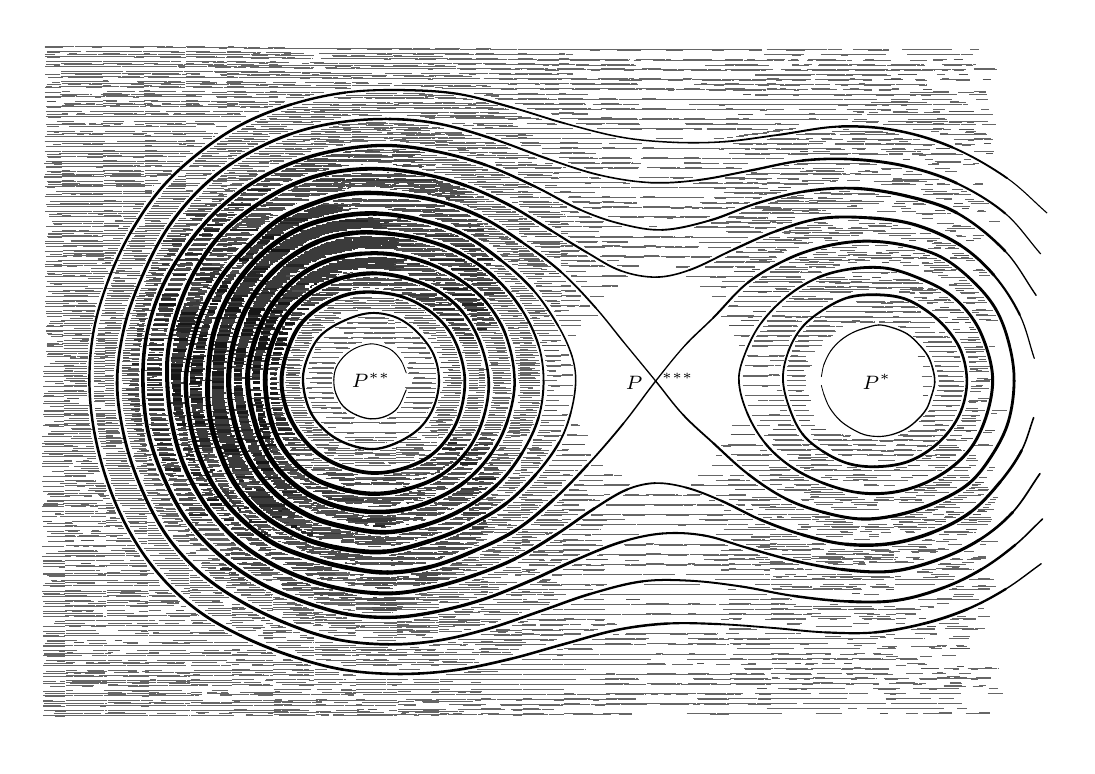
\begin{tikzpicture}[x=.08mm,y=-.08mm,line cap=round,line join=round]
\path[use as bounding box] (0,0) rectangle (1650,1140);

% Horizontal lithographic shading, separated from the contour lines.
% Each segment is editable in the same source-coordinate system.
\draw[black!60,line width=0.072mm,line cap=butt]
  (53,29) -- (62,29)
  (119,29) -- (140,29)
  (27,30) -- (74,30)
  (75,30) -- (122,30)
  (123,30) -- (170,30)
  (171,30) -- (218,30)
  (219,30) -- (230,30)
  (251,30) -- (282,30)
  (318,30) -- (328,30)
  (27,31) -- (56,31)
  (102,31) -- (118,31)
  (162,31) -- (184,31)
  (205,31) -- (252,31)
  (253,31) -- (300,31)
  (301,31) -- (348,31)
  (349,31) -- (369,31)
  (382,31) -- (408,31)
  (303,32) -- (316,32)
  (343,32) -- (390,32)
  (391,32) -- (438,32)
  (439,32) -- (486,32)
  (487,32) -- (492,32)
  (514,32) -- (531,32)
  (420,33) -- (447,33)
  (467,33) -- (514,33)
  (515,33) -- (562,33)
  (563,33) -- (610,33)
  (611,33) -- (638,33)
  (646,33) -- (687,33)
  (712,33) -- (735,33)
  (491,34) -- (513,34)
  (539,34) -- (579,34)
  (590,34) -- (637,34)
  (638,34) -- (685,34)
  (686,34) -- (733,34)
  (734,34) -- (772,34)
  (778,34) -- (825,34)
  (826,34) -- (834,34)
  (843,34) -- (881,34)
  (887,34) -- (896,34)
  (909,34) -- (956,34)
  (975,34) -- (1012,34)
  (1041,34) -- (1067,34)
  (1107,34) -- (1123,34)
  (1173,34) -- (1191,34)
  (1201,34) -- (1211,34)
  (1239,34) -- (1263,34)
  (1270,34) -- (1281,34)
  (1310,34) -- (1331,34)
  (1389,34) -- (1400,34)
  (1436,34) -- (1467,34)
  (1496,34) -- (1510,34)
  (630,35) -- (644,35)
  (695,35) -- (711,35)
  (736,35) -- (777,35)
  (793,35) -- (840,35)
  (841,35) -- (847,35)
  (853,35) -- (900,35)
  (901,35) -- (948,35)
  (949,35) -- (996,35)
  (997,35) -- (1044,35)
  (1045,35) -- (1092,35)
  (1093,35) -- (1140,35)
  (1141,35) -- (1166,35)
  (1174,35) -- (1221,35)
  (1222,35) -- (1269,35)
  (1270,35) -- (1293,35)
  (1310,35) -- (1357,35)
  (1358,35) -- (1368,35)
  (1388,35) -- (1435,35)
  (1436,35) -- (1468,35)
  (892,36) -- (908,36)
  (936,36) -- (973,36)
  (1013,36) -- (1040,36)
  (1086,36) -- (1106,36);
\draw[black!60,line width=0.072mm,line cap=butt]
  (1145,36) -- (1166,36)
  (1204,36) -- (1234,36)
  (1334,36) -- (1368,36)
  (53,37) -- (79,37)
  (119,37) -- (152,37)
  (185,37) -- (200,37)
  (31,38) -- (78,38)
  (79,38) -- (84,38)
  (92,38) -- (119,38)
  (135,38) -- (182,38)
  (183,38) -- (230,38)
  (231,38) -- (240,38)
  (251,38) -- (289,38)
  (317,38) -- (338,38)
  (31,39) -- (52,39)
  (227,39) -- (250,39)
  (268,39) -- (315,39)
  (316,39) -- (363,39)
  (364,39) -- (370,39)
  (379,39) -- (418,39)
  (358,40) -- (369,40)
  (407,40) -- (439,40)
  (463,40) -- (503,40)
  (514,40) -- (546,40)
  (580,40) -- (595,40)
  (65,41) -- (79,41)
  (119,41) -- (146,41)
  (185,41) -- (194,41)
  (478,41) -- (513,41)
  (522,41) -- (569,41)
  (570,41) -- (617,41)
  (618,41) -- (665,41)
  (666,41) -- (701,41)
  (712,41) -- (741,41)
  (778,41) -- (792,41)
  (844,41) -- (853,41)
  (27,42) -- (44,42)
  (63,42) -- (110,42)
  (111,42) -- (158,42)
  (159,42) -- (206,42)
  (207,42) -- (239,42)
  (251,42) -- (296,42)
  (317,42) -- (343,42)
  (554,42) -- (579,42)
  (612,42) -- (645,42)
  (662,42) -- (709,42)
  (710,42) -- (757,42)
  (758,42) -- (805,42)
  (806,42) -- (853,42)
  (854,42) -- (866,42)
  (1173,42) -- (1187,42)
  (1195,42) -- (1216,42)
  (1259,42) -- (1283,42)
  (1302,42) -- (1349,42)
  (1399,42) -- (1415,42)
  (1433,42) -- (1480,42)
  (1481,42) -- (1498,42)
  (214,43) -- (250,43)
  (258,43) -- (305,43)
  (306,43) -- (353,43)
  (354,43) -- (401,43)
  (402,43) -- (418,43)
  (744,43) -- (777,43)
  (810,43) -- (843,43)
  (1169,43) -- (1216,43)
  (1217,43) -- (1233,43)
  (1260,43) -- (1307,43)
  (1308,43) -- (1310,43)
  (1316,43) -- (1363,43)
  (1396,43) -- (1436,43)
  (1442,43) -- (1477,43)
  (1483,43) -- (1500,43)
  (356,44) -- (381,44)
  (393,44) -- (440,44)
  (441,44) -- (455,44);
\draw[black!60,line width=0.072mm,line cap=butt]
  (483,44) -- (507,44)
  (514,44) -- (536,44)
  (580,44) -- (594,44)
  (1213,44) -- (1227,44)
  (1291,44) -- (1302,44)
  (53,45) -- (100,45)
  (101,45) -- (106,45)
  (119,45) -- (155,45)
  (186,45) -- (214,45)
  (485,45) -- (532,45)
  (533,45) -- (580,45)
  (581,45) -- (628,45)
  (629,45) -- (660,45)
  (28,46) -- (75,46)
  (76,46) -- (123,46)
  (124,46) -- (171,46)
  (172,46) -- (219,46)
  (220,46) -- (244,46)
  (251,46) -- (298,46)
  (299,46) -- (301,46)
  (317,46) -- (342,46)
  (554,46) -- (579,46)
  (619,46) -- (645,46)
  (31,47) -- (52,47)
  (168,47) -- (184,47)
  (210,47) -- (251,47)
  (267,47) -- (314,47)
  (315,47) -- (362,47)
  (363,47) -- (410,47)
  (411,47) -- (424,47)
  (354,48) -- (383,48)
  (403,48) -- (450,48)
  (451,48) -- (452,48)
  (465,48) -- (503,48)
  (514,48) -- (548,48)
  (479,49) -- (515,49)
  (525,49) -- (572,49)
  (573,49) -- (620,49)
  (621,49) -- (668,49)
  (669,49) -- (705,49)
  (712,49) -- (746,49)
  (778,49) -- (802,49)
  (844,49) -- (860,49)
  (565,50) -- (577,50)
  (615,50) -- (648,50)
  (666,50) -- (713,50)
  (714,50) -- (761,50)
  (762,50) -- (809,50)
  (810,50) -- (857,50)
  (858,50) -- (905,50)
  (906,50) -- (953,50)
  (954,50) -- (956,50)
  (965,50) -- (1012,50)
  (1013,50) -- (1022,50)
  (1040,50) -- (1087,50)
  (1107,50) -- (1135,50)
  (1142,50) -- (1155,50)
  (1173,50) -- (1202,50)
  (1212,50) -- (1223,50)
  (1239,50) -- (1283,50)
  (1329,50) -- (1344,50)
  (1437,50) -- (1460,50)
  (809,51) -- (843,51)
  (861,51) -- (908,51)
  (916,51) -- (955,51)
  (962,51) -- (974,51)
  (993,51) -- (1040,51)
  (1041,51) -- (1088,51)
  (1089,51) -- (1136,51)
  (1137,51) -- (1184,51)
  (1185,51) -- (1201,51)
  (1207,51) -- (1225,51)
  (1237,51) -- (1246,51)
  (1252,51) -- (1299,51)
  (1300,51) -- (1308,51);
\draw[black!60,line width=0.072mm,line cap=butt]
  (1326,51) -- (1369,51)
  (1401,51) -- (1427,51)
  (1438,51) -- (1453,51)
  (1031,52) -- (1045,52)
  (1081,52) -- (1090,52)
  (1096,52) -- (1106,52)
  (1360,52) -- (1370,52)
  (53,53) -- (100,53)
  (101,53) -- (107,53)
  (119,53) -- (151,53)
  (185,53) -- (208,53)
  (29,54) -- (76,54)
  (77,54) -- (118,54)
  (131,54) -- (178,54)
  (179,54) -- (226,54)
  (227,54) -- (243,54)
  (252,54) -- (299,54)
  (300,54) -- (311,54)
  (317,54) -- (346,54)
  (384,54) -- (395,54)
  (277,55) -- (288,55)
  (294,55) -- (317,55)
  (330,55) -- (377,55)
  (378,55) -- (415,55)
  (448,55) -- (470,55)
  (367,56) -- (382,56)
  (436,56) -- (447,56)
  (454,56) -- (493,56)
  (499,56) -- (542,56)
  (580,56) -- (605,56)
  (53,57) -- (100,57)
  (101,57) -- (102,57)
  (119,57) -- (166,57)
  (185,57) -- (207,57)
  (251,57) -- (264,57)
  (494,57) -- (513,57)
  (531,57) -- (578,57)
  (579,57) -- (626,57)
  (627,57) -- (674,57)
  (675,57) -- (722,57)
  (723,57) -- (759,57)
  (778,57) -- (806,57)
  (844,57) -- (860,57)
  (29,58) -- (52,58)
  (58,58) -- (105,58)
  (106,58) -- (121,58)
  (142,58) -- (184,58)
  (200,58) -- (247,58)
  (248,58) -- (295,58)
  (296,58) -- (311,58)
  (317,58) -- (360,58)
  (383,58) -- (398,58)
  (635,58) -- (645,58)
  (683,58) -- (711,58)
  (726,58) -- (773,58)
  (774,58) -- (821,58)
  (822,58) -- (869,58)
  (870,58) -- (891,58)
  (910,58) -- (957,58)
  (958,58) -- (963,58)
  (1107,58) -- (1154,58)
  (1155,58) -- (1159,58)
  (1213,58) -- (1225,58)
  (1233,58) -- (1245,58)
  (1256,58) -- (1303,58)
  (1304,58) -- (1345,58)
  (1370,58) -- (1417,58)
  (1418,58) -- (1423,58)
  (1452,58) -- (1499,58)
  (1500,58) -- (1505,58)
  (41,59) -- (51,59)
  (239,59) -- (250,59)
  (286,59) -- (316,59)
  (339,59) -- (386,59)
  (387,59) -- (433,59);
\draw[black!60,line width=0.072mm,line cap=butt]
  (439,59) -- (477,59)
  (818,59) -- (827,59)
  (833,59) -- (843,59)
  (871,59) -- (918,59)
  (919,59) -- (966,59)
  (1075,59) -- (1122,59)
  (1123,59) -- (1170,59)
  (1171,59) -- (1177,59)
  (1213,59) -- (1241,59)
  (1255,59) -- (1302,59)
  (1303,59) -- (1309,59)
  (1316,59) -- (1363,59)
  (1364,59) -- (1411,59)
  (1412,59) -- (1424,59)
  (1455,59) -- (1483,59)
  (1490,59) -- (1501,59)
  (422,60) -- (469,60)
  (470,60) -- (517,60)
  (518,60) -- (565,60)
  (580,60) -- (620,60)
  (646,60) -- (663,60)
  (1087,60) -- (1106,60)
  (1148,60) -- (1158,60)
  (29,61) -- (42,61)
  (53,61) -- (100,61)
  (101,61) -- (148,61)
  (149,61) -- (196,61)
  (197,61) -- (221,61)
  (251,61) -- (270,61)
  (488,61) -- (513,61)
  (545,61) -- (592,61)
  (593,61) -- (640,61)
  (641,61) -- (680,61)
  (28,62) -- (75,62)
  (76,62) -- (118,62)
  (154,62) -- (184,62)
  (190,62) -- (237,62)
  (238,62) -- (285,62)
  (286,62) -- (333,62)
  (334,62) -- (367,62)
  (383,62) -- (404,62)
  (623,62) -- (644,62)
  (241,63) -- (250,63)
  (298,63) -- (322,63)
  (328,63) -- (347,63)
  (353,63) -- (400,63)
  (401,63) -- (448,63)
  (449,63) -- (455,63)
  (472,63) -- (491,63)
  (514,63) -- (528,63)
  (423,64) -- (453,64)
  (473,64) -- (520,64)
  (521,64) -- (568,64)
  (569,64) -- (616,64)
  (617,64) -- (626,64)
  (646,64) -- (676,64)
  (712,64) -- (733,64)
  (498,65) -- (512,65)
  (528,65) -- (575,65)
  (576,65) -- (579,65)
  (585,65) -- (632,65)
  (633,65) -- (680,65)
  (681,65) -- (728,65)
  (729,65) -- (767,65)
  (773,65) -- (820,65)
  (821,65) -- (826,65)
  (841,65) -- (883,65)
  (910,65) -- (948,65)
  (975,65) -- (1005,65)
  (1502,65) -- (1536,65)
  (635,66) -- (644,66)
  (686,66) -- (711,66)
  (735,66) -- (782,66)
  (783,66) -- (785,66)
  (792,66) -- (839,66);
\draw[black!60,line width=0.072mm,line cap=butt]
  (840,66) -- (887,66)
  (888,66) -- (935,66)
  (936,66) -- (983,66)
  (984,66) -- (1031,66)
  (1032,66) -- (1079,66)
  (1080,66) -- (1100,66)
  (1107,66) -- (1154,66)
  (1155,66) -- (1184,66)
  (1196,66) -- (1228,66)
  (1237,66) -- (1284,66)
  (1285,66) -- (1332,66)
  (1333,66) -- (1365,66)
  (1371,66) -- (1418,66)
  (1419,66) -- (1466,66)
  (1467,66) -- (1490,66)
  (1503,66) -- (1539,66)
  (821,67) -- (843,67)
  (894,67) -- (909,67)
  (946,67) -- (963,67)
  (1009,67) -- (1042,67)
  (1053,67) -- (1100,67)
  (1101,67) -- (1110,67)
  (1116,67) -- (1163,67)
  (1164,67) -- (1172,67)
  (1203,67) -- (1238,67)
  (1245,67) -- (1292,67)
  (1293,67) -- (1304,67)
  (1314,67) -- (1361,67)
  (1362,67) -- (1385,67)
  (1391,67) -- (1438,67)
  (1439,67) -- (1441,67)
  (1451,67) -- (1461,67)
  (1470,67) -- (1486,67)
  (53,69) -- (100,69)
  (101,69) -- (111,69)
  (117,69) -- (151,69)
  (157,69) -- (171,69)
  (185,69) -- (214,69)
  (251,69) -- (272,69)
  (317,69) -- (328,69)
  (73,70) -- (118,70)
  (156,70) -- (184,70)
  (200,70) -- (247,70)
  (248,70) -- (295,70)
  (296,70) -- (343,70)
  (344,70) -- (366,70)
  (383,70) -- (409,70)
  (297,71) -- (316,71)
  (339,71) -- (386,71)
  (387,71) -- (434,71)
  (435,71) -- (482,71)
  (120,72) -- (130,72)
  (436,72) -- (448,72)
  (464,72) -- (511,72)
  (512,72) -- (547,72)
  (575,72) -- (610,72)
  (646,72) -- (671,72)
  (712,72) -- (730,72)
  (53,73) -- (100,73)
  (101,73) -- (148,73)
  (149,73) -- (196,73)
  (197,73) -- (240,73)
  (251,73) -- (273,73)
  (317,73) -- (335,73)
  (567,73) -- (579,73)
  (624,73) -- (671,73)
  (684,73) -- (731,73)
  (732,73) -- (768,73)
  (774,73) -- (821,73)
  (822,73) -- (832,73)
  (840,73) -- (865,73)
  (28,74) -- (52,74)
  (75,74) -- (118,74)
  (160,74) -- (184,74)
  (197,74) -- (244,74);
\draw[black!60,line width=0.072mm,line cap=butt]
  (245,74) -- (253,74)
  (259,74) -- (273,74)
  (306,74) -- (353,74)
  (354,74) -- (401,74)
  (402,74) -- (416,74)
  (452,74) -- (462,74)
  (701,74) -- (711,74)
  (748,74) -- (795,74)
  (796,74) -- (843,74)
  (856,74) -- (865,74)
  (1155,74) -- (1202,74)
  (1203,74) -- (1250,74)
  (1251,74) -- (1298,74)
  (1299,74) -- (1346,74)
  (1347,74) -- (1364,74)
  (1443,74) -- (1456,74)
  (307,75) -- (316,75)
  (348,75) -- (385,75)
  (394,75) -- (441,75)
  (442,75) -- (489,75)
  (490,75) -- (493,75)
  (514,75) -- (536,75)
  (1155,75) -- (1202,75)
  (1203,75) -- (1243,75)
  (1269,75) -- (1310,75)
  (1325,75) -- (1370,75)
  (439,76) -- (448,76)
  (480,76) -- (527,76)
  (528,76) -- (570,76)
  (580,76) -- (627,76)
  (628,76) -- (629,76)
  (637,76) -- (684,76)
  (685,76) -- (691,76)
  (53,77) -- (100,77)
  (101,77) -- (148,77)
  (149,77) -- (178,77)
  (185,77) -- (224,77)
  (251,77) -- (282,77)
  (317,77) -- (327,77)
  (501,77) -- (513,77)
  (546,77) -- (569,77)
  (598,77) -- (645,77)
  (646,77) -- (648,77)
  (661,77) -- (706,77)
  (32,78) -- (56,78)
  (64,78) -- (111,78)
  (112,78) -- (119,78)
  (143,78) -- (184,78)
  (191,78) -- (238,78)
  (239,78) -- (286,78)
  (287,78) -- (334,78)
  (335,78) -- (370,78)
  (383,78) -- (417,78)
  (289,79) -- (316,79)
  (340,79) -- (387,79)
  (388,79) -- (435,79)
  (436,79) -- (483,79)
  (484,79) -- (493,79)
  (514,79) -- (533,79)
  (432,80) -- (448,80)
  (468,80) -- (515,80)
  (516,80) -- (563,80)
  (564,80) -- (611,80)
  (612,80) -- (633,80)
  (646,80) -- (690,80)
  (724,80) -- (745,80)
  (494,81) -- (514,81)
  (547,81) -- (579,81)
  (594,81) -- (641,81)
  (642,81) -- (689,81)
  (690,81) -- (718,81)
  (724,81) -- (771,81)
  (772,81) -- (819,81)
  (820,81) -- (867,81)
  (868,81) -- (888,81);
\draw[black!60,line width=0.072mm,line cap=butt]
  (906,81) -- (953,81)
  (954,81) -- (963,81)
  (971,81) -- (1006,81)
  (1041,81) -- (1054,81)
  (1173,81) -- (1193,81)
  (1305,81) -- (1314,81)
  (1371,81) -- (1386,81)
  (1452,81) -- (1463,81)
  (635,82) -- (644,82)
  (748,82) -- (777,82)
  (794,82) -- (841,82)
  (842,82) -- (848,82)
  (862,82) -- (909,82)
  (910,82) -- (957,82)
  (958,82) -- (1005,82)
  (1006,82) -- (1053,82)
  (1054,82) -- (1101,82)
  (1102,82) -- (1149,82)
  (1150,82) -- (1197,82)
  (1198,82) -- (1244,82)
  (1250,82) -- (1297,82)
  (1298,82) -- (1341,82)
  (1409,82) -- (1424,82)
  (1449,82) -- (1496,82)
  (938,83) -- (975,83)
  (1016,83) -- (1040,83)
  (1070,83) -- (1117,83)
  (1118,83) -- (1121,83)
  (1129,83) -- (1172,83)
  (1188,83) -- (1197,83)
  (1214,83) -- (1235,83)
  (1271,83) -- (1304,83)
  (1326,83) -- (1340,83)
  (1410,83) -- (1427,83)
  (1473,83) -- (1496,83)
  (119,84) -- (128,84)
  (53,85) -- (100,85)
  (101,85) -- (129,85)
  (174,85) -- (221,85)
  (222,85) -- (243,85)
  (251,85) -- (289,85)
  (317,85) -- (342,85)
  (39,86) -- (52,86)
  (175,86) -- (184,86)
  (217,86) -- (250,86)
  (276,86) -- (300,86)
  (315,86) -- (362,86)
  (363,86) -- (378,86)
  (390,86) -- (423,86)
  (449,86) -- (472,86)
  (407,87) -- (426,87)
  (440,87) -- (487,87)
  (488,87) -- (506,87)
  (515,87) -- (540,87)
  (487,88) -- (514,88)
  (521,88) -- (542,88)
  (556,88) -- (578,88)
  (594,88) -- (636,88)
  (642,88) -- (689,88)
  (690,88) -- (694,88)
  (712,88) -- (749,88)
  (778,88) -- (789,88)
  (54,89) -- (101,89)
  (102,89) -- (149,89)
  (150,89) -- (197,89)
  (198,89) -- (228,89)
  (251,89) -- (298,89)
  (299,89) -- (300,89)
  (317,89) -- (338,89)
  (566,89) -- (577,89)
  (628,89) -- (645,89)
  (677,89) -- (711,89)
  (717,89) -- (764,89)
  (765,89) -- (812,89)
  (813,89) -- (860,89);
\draw[black!60,line width=0.072mm,line cap=butt]
  (861,89) -- (901,89)
  (910,89) -- (957,89)
  (958,89) -- (968,89)
  (1069,89) -- (1078,89)
  (1107,89) -- (1129,89)
  (1173,89) -- (1188,89)
  (1319,89) -- (1329,89)
  (30,90) -- (53,90)
  (64,90) -- (85,90)
  (97,90) -- (118,90)
  (164,90) -- (184,90)
  (211,90) -- (250,90)
  (273,90) -- (320,90)
  (321,90) -- (368,90)
  (369,90) -- (416,90)
  (417,90) -- (424,90)
  (762,90) -- (777,90)
  (805,90) -- (814,90)
  (821,90) -- (843,90)
  (864,90) -- (911,90)
  (912,90) -- (959,90)
  (960,90) -- (969,90)
  (1058,90) -- (1105,90)
  (1106,90) -- (1153,90)
  (1154,90) -- (1201,90)
  (1202,90) -- (1249,90)
  (1250,90) -- (1274,90)
  (1282,90) -- (1329,90)
  (1330,90) -- (1377,90)
  (1378,90) -- (1425,90)
  (1426,90) -- (1427,90)
  (362,91) -- (382,91)
  (406,91) -- (450,91)
  (457,91) -- (491,91)
  (515,91) -- (539,91)
  (1089,91) -- (1106,91)
  (1159,91) -- (1177,91)
  (1195,91) -- (1226,91)
  (1291,91) -- (1303,91)
  (1327,91) -- (1370,91)
  (1415,91) -- (1427,91)
  (119,92) -- (132,92)
  (185,92) -- (197,92)
  (474,92) -- (514,92)
  (520,92) -- (567,92)
  (568,92) -- (575,92)
  (581,92) -- (628,92)
  (629,92) -- (676,92)
  (677,92) -- (703,92)
  (712,92) -- (729,92)
  (29,93) -- (38,93)
  (50,93) -- (97,93)
  (98,93) -- (145,93)
  (146,93) -- (193,93)
  (194,93) -- (241,93)
  (242,93) -- (243,93)
  (251,93) -- (292,93)
  (317,93) -- (344,93)
  (383,93) -- (398,93)
  (625,93) -- (645,93)
  (667,93) -- (711,93)
  (721,93) -- (735,93)
  (28,94) -- (53,94)
  (93,94) -- (118,94)
  (158,94) -- (184,94)
  (208,94) -- (250,94)
  (263,94) -- (310,94)
  (311,94) -- (358,94)
  (359,94) -- (406,94)
  (407,94) -- (442,94)
  (449,94) -- (476,94)
  (357,95) -- (382,95)
  (405,95) -- (452,95)
  (453,95) -- (500,95)
  (501,95) -- (507,95);
\draw[black!60,line width=0.072mm,line cap=butt]
  (646,95) -- (660,95)
  (488,96) -- (513,96)
  (657,96) -- (704,96)
  (705,96) -- (752,96)
  (753,96) -- (757,96)
  (778,96) -- (794,96)
  (844,96) -- (860,96)
  (672,97) -- (711,97)
  (725,97) -- (772,97)
  (773,97) -- (820,97)
  (821,97) -- (868,97)
  (869,97) -- (916,97)
  (917,97) -- (964,97)
  (965,97) -- (1012,97)
  (1013,97) -- (1026,97)
  (1042,97) -- (1068,97)
  (1107,97) -- (1138,97)
  (1173,97) -- (1189,97)
  (1195,97) -- (1204,97)
  (1244,97) -- (1274,97)
  (1305,97) -- (1320,97)
  (1372,97) -- (1383,97)
  (751,98) -- (777,98)
  (813,98) -- (843,98)
  (864,98) -- (909,98)
  (922,98) -- (969,98)
  (970,98) -- (975,98)
  (981,98) -- (1028,98)
  (1029,98) -- (1076,98)
  (1077,98) -- (1124,98)
  (1125,98) -- (1172,98)
  (1173,98) -- (1220,98)
  (1221,98) -- (1238,98)
  (1245,98) -- (1285,98)
  (1294,98) -- (1341,98)
  (1351,98) -- (1383,98)
  (1016,99) -- (1026,99)
  (1081,99) -- (1108,99)
  (1119,99) -- (1166,99)
  (1167,99) -- (1172,99)
  (1216,99) -- (1225,99)
  (1327,99) -- (1340,99)
  (1351,99) -- (1370,99)
  (185,100) -- (194,100)
  (54,101) -- (67,101)
  (126,101) -- (171,101)
  (177,101) -- (224,101)
  (225,101) -- (236,101)
  (245,101) -- (281,101)
  (317,101) -- (346,101)
  (384,101) -- (396,101)
  (1437,101) -- (1462,101)
  (1503,101) -- (1522,101)
  (27,102) -- (53,102)
  (293,102) -- (317,102)
  (328,102) -- (375,102)
  (376,102) -- (423,102)
  (424,102) -- (436,102)
  (449,102) -- (469,102)
  (1401,102) -- (1448,102)
  (1449,102) -- (1462,102)
  (1477,102) -- (1502,102)
  (1510,102) -- (1522,102)
  (415,103) -- (448,103)
  (460,103) -- (470,103)
  (1403,103) -- (1414,103)
  (1420,103) -- (1436,103)
  (1488,103) -- (1502,103)
  (120,104) -- (149,104)
  (185,104) -- (202,104)
  (537,104) -- (584,104)
  (585,104) -- (587,104)
  (596,104) -- (630,104)
  (708,104) -- (739,104)
  (778,104) -- (810,104);
\draw[black!60,line width=0.072mm,line cap=butt]
  (844,104) -- (855,104)
  (51,105) -- (98,105)
  (99,105) -- (102,105)
  (116,105) -- (163,105)
  (164,105) -- (211,105)
  (212,105) -- (259,105)
  (260,105) -- (307,105)
  (317,105) -- (347,105)
  (383,105) -- (402,105)
  (621,105) -- (644,105)
  (727,105) -- (774,105)
  (775,105) -- (822,105)
  (823,105) -- (870,105)
  (871,105) -- (890,105)
  (1173,105) -- (1203,105)
  (1239,105) -- (1283,105)
  (1305,105) -- (1331,105)
  (1371,105) -- (1386,105)
  (1437,105) -- (1464,105)
  (1495,105) -- (1523,105)
  (216,106) -- (250,106)
  (286,106) -- (316,106)
  (333,106) -- (348,106)
  (363,106) -- (410,106)
  (411,106) -- (435,106)
  (441,106) -- (455,106)
  (763,106) -- (777,106)
  (811,106) -- (821,106)
  (828,106) -- (843,106)
  (866,106) -- (888,106)
  (1155,106) -- (1202,106)
  (1203,106) -- (1250,106)
  (1251,106) -- (1298,106)
  (1299,106) -- (1346,106)
  (1347,106) -- (1394,106)
  (1395,106) -- (1442,106)
  (1443,106) -- (1475,106)
  (1495,106) -- (1518,106)
  (416,107) -- (448,107)
  (506,107) -- (553,107)
  (554,107) -- (564,107)
  (581,107) -- (620,107)
  (646,107) -- (669,107)
  (1155,107) -- (1175,107)
  (1215,107) -- (1225,107)
  (1280,107) -- (1308,107)
  (1346,107) -- (1375,107)
  (1401,107) -- (1410,107)
  (1418,107) -- (1434,107)
  (54,108) -- (78,108)
  (120,108) -- (159,108)
  (185,108) -- (214,108)
  (251,108) -- (268,108)
  (526,108) -- (573,108)
  (574,108) -- (580,108)
  (587,108) -- (634,108)
  (635,108) -- (677,108)
  (725,108) -- (749,108)
  (28,109) -- (75,109)
  (76,109) -- (123,109)
  (124,109) -- (171,109)
  (172,109) -- (219,109)
  (220,109) -- (267,109)
  (268,109) -- (276,109)
  (299,109) -- (346,109)
  (347,109) -- (356,109)
  (383,109) -- (397,109)
  (630,109) -- (645,109)
  (735,109) -- (748,109)
  (28,110) -- (53,110)
  (107,110) -- (117,110)
  (167,110) -- (176,110)
  (300,110) -- (317,110)
  (328,110) -- (375,110)
  (376,110) -- (398,110);
\draw[black!60,line width=0.072mm,line cap=butt]
  (410,110) -- (438,110)
  (373,111) -- (382,111)
  (486,111) -- (533,111)
  (534,111) -- (581,111)
  (582,111) -- (629,111)
  (630,111) -- (636,111)
  (646,111) -- (680,111)
  (493,112) -- (514,112)
  (537,112) -- (546,112)
  (552,112) -- (599,112)
  (600,112) -- (645,112)
  (651,112) -- (698,112)
  (742,112) -- (771,112)
  (778,112) -- (825,112)
  (826,112) -- (827,112)
  (842,112) -- (882,112)
  (907,112) -- (934,112)
  (976,112) -- (998,112)
  (691,113) -- (707,113)
  (746,113) -- (793,113)
  (794,113) -- (841,113)
  (842,113) -- (889,113)
  (890,113) -- (937,113)
  (938,113) -- (985,113)
  (986,113) -- (1033,113)
  (1034,113) -- (1081,113)
  (1082,113) -- (1129,113)
  (1130,113) -- (1146,113)
  (1173,113) -- (1206,113)
  (1239,113) -- (1286,113)
  (1287,113) -- (1291,113)
  (1305,113) -- (1333,113)
  (1371,113) -- (1396,113)
  (1437,113) -- (1467,113)
  (1506,113) -- (1525,113)
  (880,114) -- (910,114)
  (947,114) -- (994,114)
  (995,114) -- (1041,114)
  (1056,114) -- (1103,114)
  (1104,114) -- (1151,114)
  (1152,114) -- (1199,114)
  (1200,114) -- (1247,114)
  (1248,114) -- (1295,114)
  (1296,114) -- (1343,114)
  (1344,114) -- (1349,114)
  (1379,114) -- (1400,114)
  (1420,114) -- (1467,114)
  (120,116) -- (142,116)
  (185,116) -- (207,116)
  (251,116) -- (271,116)
  (75,117) -- (119,117)
  (125,117) -- (142,117)
  (161,117) -- (187,117)
  (195,117) -- (242,117)
  (243,117) -- (290,117)
  (291,117) -- (338,117)
  (339,117) -- (361,117)
  (383,117) -- (408,117)
  (1371,117) -- (1398,117)
  (1464,117) -- (1479,117)
  (300,118) -- (316,118)
  (336,118) -- (382,118)
  (393,118) -- (407,118)
  (453,118) -- (491,118)
  (515,118) -- (530,118)
  (1339,118) -- (1386,118)
  (1387,118) -- (1427,118)
  (1464,118) -- (1490,118)
  (474,119) -- (521,119)
  (522,119) -- (569,119)
  (570,119) -- (575,119)
  (581,119) -- (627,119)
  (647,119) -- (679,119)
  (712,119) -- (727,119)
  (1409,119) -- (1424,119);
\draw[black!60,line width=0.072mm,line cap=butt]
  (57,120) -- (85,120)
  (93,120) -- (107,120)
  (120,120) -- (167,120)
  (168,120) -- (171,120)
  (185,120) -- (198,120)
  (213,120) -- (227,120)
  (251,120) -- (272,120)
  (317,120) -- (334,120)
  (554,120) -- (580,120)
  (588,120) -- (605,120)
  (611,120) -- (658,120)
  (659,120) -- (706,120)
  (707,120) -- (732,120)
  (773,120) -- (820,120)
  (821,120) -- (835,120)
  (844,120) -- (885,120)
  (910,120) -- (939,120)
  (60,121) -- (107,121)
  (108,121) -- (119,121)
  (141,121) -- (188,121)
  (189,121) -- (199,121)
  (214,121) -- (261,121)
  (262,121) -- (274,121)
  (287,121) -- (334,121)
  (335,121) -- (382,121)
  (383,121) -- (402,121)
  (449,121) -- (464,121)
  (699,121) -- (711,121)
  (787,121) -- (834,121)
  (835,121) -- (882,121)
  (883,121) -- (887,121)
  (897,121) -- (944,121)
  (945,121) -- (971,121)
  (1050,121) -- (1097,121)
  (1098,121) -- (1102,121)
  (1108,121) -- (1155,121)
  (1156,121) -- (1157,121)
  (1173,121) -- (1207,121)
  (1239,121) -- (1284,121)
  (1305,121) -- (1317,121)
  (1326,121) -- (1341,121)
  (1371,121) -- (1416,121)
  (1437,121) -- (1484,121)
  (1485,121) -- (1491,121)
  (240,122) -- (250,122)
  (355,122) -- (382,122)
  (436,122) -- (483,122)
  (484,122) -- (494,122)
  (515,122) -- (537,122)
  (581,122) -- (590,122)
  (823,122) -- (843,122)
  (1053,122) -- (1100,122)
  (1101,122) -- (1148,122)
  (1149,122) -- (1196,122)
  (1197,122) -- (1244,122)
  (1245,122) -- (1292,122)
  (1293,122) -- (1340,122)
  (1341,122) -- (1388,122)
  (1389,122) -- (1436,122)
  (1437,122) -- (1484,122)
  (1485,122) -- (1493,122)
  (480,123) -- (527,123)
  (528,123) -- (575,123)
  (576,123) -- (623,123)
  (624,123) -- (641,123)
  (647,123) -- (690,123)
  (712,123) -- (743,123)
  (1098,123) -- (1107,123)
  (1287,123) -- (1303,123)
  (1329,123) -- (1348,123)
  (1356,123) -- (1367,123)
  (1387,123) -- (1396,123)
  (54,124) -- (73,124)
  (120,124) -- (147,124)
  (186,124) -- (211,124);
\draw[black!60,line width=0.072mm,line cap=butt]
  (251,124) -- (278,124)
  (317,124) -- (329,124)
  (557,124) -- (580,124)
  (610,124) -- (657,124)
  (658,124) -- (705,124)
  (706,124) -- (746,124)
  (29,125) -- (76,125)
  (77,125) -- (124,125)
  (130,125) -- (177,125)
  (178,125) -- (188,125)
  (194,125) -- (241,125)
  (242,125) -- (289,125)
  (290,125) -- (337,125)
  (338,125) -- (369,125)
  (375,125) -- (389,125)
  (30,126) -- (53,126)
  (302,126) -- (316,126)
  (337,126) -- (347,126)
  (353,126) -- (382,126)
  (421,126) -- (444,126)
  (451,126) -- (492,126)
  (515,126) -- (527,126)
  (433,127) -- (445,127)
  (481,127) -- (528,127)
  (529,127) -- (576,127)
  (577,127) -- (624,127)
  (625,127) -- (672,127)
  (673,127) -- (685,127)
  (694,127) -- (703,127)
  (712,127) -- (739,127)
  (554,128) -- (584,128)
  (613,128) -- (660,128)
  (661,128) -- (708,128)
  (709,128) -- (756,128)
  (757,128) -- (760,128)
  (793,128) -- (840,128)
  (841,128) -- (888,128)
  (889,128) -- (894,128)
  (910,128) -- (957,128)
  (958,128) -- (964,128)
  (976,128) -- (1013,128)
  (1108,128) -- (1119,128)
  (449,129) -- (461,129)
  (731,129) -- (764,129)
  (805,129) -- (843,129)
  (849,129) -- (896,129)
  (897,129) -- (911,129)
  (918,129) -- (965,129)
  (966,129) -- (1013,129)
  (1014,129) -- (1061,129)
  (1062,129) -- (1109,129)
  (1110,129) -- (1157,129)
  (1158,129) -- (1162,129)
  (1174,129) -- (1199,129)
  (1239,129) -- (1283,129)
  (1305,129) -- (1341,129)
  (1437,129) -- (1456,129)
  (1514,129) -- (1526,129)
  (412,130) -- (459,130)
  (460,130) -- (494,130)
  (515,130) -- (528,130)
  (890,130) -- (908,130)
  (935,130) -- (951,130)
  (957,130) -- (975,130)
  (1004,130) -- (1044,130)
  (1067,130) -- (1114,130)
  (1124,130) -- (1171,130)
  (1172,130) -- (1200,130)
  (1224,130) -- (1246,130)
  (1252,130) -- (1283,130)
  (1300,130) -- (1347,130)
  (1348,130) -- (1370,130)
  (1395,130) -- (1413,130)
  (1443,130) -- (1457,130)
  (438,131) -- (448,131);
\draw[black!60,line width=0.072mm,line cap=butt]
  (464,131) -- (511,131)
  (512,131) -- (559,131)
  (1162,131) -- (1173,131)
  (1355,131) -- (1370,131)
  (54,132) -- (86,132)
  (120,132) -- (167,132)
  (186,132) -- (210,132)
  (251,132) -- (288,132)
  (317,132) -- (339,132)
  (29,133) -- (76,133)
  (77,133) -- (87,133)
  (99,133) -- (119,133)
  (154,133) -- (185,133)
  (220,133) -- (252,133)
  (268,133) -- (289,133)
  (295,133) -- (342,133)
  (343,133) -- (367,133)
  (402,133) -- (426,133)
  (449,133) -- (472,133)
  (1310,133) -- (1328,133)
  (1373,133) -- (1397,133)
  (1437,133) -- (1449,133)
  (408,134) -- (448,134)
  (454,134) -- (501,134)
  (502,134) -- (549,134)
  (550,134) -- (551,134)
  (581,134) -- (598,134)
  (1316,134) -- (1328,134)
  (1335,134) -- (1350,134)
  (1373,134) -- (1413,134)
  (1423,134) -- (1449,134)
  (489,135) -- (514,135)
  (526,135) -- (573,135)
  (574,135) -- (621,135)
  (622,135) -- (669,135)
  (670,135) -- (717,135)
  (718,135) -- (749,135)
  (844,135) -- (868,135)
  (54,136) -- (64,136)
  (78,136) -- (91,136)
  (120,136) -- (167,136)
  (168,136) -- (174,136)
  (186,136) -- (223,136)
  (233,136) -- (244,136)
  (251,136) -- (281,136)
  (317,136) -- (337,136)
  (624,136) -- (651,136)
  (677,136) -- (712,136)
  (730,136) -- (777,136)
  (831,136) -- (878,136)
  (879,136) -- (889,136)
  (1241,136) -- (1250,136)
  (30,137) -- (64,137)
  (77,137) -- (119,137)
  (137,137) -- (184,137)
  (185,137) -- (188,137)
  (196,137) -- (225,137)
  (231,137) -- (278,137)
  (279,137) -- (326,137)
  (327,137) -- (338,137)
  (388,137) -- (434,137)
  (449,137) -- (470,137)
  (833,137) -- (843,137)
  (864,137) -- (890,137)
  (1170,137) -- (1217,137)
  (1218,137) -- (1265,137)
  (1266,137) -- (1313,137)
  (1314,137) -- (1325,137)
  (1333,137) -- (1354,137)
  (1371,137) -- (1418,137)
  (1419,137) -- (1424,137)
  (1432,137) -- (1479,137)
  (1480,137) -- (1527,137)
  (1528,137) -- (1533,137)
  (33,138) -- (53,138);
\draw[black!60,line width=0.072mm,line cap=butt]
  (403,138) -- (450,138)
  (451,138) -- (498,138)
  (499,138) -- (508,138)
  (515,138) -- (541,138)
  (1179,138) -- (1189,138)
  (1195,138) -- (1240,138)
  (1273,138) -- (1304,138)
  (1333,138) -- (1370,138)
  (1376,138) -- (1423,138)
  (1424,138) -- (1440,138)
  (1446,138) -- (1493,138)
  (1494,138) -- (1502,138)
  (485,139) -- (514,139)
  (526,139) -- (562,139)
  (602,139) -- (649,139)
  (650,139) -- (697,139)
  (698,139) -- (741,139)
  (54,140) -- (101,140)
  (102,140) -- (109,140)
  (115,140) -- (162,140)
  (163,140) -- (175,140)
  (186,140) -- (233,140)
  (234,140) -- (240,140)
  (252,140) -- (293,140)
  (317,140) -- (345,140)
  (383,140) -- (396,140)
  (623,140) -- (646,140)
  (670,140) -- (712,140)
  (718,140) -- (765,140)
  (766,140) -- (785,140)
  (29,141) -- (76,141)
  (77,141) -- (119,141)
  (125,141) -- (172,141)
  (173,141) -- (186,141)
  (192,141) -- (239,141)
  (240,141) -- (253,141)
  (259,141) -- (306,141)
  (307,141) -- (347,141)
  (380,141) -- (427,141)
  (428,141) -- (434,141)
  (449,141) -- (472,141)
  (32,142) -- (53,142)
  (415,142) -- (462,142)
  (463,142) -- (497,142)
  (713,142) -- (723,142)
  (630,143) -- (677,143)
  (678,143) -- (725,143)
  (726,143) -- (758,143)
  (778,143) -- (799,143)
  (910,143) -- (927,143)
  (383,144) -- (396,144)
  (637,144) -- (646,144)
  (680,144) -- (727,144)
  (728,144) -- (775,144)
  (776,144) -- (812,144)
  (845,144) -- (892,144)
  (893,144) -- (940,144)
  (941,144) -- (968,144)
  (976,144) -- (1023,144)
  (1024,144) -- (1034,144)
  (1042,144) -- (1076,144)
  (1108,144) -- (1129,144)
  (1135,144) -- (1145,144)
  (1241,144) -- (1251,144)
  (1444,144) -- (1456,144)
  (369,145) -- (378,145)
  (384,145) -- (431,145)
  (432,145) -- (435,145)
  (445,145) -- (472,145)
  (762,145) -- (777,145)
  (807,145) -- (816,145)
  (874,145) -- (921,145)
  (922,145) -- (969,145)
  (970,145) -- (1017,145)
  (1018,145) -- (1065,145);
\draw[black!60,line width=0.072mm,line cap=butt]
  (1066,145) -- (1113,145)
  (1114,145) -- (1161,145)
  (1162,145) -- (1209,145)
  (1210,145) -- (1257,145)
  (1258,145) -- (1302,145)
  (1312,145) -- (1332,145)
  (1397,145) -- (1427,145)
  (1433,145) -- (1460,145)
  (421,146) -- (463,146)
  (469,146) -- (486,146)
  (1021,146) -- (1040,146)
  (1091,146) -- (1111,146)
  (1121,146) -- (1168,146)
  (1169,146) -- (1173,146)
  (1188,146) -- (1235,146)
  (1236,146) -- (1250,146)
  (1279,146) -- (1303,146)
  (1400,146) -- (1436,146)
  (54,148) -- (74,148)
  (120,148) -- (153,148)
  (185,148) -- (232,148)
  (233,148) -- (240,148)
  (266,148) -- (295,148)
  (317,148) -- (339,148)
  (383,148) -- (395,148)
  (1443,148) -- (1455,148)
  (1503,148) -- (1524,148)
  (46,149) -- (74,149)
  (168,149) -- (185,149)
  (209,149) -- (251,149)
  (270,149) -- (316,149)
  (361,149) -- (408,149)
  (409,149) -- (435,149)
  (449,149) -- (465,149)
  (1309,149) -- (1351,149)
  (1366,149) -- (1413,149)
  (1414,149) -- (1461,149)
  (1462,149) -- (1509,149)
  (1510,149) -- (1525,149)
  (364,150) -- (382,150)
  (421,150) -- (453,150)
  (537,150) -- (569,150)
  (1331,150) -- (1350,150)
  (1394,150) -- (1406,150)
  (1412,150) -- (1436,150)
  (1462,150) -- (1484,150)
  (1491,150) -- (1502,150)
  (525,151) -- (572,151)
  (573,151) -- (600,151)
  (673,151) -- (694,151)
  (707,151) -- (754,151)
  (755,151) -- (762,151)
  (792,151) -- (806,151)
  (54,152) -- (91,152)
  (97,152) -- (109,152)
  (116,152) -- (152,152)
  (186,152) -- (233,152)
  (234,152) -- (245,152)
  (251,152) -- (296,152)
  (727,152) -- (770,152)
  (792,152) -- (837,152)
  (870,152) -- (917,152)
  (918,152) -- (965,152)
  (966,152) -- (970,152)
  (1043,152) -- (1088,152)
  (1108,152) -- (1127,152)
  (1186,152) -- (1196,152)
  (1438,152) -- (1454,152)
  (29,153) -- (76,153)
  (77,153) -- (92,153)
  (98,153) -- (119,153)
  (137,153) -- (148,153)
  (171,153) -- (185,153)
  (221,153) -- (251,153)
  (269,153) -- (297,153);
\draw[black!60,line width=0.072mm,line cap=butt]
  (354,153) -- (401,153)
  (402,153) -- (433,153)
  (439,153) -- (454,153)
  (824,153) -- (840,153)
  (887,153) -- (912,153)
  (937,153) -- (972,153)
  (1045,153) -- (1092,153)
  (1093,153) -- (1140,153)
  (1141,153) -- (1188,153)
  (1189,153) -- (1225,153)
  (1371,153) -- (1418,153)
  (1419,153) -- (1466,153)
  (1467,153) -- (1475,153)
  (1481,153) -- (1505,153)
  (1515,153) -- (1537,153)
  (424,154) -- (446,154)
  (492,154) -- (539,154)
  (540,154) -- (566,154)
  (581,154) -- (614,154)
  (713,154) -- (724,154)
  (1084,154) -- (1107,154)
  (1157,154) -- (1170,154)
  (1199,154) -- (1224,154)
  (1358,154) -- (1370,154)
  (1385,154) -- (1432,154)
  (1433,154) -- (1480,154)
  (1481,154) -- (1502,154)
  (120,155) -- (131,155)
  (188,155) -- (197,155)
  (499,155) -- (512,155)
  (537,155) -- (580,155)
  (588,155) -- (635,155)
  (636,155) -- (637,155)
  (691,155) -- (708,155)
  (714,155) -- (761,155)
  (762,155) -- (771,155)
  (66,156) -- (113,156)
  (114,156) -- (161,156)
  (162,156) -- (209,156)
  (210,156) -- (257,156)
  (258,156) -- (268,156)
  (299,156) -- (312,156)
  (383,156) -- (409,156)
  (748,156) -- (778,156)
  (30,157) -- (49,157)
  (69,157) -- (116,157)
  (117,157) -- (119,157)
  (160,157) -- (185,157)
  (222,157) -- (251,157)
  (299,157) -- (317,157)
  (370,157) -- (412,157)
  (485,157) -- (494,157)
  (479,158) -- (526,158)
  (527,158) -- (574,158)
  (575,158) -- (622,158)
  (623,158) -- (635,158)
  (642,158) -- (654,158)
  (726,158) -- (739,158)
  (500,159) -- (514,159)
  (550,159) -- (580,159)
  (603,159) -- (650,159)
  (651,159) -- (661,159)
  (705,159) -- (752,159)
  (753,159) -- (800,159)
  (801,159) -- (830,159)
  (836,159) -- (863,159)
  (910,159) -- (949,159)
  (976,159) -- (1014,159)
  (1042,159) -- (1052,159)
  (340,160) -- (363,160)
  (383,160) -- (407,160)
  (747,160) -- (778,160)
  (792,160) -- (839,160)
  (840,160) -- (866,160)
  (904,160) -- (951,160);
\draw[black!60,line width=0.072mm,line cap=butt]
  (952,160) -- (999,160)
  (1000,160) -- (1047,160)
  (1048,160) -- (1070,160)
  (1078,160) -- (1125,160)
  (1126,160) -- (1150,160)
  (1209,160) -- (1219,160)
  (1437,160) -- (1454,160)
  (339,161) -- (386,161)
  (387,161) -- (421,161)
  (465,161) -- (482,161)
  (956,161) -- (975,161)
  (998,161) -- (1041,161)
  (1058,161) -- (1070,161)
  (1078,161) -- (1125,161)
  (1126,161) -- (1173,161)
  (1174,161) -- (1175,161)
  (1191,161) -- (1215,161)
  (1405,161) -- (1452,161)
  (1453,161) -- (1466,161)
  (373,162) -- (382,162)
  (466,162) -- (513,162)
  (514,162) -- (561,162)
  (562,162) -- (569,162)
  (585,162) -- (624,162)
  (1084,162) -- (1107,162)
  (1187,162) -- (1207,162)
  (1294,162) -- (1304,162)
  (1414,162) -- (1436,162)
  (502,163) -- (514,163)
  (554,163) -- (577,163)
  (597,163) -- (639,163)
  (1184,163) -- (1199,163)
  (54,164) -- (75,164)
  (83,164) -- (103,164)
  (123,164) -- (170,164)
  (181,164) -- (228,164)
  (229,164) -- (245,164)
  (252,164) -- (283,164)
  (332,164) -- (350,164)
  (358,164) -- (370,164)
  (383,164) -- (407,164)
  (1177,164) -- (1195,164)
  (1308,164) -- (1326,164)
  (1337,164) -- (1351,164)
  (30,165) -- (58,165)
  (65,165) -- (74,165)
  (86,165) -- (104,165)
  (158,165) -- (170,165)
  (232,165) -- (251,165)
  (358,165) -- (405,165)
  (406,165) -- (413,165)
  (449,165) -- (490,165)
  (515,165) -- (529,165)
  (1174,165) -- (1184,165)
  (1277,165) -- (1324,165)
  (1325,165) -- (1358,165)
  (1434,165) -- (1446,165)
  (1489,165) -- (1505,165)
  (41,166) -- (50,166)
  (472,166) -- (519,166)
  (520,166) -- (563,166)
  (571,166) -- (618,166)
  (619,166) -- (624,166)
  (647,166) -- (690,166)
  (1168,166) -- (1177,166)
  (1329,166) -- (1366,166)
  (1488,166) -- (1502,166)
  (121,167) -- (132,167)
  (252,167) -- (265,167)
  (571,167) -- (580,167)
  (592,167) -- (639,167)
  (640,167) -- (656,167)
  (662,167) -- (690,167)
  (727,167) -- (774,167)
  (775,167) -- (822,167);
\draw[black!60,line width=0.072mm,line cap=butt]
  (823,167) -- (870,167)
  (871,167) -- (893,167)
  (1159,167) -- (1173,167)
  (54,168) -- (101,168)
  (102,168) -- (149,168)
  (150,168) -- (190,168)
  (200,168) -- (247,168)
  (248,168) -- (295,168)
  (296,168) -- (302,168)
  (325,168) -- (372,168)
  (383,168) -- (402,168)
  (449,168) -- (465,168)
  (758,168) -- (778,168)
  (794,168) -- (841,168)
  (842,168) -- (889,168)
  (890,168) -- (895,168)
  (1150,168) -- (1166,168)
  (1234,168) -- (1281,168)
  (1306,168) -- (1329,168)
  (1363,168) -- (1377,168)
  (1449,168) -- (1461,168)
  (1503,168) -- (1522,168)
  (30,169) -- (58,169)
  (79,169) -- (89,169)
  (98,169) -- (119,169)
  (167,169) -- (185,169)
  (230,169) -- (251,169)
  (358,169) -- (382,169)
  (433,169) -- (480,169)
  (481,169) -- (506,169)
  (515,169) -- (548,169)
  (581,169) -- (599,169)
  (1137,169) -- (1159,169)
  (1227,169) -- (1274,169)
  (1275,169) -- (1283,169)
  (1289,169) -- (1336,169)
  (1337,169) -- (1384,169)
  (1448,169) -- (1495,169)
  (1496,169) -- (1523,169)
  (431,170) -- (448,170)
  (478,170) -- (514,170)
  (520,170) -- (567,170)
  (568,170) -- (615,170)
  (616,170) -- (663,170)
  (664,170) -- (693,170)
  (779,170) -- (791,170)
  (1138,170) -- (1152,170)
  (1220,170) -- (1241,170)
  (1289,170) -- (1304,170)
  (1324,170) -- (1371,170)
  (1372,170) -- (1377,170)
  (1470,170) -- (1502,170)
  (186,171) -- (195,171)
  (601,171) -- (646,171)
  (667,171) -- (705,171)
  (742,171) -- (789,171)
  (790,171) -- (802,171)
  (1129,171) -- (1144,171)
  (54,172) -- (101,172)
  (102,172) -- (149,172)
  (150,172) -- (197,172)
  (198,172) -- (245,172)
  (246,172) -- (293,172)
  (294,172) -- (298,172)
  (319,172) -- (366,172)
  (367,172) -- (371,172)
  (449,172) -- (469,172)
  (759,172) -- (778,172)
  (1125,172) -- (1137,172)
  (27,173) -- (74,173)
  (75,173) -- (119,173)
  (146,173) -- (185,173)
  (227,173) -- (251,173)
  (339,173) -- (385,173)
  (421,173) -- (468,173);
\draw[black!60,line width=0.072mm,line cap=butt]
  (469,173) -- (496,173)
  (515,173) -- (540,173)
  (477,174) -- (524,174)
  (525,174) -- (572,174)
  (573,174) -- (620,174)
  (621,174) -- (668,174)
  (669,174) -- (695,174)
  (779,174) -- (792,174)
  (1110,174) -- (1119,174)
  (566,175) -- (580,175)
  (594,175) -- (641,175)
  (642,175) -- (646,175)
  (652,175) -- (699,175)
  (700,175) -- (720,175)
  (752,175) -- (799,175)
  (800,175) -- (847,175)
  (848,175) -- (895,175)
  (896,175) -- (926,175)
  (997,175) -- (1022,175)
  (278,176) -- (293,176)
  (313,176) -- (360,176)
  (449,176) -- (464,176)
  (698,176) -- (708,176)
  (764,176) -- (778,176)
  (788,176) -- (835,176)
  (836,176) -- (845,176)
  (852,176) -- (899,176)
  (900,176) -- (934,176)
  (1007,176) -- (1040,176)
  (1089,176) -- (1105,176)
  (1178,176) -- (1224,176)
  (1235,176) -- (1246,176)
  (1259,176) -- (1277,176)
  (1308,176) -- (1333,176)
  (1376,176) -- (1389,176)
  (1503,176) -- (1530,176)
  (344,177) -- (382,177)
  (411,177) -- (458,177)
  (459,177) -- (494,177)
  (515,177) -- (534,177)
  (581,177) -- (600,177)
  (1173,177) -- (1220,177)
  (1221,177) -- (1240,177)
  (1261,177) -- (1295,177)
  (1309,177) -- (1356,177)
  (1357,177) -- (1404,177)
  (1405,177) -- (1417,177)
  (1470,177) -- (1517,177)
  (1518,177) -- (1532,177)
  (437,178) -- (448,178)
  (474,178) -- (521,178)
  (522,178) -- (569,178)
  (575,178) -- (622,178)
  (623,178) -- (636,178)
  (646,178) -- (676,178)
  (1350,178) -- (1371,178)
  (1492,178) -- (1502,178)
  (186,179) -- (203,179)
  (252,179) -- (265,179)
  (318,179) -- (340,179)
  (603,179) -- (614,179)
  (620,179) -- (646,179)
  (665,179) -- (675,179)
  (27,180) -- (42,180)
  (53,180) -- (100,180)
  (101,180) -- (122,180)
  (142,180) -- (189,180)
  (190,180) -- (237,180)
  (238,180) -- (265,180)
  (306,180) -- (353,180)
  (354,180) -- (377,180)
  (404,180) -- (424,180)
  (456,180) -- (472,180)
  (1241,180) -- (1268,180)
  (1304,180) -- (1329,180);
\draw[black!60,line width=0.072mm,line cap=butt]
  (27,181) -- (54,181)
  (98,181) -- (119,181)
  (175,181) -- (185,181)
  (359,181) -- (372,181)
  (404,181) -- (440,181)
  (455,181) -- (502,181)
  (511,181) -- (541,181)
  (591,181) -- (605,181)
  (647,181) -- (665,181)
  (1247,181) -- (1268,181)
  (1300,181) -- (1310,181)
  (1318,181) -- (1330,181)
  (1384,181) -- (1398,181)
  (479,182) -- (514,182)
  (600,182) -- (647,182)
  (648,182) -- (695,182)
  (696,182) -- (741,182)
  (782,182) -- (812,182)
  (845,182) -- (874,182)
  (120,183) -- (132,183)
  (186,183) -- (219,183)
  (252,183) -- (272,183)
  (318,183) -- (332,183)
  (623,183) -- (646,183)
  (669,183) -- (712,183)
  (726,183) -- (744,183)
  (785,183) -- (832,183)
  (833,183) -- (880,183)
  (881,183) -- (911,183)
  (923,183) -- (970,183)
  (971,183) -- (976,183)
  (54,184) -- (101,184)
  (102,184) -- (149,184)
  (150,184) -- (197,184)
  (198,184) -- (245,184)
  (246,184) -- (282,184)
  (300,184) -- (347,184)
  (348,184) -- (366,184)
  (394,184) -- (426,184)
  (449,184) -- (474,184)
  (818,184) -- (844,184)
  (863,184) -- (910,184)
  (927,184) -- (941,184)
  (948,184) -- (975,184)
  (1119,184) -- (1166,184)
  (1167,184) -- (1214,184)
  (1215,184) -- (1262,184)
  (1281,184) -- (1328,184)
  (1329,184) -- (1355,184)
  (1362,184) -- (1402,184)
  (1472,184) -- (1483,184)
  (40,185) -- (53,185)
  (88,185) -- (119,185)
  (241,185) -- (251,185)
  (300,185) -- (317,185)
  (349,185) -- (366,185)
  (406,185) -- (453,185)
  (454,185) -- (501,185)
  (502,185) -- (503,185)
  (647,185) -- (667,185)
  (1129,185) -- (1151,185)
  (1157,185) -- (1173,185)
  (1190,185) -- (1237,185)
  (1238,185) -- (1239,185)
  (1281,185) -- (1328,185)
  (1329,185) -- (1376,185)
  (1377,185) -- (1424,185)
  (1425,185) -- (1441,185)
  (1472,185) -- (1504,185)
  (489,186) -- (500,186)
  (631,186) -- (678,186)
  (679,186) -- (726,186)
  (727,186) -- (752,186)
  (783,186) -- (800,186)
  (1422,186) -- (1436,186);
\draw[black!60,line width=0.072mm,line cap=butt]
  (1483,186) -- (1497,186)
  (186,187) -- (197,187)
  (253,187) -- (264,187)
  (635,187) -- (646,187)
  (679,187) -- (712,187)
  (727,187) -- (759,187)
  (787,187) -- (815,187)
  (54,188) -- (101,188)
  (102,188) -- (149,188)
  (150,188) -- (197,188)
  (198,188) -- (245,188)
  (246,188) -- (277,188)
  (296,188) -- (343,188)
  (344,188) -- (359,188)
  (383,188) -- (424,188)
  (450,188) -- (466,188)
  (29,189) -- (76,189)
  (77,189) -- (119,189)
  (141,189) -- (150,189)
  (156,189) -- (185,189)
  (221,189) -- (251,189)
  (299,189) -- (316,189)
  (408,189) -- (455,189)
  (456,189) -- (477,189)
  (649,190) -- (696,190)
  (697,190) -- (744,190)
  (745,190) -- (763,190)
  (845,190) -- (874,190)
  (911,190) -- (932,190)
  (977,190) -- (995,190)
  (318,191) -- (343,191)
  (682,191) -- (715,191)
  (722,191) -- (768,191)
  (817,191) -- (864,191)
  (865,191) -- (912,191)
  (913,191) -- (960,191)
  (961,191) -- (968,191)
  (975,191) -- (1022,191)
  (1023,191) -- (1070,191)
  (1071,191) -- (1097,191)
  (1107,191) -- (1124,191)
  (289,192) -- (336,192)
  (337,192) -- (352,192)
  (376,192) -- (423,192)
  (424,192) -- (435,192)
  (444,192) -- (470,192)
  (829,192) -- (844,192)
  (868,192) -- (910,192)
  (929,192) -- (967,192)
  (993,192) -- (1040,192)
  (1041,192) -- (1046,192)
  (1052,192) -- (1099,192)
  (1100,192) -- (1147,192)
  (1148,192) -- (1195,192)
  (1196,192) -- (1243,192)
  (1244,192) -- (1291,192)
  (1308,192) -- (1331,192)
  (1372,192) -- (1392,192)
  (300,193) -- (315,193)
  (408,193) -- (452,193)
  (539,193) -- (566,193)
  (579,193) -- (592,193)
  (683,193) -- (696,193)
  (1097,193) -- (1106,193)
  (1138,193) -- (1147,193)
  (1154,193) -- (1176,193)
  (1188,193) -- (1235,193)
  (1236,193) -- (1239,193)
  (1267,193) -- (1297,193)
  (1317,193) -- (1330,193)
  (1355,193) -- (1394,193)
  (1407,193) -- (1433,193)
  (543,194) -- (590,194)
  (667,194) -- (700,194)
  (120,195) -- (138,195);
\draw[black!60,line width=0.072mm,line cap=butt]
  (186,195) -- (206,195)
  (318,195) -- (341,195)
  (54,196) -- (101,196)
  (102,196) -- (149,196)
  (150,196) -- (197,196)
  (198,196) -- (245,196)
  (246,196) -- (257,196)
  (284,196) -- (331,196)
  (332,196) -- (345,196)
  (367,196) -- (414,196)
  (415,196) -- (427,196)
  (1246,196) -- (1273,196)
  (1363,196) -- (1405,196)
  (1503,196) -- (1534,196)
  (27,197) -- (53,197)
  (101,197) -- (119,197)
  (169,197) -- (185,197)
  (233,197) -- (251,197)
  (367,197) -- (383,197)
  (413,197) -- (449,197)
  (1364,197) -- (1411,197)
  (1412,197) -- (1418,197)
  (536,198) -- (583,198)
  (684,198) -- (731,198)
  (732,198) -- (761,198)
  (845,198) -- (885,198)
  (120,199) -- (141,199)
  (186,199) -- (211,199)
  (252,199) -- (263,199)
  (321,199) -- (338,199)
  (384,199) -- (397,199)
  (702,199) -- (711,199)
  (737,199) -- (778,199)
  (817,199) -- (864,199)
  (865,199) -- (903,199)
  (1114,199) -- (1149,199)
  (1174,199) -- (1193,199)
  (1240,199) -- (1256,199)
  (50,200) -- (97,200)
  (98,200) -- (145,200)
  (146,200) -- (193,200)
  (194,200) -- (241,200)
  (242,200) -- (260,200)
  (276,200) -- (303,200)
  (328,200) -- (339,200)
  (360,200) -- (407,200)
  (408,200) -- (437,200)
  (880,200) -- (903,200)
  (1116,200) -- (1163,200)
  (1164,200) -- (1211,200)
  (1212,200) -- (1259,200)
  (1260,200) -- (1307,200)
  (1308,200) -- (1350,200)
  (1368,200) -- (1389,200)
  (1404,200) -- (1421,200)
  (1434,200) -- (1474,200)
  (31,201) -- (53,201)
  (96,201) -- (119,201)
  (368,201) -- (383,201)
  (415,201) -- (441,201)
  (483,201) -- (530,201)
  (531,201) -- (562,201)
  (713,201) -- (724,201)
  (1138,201) -- (1179,201)
  (1207,201) -- (1239,201)
  (1273,201) -- (1303,201)
  (1319,201) -- (1366,201)
  (1367,201) -- (1389,201)
  (1404,201) -- (1451,201)
  (1452,201) -- (1485,201)
  (529,202) -- (572,202)
  (626,202) -- (650,202)
  (697,202) -- (744,202)
  (745,202) -- (792,202)
  (793,202) -- (796,202);
\draw[black!60,line width=0.072mm,line cap=butt]
  (1415,202) -- (1426,202)
  (120,203) -- (150,203)
  (186,203) -- (215,203)
  (276,203) -- (293,203)
  (318,203) -- (332,203)
  (384,203) -- (402,203)
  (625,203) -- (646,203)
  (702,203) -- (712,203)
  (735,203) -- (744,203)
  (750,203) -- (778,203)
  (30,204) -- (77,204)
  (78,204) -- (125,204)
  (126,204) -- (173,204)
  (174,204) -- (221,204)
  (222,204) -- (251,204)
  (275,204) -- (322,204)
  (323,204) -- (324,204)
  (353,204) -- (400,204)
  (401,204) -- (427,204)
  (32,205) -- (53,205)
  (94,205) -- (119,205)
  (167,205) -- (184,205)
  (516,205) -- (563,205)
  (612,205) -- (637,205)
  (643,205) -- (664,205)
  (713,205) -- (730,205)
  (779,205) -- (793,205)
  (562,206) -- (580,206)
  (603,206) -- (647,206)
  (654,206) -- (666,206)
  (711,206) -- (758,206)
  (759,206) -- (806,206)
  (844,206) -- (891,206)
  (892,206) -- (897,206)
  (911,206) -- (957,206)
  (977,206) -- (1017,206)
  (1042,206) -- (1065,206)
  (270,207) -- (289,207)
  (318,207) -- (327,207)
  (384,207) -- (400,207)
  (748,207) -- (778,207)
  (794,207) -- (809,207)
  (859,207) -- (906,207)
  (907,207) -- (954,207)
  (955,207) -- (960,207)
  (974,207) -- (1021,207)
  (1022,207) -- (1069,207)
  (1070,207) -- (1117,207)
  (1118,207) -- (1158,207)
  (1174,207) -- (1200,207)
  (270,208) -- (317,208)
  (318,208) -- (325,208)
  (346,208) -- (393,208)
  (394,208) -- (419,208)
  (1025,208) -- (1041,208)
  (1081,208) -- (1108,208)
  (1124,208) -- (1171,208)
  (1172,208) -- (1199,208)
  (647,209) -- (681,209)
  (1424,209) -- (1437,209)
  (1486,209) -- (1498,209)
  (568,210) -- (589,210)
  (596,210) -- (643,210)
  (644,210) -- (684,210)
  (120,211) -- (142,211)
  (186,211) -- (207,211)
  (265,211) -- (283,211)
  (384,211) -- (407,211)
  (636,211) -- (645,211)
  (29,212) -- (76,212)
  (77,212) -- (124,212)
  (125,212) -- (172,212)
  (173,212) -- (220,212)
  (221,212) -- (246,212)
  (266,212) -- (313,212);
\draw[black!60,line width=0.072mm,line cap=butt]
  (314,212) -- (317,212)
  (341,212) -- (388,212)
  (389,212) -- (407,212)
  (489,212) -- (530,212)
  (1440,212) -- (1481,212)
  (38,213) -- (54,213)
  (367,213) -- (383,213)
  (615,213) -- (635,213)
  (645,213) -- (692,213)
  (693,213) -- (694,213)
  (779,213) -- (789,213)
  (1443,213) -- (1482,213)
  (556,214) -- (579,214)
  (608,214) -- (646,214)
  (662,214) -- (698,214)
  (742,214) -- (773,214)
  (779,214) -- (801,214)
  (858,214) -- (901,214)
  (911,214) -- (958,214)
  (959,214) -- (960,214)
  (1042,214) -- (1069,214)
  (55,215) -- (68,215)
  (120,215) -- (167,215)
  (168,215) -- (176,215)
  (186,215) -- (232,215)
  (262,215) -- (305,215)
  (334,215) -- (364,215)
  (384,215) -- (399,215)
  (822,215) -- (834,215)
  (862,215) -- (909,215)
  (910,215) -- (957,215)
  (958,215) -- (974,215)
  (1042,215) -- (1089,215)
  (1090,215) -- (1097,215)
  (1104,215) -- (1144,215)
  (1242,215) -- (1275,215)
  (1306,215) -- (1323,215)
  (26,216) -- (73,216)
  (74,216) -- (119,216)
  (139,216) -- (185,216)
  (204,216) -- (242,216)
  (273,216) -- (314,216)
  (345,216) -- (383,216)
  (899,216) -- (909,216)
  (1080,216) -- (1095,216)
  (1122,216) -- (1144,216)
  (1221,216) -- (1268,216)
  (1269,216) -- (1316,216)
  (1317,216) -- (1337,216)
  (1436,216) -- (1447,216)
  (1500,216) -- (1510,216)
  (42,217) -- (54,217)
  (529,217) -- (533,217)
  (619,217) -- (648,217)
  (657,217) -- (704,217)
  (743,217) -- (753,217)
  (779,217) -- (808,217)
  (1216,217) -- (1239,217)
  (1283,217) -- (1305,217)
  (1320,217) -- (1348,217)
  (1429,217) -- (1447,217)
  (1485,217) -- (1504,217)
  (633,218) -- (646,218)
  (673,218) -- (711,218)
  (744,218) -- (791,218)
  (792,218) -- (822,218)
  (120,219) -- (167,219)
  (168,219) -- (178,219)
  (186,219) -- (213,219)
  (257,219) -- (304,219)
  (328,219) -- (352,219)
  (767,219) -- (778,219)
  (813,219) -- (832,219)
  (1200,219) -- (1209,219)
  (29,220) -- (76,220);
\draw[black!60,line width=0.072mm,line cap=butt]
  (77,220) -- (124,220)
  (125,220) -- (172,220)
  (173,220) -- (196,220)
  (202,220) -- (242,220)
  (256,220) -- (272,220)
  (279,220) -- (307,220)
  (337,220) -- (383,220)
  (29,221) -- (54,221)
  (109,221) -- (119,221)
  (649,221) -- (696,221)
  (697,221) -- (702,221)
  (710,221) -- (723,221)
  (779,221) -- (812,221)
  (912,221) -- (922,221)
  (670,222) -- (712,222)
  (754,222) -- (801,222)
  (802,222) -- (849,222)
  (850,222) -- (854,222)
  (883,222) -- (930,222)
  (931,222) -- (970,222)
  (983,222) -- (1030,222)
  (1031,222) -- (1036,222)
  (1043,222) -- (1071,222)
  (1108,222) -- (1122,222)
  (324,223) -- (354,223)
  (758,223) -- (778,223)
  (806,223) -- (847,223)
  (886,223) -- (913,223)
  (922,223) -- (969,223)
  (1004,223) -- (1051,223)
  (1052,223) -- (1099,223)
  (1100,223) -- (1134,223)
  (1184,223) -- (1202,223)
  (1246,223) -- (1277,223)
  (332,224) -- (358,224)
  (1081,224) -- (1107,224)
  (1181,224) -- (1228,224)
  (1229,224) -- (1232,224)
  (1246,224) -- (1293,224)
  (1294,224) -- (1296,224)
  (1355,224) -- (1388,224)
  (1441,224) -- (1464,224)
  (626,225) -- (673,225)
  (674,225) -- (721,225)
  (722,225) -- (731,225)
  (1356,225) -- (1371,225)
  (318,226) -- (329,226)
  (365,226) -- (377,226)
  (632,226) -- (646,226)
  (673,226) -- (712,226)
  (721,226) -- (730,226)
  (55,227) -- (67,227)
  (120,227) -- (167,227)
  (168,227) -- (180,227)
  (186,227) -- (229,227)
  (244,227) -- (291,227)
  (292,227) -- (297,227)
  (317,227) -- (364,227)
  (365,227) -- (377,227)
  (1235,227) -- (1282,227)
  (1329,227) -- (1338,227)
  (30,228) -- (77,228)
  (78,228) -- (122,228)
  (145,228) -- (185,228)
  (215,228) -- (229,228)
  (348,228) -- (376,228)
  (1226,228) -- (1246,228)
  (1252,228) -- (1296,228)
  (1318,228) -- (1350,228)
  (1394,228) -- (1405,228)
  (1457,228) -- (1475,228)
  (37,229) -- (53,229)
  (645,229) -- (692,229)
  (693,229) -- (740,229)
  (741,229) -- (744,229);
\draw[black!60,line width=0.072mm,line cap=butt]
  (779,229) -- (811,229)
  (845,229) -- (875,229)
  (1340,229) -- (1350,229)
  (319,230) -- (329,230)
  (679,230) -- (712,230)
  (727,230) -- (749,230)
  (787,230) -- (834,230)
  (835,230) -- (879,230)
  (1148,230) -- (1158,230)
  (55,231) -- (74,231)
  (121,231) -- (168,231)
  (169,231) -- (180,231)
  (186,231) -- (228,231)
  (252,231) -- (292,231)
  (312,231) -- (359,231)
  (360,231) -- (364,231)
  (834,231) -- (844,231)
  (1148,231) -- (1195,231)
  (1196,231) -- (1243,231)
  (1244,231) -- (1291,231)
  (1292,231) -- (1299,231)
  (1306,231) -- (1323,231)
  (28,232) -- (75,232)
  (76,232) -- (121,232)
  (134,232) -- (181,232)
  (182,232) -- (185,232)
  (205,232) -- (229,232)
  (279,232) -- (291,232)
  (1141,232) -- (1175,232)
  (1194,232) -- (1239,232)
  (1246,232) -- (1293,232)
  (1294,232) -- (1305,232)
  (1314,232) -- (1361,232)
  (1362,232) -- (1371,232)
  (1389,232) -- (1419,232)
  (28,233) -- (54,233)
  (662,233) -- (709,233)
  (710,233) -- (754,233)
  (779,233) -- (818,233)
  (1331,233) -- (1371,233)
  (1389,233) -- (1400,233)
  (330,234) -- (364,234)
  (688,234) -- (712,234)
  (735,234) -- (758,234)
  (792,234) -- (833,234)
  (55,235) -- (102,235)
  (103,235) -- (104,235)
  (121,235) -- (168,235)
  (169,235) -- (180,235)
  (186,235) -- (222,235)
  (250,235) -- (284,235)
  (307,235) -- (354,235)
  (355,235) -- (362,235)
  (26,236) -- (73,236)
  (74,236) -- (121,236)
  (122,236) -- (123,236)
  (131,236) -- (178,236)
  (179,236) -- (188,236)
  (194,236) -- (205,236)
  (239,236) -- (251,236)
  (306,236) -- (317,236)
  (335,236) -- (363,236)
  (713,236) -- (724,236)
  (26,237) -- (54,237)
  (677,237) -- (724,237)
  (725,237) -- (764,237)
  (788,237) -- (830,237)
  (845,237) -- (883,237)
  (978,237) -- (997,237)
  (318,238) -- (330,238)
  (691,238) -- (712,238)
  (740,238) -- (766,238)
  (795,238) -- (842,238)
  (843,238) -- (890,238)
  (891,238) -- (907,238);
\draw[black!60,line width=0.072mm,line cap=butt]
  (971,238) -- (1018,238)
  (1019,238) -- (1056,238)
  (1107,238) -- (1139,238)
  (252,239) -- (283,239)
  (302,239) -- (349,239)
  (350,239) -- (357,239)
  (831,239) -- (844,239)
  (894,239) -- (910,239)
  (1025,239) -- (1042,239)
  (1107,239) -- (1154,239)
  (1155,239) -- (1181,239)
  (1190,239) -- (1225,239)
  (1374,239) -- (1388,239)
  (234,240) -- (251,240)
  (301,240) -- (317,240)
  (713,240) -- (730,240)
  (1130,240) -- (1139,240)
  (1157,240) -- (1173,240)
  (1207,240) -- (1225,240)
  (1374,240) -- (1421,240)
  (1422,240) -- (1447,240)
  (336,241) -- (355,241)
  (688,241) -- (735,241)
  (736,241) -- (752,241)
  (1405,241) -- (1416,241)
  (1426,241) -- (1436,241)
  (55,243) -- (73,243)
  (121,243) -- (168,243)
  (169,243) -- (170,243)
  (186,243) -- (207,243)
  (293,243) -- (340,243)
  (341,243) -- (349,243)
  (1229,243) -- (1276,243)
  (1277,243) -- (1286,243)
  (1301,243) -- (1322,243)
  (1372,243) -- (1415,243)
  (30,244) -- (77,244)
  (78,244) -- (120,244)
  (139,244) -- (185,244)
  (231,244) -- (251,244)
  (294,244) -- (317,244)
  (713,244) -- (728,244)
  (1230,244) -- (1239,244)
  (1274,244) -- (1283,244)
  (1343,244) -- (1390,244)
  (1391,244) -- (1428,244)
  (32,245) -- (53,245)
  (699,245) -- (746,245)
  (747,245) -- (780,245)
  (803,245) -- (831,245)
  (845,245) -- (887,245)
  (923,245) -- (941,245)
  (756,246) -- (778,246)
  (805,246) -- (852,246)
  (853,246) -- (900,246)
  (901,246) -- (948,246)
  (949,246) -- (950,246)
  (1066,246) -- (1096,246)
  (1109,246) -- (1136,246)
  (1142,246) -- (1159,246)
  (1174,246) -- (1194,246)
  (55,247) -- (83,247)
  (121,247) -- (168,247)
  (169,247) -- (180,247)
  (187,247) -- (211,247)
  (228,247) -- (274,247)
  (293,247) -- (309,247)
  (325,247) -- (344,247)
  (884,247) -- (895,247)
  (945,247) -- (957,247)
  (1057,247) -- (1104,247)
  (1105,247) -- (1152,247)
  (1153,247) -- (1200,247)
  (1201,247) -- (1248,247)
  (1249,247) -- (1264,247);
\draw[black!60,line width=0.072mm,line cap=butt]
  (1372,247) -- (1401,247)
  (1443,247) -- (1457,247)
  (1504,247) -- (1517,247)
  (33,248) -- (80,248)
  (81,248) -- (120,248)
  (141,248) -- (186,248)
  (227,248) -- (251,248)
  (713,248) -- (746,248)
  (1165,248) -- (1174,248)
  (1200,248) -- (1238,248)
  (1355,248) -- (1402,248)
  (1403,248) -- (1411,248)
  (1443,248) -- (1465,248)
  (1501,248) -- (1516,248)
  (37,249) -- (54,249)
  (321,249) -- (340,249)
  (709,249) -- (756,249)
  (757,249) -- (791,249)
  (252,250) -- (265,250)
  (318,250) -- (339,250)
  (755,250) -- (778,250)
  (822,250) -- (840,250)
  (55,251) -- (102,251)
  (103,251) -- (150,251)
  (151,251) -- (198,251)
  (199,251) -- (201,251)
  (224,251) -- (271,251)
  (288,251) -- (335,251)
  (336,251) -- (340,251)
  (28,252) -- (75,252)
  (76,252) -- (120,252)
  (140,252) -- (186,252)
  (223,252) -- (251,252)
  (307,252) -- (317,252)
  (716,252) -- (743,252)
  (779,252) -- (796,252)
  (30,253) -- (43,253)
  (722,253) -- (769,253)
  (770,253) -- (800,253)
  (821,253) -- (868,253)
  (869,253) -- (902,253)
  (910,253) -- (957,253)
  (958,253) -- (1005,253)
  (1006,253) -- (1024,253)
  (1043,253) -- (1075,253)
  (749,254) -- (758,254)
  (767,254) -- (778,254)
  (825,254) -- (846,254)
  (862,254) -- (909,254)
  (910,254) -- (957,254)
  (958,254) -- (977,254)
  (986,254) -- (1033,254)
  (1034,254) -- (1081,254)
  (1082,254) -- (1129,254)
  (1130,254) -- (1161,254)
  (284,255) -- (311,255)
  (318,255) -- (332,255)
  (1090,255) -- (1108,255)
  (1123,255) -- (1170,255)
  (1171,255) -- (1176,255)
  (728,256) -- (740,256)
  (1418,256) -- (1437,256)
  (1468,256) -- (1485,256)
  (311,257) -- (321,257)
  (681,257) -- (697,257)
  (728,257) -- (772,257)
  (187,258) -- (198,258)
  (252,258) -- (263,258)
  (314,258) -- (329,258)
  (55,259) -- (102,259)
  (103,259) -- (150,259)
  (151,259) -- (198,259)
  (199,259) -- (201,259)
  (217,259) -- (262,259)
  (279,259) -- (326,259);
\draw[black!60,line width=0.072mm,line cap=butt]
  (327,259) -- (328,259)
  (1438,259) -- (1458,259)
  (45,260) -- (64,260)
  (70,260) -- (117,260)
  (118,260) -- (120,260)
  (160,260) -- (186,260)
  (215,260) -- (251,260)
  (701,260) -- (706,260)
  (736,260) -- (754,260)
  (779,260) -- (794,260)
  (845,260) -- (862,260)
  (1288,260) -- (1305,260)
  (1424,260) -- (1459,260)
  (1481,260) -- (1491,260)
  (736,261) -- (783,261)
  (784,261) -- (815,261)
  (835,261) -- (882,261)
  (883,261) -- (901,261)
  (187,262) -- (198,262)
  (289,262) -- (301,262)
  (758,262) -- (778,262)
  (838,262) -- (855,262)
  (863,262) -- (901,262)
  (1105,262) -- (1152,262)
  (1153,262) -- (1196,262)
  (1258,262) -- (1275,262)
  (55,263) -- (102,263)
  (103,263) -- (150,263)
  (151,263) -- (197,263)
  (213,263) -- (258,263)
  (276,263) -- (310,263)
  (1121,263) -- (1168,263)
  (1169,263) -- (1190,263)
  (1248,263) -- (1295,263)
  (1296,263) -- (1343,263)
  (1344,263) -- (1345,263)
  (1438,263) -- (1478,263)
  (29,264) -- (55,264)
  (68,264) -- (77,264)
  (83,264) -- (120,264)
  (695,264) -- (715,264)
  (744,264) -- (761,264)
  (779,264) -- (795,264)
  (1161,264) -- (1173,264)
  (1276,264) -- (1308,264)
  (1318,264) -- (1352,264)
  (1422,264) -- (1469,264)
  (1470,264) -- (1497,264)
  (304,265) -- (317,265)
  (671,265) -- (715,265)
  (745,265) -- (792,265)
  (793,265) -- (802,265)
  (1428,265) -- (1437,265)
  (1481,265) -- (1492,265)
  (302,266) -- (311,266)
  (1222,266) -- (1232,266)
  (55,267) -- (102,267)
  (103,267) -- (150,267)
  (151,267) -- (195,267)
  (211,267) -- (256,267)
  (272,267) -- (316,267)
  (1212,267) -- (1222,267)
  (27,268) -- (74,268)
  (75,268) -- (122,268)
  (123,268) -- (125,268)
  (147,268) -- (186,268)
  (225,268) -- (251,268)
  (698,268) -- (707,268)
  (714,268) -- (724,268)
  (779,268) -- (802,268)
  (859,268) -- (879,268)
  (912,268) -- (925,268)
  (977,268) -- (996,268)
  (710,269) -- (725,269)
  (765,269) -- (812,269);
\draw[black!60,line width=0.072mm,line cap=butt]
  (813,269) -- (829,269)
  (858,269) -- (905,269)
  (906,269) -- (953,269)
  (954,269) -- (966,269)
  (972,269) -- (1019,269)
  (1020,269) -- (1067,269)
  (1068,269) -- (1073,269)
  (768,270) -- (778,270)
  (814,270) -- (830,270)
  (872,270) -- (910,270)
  (919,270) -- (930,270)
  (939,270) -- (965,270)
  (995,270) -- (1042,270)
  (1043,270) -- (1046,270)
  (1053,270) -- (1072,270)
  (1090,270) -- (1137,270)
  (1138,270) -- (1165,270)
  (1205,270) -- (1233,270)
  (1255,270) -- (1269,270)
  (207,271) -- (251,271)
  (268,271) -- (311,271)
  (1091,271) -- (1108,271)
  (1151,271) -- (1162,271)
  (1196,271) -- (1243,271)
  (1244,271) -- (1247,271)
  (1255,271) -- (1294,271)
  (1442,271) -- (1468,271)
  (231,272) -- (250,272)
  (713,272) -- (732,272)
  (1455,272) -- (1468,272)
  (1488,272) -- (1503,272)
  (121,274) -- (141,274)
  (1189,274) -- (1224,274)
  (1241,274) -- (1284,274)
  (1306,274) -- (1324,274)
  (55,275) -- (102,275)
  (103,275) -- (150,275)
  (151,275) -- (188,275)
  (203,275) -- (248,275)
  (292,275) -- (307,275)
  (1186,275) -- (1233,275)
  (1234,275) -- (1240,275)
  (1253,275) -- (1300,275)
  (1301,275) -- (1348,275)
  (1349,275) -- (1358,275)
  (1379,275) -- (1405,275)
  (1501,275) -- (1518,275)
  (36,276) -- (54,276)
  (100,276) -- (120,276)
  (679,276) -- (726,276)
  (727,276) -- (741,276)
  (780,276) -- (827,276)
  (864,276) -- (893,276)
  (911,276) -- (931,276)
  (1338,276) -- (1359,276)
  (1386,276) -- (1414,276)
  (1492,276) -- (1506,276)
  (686,277) -- (713,277)
  (769,277) -- (779,277)
  (786,277) -- (833,277)
  (834,277) -- (843,277)
  (865,277) -- (912,277)
  (913,277) -- (960,277)
  (961,277) -- (968,277)
  (1067,277) -- (1095,277)
  (1109,277) -- (1129,277)
  (1137,277) -- (1146,277)
  (1179,277) -- (1191,277)
  (1241,277) -- (1255,277)
  (121,278) -- (135,278)
  (261,278) -- (276,278)
  (891,278) -- (909,278)
  (946,278) -- (967,278)
  (1071,278) -- (1118,278)
  (1119,278) -- (1143,278);
\draw[black!60,line width=0.072mm,line cap=butt]
  (1176,278) -- (1223,278)
  (1224,278) -- (1271,278)
  (1272,278) -- (1288,278)
  (1306,278) -- (1330,278)
  (51,279) -- (98,279)
  (99,279) -- (146,279)
  (147,279) -- (185,279)
  (201,279) -- (244,279)
  (260,279) -- (307,279)
  (1200,279) -- (1247,279)
  (1248,279) -- (1249,279)
  (1259,279) -- (1306,279)
  (1307,279) -- (1352,279)
  (1405,279) -- (1423,279)
  (1497,279) -- (1526,279)
  (29,280) -- (76,280)
  (77,280) -- (120,280)
  (171,280) -- (185,280)
  (691,280) -- (738,280)
  (739,280) -- (750,280)
  (780,280) -- (810,280)
  (1405,280) -- (1426,280)
  (691,281) -- (713,281)
  (734,281) -- (752,281)
  (788,281) -- (835,281)
  (836,281) -- (850,281)
  (199,282) -- (209,282)
  (257,282) -- (284,282)
  (1307,282) -- (1316,282)
  (55,283) -- (102,283)
  (103,283) -- (150,283)
  (151,283) -- (183,283)
  (198,283) -- (241,283)
  (257,283) -- (298,283)
  (1159,283) -- (1172,283)
  (1301,283) -- (1316,283)
  (1372,283) -- (1395,283)
  (1469,283) -- (1493,283)
  (30,284) -- (54,284)
  (61,284) -- (108,284)
  (109,284) -- (120,284)
  (699,284) -- (746,284)
  (747,284) -- (758,284)
  (782,284) -- (829,284)
  (830,284) -- (831,284)
  (845,284) -- (856,284)
  (911,284) -- (954,284)
  (977,284) -- (1020,284)
  (1043,284) -- (1054,284)
  (1155,284) -- (1178,284)
  (1472,284) -- (1496,284)
  (702,285) -- (713,285)
  (737,285) -- (759,285)
  (796,285) -- (843,285)
  (844,285) -- (856,285)
  (881,285) -- (928,285)
  (929,285) -- (976,285)
  (977,285) -- (1024,285)
  (1025,285) -- (1072,285)
  (1073,285) -- (1103,285)
  (1109,285) -- (1123,285)
  (1154,285) -- (1196,285)
  (196,286) -- (216,286)
  (255,286) -- (282,286)
  (896,286) -- (910,286)
  (1022,286) -- (1042,286)
  (1055,286) -- (1065,286)
  (1071,286) -- (1111,286)
  (1151,286) -- (1198,286)
  (1199,286) -- (1246,286)
  (1247,286) -- (1294,286)
  (1295,286) -- (1326,286)
  (167,287) -- (180,287)
  (196,287) -- (238,287)
  (267,287) -- (294,287);
\draw[black!60,line width=0.072mm,line cap=butt]
  (714,287) -- (735,287)
  (1148,287) -- (1177,287)
  (1217,287) -- (1240,287)
  (1276,287) -- (1306,287)
  (1316,287) -- (1326,287)
  (1387,287) -- (1403,287)
  (709,288) -- (756,288)
  (757,288) -- (767,288)
  (749,289) -- (767,289)
  (1167,289) -- (1214,289)
  (1241,289) -- (1255,289)
  (121,290) -- (136,290)
  (253,290) -- (281,290)
  (1165,290) -- (1212,290)
  (1213,290) -- (1260,290)
  (1261,290) -- (1267,290)
  (1508,290) -- (1518,290)
  (55,291) -- (102,291)
  (103,291) -- (150,291)
  (151,291) -- (178,291)
  (192,291) -- (235,291)
  (250,291) -- (291,291)
  (1230,291) -- (1240,291)
  (1348,291) -- (1379,291)
  (1388,291) -- (1410,291)
  (1507,291) -- (1522,291)
  (28,292) -- (59,292)
  (104,292) -- (120,292)
  (721,292) -- (768,292)
  (769,292) -- (776,292)
  (794,292) -- (829,292)
  (846,292) -- (873,292)
  (1359,292) -- (1368,292)
  (744,293) -- (775,293)
  (796,293) -- (843,293)
  (844,293) -- (845,293)
  (861,293) -- (875,293)
  (1133,293) -- (1180,293)
  (1181,293) -- (1216,293)
  (1241,293) -- (1257,293)
  (121,294) -- (141,294)
  (190,294) -- (216,294)
  (253,294) -- (268,294)
  (1130,294) -- (1177,294)
  (1178,294) -- (1225,294)
  (1226,294) -- (1273,294)
  (1274,294) -- (1276,294)
  (1437,294) -- (1449,294)
  (47,295) -- (94,295)
  (95,295) -- (142,295)
  (143,295) -- (175,295)
  (189,295) -- (231,295)
  (1150,295) -- (1159,295)
  (1225,295) -- (1240,295)
  (1411,295) -- (1458,295)
  (1459,295) -- (1466,295)
  (34,296) -- (54,296)
  (111,296) -- (120,296)
  (723,296) -- (770,296)
  (771,296) -- (780,296)
  (803,296) -- (850,296)
  (851,296) -- (853,296)
  (1419,296) -- (1437,296)
  (755,297) -- (779,297)
  (814,297) -- (845,297)
  (55,298) -- (68,298)
  (121,298) -- (148,298)
  (35,299) -- (49,299)
  (55,299) -- (102,299)
  (103,299) -- (150,299)
  (151,299) -- (172,299)
  (731,299) -- (752,299)
  (977,299) -- (990,299)
  (34,300) -- (54,300)
  (89,300) -- (120,300);
\draw[black!60,line width=0.072mm,line cap=butt]
  (734,300) -- (781,300)
  (782,300) -- (787,300)
  (808,300) -- (855,300)
  (856,300) -- (892,300)
  (921,300) -- (968,300)
  (969,300) -- (1016,300)
  (1017,300) -- (1029,300)
  (1036,300) -- (1083,300)
  (1114,300) -- (1137,300)
  (815,301) -- (845,301)
  (875,301) -- (896,301)
  (940,301) -- (979,301)
  (995,301) -- (1042,301)
  (1043,301) -- (1078,301)
  (1111,301) -- (1158,301)
  (1159,301) -- (1175,301)
  (187,302) -- (209,302)
  (1015,302) -- (1024,302)
  (1125,302) -- (1172,302)
  (1173,302) -- (1174,302)
  (153,303) -- (174,303)
  (184,303) -- (225,303)
  (241,303) -- (252,303)
  (780,303) -- (792,303)
  (1420,303) -- (1437,303)
  (740,304) -- (787,304)
  (788,304) -- (793,304)
  (763,305) -- (779,305)
  (1150,305) -- (1197,305)
  (1198,305) -- (1214,305)
  (139,306) -- (152,306)
  (187,306) -- (210,306)
  (1151,306) -- (1174,306)
  (1203,306) -- (1214,306)
  (1302,306) -- (1320,306)
  (55,307) -- (102,307)
  (103,307) -- (121,307)
  (138,307) -- (168,307)
  (195,307) -- (211,307)
  (780,307) -- (797,307)
  (846,307) -- (864,307)
  (1526,307) -- (1543,307)
  (39,308) -- (54,308)
  (748,308) -- (795,308)
  (796,308) -- (800,308)
  (821,308) -- (868,308)
  (869,308) -- (915,308)
  (1109,308) -- (1132,308)
  (1179,308) -- (1188,308)
  (829,309) -- (845,309)
  (877,309) -- (914,309)
  (1085,309) -- (1132,309)
  (1133,309) -- (1180,309)
  (1181,309) -- (1213,309)
  (1248,309) -- (1267,309)
  (55,310) -- (67,310)
  (121,310) -- (163,310)
  (187,310) -- (221,310)
  (235,310) -- (247,310)
  (253,310) -- (273,310)
  (1085,310) -- (1113,310)
  (1143,310) -- (1178,310)
  (1190,310) -- (1199,310)
  (1254,310) -- (1270,310)
  (1319,310) -- (1345,310)
  (1352,310) -- (1362,310)
  (1443,310) -- (1463,310)
  (40,311) -- (87,311)
  (88,311) -- (120,311)
  (130,311) -- (165,311)
  (210,311) -- (220,311)
  (234,311) -- (266,311)
  (713,311) -- (730,311)
  (780,311) -- (804,311)
  (846,311) -- (857,311);
\draw[black!60,line width=0.072mm,line cap=butt]
  (1322,311) -- (1344,311)
  (1352,311) -- (1372,311)
  (1444,311) -- (1470,311)
  (41,312) -- (54,312)
  (724,312) -- (731,312)
  (753,312) -- (800,312)
  (801,312) -- (805,312)
  (826,312) -- (859,312)
  (1241,313) -- (1275,313)
  (121,314) -- (145,314)
  (187,314) -- (218,314)
  (232,314) -- (269,314)
  (1237,314) -- (1247,314)
  (1255,314) -- (1278,314)
  (1334,314) -- (1363,314)
  (1373,314) -- (1382,314)
  (1469,314) -- (1481,314)
  (29,315) -- (46,315)
  (54,315) -- (101,315)
  (102,315) -- (145,315)
  (152,315) -- (163,315)
  (177,315) -- (217,315)
  (231,315) -- (258,315)
  (726,315) -- (737,315)
  (779,315) -- (811,315)
  (846,315) -- (873,315)
  (912,315) -- (939,315)
  (987,315) -- (999,315)
  (1066,315) -- (1075,315)
  (1335,315) -- (1372,315)
  (1468,315) -- (1498,315)
  (30,316) -- (54,316)
  (760,316) -- (807,316)
  (808,316) -- (812,316)
  (833,316) -- (880,316)
  (881,316) -- (928,316)
  (929,316) -- (944,316)
  (1061,316) -- (1096,316)
  (1109,316) -- (1147,316)
  (837,317) -- (846,317)
  (891,317) -- (911,317)
  (1058,317) -- (1105,317)
  (1106,317) -- (1153,317)
  (1154,317) -- (1188,317)
  (1218,317) -- (1260,317)
  (1270,317) -- (1283,317)
  (1307,317) -- (1324,317)
  (187,318) -- (216,318)
  (226,318) -- (238,318)
  (245,318) -- (258,318)
  (1154,318) -- (1174,318)
  (1218,318) -- (1240,318)
  (1270,318) -- (1294,318)
  (1302,318) -- (1334,318)
  (1370,318) -- (1402,318)
  (1459,318) -- (1487,318)
  (174,319) -- (189,319)
  (202,319) -- (215,319)
  (227,319) -- (254,319)
  (713,319) -- (742,319)
  (780,319) -- (798,319)
  (1463,319) -- (1504,319)
  (730,320) -- (745,320)
  (763,320) -- (797,320)
  (1209,321) -- (1256,321)
  (1257,321) -- (1261,321)
  (1307,321) -- (1323,321)
  (55,322) -- (76,322)
  (82,322) -- (98,322)
  (121,322) -- (159,322)
  (187,322) -- (212,322)
  (227,322) -- (262,322)
  (1208,322) -- (1240,322)
  (1282,322) -- (1329,322)
  (1330,322) -- (1361,322);
\draw[black!60,line width=0.072mm,line cap=butt]
  (1457,322) -- (1473,322)
  (39,323) -- (86,323)
  (87,323) -- (120,323)
  (171,323) -- (189,323)
  (227,323) -- (251,323)
  (745,323) -- (749,323)
  (780,323) -- (824,323)
  (846,323) -- (893,323)
  (894,323) -- (896,323)
  (1342,323) -- (1362,323)
  (1464,323) -- (1473,323)
  (42,324) -- (54,324)
  (740,324) -- (750,324)
  (787,324) -- (825,324)
  (855,324) -- (902,324)
  (903,324) -- (907,324)
  (1109,324) -- (1156,324)
  (1157,324) -- (1164,324)
  (1200,324) -- (1212,324)
  (1112,325) -- (1159,325)
  (1160,325) -- (1167,325)
  (1197,325) -- (1244,325)
  (1245,325) -- (1288,325)
  (1305,325) -- (1326,325)
  (57,326) -- (70,326)
  (121,326) -- (156,326)
  (187,326) -- (210,326)
  (224,326) -- (243,326)
  (1200,326) -- (1210,326)
  (1218,326) -- (1240,326)
  (1272,326) -- (1319,326)
  (1320,326) -- (1326,326)
  (1350,326) -- (1397,326)
  (1398,326) -- (1410,326)
  (1416,326) -- (1427,326)
  (32,327) -- (73,327)
  (89,327) -- (125,327)
  (138,327) -- (155,327)
  (166,327) -- (186,327)
  (223,327) -- (255,327)
  (710,327) -- (755,327)
  (780,327) -- (827,327)
  (828,327) -- (831,327)
  (847,327) -- (858,327)
  (1357,327) -- (1372,327)
  (1417,327) -- (1434,327)
  (33,328) -- (54,328)
  (732,328) -- (757,328)
  (788,328) -- (833,328)
  (1233,329) -- (1280,329)
  (1281,329) -- (1294,329)
  (1307,329) -- (1319,329)
  (55,330) -- (102,330)
  (103,330) -- (112,330)
  (118,330) -- (155,330)
  (170,330) -- (208,330)
  (221,330) -- (244,330)
  (1263,330) -- (1306,330)
  (1367,330) -- (1403,330)
  (1473,330) -- (1483,330)
  (1500,330) -- (1518,330)
  (31,331) -- (78,331)
  (79,331) -- (120,331)
  (169,331) -- (186,331)
  (709,331) -- (756,331)
  (757,331) -- (762,331)
  (783,331) -- (792,331)
  (857,331) -- (900,331)
  (909,331) -- (956,331)
  (957,331) -- (961,331)
  (978,331) -- (1025,331)
  (1026,331) -- (1027,331)
  (1043,331) -- (1056,331)
  (1475,331) -- (1489,331)
  (33,332) -- (54,332);
\draw[black!60,line width=0.072mm,line cap=butt]
  (748,332) -- (764,332)
  (861,332) -- (908,332)
  (909,332) -- (956,332)
  (957,332) -- (1004,332)
  (1005,332) -- (1052,332)
  (1053,332) -- (1100,332)
  (1101,332) -- (1144,332)
  (1177,332) -- (1195,332)
  (1241,332) -- (1254,332)
  (959,333) -- (976,333)
  (1018,333) -- (1042,333)
  (1065,333) -- (1074,333)
  (1081,333) -- (1113,333)
  (1119,333) -- (1143,333)
  (1180,333) -- (1195,333)
  (1205,333) -- (1252,333)
  (1253,333) -- (1277,333)
  (136,334) -- (152,334)
  (165,334) -- (206,334)
  (219,334) -- (252,334)
  (715,334) -- (736,334)
  (1217,334) -- (1240,334)
  (1264,334) -- (1277,334)
  (1387,334) -- (1434,334)
  (1435,334) -- (1449,334)
  (1501,334) -- (1514,334)
  (165,335) -- (186,335)
  (716,335) -- (763,335)
  (764,335) -- (768,335)
  (1401,335) -- (1438,335)
  (751,336) -- (767,336)
  (1167,336) -- (1214,336)
  (1215,336) -- (1220,336)
  (1187,337) -- (1230,337)
  (1265,337) -- (1286,337)
  (68,338) -- (111,338)
  (119,338) -- (146,338)
  (164,338) -- (203,338)
  (1428,338) -- (1443,338)
  (28,339) -- (58,339)
  (69,339) -- (116,339)
  (117,339) -- (120,339)
  (159,339) -- (186,339)
  (723,339) -- (770,339)
  (771,339) -- (773,339)
  (793,339) -- (840,339)
  (841,339) -- (850,339)
  (870,339) -- (905,339)
  (912,339) -- (953,339)
  (1428,339) -- (1438,339)
  (757,340) -- (774,340)
  (803,340) -- (845,340)
  (873,340) -- (904,340)
  (919,340) -- (953,340)
  (1065,340) -- (1112,340)
  (1113,340) -- (1132,340)
  (1158,340) -- (1205,340)
  (1206,340) -- (1224,340)
  (1082,341) -- (1117,341)
  (1123,341) -- (1132,341)
  (1156,341) -- (1183,341)
  (1190,341) -- (1237,341)
  (1238,341) -- (1246,341)
  (1439,341) -- (1451,341)
  (56,342) -- (103,342)
  (104,342) -- (148,342)
  (161,342) -- (201,342)
  (211,342) -- (236,342)
  (846,342) -- (855,342)
  (1217,342) -- (1240,342)
  (1435,342) -- (1466,342)
  (28,343) -- (75,343)
  (76,343) -- (120,343)
  (161,343) -- (186,343)
  (732,343) -- (779,343);
\draw[black!60,line width=0.072mm,line cap=butt]
  (799,343) -- (846,343)
  (847,343) -- (856,343)
  (759,344) -- (779,344)
  (814,344) -- (845,344)
  (187,345) -- (201,345)
  (1309,345) -- (1336,345)
  (1445,345) -- (1454,345)
  (56,346) -- (103,346)
  (104,346) -- (146,346)
  (158,346) -- (203,346)
  (739,346) -- (750,346)
  (846,346) -- (865,346)
  (912,346) -- (941,346)
  (978,346) -- (998,346)
  (1345,346) -- (1366,346)
  (1442,346) -- (1473,346)
  (29,347) -- (76,347)
  (77,347) -- (78,347)
  (88,347) -- (120,347)
  (163,347) -- (186,347)
  (738,347) -- (785,347)
  (786,347) -- (788,347)
  (805,347) -- (852,347)
  (853,347) -- (865,347)
  (883,347) -- (930,347)
  (931,347) -- (978,347)
  (979,347) -- (1026,347)
  (1027,347) -- (1038,347)
  (1044,347) -- (1065,347)
  (815,348) -- (845,348)
  (884,348) -- (916,348)
  (943,348) -- (982,348)
  (997,348) -- (1006,348)
  (1012,348) -- (1059,348)
  (1060,348) -- (1064,348)
  (1080,348) -- (1117,348)
  (1141,348) -- (1188,348)
  (1189,348) -- (1225,348)
  (1307,348) -- (1317,348)
  (1096,349) -- (1108,349)
  (1162,349) -- (1174,349)
  (1193,349) -- (1224,349)
  (1277,349) -- (1317,349)
  (1381,349) -- (1390,349)
  (1439,349) -- (1450,349)
  (1461,349) -- (1472,349)
  (127,350) -- (143,350)
  (157,350) -- (197,350)
  (211,350) -- (240,350)
  (780,350) -- (789,350)
  (1430,350) -- (1450,350)
  (1457,350) -- (1478,350)
  (156,351) -- (186,351)
  (745,351) -- (792,351)
  (767,352) -- (779,352)
  (1159,352) -- (1170,352)
  (1187,352) -- (1204,352)
  (122,353) -- (133,353)
  (1159,353) -- (1173,353)
  (1194,353) -- (1205,353)
  (1289,353) -- (1314,353)
  (1373,353) -- (1405,353)
  (56,354) -- (103,354)
  (104,354) -- (143,354)
  (151,354) -- (181,354)
  (780,354) -- (796,354)
  (846,354) -- (877,354)
  (1292,354) -- (1306,354)
  (1362,354) -- (1408,354)
  (27,355) -- (56,355)
  (73,355) -- (120,355)
  (166,355) -- (181,355)
  (745,355) -- (792,355)
  (793,355) -- (797,355)
  (815,355) -- (862,355);
\draw[black!60,line width=0.072mm,line cap=butt]
  (863,355) -- (876,355)
  (1125,355) -- (1136,355)
  (1175,355) -- (1197,355)
  (770,356) -- (779,356)
  (828,356) -- (845,356)
  (1125,356) -- (1172,356)
  (1173,356) -- (1201,356)
  (1251,356) -- (1281,356)
  (1307,356) -- (1328,356)
  (122,357) -- (140,357)
  (1140,357) -- (1174,357)
  (1254,357) -- (1283,357)
  (1301,357) -- (1332,357)
  (1346,357) -- (1356,357)
  (1368,357) -- (1384,357)
  (56,358) -- (103,358)
  (104,358) -- (140,358)
  (153,358) -- (194,358)
  (206,358) -- (236,358)
  (755,358) -- (766,358)
  (780,358) -- (802,358)
  (846,358) -- (857,358)
  (1347,358) -- (1373,358)
  (1405,358) -- (1425,358)
  (1467,358) -- (1486,358)
  (36,359) -- (55,359)
  (73,359) -- (86,359)
  (92,359) -- (121,359)
  (750,359) -- (797,359)
  (798,359) -- (804,359)
  (821,359) -- (856,359)
  (1246,360) -- (1271,360)
  (1302,360) -- (1332,360)
  (122,361) -- (134,361)
  (1286,361) -- (1305,361)
  (1311,361) -- (1358,361)
  (1359,361) -- (1371,361)
  (56,362) -- (103,362)
  (104,362) -- (137,362)
  (151,362) -- (191,362)
  (203,362) -- (236,362)
  (751,362) -- (763,362)
  (780,362) -- (804,362)
  (846,362) -- (888,362)
  (912,362) -- (950,362)
  (978,362) -- (1002,362)
  (1331,362) -- (1342,362)
  (1351,362) -- (1371,362)
  (29,363) -- (63,363)
  (72,363) -- (86,363)
  (92,363) -- (121,363)
  (168,363) -- (190,363)
  (753,363) -- (800,363)
  (801,363) -- (809,363)
  (825,363) -- (872,363)
  (873,363) -- (890,363)
  (909,363) -- (956,363)
  (957,363) -- (1004,363)
  (1005,363) -- (1052,363)
  (1053,363) -- (1086,363)
  (1110,363) -- (1145,363)
  (1177,363) -- (1188,363)
  (835,364) -- (845,364)
  (947,364) -- (979,364)
  (1014,364) -- (1043,364)
  (1053,364) -- (1084,364)
  (1107,364) -- (1154,364)
  (1155,364) -- (1189,364)
  (1248,364) -- (1285,364)
  (1318,364) -- (1328,364)
  (122,365) -- (132,365)
  (1257,365) -- (1299,365)
  (1320,365) -- (1367,365)
  (1368,365) -- (1415,365)
  (1416,365) -- (1427,365);
\draw[black!60,line width=0.072mm,line cap=butt]
  (1464,365) -- (1476,365)
  (1482,365) -- (1495,365)
  (111,366) -- (137,366)
  (149,366) -- (188,366)
  (202,366) -- (227,366)
  (780,366) -- (812,366)
  (1339,366) -- (1372,366)
  (1389,366) -- (1407,366)
  (1414,366) -- (1443,366)
  (1465,366) -- (1500,366)
  (111,367) -- (121,367)
  (170,367) -- (186,367)
  (211,367) -- (224,367)
  (756,367) -- (781,367)
  (788,367) -- (813,367)
  (1146,367) -- (1158,367)
  (1147,368) -- (1182,368)
  (1218,368) -- (1265,368)
  (1266,368) -- (1292,368)
  (1302,368) -- (1330,368)
  (122,369) -- (135,369)
  (201,369) -- (218,369)
  (1161,369) -- (1173,369)
  (1226,369) -- (1240,369)
  (1272,369) -- (1306,369)
  (1313,369) -- (1337,369)
  (1368,369) -- (1387,369)
  (1439,369) -- (1450,369)
  (48,370) -- (95,370)
  (96,370) -- (136,370)
  (144,370) -- (188,370)
  (196,370) -- (231,370)
  (767,370) -- (814,370)
  (815,370) -- (818,370)
  (846,370) -- (893,370)
  (894,370) -- (901,370)
  (920,370) -- (938,370)
  (1490,370) -- (1504,370)
  (29,371) -- (55,371)
  (763,371) -- (779,371)
  (795,371) -- (820,371)
  (872,371) -- (903,371)
  (1092,371) -- (1139,371)
  (1140,371) -- (1187,371)
  (1241,371) -- (1256,371)
  (1090,372) -- (1137,372)
  (1138,372) -- (1178,372)
  (1208,372) -- (1255,372)
  (1256,372) -- (1280,372)
  (1303,372) -- (1317,372)
  (122,373) -- (133,373)
  (198,373) -- (207,373)
  (1208,373) -- (1240,373)
  (1385,373) -- (1402,373)
  (1419,373) -- (1431,373)
  (1439,373) -- (1456,373)
  (56,374) -- (103,374)
  (104,374) -- (110,374)
  (118,374) -- (133,374)
  (146,374) -- (186,374)
  (198,374) -- (226,374)
  (780,374) -- (822,374)
  (846,374) -- (857,374)
  (1419,374) -- (1438,374)
  (27,375) -- (55,375)
  (769,375) -- (779,375)
  (793,375) -- (825,375)
  (1234,376) -- (1281,376)
  (1282,376) -- (1289,376)
  (122,377) -- (135,377)
  (1278,377) -- (1289,377)
  (1390,377) -- (1415,377)
  (1424,377) -- (1463,377)
  (41,378) -- (88,378)
  (89,378) -- (130,378);
\draw[black!60,line width=0.072mm,line cap=butt]
  (144,378) -- (183,378)
  (729,378) -- (753,378)
  (779,378) -- (826,378)
  (846,378) -- (893,378)
  (894,378) -- (914,378)
  (936,378) -- (971,378)
  (1402,378) -- (1412,378)
  (1423,378) -- (1438,378)
  (1454,378) -- (1463,378)
  (28,379) -- (55,379)
  (63,379) -- (78,379)
  (742,379) -- (756,379)
  (802,379) -- (830,379)
  (859,379) -- (906,379)
  (907,379) -- (916,379)
  (944,379) -- (970,379)
  (1029,379) -- (1051,379)
  (1075,379) -- (1122,379)
  (1123,379) -- (1154,379)
  (1194,379) -- (1219,379)
  (1241,379) -- (1267,379)
  (1029,380) -- (1048,380)
  (1075,380) -- (1119,380)
  (1126,380) -- (1155,380)
  (1192,380) -- (1239,380)
  (1240,380) -- (1245,380)
  (1252,380) -- (1282,380)
  (195,381) -- (208,381)
  (1432,381) -- (1467,381)
  (101,382) -- (124,382)
  (142,382) -- (166,382)
  (734,382) -- (758,382)
  (779,382) -- (816,382)
  (746,383) -- (759,383)
  (815,383) -- (825,383)
  (1186,383) -- (1220,383)
  (1192,384) -- (1239,384)
  (1439,384) -- (1457,384)
  (1466,384) -- (1475,384)
  (1505,384) -- (1517,384)
  (141,385) -- (155,385)
  (1423,385) -- (1470,385)
  (1471,385) -- (1474,385)
  (1501,385) -- (1519,385)
  (31,386) -- (40,386)
  (52,386) -- (99,386)
  (100,386) -- (128,386)
  (141,386) -- (179,386)
  (740,386) -- (764,386)
  (781,386) -- (828,386)
  (829,386) -- (838,386)
  (854,386) -- (887,386)
  (1423,386) -- (1438,386)
  (30,387) -- (55,387)
  (747,387) -- (764,387)
  (811,387) -- (839,387)
  (859,387) -- (886,387)
  (1179,387) -- (1226,387)
  (1227,387) -- (1230,387)
  (1238,387) -- (1259,387)
  (1178,388) -- (1225,388)
  (1226,388) -- (1261,388)
  (1309,388) -- (1356,388)
  (1439,388) -- (1452,388)
  (136,389) -- (145,389)
  (191,389) -- (203,389)
  (1322,389) -- (1369,389)
  (1370,389) -- (1380,389)
  (1436,389) -- (1453,389)
  (1511,389) -- (1523,389)
  (31,390) -- (44,390)
  (55,390) -- (102,390)
  (103,390) -- (130,390)
  (138,390) -- (178,390)
  (745,390) -- (768,390);
\draw[black!60,line width=0.072mm,line cap=butt]
  (787,390) -- (820,390)
  (1355,390) -- (1366,390)
  (32,391) -- (55,391)
  (758,391) -- (769,391)
  (805,391) -- (819,391)
  (56,393) -- (75,393)
  (83,393) -- (92,393)
  (188,393) -- (216,393)
  (863,393) -- (872,393)
  (912,393) -- (950,393)
  (1445,393) -- (1461,393)
  (1511,393) -- (1527,393)
  (29,394) -- (76,394)
  (77,394) -- (123,394)
  (746,394) -- (774,394)
  (791,394) -- (838,394)
  (839,394) -- (846,394)
  (863,394) -- (910,394)
  (911,394) -- (953,394)
  (1045,394) -- (1085,394)
  (1110,394) -- (1145,394)
  (28,395) -- (55,395)
  (757,395) -- (774,395)
  (816,395) -- (844,395)
  (880,395) -- (911,395)
  (1046,395) -- (1093,395)
  (1094,395) -- (1141,395)
  (1142,395) -- (1151,395)
  (1166,395) -- (1213,395)
  (1214,395) -- (1227,395)
  (1084,396) -- (1109,396)
  (1164,396) -- (1174,396)
  (1204,396) -- (1227,396)
  (1268,396) -- (1297,396)
  (1450,396) -- (1474,396)
  (137,397) -- (146,397)
  (188,397) -- (203,397)
  (1450,397) -- (1488,397)
  (95,398) -- (120,398)
  (136,398) -- (174,398)
  (752,398) -- (777,398)
  (794,398) -- (817,398)
  (768,399) -- (778,399)
  (1161,399) -- (1208,399)
  (1209,399) -- (1234,399)
  (1262,399) -- (1282,399)
  (1307,399) -- (1326,399)
  (1161,400) -- (1175,400)
  (1209,400) -- (1234,400)
  (1256,400) -- (1303,400)
  (1304,400) -- (1338,400)
  (1373,400) -- (1401,400)
  (135,401) -- (154,401)
  (188,401) -- (212,401)
  (1351,401) -- (1372,401)
  (1378,401) -- (1411,401)
  (1478,401) -- (1491,401)
  (31,402) -- (78,402)
  (79,402) -- (121,402)
  (139,402) -- (155,402)
  (185,402) -- (211,402)
  (757,402) -- (781,402)
  (809,402) -- (855,402)
  (871,402) -- (888,402)
  (1122,402) -- (1135,402)
  (1179,402) -- (1204,402)
  (30,403) -- (55,403)
  (834,403) -- (845,403)
  (1102,403) -- (1139,403)
  (1155,403) -- (1202,403)
  (1203,403) -- (1230,403)
  (1252,403) -- (1291,403)
  (1307,403) -- (1324,403)
  (1152,404) -- (1175,404)
  (1208,404) -- (1231,404);
\draw[black!60,line width=0.072mm,line cap=butt]
  (1256,404) -- (1265,404)
  (1272,404) -- (1319,404)
  (1320,404) -- (1367,404)
  (1368,404) -- (1415,404)
  (56,405) -- (86,405)
  (133,405) -- (167,405)
  (188,405) -- (211,405)
  (804,405) -- (817,405)
  (1282,405) -- (1306,405)
  (1341,405) -- (1388,405)
  (1389,405) -- (1422,405)
  (1471,405) -- (1495,405)
  (35,406) -- (82,406)
  (83,406) -- (121,406)
  (149,406) -- (172,406)
  (774,406) -- (784,406)
  (804,406) -- (833,406)
  (1356,406) -- (1366,406)
  (1485,406) -- (1496,406)
  (41,407) -- (55,407)
  (1462,408) -- (1475,408)
  (133,409) -- (169,409)
  (807,409) -- (817,409)
  (846,409) -- (862,409)
  (912,409) -- (937,409)
  (1462,409) -- (1499,409)
  (29,410) -- (76,410)
  (77,410) -- (96,410)
  (134,410) -- (172,410)
  (765,410) -- (789,410)
  (807,410) -- (854,410)
  (855,410) -- (863,410)
  (879,410) -- (926,410)
  (927,410) -- (937,410)
  (1068,410) -- (1095,410)
  (1105,410) -- (1126,410)
  (1176,410) -- (1194,410)
  (1243,410) -- (1253,410)
  (31,411) -- (54,411)
  (836,411) -- (845,411)
  (884,411) -- (915,411)
  (1068,411) -- (1115,411)
  (1116,411) -- (1127,411)
  (1145,411) -- (1192,411)
  (1193,411) -- (1218,411)
  (1237,411) -- (1284,411)
  (1285,411) -- (1296,411)
  (1304,411) -- (1335,411)
  (1100,412) -- (1109,412)
  (1266,412) -- (1307,412)
  (1317,412) -- (1364,412)
  (1365,412) -- (1412,412)
  (1413,412) -- (1421,412)
  (125,413) -- (168,413)
  (183,413) -- (195,413)
  (781,413) -- (792,413)
  (1346,413) -- (1372,413)
  (1401,413) -- (1423,413)
  (1429,413) -- (1438,413)
  (1472,413) -- (1503,413)
  (91,414) -- (119,414)
  (140,414) -- (168,414)
  (180,414) -- (205,414)
  (768,414) -- (793,414)
  (1186,414) -- (1205,414)
  (1242,414) -- (1264,414)
  (1188,415) -- (1212,415)
  (1230,415) -- (1277,415)
  (1278,415) -- (1325,415)
  (1326,415) -- (1334,415)
  (1229,416) -- (1240,416)
  (1275,416) -- (1307,416)
  (1322,416) -- (1336,416)
  (1385,416) -- (1422,416)
  (1428,416) -- (1445,416);
\draw[black!60,line width=0.072mm,line cap=butt]
  (56,417) -- (103,417)
  (104,417) -- (105,417)
  (129,417) -- (170,417)
  (178,417) -- (204,417)
  (769,417) -- (796,417)
  (811,417) -- (832,417)
  (847,417) -- (870,417)
  (1404,417) -- (1442,417)
  (33,418) -- (67,418)
  (75,418) -- (117,418)
  (135,418) -- (153,418)
  (768,418) -- (780,418)
  (814,418) -- (847,418)
  (853,418) -- (871,418)
  (1242,418) -- (1276,418)
  (1224,419) -- (1271,419)
  (1272,419) -- (1310,419)
  (1383,419) -- (1401,419)
  (1160,420) -- (1174,420)
  (1274,420) -- (1307,420)
  (1383,420) -- (1409,420)
  (1415,420) -- (1450,420)
  (1480,420) -- (1510,420)
  (56,421) -- (94,421)
  (126,421) -- (164,421)
  (781,421) -- (803,421)
  (1400,421) -- (1409,421)
  (1417,421) -- (1438,421)
  (1481,421) -- (1504,421)
  (39,422) -- (86,422)
  (87,422) -- (115,422)
  (132,422) -- (165,422)
  (177,422) -- (204,422)
  (775,422) -- (788,422)
  (816,422) -- (848,422)
  (57,425) -- (95,425)
  (126,425) -- (162,425)
  (725,425) -- (762,425)
  (781,425) -- (803,425)
  (847,425) -- (879,425)
  (29,426) -- (76,426)
  (77,426) -- (114,426)
  (132,426) -- (164,426)
  (172,426) -- (186,426)
  (733,426) -- (761,426)
  (775,426) -- (804,426)
  (816,426) -- (848,426)
  (855,426) -- (879,426)
  (893,426) -- (915,426)
  (1086,426) -- (1101,426)
  (1128,426) -- (1166,426)
  (1172,426) -- (1196,426)
  (1242,426) -- (1251,426)
  (39,427) -- (55,427)
  (1086,427) -- (1109,427)
  (1129,427) -- (1176,427)
  (1177,427) -- (1183,427)
  (1214,427) -- (1252,427)
  (517,428) -- (546,428)
  (1407,428) -- (1428,428)
  (1446,428) -- (1461,428)
  (1491,428) -- (1518,428)
  (124,429) -- (161,429)
  (173,429) -- (199,429)
  (512,429) -- (559,429)
  (560,429) -- (578,429)
  (729,429) -- (764,429)
  (781,429) -- (807,429)
  (1419,429) -- (1428,429)
  (1491,429) -- (1505,429)
  (143,430) -- (155,430)
  (174,430) -- (190,430)
  (571,430) -- (582,430)
  (750,430) -- (765,430)
  (1208,430) -- (1233,430);
\draw[black!60,line width=0.072mm,line cap=butt]
  (1239,430) -- (1278,430)
  (1216,431) -- (1263,431)
  (1264,431) -- (1279,431)
  (1439,431) -- (1464,431)
  (517,432) -- (526,432)
  (1413,432) -- (1460,432)
  (1461,432) -- (1466,432)
  (1508,432) -- (1520,432)
  (56,433) -- (94,433)
  (123,433) -- (160,433)
  (487,433) -- (525,433)
  (539,433) -- (586,433)
  (587,433) -- (596,433)
  (734,433) -- (770,433)
  (782,433) -- (811,433)
  (821,433) -- (841,433)
  (847,433) -- (877,433)
  (1420,433) -- (1438,433)
  (28,434) -- (75,434)
  (76,434) -- (95,434)
  (503,434) -- (516,434)
  (558,434) -- (582,434)
  (747,434) -- (769,434)
  (824,434) -- (845,434)
  (1121,434) -- (1168,434)
  (1169,434) -- (1190,434)
  (1206,434) -- (1231,434)
  (1237,434) -- (1270,434)
  (1122,435) -- (1169,435)
  (1170,435) -- (1173,435)
  (1204,435) -- (1251,435)
  (1252,435) -- (1268,435)
  (1315,435) -- (1361,435)
  (1369,435) -- (1391,435)
  (517,436) -- (537,436)
  (583,436) -- (604,436)
  (1316,436) -- (1363,436)
  (1364,436) -- (1399,436)
  (1427,436) -- (1445,436)
  (1455,436) -- (1470,436)
  (1485,436) -- (1523,436)
  (56,437) -- (66,437)
  (80,437) -- (92,437)
  (122,437) -- (149,437)
  (488,437) -- (535,437)
  (536,437) -- (583,437)
  (584,437) -- (605,437)
  (734,437) -- (770,437)
  (785,437) -- (801,437)
  (1355,437) -- (1373,437)
  (1428,437) -- (1438,437)
  (1490,437) -- (1504,437)
  (29,438) -- (61,438)
  (82,438) -- (110,438)
  (573,438) -- (582,438)
  (748,438) -- (771,438)
  (474,440) -- (487,440)
  (517,440) -- (544,440)
  (583,440) -- (616,440)
  (739,440) -- (750,440)
  (847,440) -- (874,440)
  (56,441) -- (103,441)
  (104,441) -- (107,441)
  (121,441) -- (158,441)
  (170,441) -- (195,441)
  (480,441) -- (527,441)
  (528,441) -- (575,441)
  (576,441) -- (616,441)
  (738,441) -- (774,441)
  (788,441) -- (815,441)
  (829,441) -- (876,441)
  (877,441) -- (892,441)
  (1114,441) -- (1128,441)
  (28,442) -- (75,442)
  (76,442) -- (108,442);
\draw[black!60,line width=0.072mm,line cap=butt]
  (170,442) -- (186,442)
  (752,442) -- (763,442)
  (830,442) -- (846,442)
  (856,442) -- (869,442)
  (876,442) -- (893,442)
  (1111,442) -- (1158,442)
  (1159,442) -- (1180,442)
  (1198,442) -- (1245,442)
  (1246,442) -- (1262,442)
  (1284,442) -- (1331,442)
  (1332,442) -- (1345,442)
  (1130,443) -- (1175,443)
  (1200,443) -- (1247,443)
  (1248,443) -- (1253,443)
  (1278,443) -- (1307,443)
  (1313,443) -- (1360,443)
  (1361,443) -- (1408,443)
  (476,444) -- (487,444)
  (517,444) -- (545,444)
  (583,444) -- (608,444)
  (1340,444) -- (1373,444)
  (1387,444) -- (1413,444)
  (122,445) -- (155,445)
  (475,445) -- (522,445)
  (523,445) -- (570,445)
  (571,445) -- (618,445)
  (619,445) -- (625,445)
  (741,445) -- (777,445)
  (790,445) -- (819,445)
  (568,446) -- (582,446)
  (762,446) -- (776,446)
  (1440,447) -- (1480,447)
  (1505,447) -- (1521,447)
  (470,448) -- (495,448)
  (509,448) -- (525,448)
  (583,448) -- (620,448)
  (847,448) -- (858,448)
  (1436,448) -- (1482,448)
  (1499,448) -- (1532,448)
  (56,449) -- (103,449)
  (104,449) -- (107,449)
  (118,449) -- (155,449)
  (476,449) -- (516,449)
  (563,449) -- (610,449)
  (611,449) -- (631,449)
  (745,449) -- (779,449)
  (793,449) -- (826,449)
  (837,449) -- (860,449)
  (29,450) -- (55,450)
  (70,450) -- (87,450)
  (93,450) -- (107,450)
  (172,450) -- (186,450)
  (762,450) -- (780,450)
  (806,450) -- (822,450)
  (836,450) -- (846,450)
  (1188,450) -- (1235,450)
  (1236,450) -- (1242,450)
  (1270,450) -- (1297,450)
  (1308,450) -- (1342,450)
  (1210,451) -- (1241,451)
  (1268,451) -- (1315,451)
  (1316,451) -- (1363,451)
  (1364,451) -- (1411,451)
  (1412,451) -- (1418,451)
  (122,452) -- (140,452)
  (463,452) -- (498,452)
  (794,452) -- (813,452)
  (1330,452) -- (1373,452)
  (1389,452) -- (1418,452)
  (1499,452) -- (1511,452)
  (33,453) -- (45,453)
  (53,453) -- (100,453)
  (101,453) -- (106,453)
  (118,453) -- (153,453)
  (163,453) -- (179,453);
\draw[black!60,line width=0.072mm,line cap=butt]
  (484,453) -- (498,453)
  (748,453) -- (785,453)
  (796,453) -- (824,453)
  (29,454) -- (56,454)
  (95,454) -- (106,454)
  (1505,455) -- (1525,455)
  (122,456) -- (134,456)
  (455,456) -- (490,456)
  (600,456) -- (626,456)
  (847,456) -- (884,456)
  (1505,456) -- (1537,456)
  (56,457) -- (103,457)
  (104,457) -- (105,457)
  (117,457) -- (152,457)
  (165,457) -- (189,457)
  (472,457) -- (489,457)
  (599,457) -- (640,457)
  (752,457) -- (785,457)
  (798,457) -- (829,457)
  (839,457) -- (886,457)
  (887,457) -- (906,457)
  (1110,457) -- (1153,457)
  (1182,457) -- (1203,457)
  (30,458) -- (55,458)
  (83,458) -- (108,458)
  (172,458) -- (186,458)
  (770,458) -- (779,458)
  (819,458) -- (828,458)
  (1101,458) -- (1148,458)
  (1149,458) -- (1166,458)
  (1181,458) -- (1228,458)
  (1229,458) -- (1246,458)
  (1258,458) -- (1305,458)
  (1306,458) -- (1342,458)
  (1374,458) -- (1383,458)
  (1143,459) -- (1152,459)
  (1203,459) -- (1213,459)
  (1219,459) -- (1238,459)
  (1250,459) -- (1260,459)
  (1266,459) -- (1313,459)
  (1314,459) -- (1361,459)
  (1362,459) -- (1409,459)
  (1410,459) -- (1430,459)
  (1446,459) -- (1461,459)
  (132,460) -- (141,460)
  (456,460) -- (495,460)
  (524,460) -- (568,460)
  (598,460) -- (627,460)
  (800,460) -- (809,460)
  (1344,460) -- (1373,460)
  (1388,460) -- (1435,460)
  (1475,460) -- (1495,460)
  (67,461) -- (104,461)
  (130,461) -- (154,461)
  (164,461) -- (178,461)
  (472,461) -- (497,461)
  (536,461) -- (573,461)
  (599,461) -- (644,461)
  (750,461) -- (788,461)
  (797,461) -- (813,461)
  (769,462) -- (780,462)
  (446,463) -- (466,463)
  (1511,463) -- (1529,463)
  (122,464) -- (144,464)
  (446,464) -- (486,464)
  (613,464) -- (641,464)
  (847,464) -- (867,464)
  (1521,464) -- (1540,464)
  (53,465) -- (100,465)
  (101,465) -- (106,465)
  (115,465) -- (150,465)
  (162,465) -- (187,465)
  (572,465) -- (582,465)
  (615,465) -- (648,465)
  (755,465) -- (789,465);
\draw[black!60,line width=0.072mm,line cap=butt]
  (802,465) -- (832,465)
  (844,465) -- (878,465)
  (1173,465) -- (1220,465)
  (1221,465) -- (1223,465)
  (1248,465) -- (1269,465)
  (1308,465) -- (1321,465)
  (36,466) -- (59,466)
  (1174,466) -- (1221,466)
  (1222,466) -- (1230,466)
  (1247,466) -- (1294,466)
  (1295,466) -- (1342,466)
  (1343,466) -- (1345,466)
  (1352,466) -- (1361,466)
  (1374,466) -- (1403,466)
  (1291,467) -- (1315,467)
  (1321,467) -- (1345,467)
  (1352,467) -- (1399,467)
  (1400,467) -- (1440,467)
  (122,468) -- (141,468)
  (443,468) -- (488,468)
  (507,468) -- (554,468)
  (555,468) -- (572,468)
  (583,468) -- (592,468)
  (606,468) -- (637,468)
  (781,468) -- (795,468)
  (1360,468) -- (1373,468)
  (1401,468) -- (1439,468)
  (57,469) -- (103,469)
  (114,469) -- (149,469)
  (162,469) -- (176,469)
  (507,469) -- (517,469)
  (524,469) -- (571,469)
  (572,469) -- (583,469)
  (612,469) -- (648,469)
  (758,469) -- (794,469)
  (804,469) -- (835,469)
  (34,470) -- (56,470)
  (452,471) -- (466,471)
  (129,472) -- (140,472)
  (436,472) -- (469,472)
  (618,472) -- (637,472)
  (645,472) -- (654,472)
  (781,472) -- (793,472)
  (812,472) -- (833,472)
  (847,472) -- (878,472)
  (31,473) -- (41,473)
  (52,473) -- (99,473)
  (100,473) -- (101,473)
  (126,473) -- (148,473)
  (161,473) -- (188,473)
  (437,473) -- (451,473)
  (620,473) -- (655,473)
  (736,473) -- (747,473)
  (759,473) -- (794,473)
  (803,473) -- (837,473)
  (854,473) -- (879,473)
  (1176,473) -- (1221,473)
  (1240,473) -- (1274,473)
  (29,474) -- (56,474)
  (1167,474) -- (1214,474)
  (1215,474) -- (1223,474)
  (1235,474) -- (1282,474)
  (1283,474) -- (1295,474)
  (1382,474) -- (1394,474)
  (452,475) -- (469,475)
  (1385,475) -- (1432,475)
  (1494,475) -- (1503,475)
  (122,476) -- (148,476)
  (162,476) -- (171,476)
  (436,476) -- (472,476)
  (488,476) -- (535,476)
  (536,476) -- (583,476)
  (584,476) -- (602,476)
  (621,476) -- (661,476)
  (714,476) -- (748,476);
\draw[black!60,line width=0.072mm,line cap=butt]
  (762,476) -- (772,476)
  (779,476) -- (795,476)
  (1404,476) -- (1433,476)
  (74,477) -- (101,477)
  (112,477) -- (148,477)
  (160,477) -- (184,477)
  (495,477) -- (522,477)
  (544,477) -- (583,477)
  (621,477) -- (648,477)
  (762,477) -- (780,477)
  (452,479) -- (468,479)
  (1469,479) -- (1480,479)
  (123,480) -- (141,480)
  (159,480) -- (183,480)
  (434,480) -- (467,480)
  (634,480) -- (662,480)
  (715,480) -- (750,480)
  (781,480) -- (797,480)
  (819,480) -- (833,480)
  (29,481) -- (76,481)
  (77,481) -- (100,481)
  (112,481) -- (146,481)
  (156,481) -- (183,481)
  (435,481) -- (450,481)
  (627,481) -- (648,481)
  (732,481) -- (750,481)
  (763,481) -- (797,481)
  (804,481) -- (842,481)
  (1174,481) -- (1219,481)
  (1236,481) -- (1281,481)
  (29,482) -- (56,482)
  (1163,482) -- (1210,482)
  (1211,482) -- (1218,482)
  (1231,482) -- (1278,482)
  (1279,482) -- (1283,482)
  (452,483) -- (461,483)
  (1408,483) -- (1441,483)
  (1447,483) -- (1456,483)
  (123,484) -- (133,484)
  (431,484) -- (463,484)
  (502,484) -- (549,484)
  (550,484) -- (597,484)
  (598,484) -- (611,484)
  (628,484) -- (637,484)
  (648,484) -- (664,484)
  (717,484) -- (743,484)
  (781,484) -- (798,484)
  (1419,484) -- (1439,484)
  (30,485) -- (39,485)
  (57,485) -- (102,485)
  (111,485) -- (145,485)
  (158,485) -- (183,485)
  (435,485) -- (451,485)
  (502,485) -- (517,485)
  (534,485) -- (581,485)
  (582,485) -- (583,485)
  (629,485) -- (648,485)
  (741,485) -- (753,485)
  (766,485) -- (799,485)
  (808,485) -- (827,485)
  (33,486) -- (56,486)
  (75,486) -- (86,486)
  (111,486) -- (122,486)
  (123,488) -- (144,488)
  (429,488) -- (452,488)
  (648,488) -- (666,488)
  (720,488) -- (753,488)
  (781,488) -- (800,488)
  (812,488) -- (839,488)
  (857,488) -- (871,488)
  (1176,488) -- (1189,488)
  (54,489) -- (99,489)
  (110,489) -- (144,489)
  (157,489) -- (182,489)
  (437,489) -- (450,489);
\draw[black!60,line width=0.072mm,line cap=butt]
  (640,489) -- (649,489)
  (683,489) -- (691,489)
  (742,489) -- (754,489)
  (764,489) -- (782,489)
  (812,489) -- (846,489)
  (1121,489) -- (1146,489)
  (1158,489) -- (1205,489)
  (1206,489) -- (1214,489)
  (1222,489) -- (1269,489)
  (1270,489) -- (1279,489)
  (37,490) -- (56,490)
  (1133,490) -- (1145,490)
  (1157,490) -- (1175,490)
  (1190,490) -- (1210,490)
  (1223,490) -- (1241,490)
  (1255,490) -- (1275,490)
  (1406,490) -- (1453,490)
  (1454,490) -- (1461,490)
  (1411,491) -- (1458,491)
  (1459,491) -- (1465,491)
  (1492,491) -- (1510,491)
  (427,492) -- (455,492)
  (470,492) -- (508,492)
  (514,492) -- (561,492)
  (562,492) -- (609,492)
  (610,492) -- (623,492)
  (650,492) -- (672,492)
  (721,492) -- (755,492)
  (781,492) -- (801,492)
  (1419,492) -- (1439,492)
  (70,493) -- (98,493)
  (109,493) -- (144,493)
  (156,493) -- (182,493)
  (427,493) -- (451,493)
  (479,493) -- (517,493)
  (533,493) -- (580,493)
  (581,493) -- (584,493)
  (597,493) -- (623,493)
  (635,493) -- (649,493)
  (735,493) -- (755,493)
  (768,493) -- (780,493)
  (787,493) -- (802,493)
  (86,494) -- (98,494)
  (111,494) -- (122,494)
  (1480,495) -- (1512,495)
  (123,496) -- (141,496)
  (424,496) -- (452,496)
  (650,496) -- (672,496)
  (723,496) -- (755,496)
  (781,496) -- (803,496)
  (822,496) -- (835,496)
  (1492,496) -- (1505,496)
  (57,497) -- (98,497)
  (109,497) -- (143,497)
  (155,497) -- (181,497)
  (438,497) -- (451,497)
  (740,497) -- (756,497)
  (769,497) -- (783,497)
  (790,497) -- (804,497)
  (816,497) -- (846,497)
  (1153,497) -- (1200,497)
  (1201,497) -- (1209,497)
  (1223,497) -- (1262,497)
  (47,498) -- (56,498)
  (83,498) -- (96,498)
  (112,498) -- (122,498)
  (830,498) -- (840,498)
  (1153,498) -- (1184,498)
  (1218,498) -- (1241,498)
  (1430,498) -- (1468,498)
  (459,499) -- (478,499)
  (584,499) -- (599,499)
  (650,499) -- (659,499)
  (1421,499) -- (1468,499)
  (1481,499) -- (1514,499);
\draw[black!60,line width=0.072mm,line cap=butt]
  (123,500) -- (142,500)
  (424,500) -- (446,500)
  (460,500) -- (507,500)
  (508,500) -- (530,500)
  (566,500) -- (613,500)
  (614,500) -- (628,500)
  (640,500) -- (673,500)
  (686,500) -- (714,500)
  (726,500) -- (757,500)
  (770,500) -- (801,500)
  (814,500) -- (824,500)
  (31,501) -- (49,501)
  (55,501) -- (97,501)
  (108,501) -- (142,501)
  (154,501) -- (180,501)
  (438,501) -- (450,501)
  (487,501) -- (522,501)
  (567,501) -- (583,501)
  (611,501) -- (633,501)
  (691,501) -- (713,501)
  (741,501) -- (757,501)
  (770,501) -- (781,501)
  (788,501) -- (800,501)
  (30,502) -- (56,502)
  (123,504) -- (137,504)
  (423,504) -- (447,504)
  (655,504) -- (676,504)
  (689,504) -- (714,504)
  (727,504) -- (758,504)
  (781,504) -- (806,504)
  (1177,504) -- (1195,504)
  (1239,504) -- (1253,504)
  (30,505) -- (41,505)
  (57,505) -- (96,505)
  (108,505) -- (142,505)
  (154,505) -- (179,505)
  (429,505) -- (438,505)
  (692,505) -- (715,505)
  (737,505) -- (758,505)
  (790,505) -- (807,505)
  (1129,505) -- (1139,505)
  (1150,505) -- (1197,505)
  (1198,505) -- (1208,505)
  (1218,505) -- (1261,505)
  (31,506) -- (56,506)
  (1150,506) -- (1176,506)
  (1218,506) -- (1241,506)
  (1506,506) -- (1517,506)
  (1526,506) -- (1535,506)
  (456,507) -- (478,507)
  (586,507) -- (600,507)
  (650,507) -- (660,507)
  (1486,507) -- (1517,507)
  (123,508) -- (144,508)
  (417,508) -- (446,508)
  (458,508) -- (505,508)
  (506,508) -- (508,508)
  (586,508) -- (633,508)
  (645,508) -- (678,508)
  (727,508) -- (759,508)
  (773,508) -- (807,508)
  (57,509) -- (96,509)
  (107,509) -- (141,509)
  (154,509) -- (179,509)
  (489,509) -- (511,509)
  (603,509) -- (632,509)
  (743,509) -- (760,509)
  (1488,510) -- (1500,510)
  (1506,510) -- (1520,510)
  (420,511) -- (433,511)
  (456,511) -- (465,511)
  (781,511) -- (795,511)
  (1488,511) -- (1508,511)
  (123,512) -- (140,512)
  (415,512) -- (443,512);
\draw[black!60,line width=0.072mm,line cap=butt]
  (691,512) -- (718,512)
  (730,512) -- (761,512)
  (773,512) -- (808,512)
  (1214,512) -- (1226,512)
  (29,513) -- (76,513)
  (77,513) -- (96,513)
  (107,513) -- (124,513)
  (745,513) -- (758,513)
  (1214,513) -- (1250,513)
  (1443,513) -- (1471,513)
  (29,514) -- (56,514)
  (1222,514) -- (1242,514)
  (1431,514) -- (1476,514)
  (1489,514) -- (1518,514)
  (418,515) -- (430,515)
  (455,515) -- (485,515)
  (593,515) -- (605,515)
  (650,515) -- (677,515)
  (1459,515) -- (1470,515)
  (1489,515) -- (1505,515)
  (123,516) -- (140,516)
  (152,516) -- (163,516)
  (418,516) -- (442,516)
  (454,516) -- (501,516)
  (594,516) -- (638,516)
  (650,516) -- (681,516)
  (690,516) -- (718,516)
  (731,516) -- (761,516)
  (774,516) -- (810,516)
  (32,517) -- (79,517)
  (80,517) -- (95,517)
  (106,517) -- (139,517)
  (152,517) -- (178,517)
  (621,517) -- (638,517)
  (695,517) -- (715,517)
  (31,518) -- (56,518)
  (108,518) -- (122,518)
  (781,519) -- (803,519)
  (847,519) -- (859,519)
  (57,520) -- (69,520)
  (123,520) -- (139,520)
  (421,520) -- (441,520)
  (694,520) -- (719,520)
  (732,520) -- (762,520)
  (775,520) -- (811,520)
  (821,520) -- (859,520)
  (1142,520) -- (1159,520)
  (1177,520) -- (1203,520)
  (1212,520) -- (1223,520)
  (30,521) -- (77,521)
  (78,521) -- (95,521)
  (106,521) -- (127,521)
  (823,521) -- (846,521)
  (1144,521) -- (1191,521)
  (1192,521) -- (1200,521)
  (1211,521) -- (1236,521)
  (1440,521) -- (1470,521)
  (1507,521) -- (1517,521)
  (31,522) -- (56,522)
  (1436,522) -- (1480,522)
  (1493,522) -- (1521,522)
  (412,523) -- (439,523)
  (452,523) -- (495,523)
  (598,523) -- (622,523)
  (653,523) -- (680,523)
  (730,523) -- (744,523)
  (782,523) -- (800,523)
  (1470,523) -- (1480,523)
  (1492,523) -- (1509,523)
  (67,524) -- (77,524)
  (83,524) -- (95,524)
  (115,524) -- (139,524)
  (415,524) -- (438,524)
  (458,524) -- (495,524)
  (599,524) -- (642,524);
\draw[black!60,line width=0.072mm,line cap=butt]
  (653,524) -- (683,524)
  (695,524) -- (719,524)
  (733,524) -- (766,524)
  (775,524) -- (805,524)
  (67,525) -- (95,525)
  (106,525) -- (122,525)
  (151,525) -- (177,525)
  (631,525) -- (641,525)
  (748,525) -- (762,525)
  (1511,526) -- (1522,526)
  (411,527) -- (433,527)
  (782,527) -- (795,527)
  (123,528) -- (139,528)
  (414,528) -- (437,528)
  (667,528) -- (684,528)
  (696,528) -- (721,528)
  (733,528) -- (764,528)
  (773,528) -- (812,528)
  (822,528) -- (846,528)
  (1179,528) -- (1200,528)
  (1207,528) -- (1235,528)
  (50,529) -- (94,529)
  (106,529) -- (123,529)
  (150,529) -- (177,529)
  (825,529) -- (837,529)
  (1209,529) -- (1239,529)
  (1440,529) -- (1471,529)
  (1506,529) -- (1523,529)
  (44,530) -- (56,530)
  (1439,530) -- (1482,530)
  (1494,530) -- (1523,530)
  (447,531) -- (488,531)
  (605,531) -- (617,531)
  (734,531) -- (747,531)
  (782,531) -- (807,531)
  (1495,531) -- (1505,531)
  (123,532) -- (138,532)
  (447,532) -- (459,532)
  (467,532) -- (489,532)
  (604,532) -- (645,532)
  (697,532) -- (719,532)
  (735,532) -- (765,532)
  (776,532) -- (813,532)
  (35,533) -- (82,533)
  (83,533) -- (92,533)
  (105,533) -- (122,533)
  (129,533) -- (138,533)
  (409,535) -- (433,535)
  (736,535) -- (746,535)
  (782,535) -- (805,535)
  (847,535) -- (863,535)
  (57,536) -- (73,536)
  (123,536) -- (138,536)
  (412,536) -- (435,536)
  (698,536) -- (719,536)
  (733,536) -- (768,536)
  (778,536) -- (813,536)
  (823,536) -- (865,536)
  (1138,536) -- (1185,536)
  (1186,536) -- (1196,536)
  (1207,536) -- (1245,536)
  (1441,536) -- (1450,536)
  (26,537) -- (73,537)
  (74,537) -- (94,537)
  (105,537) -- (122,537)
  (824,537) -- (847,537)
  (1152,537) -- (1176,537)
  (1205,537) -- (1242,537)
  (1441,537) -- (1479,537)
  (1506,537) -- (1521,537)
  (29,538) -- (40,538)
  (46,538) -- (55,538)
  (1422,538) -- (1432,538)
  (1450,538) -- (1479,538)
  (1495,538) -- (1507,538);
\draw[black!60,line width=0.072mm,line cap=butt]
  (1515,538) -- (1527,538)
  (452,539) -- (486,539)
  (602,539) -- (612,539)
  (782,539) -- (798,539)
  (123,540) -- (137,540)
  (411,540) -- (434,540)
  (445,540) -- (486,540)
  (603,540) -- (648,540)
  (698,540) -- (724,540)
  (736,540) -- (766,540)
  (778,540) -- (806,540)
  (59,541) -- (94,541)
  (105,541) -- (123,541)
  (149,541) -- (177,541)
  (629,541) -- (646,541)
  (704,541) -- (714,541)
  (1496,541) -- (1525,541)
  (1496,542) -- (1509,542)
  (667,543) -- (676,543)
  (716,543) -- (727,543)
  (782,543) -- (801,543)
  (57,544) -- (72,544)
  (123,544) -- (137,544)
  (149,544) -- (176,544)
  (669,544) -- (687,544)
  (699,544) -- (725,544)
  (737,544) -- (766,544)
  (779,544) -- (814,544)
  (824,544) -- (839,544)
  (1444,544) -- (1453,544)
  (1506,544) -- (1515,544)
  (25,545) -- (72,545)
  (73,545) -- (94,545)
  (105,545) -- (122,545)
  (149,545) -- (179,545)
  (828,545) -- (839,545)
  (1443,545) -- (1487,545)
  (1494,545) -- (1526,545)
  (32,546) -- (55,546)
  (1444,546) -- (1457,546)
  (1475,546) -- (1485,546)
  (1497,546) -- (1508,546)
  (1514,546) -- (1526,546)
  (410,547) -- (432,547)
  (447,547) -- (483,547)
  (606,547) -- (621,547)
  (716,547) -- (725,547)
  (738,547) -- (756,547)
  (782,547) -- (810,547)
  (57,548) -- (94,548)
  (105,548) -- (117,548)
  (149,548) -- (169,548)
  (414,548) -- (432,548)
  (459,548) -- (484,548)
  (603,548) -- (648,548)
  (700,548) -- (717,548)
  (738,548) -- (767,548)
  (779,548) -- (814,548)
  (26,549) -- (73,549)
  (74,549) -- (94,549)
  (105,549) -- (122,549)
  (639,549) -- (648,549)
  (716,551) -- (726,551)
  (782,551) -- (799,551)
  (848,551) -- (865,551)
  (1177,551) -- (1193,551)
  (57,552) -- (88,552)
  (123,552) -- (137,552)
  (410,552) -- (430,552)
  (700,552) -- (726,552)
  (738,552) -- (767,552)
  (779,552) -- (814,552)
  (824,552) -- (865,552)
  (1135,552) -- (1182,552)
  (1183,552) -- (1195,552);
\draw[black!60,line width=0.072mm,line cap=butt]
  (1205,552) -- (1235,552)
  (1445,552) -- (1461,552)
  (25,553) -- (72,553)
  (73,553) -- (94,553)
  (105,553) -- (136,553)
  (834,553) -- (847,553)
  (1135,553) -- (1176,553)
  (1214,553) -- (1234,553)
  (1423,553) -- (1435,553)
  (1445,553) -- (1485,553)
  (28,554) -- (51,554)
  (1419,554) -- (1435,554)
  (1473,554) -- (1485,554)
  (452,555) -- (483,555)
  (614,555) -- (630,555)
  (659,555) -- (688,555)
  (716,555) -- (726,555)
  (738,555) -- (753,555)
  (782,555) -- (805,555)
  (65,556) -- (89,556)
  (123,556) -- (137,556)
  (149,556) -- (170,556)
  (442,556) -- (483,556)
  (612,556) -- (648,556)
  (672,556) -- (688,556)
  (700,556) -- (726,556)
  (738,556) -- (767,556)
  (779,556) -- (807,556)
  (61,557) -- (96,557)
  (105,557) -- (122,557)
  (149,557) -- (176,557)
  (1507,557) -- (1525,557)
  (1518,558) -- (1529,558)
  (410,559) -- (432,559)
  (662,559) -- (691,559)
  (716,559) -- (726,559)
  (825,559) -- (835,559)
  (57,560) -- (91,560)
  (105,560) -- (117,560)
  (123,560) -- (137,560)
  (149,560) -- (176,560)
  (668,560) -- (689,560)
  (701,560) -- (715,560)
  (821,560) -- (841,560)
  (1205,560) -- (1235,560)
  (1446,560) -- (1470,560)
  (1506,560) -- (1527,560)
  (27,561) -- (56,561)
  (67,561) -- (94,561)
  (105,561) -- (122,561)
  (1446,561) -- (1486,561)
  (1498,561) -- (1527,561)
  (1477,562) -- (1487,562)
  (1498,562) -- (1510,562)
  (408,563) -- (432,563)
  (448,563) -- (483,563)
  (610,563) -- (642,563)
  (659,563) -- (689,563)
  (716,563) -- (726,563)
  (739,563) -- (756,563)
  (78,564) -- (94,564)
  (123,564) -- (137,564)
  (415,564) -- (432,564)
  (459,564) -- (483,564)
  (610,564) -- (648,564)
  (672,564) -- (689,564)
  (701,564) -- (715,564)
  (740,564) -- (768,564)
  (44,565) -- (58,565)
  (75,565) -- (93,565)
  (112,565) -- (122,565)
  (410,567) -- (430,567)
  (716,567) -- (727,567)
  (782,567) -- (814,567)
  (848,567) -- (865,567);
\draw[black!60,line width=0.072mm,line cap=butt]
  (1177,567) -- (1194,567)
  (1207,567) -- (1218,567)
  (57,568) -- (94,568)
  (123,568) -- (137,568)
  (421,568) -- (430,568)
  (700,568) -- (715,568)
  (787,568) -- (814,568)
  (826,568) -- (865,568)
  (1135,568) -- (1182,568)
  (1183,568) -- (1194,568)
  (1206,568) -- (1236,568)
  (1445,568) -- (1479,568)
  (1506,568) -- (1516,568)
  (25,569) -- (72,569)
  (73,569) -- (94,569)
  (105,569) -- (122,569)
  (830,569) -- (845,569)
  (1166,569) -- (1176,569)
  (1421,569) -- (1435,569)
  (1446,569) -- (1486,569)
  (1497,569) -- (1515,569)
  (410,571) -- (432,571)
  (444,571) -- (483,571)
  (599,571) -- (641,571)
  (659,571) -- (688,571)
  (700,571) -- (726,571)
  (738,571) -- (759,571)
  (782,571) -- (803,571)
  (124,572) -- (137,572)
  (149,572) -- (164,572)
  (420,572) -- (435,572)
  (442,572) -- (452,572)
  (601,572) -- (648,572)
  (700,572) -- (715,572)
  (738,572) -- (767,572)
  (794,572) -- (803,572)
  (1499,572) -- (1526,572)
  (149,573) -- (177,573)
  (1497,573) -- (1507,573)
  (1514,573) -- (1526,573)
  (407,575) -- (433,575)
  (658,575) -- (688,575)
  (700,575) -- (726,575)
  (738,575) -- (762,575)
  (782,575) -- (814,575)
  (1189,575) -- (1198,575)
  (1220,575) -- (1230,575)
  (57,576) -- (90,576)
  (123,576) -- (137,576)
  (700,576) -- (715,576)
  (738,576) -- (767,576)
  (793,576) -- (814,576)
  (825,576) -- (836,576)
  (1207,576) -- (1232,576)
  (1443,576) -- (1487,576)
  (32,577) -- (79,577)
  (80,577) -- (94,577)
  (105,577) -- (121,577)
  (1219,577) -- (1229,577)
  (1454,577) -- (1485,577)
  (1496,577) -- (1513,577)
  (411,579) -- (434,579)
  (446,579) -- (485,579)
  (655,579) -- (688,579)
  (712,579) -- (726,579)
  (738,579) -- (761,579)
  (782,579) -- (813,579)
  (57,580) -- (93,580)
  (123,580) -- (137,580)
  (149,580) -- (164,580)
  (468,580) -- (486,580)
  (678,580) -- (688,580)
  (742,580) -- (769,580)
  (787,580) -- (813,580)
  (26,581) -- (73,581);
\draw[black!60,line width=0.072mm,line cap=butt]
  (74,581) -- (94,581)
  (105,581) -- (122,581)
  (123,583) -- (137,583)
  (408,583) -- (433,583)
  (661,583) -- (687,583)
  (699,583) -- (725,583)
  (778,583) -- (813,583)
  (824,583) -- (833,583)
  (839,583) -- (865,583)
  (1138,583) -- (1165,583)
  (1172,583) -- (1200,583)
  (1441,583) -- (1459,583)
  (26,584) -- (41,584)
  (57,584) -- (94,584)
  (105,584) -- (137,584)
  (149,584) -- (177,584)
  (699,584) -- (715,584)
  (801,584) -- (813,584)
  (824,584) -- (863,584)
  (1138,584) -- (1176,584)
  (1182,584) -- (1198,584)
  (1441,584) -- (1484,584)
  (25,585) -- (57,585)
  (106,585) -- (121,585)
  (1450,585) -- (1484,585)
  (409,587) -- (438,587)
  (445,587) -- (486,587)
  (656,587) -- (687,587)
  (699,587) -- (725,587)
  (737,587) -- (765,587)
  (782,587) -- (801,587)
  (106,588) -- (138,588)
  (150,588) -- (175,588)
  (423,588) -- (436,588)
  (447,588) -- (456,588)
  (468,588) -- (487,588)
  (698,588) -- (715,588)
  (738,588) -- (768,588)
  (1508,588) -- (1526,588)
  (106,589) -- (122,589)
  (410,591) -- (439,591)
  (652,591) -- (686,591)
  (698,591) -- (724,591)
  (737,591) -- (764,591)
  (782,591) -- (815,591)
  (824,591) -- (838,591)
  (1177,591) -- (1200,591)
  (1444,591) -- (1455,591)
  (58,592) -- (67,592)
  (107,592) -- (138,592)
  (150,592) -- (178,592)
  (424,592) -- (437,592)
  (698,592) -- (715,592)
  (747,592) -- (764,592)
  (795,592) -- (812,592)
  (823,592) -- (843,592)
  (1160,592) -- (1176,592)
  (1191,592) -- (1200,592)
  (1494,592) -- (1523,592)
  (26,593) -- (67,593)
  (106,593) -- (122,593)
  (1493,593) -- (1508,593)
  (1514,593) -- (1523,593)
  (453,594) -- (470,594)
  (656,594) -- (668,594)
  (1495,594) -- (1505,594)
  (411,595) -- (440,595)
  (449,595) -- (492,595)
  (598,595) -- (644,595)
  (651,595) -- (685,595)
  (697,595) -- (724,595)
  (736,595) -- (764,595)
  (778,595) -- (811,595)
  (58,596) -- (82,596)
  (122,596) -- (138,596);
\draw[black!60,line width=0.072mm,line cap=butt]
  (151,596) -- (178,596)
  (612,596) -- (642,596)
  (697,596) -- (715,596)
  (741,596) -- (764,596)
  (801,596) -- (814,596)
  (25,597) -- (57,597)
  (412,599) -- (437,599)
  (452,599) -- (474,599)
  (655,599) -- (684,599)
  (696,599) -- (723,599)
  (735,599) -- (750,599)
  (782,599) -- (811,599)
  (822,599) -- (840,599)
  (846,599) -- (860,599)
  (1143,599) -- (1190,599)
  (1191,599) -- (1202,599)
  (58,600) -- (98,600)
  (122,600) -- (139,600)
  (151,600) -- (181,600)
  (800,600) -- (811,600)
  (822,600) -- (847,600)
  (1144,600) -- (1191,600)
  (1192,600) -- (1205,600)
  (1435,600) -- (1480,600)
  (35,601) -- (58,601)
  (1458,601) -- (1468,601)
  (453,602) -- (467,602)
  (649,602) -- (660,602)
  (418,603) -- (441,603)
  (452,603) -- (498,603)
  (593,603) -- (640,603)
  (650,603) -- (682,603)
  (695,603) -- (723,603)
  (735,603) -- (762,603)
  (782,603) -- (812,603)
  (58,604) -- (96,604)
  (152,604) -- (178,604)
  (465,604) -- (475,604)
  (481,604) -- (498,604)
  (611,604) -- (637,604)
  (699,604) -- (715,604)
  (744,604) -- (762,604)
  (1490,604) -- (1509,604)
  (76,605) -- (96,605)
  (1490,605) -- (1506,605)
  (650,606) -- (677,606)
  (791,606) -- (803,606)
  (124,607) -- (140,607)
  (418,607) -- (443,607)
  (649,607) -- (682,607)
  (694,607) -- (720,607)
  (733,607) -- (760,607)
  (773,607) -- (809,607)
  (1194,607) -- (1205,607)
  (1216,607) -- (1240,607)
  (1437,607) -- (1476,607)
  (1507,607) -- (1519,607)
  (26,608) -- (73,608)
  (74,608) -- (96,608)
  (107,608) -- (139,608)
  (152,608) -- (179,608)
  (772,608) -- (781,608)
  (1222,608) -- (1240,608)
  (1431,608) -- (1476,608)
  (1488,608) -- (1519,608)
  (1531,608) -- (1554,608)
  (26,609) -- (57,609)
  (1430,609) -- (1440,609)
  (1499,609) -- (1508,609)
  (587,610) -- (597,610)
  (650,610) -- (671,610)
  (419,611) -- (444,611)
  (452,611) -- (499,611)
  (500,611) -- (506,611)
  (586,611) -- (633,611);
\draw[black!60,line width=0.072mm,line cap=butt]
  (634,611) -- (635,611)
  (647,611) -- (681,611)
  (693,611) -- (719,611)
  (732,611) -- (760,611)
  (772,611) -- (808,611)
  (58,612) -- (96,612)
  (108,612) -- (141,612)
  (153,612) -- (179,612)
  (422,612) -- (445,612)
  (484,612) -- (507,612)
  (1530,612) -- (1539,612)
  (25,613) -- (68,613)
  (74,613) -- (97,613)
  (108,613) -- (123,613)
  (651,614) -- (671,614)
  (733,614) -- (742,614)
  (782,614) -- (791,614)
  (848,614) -- (858,614)
  (1177,614) -- (1195,614)
  (422,615) -- (444,615)
  (650,615) -- (682,615)
  (691,615) -- (718,615)
  (731,615) -- (758,615)
  (772,615) -- (809,615)
  (816,615) -- (856,615)
  (1150,615) -- (1197,615)
  (1198,615) -- (1208,615)
  (1220,615) -- (1248,615)
  (1441,615) -- (1470,615)
  (58,616) -- (97,616)
  (108,616) -- (141,616)
  (154,616) -- (183,616)
  (428,616) -- (444,616)
  (706,616) -- (715,616)
  (771,616) -- (781,616)
  (820,616) -- (847,616)
  (1150,616) -- (1176,616)
  (1202,616) -- (1211,616)
  (1221,616) -- (1242,616)
  (1425,616) -- (1472,616)
  (1484,616) -- (1512,616)
  (26,617) -- (57,617)
  (109,617) -- (123,617)
  (1421,617) -- (1440,617)
  (1497,617) -- (1506,617)
  (585,618) -- (604,618)
  (651,618) -- (678,618)
  (782,618) -- (794,618)
  (124,619) -- (141,619)
  (423,619) -- (449,619)
  (474,619) -- (519,619)
  (574,619) -- (621,619)
  (622,619) -- (634,619)
  (643,619) -- (678,619)
  (690,619) -- (718,619)
  (731,619) -- (760,619)
  (770,619) -- (806,619)
  (66,620) -- (98,620)
  (109,620) -- (142,620)
  (154,620) -- (181,620)
  (499,620) -- (518,620)
  (571,620) -- (584,620)
  (772,620) -- (781,620)
  (1483,620) -- (1505,620)
  (652,622) -- (673,622)
  (782,622) -- (791,622)
  (124,623) -- (142,623)
  (162,623) -- (174,623)
  (425,623) -- (454,623)
  (640,623) -- (676,623)
  (687,623) -- (715,623)
  (729,623) -- (757,623)
  (769,623) -- (803,623)
  (816,623) -- (853,623)
  (1163,623) -- (1210,623);
\draw[black!60,line width=0.072mm,line cap=butt]
  (1211,623) -- (1212,623)
  (1441,623) -- (1469,623)
  (1481,623) -- (1495,623)
  (58,624) -- (98,624)
  (110,624) -- (145,624)
  (155,624) -- (182,624)
  (432,624) -- (451,624)
  (639,624) -- (657,624)
  (766,624) -- (781,624)
  (815,624) -- (847,624)
  (1418,624) -- (1465,624)
  (1466,624) -- (1467,624)
  (1482,624) -- (1513,624)
  (42,625) -- (57,625)
  (110,625) -- (123,625)
  (649,625) -- (659,625)
  (1415,625) -- (1440,625)
  (1484,625) -- (1506,625)
  (585,626) -- (610,626)
  (649,626) -- (663,626)
  (124,627) -- (134,627)
  (426,627) -- (454,627)
  (465,627) -- (512,627)
  (513,627) -- (560,627)
  (561,627) -- (608,627)
  (609,627) -- (623,627)
  (637,627) -- (664,627)
  (684,627) -- (715,627)
  (727,627) -- (754,627)
  (767,627) -- (802,627)
  (815,627) -- (827,627)
  (58,628) -- (99,628)
  (110,628) -- (143,628)
  (156,628) -- (182,628)
  (440,628) -- (452,628)
  (470,628) -- (517,628)
  (558,628) -- (584,628)
  (766,628) -- (781,628)
  (27,629) -- (64,629)
  (77,629) -- (98,629)
  (110,629) -- (123,629)
  (651,630) -- (676,630)
  (726,630) -- (751,630)
  (782,630) -- (804,630)
  (862,630) -- (873,630)
  (1191,630) -- (1212,630)
  (1441,630) -- (1453,630)
  (124,631) -- (147,631)
  (430,631) -- (454,631)
  (640,631) -- (672,631)
  (686,631) -- (716,631)
  (725,631) -- (754,631)
  (766,631) -- (801,631)
  (814,631) -- (851,631)
  (862,631) -- (877,631)
  (1118,631) -- (1146,631)
  (1158,631) -- (1178,631)
  (1191,631) -- (1216,631)
  (1228,631) -- (1250,631)
  (1422,631) -- (1462,631)
  (1476,631) -- (1491,631)
  (25,632) -- (49,632)
  (58,632) -- (99,632)
  (111,632) -- (144,632)
  (154,632) -- (183,632)
  (766,632) -- (781,632)
  (814,632) -- (824,632)
  (830,632) -- (847,632)
  (1134,632) -- (1145,632)
  (1161,632) -- (1177,632)
  (1229,632) -- (1242,632)
  (1422,632) -- (1440,632)
  (1448,632) -- (1462,632)
  (1477,632) -- (1506,632)
  (34,633) -- (57,633);
\draw[black!60,line width=0.072mm,line cap=butt]
  (651,634) -- (670,634)
  (727,634) -- (738,634)
  (782,634) -- (791,634)
  (432,635) -- (461,635)
  (477,635) -- (490,635)
  (631,635) -- (671,635)
  (683,635) -- (713,635)
  (726,635) -- (752,635)
  (764,635) -- (799,635)
  (1475,635) -- (1487,635)
  (68,636) -- (100,636)
  (111,636) -- (145,636)
  (157,636) -- (182,636)
  (442,636) -- (452,636)
  (764,636) -- (781,636)
  (1471,636) -- (1486,636)
  (70,637) -- (103,637)
  (112,637) -- (123,637)
  (453,638) -- (467,638)
  (651,638) -- (667,638)
  (689,638) -- (710,638)
  (782,638) -- (796,638)
  (1441,638) -- (1457,638)
  (124,639) -- (143,639)
  (435,639) -- (467,639)
  (639,639) -- (667,639)
  (679,639) -- (711,639)
  (764,639) -- (798,639)
  (811,639) -- (847,639)
  (1400,639) -- (1447,639)
  (1448,639) -- (1458,639)
  (38,640) -- (50,640)
  (58,640) -- (101,640)
  (112,640) -- (145,640)
  (158,640) -- (185,640)
  (443,640) -- (452,640)
  (641,640) -- (650,640)
  (763,640) -- (781,640)
  (830,640) -- (846,640)
  (1397,640) -- (1443,640)
  (37,641) -- (58,641)
  (114,641) -- (126,641)
  (1489,641) -- (1498,641)
  (453,642) -- (468,642)
  (519,642) -- (548,642)
  (585,642) -- (605,642)
  (651,642) -- (668,642)
  (680,642) -- (691,642)
  (720,642) -- (747,642)
  (782,642) -- (796,642)
  (124,643) -- (147,643)
  (438,643) -- (469,643)
  (486,643) -- (533,643)
  (534,643) -- (581,643)
  (582,643) -- (604,643)
  (619,643) -- (660,643)
  (678,643) -- (708,643)
  (726,643) -- (748,643)
  (761,643) -- (798,643)
  (810,643) -- (829,643)
  (1517,643) -- (1531,643)
  (33,644) -- (80,644)
  (81,644) -- (101,644)
  (113,644) -- (147,644)
  (159,644) -- (188,644)
  (507,644) -- (518,644)
  (567,644) -- (584,644)
  (696,644) -- (704,644)
  (771,644) -- (781,644)
  (33,645) -- (57,645)
  (678,645) -- (706,645)
  (453,646) -- (476,646)
  (651,646) -- (662,646)
  (673,646) -- (701,646)
  (718,646) -- (745,646);
\draw[black!60,line width=0.072mm,line cap=butt]
  (783,646) -- (793,646)
  (856,646) -- (872,646)
  (1176,646) -- (1222,646)
  (1244,646) -- (1291,646)
  (1292,646) -- (1293,646)
  (1385,646) -- (1397,646)
  (124,647) -- (135,647)
  (442,647) -- (476,647)
  (626,647) -- (653,647)
  (674,647) -- (705,647)
  (721,647) -- (747,647)
  (760,647) -- (793,647)
  (808,647) -- (848,647)
  (856,647) -- (890,647)
  (1169,647) -- (1216,647)
  (1217,647) -- (1225,647)
  (1249,647) -- (1296,647)
  (1297,647) -- (1307,647)
  (1382,647) -- (1429,647)
  (1430,647) -- (1453,647)
  (1465,647) -- (1484,647)
  (24,648) -- (71,648)
  (72,648) -- (101,648)
  (114,648) -- (135,648)
  (160,648) -- (186,648)
  (768,648) -- (782,648)
  (820,648) -- (843,648)
  (1294,648) -- (1305,648)
  (1389,648) -- (1436,648)
  (1437,648) -- (1440,648)
  (23,649) -- (57,649)
  (176,649) -- (184,649)
  (453,650) -- (480,650)
  (519,650) -- (528,650)
  (651,650) -- (660,650)
  (124,651) -- (148,651)
  (445,651) -- (479,651)
  (503,651) -- (550,651)
  (551,651) -- (587,651)
  (607,651) -- (618,651)
  (630,651) -- (650,651)
  (675,651) -- (691,651)
  (757,651) -- (767,651)
  (69,652) -- (102,652)
  (112,652) -- (151,652)
  (161,652) -- (187,652)
  (453,654) -- (487,654)
  (519,654) -- (549,654)
  (803,654) -- (816,654)
  (1184,654) -- (1229,654)
  (1246,654) -- (1293,654)
  (1294,654) -- (1301,654)
  (1309,654) -- (1340,654)
  (1375,654) -- (1405,654)
  (1458,654) -- (1473,654)
  (124,655) -- (149,655)
  (168,655) -- (186,655)
  (449,655) -- (486,655)
  (508,655) -- (555,655)
  (556,655) -- (581,655)
  (754,655) -- (786,655)
  (802,655) -- (839,655)
  (1186,655) -- (1232,655)
  (1255,655) -- (1302,655)
  (1303,655) -- (1350,655)
  (1351,655) -- (1398,655)
  (1399,655) -- (1445,655)
  (1459,655) -- (1491,655)
  (26,656) -- (73,656)
  (74,656) -- (103,656)
  (115,656) -- (125,656)
  (131,656) -- (149,656)
  (162,656) -- (187,656)
  (1353,656) -- (1373,656)
  (1422,656) -- (1440,656);
\draw[black!60,line width=0.072mm,line cap=butt]
  (27,657) -- (54,657)
  (519,658) -- (530,658)
  (591,658) -- (624,658)
  (124,659) -- (153,659)
  (479,659) -- (497,659)
  (521,659) -- (568,659)
  (569,659) -- (570,659)
  (592,659) -- (639,659)
  (640,659) -- (650,659)
  (754,659) -- (784,659)
  (802,659) -- (833,659)
  (23,660) -- (70,660)
  (71,660) -- (103,660)
  (116,660) -- (150,660)
  (163,660) -- (188,660)
  (27,661) -- (57,661)
  (456,662) -- (478,662)
  (600,662) -- (629,662)
  (1112,662) -- (1157,662)
  (1181,662) -- (1228,662)
  (1229,662) -- (1246,662)
  (1258,662) -- (1303,662)
  (1310,662) -- (1347,662)
  (1380,662) -- (1393,662)
  (1508,662) -- (1526,662)
  (58,663) -- (72,663)
  (124,663) -- (141,663)
  (458,663) -- (494,663)
  (601,663) -- (648,663)
  (649,663) -- (650,663)
  (749,663) -- (784,663)
  (800,663) -- (832,663)
  (1101,663) -- (1148,663)
  (1149,663) -- (1167,663)
  (1183,663) -- (1230,663)
  (1231,663) -- (1241,663)
  (1270,663) -- (1309,663)
  (1318,663) -- (1362,663)
  (1379,663) -- (1426,663)
  (1427,663) -- (1435,663)
  (1447,663) -- (1475,663)
  (1503,663) -- (1532,663)
  (23,664) -- (70,664)
  (71,664) -- (80,664)
  (93,664) -- (105,664)
  (117,664) -- (141,664)
  (164,664) -- (188,664)
  (1104,664) -- (1117,664)
  (1412,664) -- (1430,664)
  (23,665) -- (57,665)
  (460,666) -- (493,666)
  (585,666) -- (628,666)
  (680,666) -- (684,666)
  (750,666) -- (759,666)
  (800,666) -- (812,666)
  (119,667) -- (152,667)
  (471,667) -- (512,667)
  (578,667) -- (587,667)
  (614,667) -- (628,667)
  (749,667) -- (782,667)
  (793,667) -- (816,667)
  (72,668) -- (106,668)
  (166,668) -- (188,668)
  (438,668) -- (439,668)
  (177,670) -- (190,670)
  (441,670) -- (450,670)
  (476,670) -- (489,670)
  (519,670) -- (529,670)
  (585,670) -- (629,670)
  (746,670) -- (756,670)
  (796,670) -- (815,670)
  (849,670) -- (860,670)
  (1189,670) -- (1236,670)
  (1237,670) -- (1256,670)
  (1276,670) -- (1323,670);
\draw[black!60,line width=0.072mm,line cap=butt]
  (1324,670) -- (1340,670)
  (1375,670) -- (1404,670)
  (1442,670) -- (1482,670)
  (71,671) -- (80,671)
  (476,671) -- (523,671)
  (524,671) -- (534,671)
  (559,671) -- (584,671)
  (591,671) -- (638,671)
  (639,671) -- (640,671)
  (743,671) -- (781,671)
  (798,671) -- (828,671)
  (841,671) -- (857,671)
  (1163,671) -- (1174,671)
  (1196,671) -- (1243,671)
  (1277,671) -- (1310,671)
  (1316,671) -- (1363,671)
  (1364,671) -- (1411,671)
  (1412,671) -- (1419,671)
  (1437,671) -- (1484,671)
  (1485,671) -- (1488,671)
  (26,672) -- (73,672)
  (74,672) -- (107,672)
  (143,672) -- (154,672)
  (174,672) -- (192,672)
  (1354,672) -- (1375,672)
  (30,673) -- (57,673)
  (470,674) -- (490,674)
  (519,674) -- (548,674)
  (585,674) -- (621,674)
  (793,674) -- (819,674)
  (124,675) -- (155,675)
  (420,675) -- (451,675)
  (472,675) -- (519,675)
  (520,675) -- (567,675)
  (568,675) -- (584,675)
  (595,675) -- (621,675)
  (756,675) -- (781,675)
  (793,675) -- (826,675)
  (23,676) -- (70,676)
  (71,676) -- (108,676)
  (130,676) -- (158,676)
  (168,676) -- (188,676)
  (34,677) -- (56,677)
  (416,677) -- (452,677)
  (445,678) -- (454,678)
  (519,678) -- (533,678)
  (551,678) -- (575,678)
  (585,678) -- (630,678)
  (739,678) -- (762,678)
  (849,678) -- (895,678)
  (1117,678) -- (1164,678)
  (1165,678) -- (1181,678)
  (1206,678) -- (1244,678)
  (1250,678) -- (1266,678)
  (1287,678) -- (1334,678)
  (1335,678) -- (1358,678)
  (1376,678) -- (1407,678)
  (1441,678) -- (1473,678)
  (58,679) -- (88,679)
  (124,679) -- (156,679)
  (169,679) -- (195,679)
  (440,679) -- (452,679)
  (475,679) -- (486,679)
  (492,679) -- (518,679)
  (551,679) -- (584,679)
  (600,679) -- (615,679)
  (622,679) -- (635,679)
  (747,679) -- (778,679)
  (808,679) -- (823,679)
  (838,679) -- (885,679)
  (886,679) -- (895,679)
  (1093,679) -- (1102,679)
  (1126,679) -- (1173,679)
  (1174,679) -- (1177,679)
  (1224,679) -- (1243,679);
\draw[black!60,line width=0.072mm,line cap=butt]
  (1292,679) -- (1309,679)
  (1332,679) -- (1379,679)
  (1380,679) -- (1406,679)
  (1425,679) -- (1443,679)
  (1449,679) -- (1474,679)
  (1494,679) -- (1506,679)
  (23,680) -- (70,680)
  (71,680) -- (108,680)
  (167,680) -- (189,680)
  (1426,680) -- (1435,680)
  (43,681) -- (57,681)
  (541,682) -- (558,682)
  (585,682) -- (614,682)
  (736,682) -- (764,682)
  (787,682) -- (814,682)
  (1223,682) -- (1270,682)
  (124,683) -- (157,683)
  (486,683) -- (533,683)
  (534,683) -- (581,683)
  (582,683) -- (584,683)
  (745,683) -- (774,683)
  (791,683) -- (815,683)
  (1223,683) -- (1243,683)
  (1419,683) -- (1434,683)
  (1491,683) -- (1506,683)
  (94,684) -- (109,684)
  (119,684) -- (128,684)
  (134,684) -- (158,684)
  (170,684) -- (189,684)
  (453,684) -- (464,684)
  (426,685) -- (455,685)
  (737,685) -- (750,685)
  (1244,685) -- (1268,685)
  (177,686) -- (197,686)
  (435,686) -- (467,686)
  (519,686) -- (558,686)
  (585,686) -- (615,686)
  (736,686) -- (770,686)
  (783,686) -- (818,686)
  (849,686) -- (885,686)
  (1126,686) -- (1173,686)
  (1174,686) -- (1194,686)
  (1209,686) -- (1256,686)
  (1257,686) -- (1280,686)
  (1413,686) -- (1424,686)
  (1431,686) -- (1473,686)
  (58,687) -- (71,687)
  (88,687) -- (97,687)
  (124,687) -- (158,687)
  (171,687) -- (197,687)
  (425,687) -- (453,687)
  (494,687) -- (541,687)
  (542,687) -- (584,687)
  (744,687) -- (771,687)
  (790,687) -- (801,687)
  (807,687) -- (817,687)
  (833,687) -- (848,687)
  (858,687) -- (888,687)
  (1127,687) -- (1174,687)
  (1175,687) -- (1182,687)
  (1214,687) -- (1243,687)
  (1350,687) -- (1377,687)
  (1410,687) -- (1442,687)
  (1448,687) -- (1470,687)
  (1489,687) -- (1509,687)
  (24,688) -- (70,688)
  (76,688) -- (102,688)
  (148,688) -- (158,688)
  (172,688) -- (189,688)
  (449,690) -- (477,690)
  (519,690) -- (565,690)
  (572,690) -- (607,690)
  (733,690) -- (768,690)
  (783,690) -- (814,690)
  (58,691) -- (72,691);
\draw[black!60,line width=0.072mm,line cap=butt]
  (124,691) -- (159,691)
  (183,691) -- (199,691)
  (499,691) -- (518,691)
  (542,691) -- (567,691)
  (573,691) -- (584,691)
  (745,691) -- (767,691)
  (802,691) -- (815,691)
  (23,692) -- (70,692)
  (183,692) -- (193,692)
  (728,692) -- (747,692)
  (1244,693) -- (1271,693)
  (454,694) -- (478,694)
  (519,694) -- (548,694)
  (730,694) -- (766,694)
  (783,694) -- (811,694)
  (828,694) -- (875,694)
  (876,694) -- (880,694)
  (897,694) -- (907,694)
  (1087,694) -- (1105,694)
  (1134,694) -- (1177,694)
  (1220,694) -- (1267,694)
  (1268,694) -- (1293,694)
  (1439,694) -- (1461,694)
  (122,695) -- (161,695)
  (180,695) -- (201,695)
  (526,695) -- (573,695)
  (574,695) -- (576,695)
  (747,695) -- (767,695)
  (827,695) -- (854,695)
  (862,695) -- (879,695)
  (895,695) -- (914,695)
  (1086,695) -- (1119,695)
  (1139,695) -- (1176,695)
  (1430,695) -- (1441,695)
  (1494,695) -- (1506,695)
  (23,696) -- (65,696)
  (74,696) -- (112,696)
  (143,696) -- (164,696)
  (174,696) -- (189,696)
  (39,697) -- (57,697)
  (453,698) -- (488,698)
  (783,698) -- (811,698)
  (1177,698) -- (1206,698)
  (1226,698) -- (1249,698)
  (1300,698) -- (1316,698)
  (1379,698) -- (1396,698)
  (1440,698) -- (1456,698)
  (1526,698) -- (1535,698)
  (126,699) -- (162,699)
  (190,699) -- (203,699)
  (469,699) -- (489,699)
  (1233,699) -- (1242,699)
  (84,700) -- (114,700)
  (172,700) -- (189,700)
  (453,700) -- (493,700)
  (478,701) -- (499,701)
  (783,701) -- (793,701)
  (1178,701) -- (1212,701)
  (1244,701) -- (1285,701)
  (1310,701) -- (1323,701)
  (1376,701) -- (1385,701)
  (451,702) -- (498,702)
  (724,702) -- (759,702)
  (773,702) -- (793,702)
  (821,702) -- (868,702)
  (869,702) -- (873,702)
  (1145,702) -- (1192,702)
  (1193,702) -- (1211,702)
  (1232,702) -- (1279,702)
  (1280,702) -- (1327,702)
  (1328,702) -- (1341,702)
  (1347,702) -- (1394,702)
  (1395,702) -- (1442,702)
  (1443,702) -- (1451,702)
  (1470,702) -- (1492,702);
\draw[black!60,line width=0.072mm,line cap=butt]
  (1523,702) -- (1533,702)
  (58,703) -- (105,703)
  (106,703) -- (114,703)
  (127,703) -- (163,703)
  (176,703) -- (204,703)
  (839,703) -- (848,703)
  (1344,703) -- (1375,703)
  (1410,703) -- (1441,703)
  (1481,703) -- (1490,703)
  (38,704) -- (57,704)
  (96,704) -- (115,704)
  (176,704) -- (189,704)
  (593,706) -- (638,706)
  (738,706) -- (755,706)
  (783,706) -- (802,706)
  (58,707) -- (100,707)
  (129,707) -- (166,707)
  (189,707) -- (205,707)
  (737,707) -- (749,707)
  (770,707) -- (782,707)
  (67,708) -- (106,708)
  (179,708) -- (194,708)
  (580,708) -- (627,708)
  (191,709) -- (209,709)
  (601,709) -- (607,709)
  (850,709) -- (861,709)
  (915,709) -- (930,709)
  (1178,709) -- (1197,709)
  (1310,709) -- (1329,709)
  (574,710) -- (621,710)
  (780,710) -- (798,710)
  (815,710) -- (862,710)
  (863,710) -- (866,710)
  (883,710) -- (930,710)
  (931,710) -- (943,710)
  (1064,710) -- (1104,710)
  (1115,710) -- (1137,710)
  (1161,710) -- (1208,710)
  (1209,710) -- (1224,710)
  (1266,710) -- (1313,710)
  (1314,710) -- (1361,710)
  (1362,710) -- (1370,710)
  (1459,710) -- (1494,710)
  (59,711) -- (93,711)
  (130,711) -- (166,711)
  (185,711) -- (208,711)
  (814,711) -- (848,711)
  (890,711) -- (914,711)
  (1075,711) -- (1104,711)
  (1345,711) -- (1371,711)
  (1480,711) -- (1494,711)
  (24,712) -- (71,712)
  (72,712) -- (93,712)
  (1194,713) -- (1217,713)
  (1259,713) -- (1277,713)
  (1310,713) -- (1337,713)
  (1510,713) -- (1519,713)
  (520,714) -- (567,714)
  (762,714) -- (790,714)
  (812,714) -- (824,714)
  (1193,714) -- (1232,714)
  (1264,714) -- (1277,714)
  (1299,714) -- (1316,714)
  (1322,714) -- (1349,714)
  (1387,714) -- (1405,714)
  (1480,714) -- (1496,714)
  (1510,714) -- (1523,714)
  (132,715) -- (168,715)
  (184,715) -- (209,715)
  (224,715) -- (237,715)
  (542,715) -- (555,715)
  (766,715) -- (782,715)
  (521,716) -- (568,716)
  (198,717) -- (210,717)
  (1112,717) -- (1131,717);
\draw[black!60,line width=0.072mm,line cap=butt]
  (1178,717) -- (1210,717)
  (1217,717) -- (1233,717)
  (1310,717) -- (1334,717)
  (1445,717) -- (1455,717)
  (762,718) -- (791,718)
  (808,718) -- (855,718)
  (875,718) -- (913,718)
  (1092,718) -- (1139,718)
  (1140,718) -- (1147,718)
  (1166,718) -- (1213,718)
  (1214,718) -- (1241,718)
  (1294,718) -- (1320,718)
  (1326,718) -- (1373,718)
  (1374,718) -- (1398,718)
  (1446,718) -- (1493,718)
  (59,719) -- (106,719)
  (107,719) -- (109,719)
  (133,719) -- (170,719)
  (183,719) -- (211,719)
  (223,719) -- (253,719)
  (765,719) -- (782,719)
  (808,719) -- (848,719)
  (885,719) -- (912,719)
  (1093,719) -- (1111,719)
  (1298,719) -- (1307,719)
  (1343,719) -- (1375,719)
  (23,720) -- (58,720)
  (76,720) -- (109,720)
  (232,720) -- (252,720)
  (1440,721) -- (1462,721)
  (758,722) -- (787,722)
  (804,722) -- (849,722)
  (1438,722) -- (1467,722)
  (59,723) -- (77,723)
  (93,723) -- (109,723)
  (133,723) -- (161,723)
  (184,723) -- (214,723)
  (757,723) -- (782,723)
  (819,723) -- (848,723)
  (51,724) -- (78,724)
  (93,724) -- (121,724)
  (231,724) -- (253,724)
  (200,725) -- (214,725)
  (868,725) -- (883,725)
  (915,725) -- (956,725)
  (1053,725) -- (1073,725)
  (1112,725) -- (1156,725)
  (1179,725) -- (1198,725)
  (1217,725) -- (1256,725)
  (1328,725) -- (1349,725)
  (1442,725) -- (1465,725)
  (1499,725) -- (1514,725)
  (190,726) -- (207,726)
  (754,726) -- (782,726)
  (801,726) -- (848,726)
  (868,726) -- (915,726)
  (916,726) -- (955,726)
  (1053,726) -- (1100,726)
  (1101,726) -- (1148,726)
  (1149,726) -- (1159,726)
  (1219,726) -- (1243,726)
  (1328,726) -- (1352,726)
  (1360,726) -- (1377,726)
  (1430,726) -- (1465,726)
  (1499,726) -- (1509,726)
  (59,727) -- (106,727)
  (107,727) -- (124,727)
  (136,727) -- (174,727)
  (186,727) -- (215,727)
  (827,727) -- (840,727)
  (906,727) -- (918,727)
  (1090,727) -- (1108,727)
  (1424,727) -- (1433,727)
  (24,728) -- (58,728)
  (79,728) -- (91,728);
\draw[black!60,line width=0.072mm,line cap=butt]
  (109,728) -- (124,728)
  (1202,729) -- (1217,729)
  (1244,729) -- (1267,729)
  (1442,729) -- (1476,729)
  (1508,729) -- (1524,729)
  (748,730) -- (778,730)
  (797,730) -- (824,730)
  (1207,730) -- (1217,730)
  (1415,730) -- (1462,730)
  (1463,730) -- (1474,730)
  (1497,730) -- (1524,730)
  (98,731) -- (108,731)
  (114,731) -- (124,731)
  (138,731) -- (174,731)
  (764,731) -- (774,731)
  (1427,731) -- (1441,731)
  (1495,731) -- (1504,731)
  (98,732) -- (124,732)
  (203,733) -- (218,733)
  (860,733) -- (875,733)
  (1190,733) -- (1237,733)
  (1238,733) -- (1278,733)
  (1407,733) -- (1425,733)
  (1508,733) -- (1526,733)
  (745,734) -- (776,734)
  (793,734) -- (840,734)
  (841,734) -- (842,734)
  (859,734) -- (888,734)
  (1200,734) -- (1243,734)
  (1407,734) -- (1444,734)
  (1490,734) -- (1525,734)
  (59,735) -- (83,735)
  (95,735) -- (126,735)
  (138,735) -- (180,735)
  (188,735) -- (221,735)
  (24,736) -- (58,736)
  (107,736) -- (124,736)
  (1244,736) -- (1259,736)
  (790,737) -- (827,737)
  (1234,737) -- (1281,737)
  (1282,737) -- (1294,737)
  (1392,737) -- (1413,737)
  (1442,737) -- (1462,737)
  (1485,737) -- (1495,737)
  (190,738) -- (207,738)
  (758,738) -- (770,738)
  (790,738) -- (837,738)
  (1233,738) -- (1243,738)
  (1271,738) -- (1294,738)
  (1402,738) -- (1413,738)
  (1423,738) -- (1445,738)
  (1451,738) -- (1461,738)
  (1485,738) -- (1502,738)
  (33,739) -- (80,739)
  (81,739) -- (121,739)
  (139,739) -- (178,739)
  (191,739) -- (210,739)
  (31,740) -- (58,740)
  (111,740) -- (121,740)
  (205,741) -- (224,741)
  (736,741) -- (747,741)
  (784,741) -- (802,741)
  (852,741) -- (890,741)
  (915,741) -- (925,741)
  (948,741) -- (970,741)
  (981,741) -- (1028,741)
  (1029,741) -- (1033,741)
  (1047,741) -- (1070,741)
  (1113,741) -- (1141,741)
  (1242,741) -- (1289,741)
  (1290,741) -- (1297,741)
  (1508,741) -- (1518,741)
  (191,742) -- (217,742)
  (737,742) -- (766,742)
  (785,742) -- (832,742);
\draw[black!60,line width=0.072mm,line cap=butt]
  (852,742) -- (899,742)
  (900,742) -- (915,742)
  (945,742) -- (986,742)
  (992,742) -- (1039,742)
  (1040,742) -- (1068,742)
  (1093,742) -- (1140,742)
  (1411,742) -- (1440,742)
  (1477,742) -- (1514,742)
  (59,743) -- (102,743)
  (113,743) -- (129,743)
  (139,743) -- (181,743)
  (189,743) -- (223,743)
  (895,743) -- (909,743)
  (36,744) -- (67,744)
  (90,744) -- (102,744)
  (115,744) -- (124,744)
  (1244,744) -- (1256,744)
  (783,745) -- (792,745)
  (1152,745) -- (1171,745)
  (1178,745) -- (1189,745)
  (1242,745) -- (1289,745)
  (1290,745) -- (1318,745)
  (1347,745) -- (1362,745)
  (1385,745) -- (1410,745)
  (1472,745) -- (1481,745)
  (1532,745) -- (1541,745)
  (729,746) -- (744,746)
  (780,746) -- (792,746)
  (1150,746) -- (1178,746)
  (1272,746) -- (1309,746)
  (1347,746) -- (1375,746)
  (1393,746) -- (1409,746)
  (1471,746) -- (1491,746)
  (120,747) -- (131,747)
  (143,747) -- (181,747)
  (198,747) -- (227,747)
  (728,747) -- (738,747)
  (175,748) -- (186,748)
  (727,748) -- (745,748)
  (1179,748) -- (1190,748)
  (1312,748) -- (1325,748)
  (722,749) -- (758,749)
  (783,749) -- (817,749)
  (849,749) -- (896,749)
  (897,749) -- (900,749)
  (1113,749) -- (1160,749)
  (1161,749) -- (1196,749)
  (1227,749) -- (1248,749)
  (1282,749) -- (1329,749)
  (1343,749) -- (1367,749)
  (1376,749) -- (1419,749)
  (1465,749) -- (1485,749)
  (1528,749) -- (1537,749)
  (141,750) -- (150,750)
  (730,750) -- (755,750)
  (790,750) -- (826,750)
  (843,750) -- (890,750)
  (891,750) -- (908,750)
  (1082,750) -- (1091,750)
  (1128,750) -- (1175,750)
  (1176,750) -- (1178,750)
  (1230,750) -- (1241,750)
  (1289,750) -- (1308,750)
  (1343,750) -- (1375,750)
  (1387,750) -- (1397,750)
  (1408,750) -- (1420,750)
  (31,751) -- (78,751)
  (79,751) -- (119,751)
  (146,751) -- (184,751)
  (196,751) -- (226,751)
  (30,752) -- (58,752)
  (1457,752) -- (1466,752)
  (717,753) -- (750,753)
  (783,753) -- (813,753)
  (1248,753) -- (1295,753);
\draw[black!60,line width=0.072mm,line cap=butt]
  (1307,753) -- (1350,753)
  (1383,753) -- (1423,753)
  (1456,753) -- (1503,753)
  (1524,753) -- (1535,753)
  (727,754) -- (751,754)
  (771,754) -- (818,754)
  (840,754) -- (852,754)
  (1401,754) -- (1423,754)
  (1453,754) -- (1500,754)
  (1501,754) -- (1505,754)
  (26,755) -- (48,755)
  (56,755) -- (103,755)
  (104,755) -- (110,755)
  (125,755) -- (134,755)
  (147,755) -- (189,755)
  (199,755) -- (229,755)
  (24,756) -- (58,756)
  (84,756) -- (98,756)
  (1446,756) -- (1456,756)
  (209,757) -- (230,757)
  (783,757) -- (805,757)
  (849,757) -- (876,757)
  (918,757) -- (965,757)
  (966,757) -- (1013,757)
  (1014,757) -- (1061,757)
  (1062,757) -- (1102,757)
  (1124,757) -- (1139,757)
  (1148,757) -- (1195,757)
  (1196,757) -- (1213,757)
  (1252,757) -- (1279,757)
  (1312,757) -- (1349,757)
  (1447,757) -- (1473,757)
  (1520,757) -- (1529,757)
  (126,758) -- (135,758)
  (211,758) -- (222,758)
  (736,758) -- (745,758)
  (763,758) -- (810,758)
  (811,758) -- (815,758)
  (835,758) -- (876,758)
  (918,758) -- (965,758)
  (966,758) -- (980,758)
  (994,758) -- (1041,758)
  (1042,758) -- (1056,758)
  (1062,758) -- (1105,758)
  (1128,758) -- (1139,758)
  (1150,758) -- (1178,758)
  (1332,758) -- (1349,758)
  (24,759) -- (48,759)
  (59,759) -- (106,759)
  (107,759) -- (135,759)
  (149,759) -- (187,759)
  (202,759) -- (231,759)
  (23,760) -- (58,760)
  (69,760) -- (92,760)
  (99,760) -- (112,760)
  (1179,760) -- (1188,760)
  (1442,760) -- (1456,760)
  (717,761) -- (739,761)
  (783,761) -- (812,761)
  (1161,761) -- (1208,761)
  (1209,761) -- (1220,761)
  (1276,761) -- (1316,761)
  (1439,761) -- (1480,761)
  (1516,761) -- (1526,761)
  (125,762) -- (138,762)
  (201,762) -- (215,762)
  (761,762) -- (782,762)
  (792,762) -- (803,762)
  (1165,762) -- (1178,762)
  (112,763) -- (137,763)
  (162,763) -- (189,763)
  (204,763) -- (234,763)
  (1179,764) -- (1188,764)
  (1310,764) -- (1319,764)
  (219,765) -- (235,765);
\draw[black!60,line width=0.072mm,line cap=butt]
  (783,765) -- (808,765)
  (849,765) -- (885,765)
  (1171,765) -- (1218,765)
  (1219,765) -- (1232,765)
  (1280,765) -- (1327,765)
  (1328,765) -- (1352,765)
  (1508,765) -- (1534,765)
  (126,766) -- (138,766)
  (204,766) -- (216,766)
  (755,766) -- (797,766)
  (825,766) -- (851,766)
  (859,766) -- (884,766)
  (1106,766) -- (1116,766)
  (1425,766) -- (1441,766)
  (1509,766) -- (1519,766)
  (23,767) -- (46,767)
  (59,767) -- (106,767)
  (107,767) -- (112,767)
  (129,767) -- (139,767)
  (152,767) -- (192,767)
  (205,767) -- (236,767)
  (23,768) -- (58,768)
  (1458,768) -- (1470,768)
  (784,769) -- (803,769)
  (844,769) -- (857,769)
  (1417,769) -- (1435,769)
  (1458,769) -- (1487,769)
  (125,770) -- (141,770)
  (763,770) -- (791,770)
  (821,770) -- (854,770)
  (1411,770) -- (1436,770)
  (1465,770) -- (1486,770)
  (44,771) -- (53,771)
  (59,771) -- (106,771)
  (107,771) -- (141,771)
  (154,771) -- (197,771)
  (210,771) -- (239,771)
  (44,772) -- (58,772)
  (177,772) -- (187,772)
  (223,772) -- (238,772)
  (915,772) -- (936,772)
  (981,772) -- (1014,772)
  (1047,772) -- (1059,772)
  (1113,772) -- (1128,772)
  (1179,772) -- (1198,772)
  (1212,772) -- (1226,772)
  (1245,772) -- (1257,772)
  (1442,772) -- (1454,772)
  (220,773) -- (239,773)
  (745,773) -- (792,773)
  (793,773) -- (798,773)
  (820,773) -- (867,773)
  (868,773) -- (874,773)
  (895,773) -- (942,773)
  (943,773) -- (990,773)
  (991,773) -- (1038,773)
  (1039,773) -- (1086,773)
  (1087,773) -- (1134,773)
  (1135,773) -- (1139,773)
  (1159,773) -- (1206,773)
  (1207,773) -- (1254,773)
  (1255,773) -- (1256,773)
  (1401,773) -- (1421,773)
  (1438,773) -- (1455,773)
  (207,774) -- (240,774)
  (746,774) -- (783,774)
  (815,774) -- (848,774)
  (894,774) -- (914,774)
  (945,774) -- (980,774)
  (1013,774) -- (1050,774)
  (1079,774) -- (1104,774)
  (23,775) -- (46,775)
  (52,775) -- (99,775)
  (100,775) -- (124,775)
  (156,775) -- (190,775);
\draw[black!60,line width=0.072mm,line cap=butt]
  (213,775) -- (241,775)
  (1393,775) -- (1404,775)
  (31,776) -- (43,776)
  (1189,776) -- (1198,776)
  (1245,776) -- (1274,776)
  (1393,776) -- (1409,776)
  (1457,776) -- (1469,776)
  (736,777) -- (745,777)
  (754,777) -- (763,777)
  (784,777) -- (795,777)
  (1167,777) -- (1182,777)
  (1190,777) -- (1201,777)
  (1212,777) -- (1244,777)
  (1250,777) -- (1274,777)
  (1376,777) -- (1423,777)
  (1424,777) -- (1427,777)
  (1455,777) -- (1473,777)
  (1496,777) -- (1529,777)
  (130,778) -- (141,778)
  (258,778) -- (277,778)
  (755,778) -- (783,778)
  (1233,778) -- (1243,778)
  (1371,778) -- (1386,778)
  (1414,778) -- (1427,778)
  (1495,778) -- (1507,778)
  (131,779) -- (146,779)
  (158,779) -- (190,779)
  (213,779) -- (244,779)
  (915,780) -- (926,780)
  (1113,780) -- (1148,780)
  (1179,780) -- (1226,780)
  (1227,780) -- (1229,780)
  (1245,780) -- (1256,780)
  (1265,780) -- (1297,780)
  (1371,780) -- (1399,780)
  (1442,780) -- (1456,780)
  (1508,780) -- (1531,780)
  (234,781) -- (245,781)
  (730,781) -- (768,781)
  (808,781) -- (842,781)
  (848,781) -- (863,781)
  (880,781) -- (927,781)
  (928,781) -- (948,781)
  (1066,781) -- (1113,781)
  (1114,781) -- (1151,781)
  (1180,781) -- (1227,781)
  (1228,781) -- (1244,781)
  (1269,781) -- (1297,781)
  (1371,781) -- (1418,781)
  (1419,781) -- (1458,781)
  (1486,781) -- (1531,781)
  (125,782) -- (142,782)
  (737,782) -- (784,782)
  (785,782) -- (788,782)
  (807,782) -- (848,782)
  (881,782) -- (919,782)
  (1075,782) -- (1112,782)
  (1423,782) -- (1441,782)
  (1495,782) -- (1507,782)
  (70,783) -- (117,783)
  (118,783) -- (124,783)
  (160,783) -- (190,783)
  (217,783) -- (247,783)
  (1252,784) -- (1299,784)
  (1383,784) -- (1406,784)
  (1508,784) -- (1529,784)
  (723,785) -- (761,785)
  (804,785) -- (851,785)
  (852,785) -- (857,785)
  (1279,785) -- (1310,785)
  (1383,785) -- (1428,785)
  (1481,785) -- (1507,785)
  (59,786) -- (71,786)
  (125,786) -- (149,786)
  (161,786) -- (176,786);
\draw[black!60,line width=0.072mm,line cap=butt]
  (187,786) -- (202,786)
  (215,786) -- (238,786)
  (284,786) -- (295,786)
  (825,786) -- (849,786)
  (31,787) -- (72,787)
  (111,787) -- (124,787)
  (162,787) -- (190,787)
  (222,787) -- (238,787)
  (266,788) -- (298,788)
  (917,788) -- (961,788)
  (981,788) -- (1016,788)
  (1047,788) -- (1075,788)
  (1113,788) -- (1143,788)
  (1224,788) -- (1235,788)
  (1264,788) -- (1299,788)
  (1334,788) -- (1348,788)
  (1442,788) -- (1452,788)
  (1476,788) -- (1485,788)
  (1508,788) -- (1525,788)
  (240,789) -- (251,789)
  (714,789) -- (761,789)
  (762,789) -- (768,789)
  (799,789) -- (846,789)
  (847,789) -- (852,789)
  (871,789) -- (918,789)
  (919,789) -- (966,789)
  (967,789) -- (1014,789)
  (1015,789) -- (1062,789)
  (1063,789) -- (1110,789)
  (1111,789) -- (1144,789)
  (1155,789) -- (1171,789)
  (1223,789) -- (1240,789)
  (1275,789) -- (1310,789)
  (1334,789) -- (1364,789)
  (1413,789) -- (1445,789)
  (1477,789) -- (1511,789)
  (59,790) -- (78,790)
  (125,790) -- (150,790)
  (191,790) -- (204,790)
  (218,790) -- (243,790)
  (266,790) -- (300,790)
  (746,790) -- (777,790)
  (814,790) -- (851,790)
  (879,790) -- (913,790)
  (1033,790) -- (1045,790)
  (25,791) -- (72,791)
  (73,791) -- (120,791)
  (121,791) -- (130,791)
  (139,791) -- (151,791)
  (163,791) -- (190,791)
  (218,791) -- (253,791)
  (26,792) -- (58,792)
  (1227,792) -- (1274,792)
  (1275,792) -- (1322,792)
  (1323,792) -- (1352,792)
  (1376,792) -- (1412,792)
  (705,793) -- (742,793)
  (761,793) -- (771,793)
  (1143,793) -- (1178,793)
  (1227,793) -- (1244,793)
  (1277,793) -- (1319,793)
  (1329,793) -- (1375,793)
  (1381,793) -- (1428,793)
  (1429,793) -- (1440,793)
  (144,794) -- (153,794)
  (191,794) -- (207,794)
  (271,794) -- (304,794)
  (177,795) -- (190,795)
  (273,796) -- (304,796)
  (703,796) -- (748,796)
  (788,796) -- (808,796)
  (862,796) -- (884,796)
  (1113,796) -- (1160,796)
  (1161,796) -- (1188,796)
  (1222,796) -- (1238,796);
\draw[black!60,line width=0.072mm,line cap=butt]
  (1253,796) -- (1300,796)
  (1301,796) -- (1316,796)
  (1329,796) -- (1367,796)
  (1385,796) -- (1418,796)
  (249,797) -- (257,797)
  (725,797) -- (765,797)
  (785,797) -- (832,797)
  (833,797) -- (841,797)
  (860,797) -- (907,797)
  (908,797) -- (910,797)
  (1105,797) -- (1152,797)
  (1153,797) -- (1178,797)
  (1225,797) -- (1238,797)
  (1291,797) -- (1310,797)
  (1335,797) -- (1369,797)
  (1396,797) -- (1418,797)
  (59,798) -- (83,798)
  (102,798) -- (113,798)
  (168,798) -- (209,798)
  (223,798) -- (258,798)
  (271,798) -- (306,798)
  (31,799) -- (58,799)
  (64,799) -- (80,799)
  (101,799) -- (116,799)
  (169,799) -- (190,799)
  (238,799) -- (256,799)
  (720,800) -- (740,800)
  (785,800) -- (794,800)
  (1289,800) -- (1303,800)
  (1322,800) -- (1340,800)
  (1392,800) -- (1407,800)
  (1454,800) -- (1494,800)
  (692,801) -- (739,801)
  (740,801) -- (761,801)
  (779,801) -- (826,801)
  (827,801) -- (834,801)
  (1291,801) -- (1310,801)
  (1354,801) -- (1371,801)
  (1395,801) -- (1409,801)
  (1454,801) -- (1501,801)
  (1502,801) -- (1506,801)
  (59,802) -- (87,802)
  (115,802) -- (157,802)
  (191,802) -- (212,802)
  (285,802) -- (310,802)
  (599,802) -- (614,802)
  (822,802) -- (833,802)
  (37,803) -- (84,803)
  (85,803) -- (88,803)
  (100,803) -- (124,803)
  (170,803) -- (190,803)
  (282,803) -- (311,803)
  (278,804) -- (312,804)
  (708,804) -- (730,804)
  (852,804) -- (864,804)
  (916,804) -- (950,804)
  (1113,804) -- (1151,804)
  (1179,804) -- (1213,804)
  (1252,804) -- (1299,804)
  (1300,804) -- (1305,804)
  (1336,804) -- (1346,804)
  (1446,804) -- (1463,804)
  (1475,804) -- (1491,804)
  (729,805) -- (730,805)
  (775,805) -- (822,805)
  (823,805) -- (828,805)
  (848,805) -- (895,805)
  (896,805) -- (943,805)
  (944,805) -- (970,805)
  (1092,805) -- (1139,805)
  (1140,805) -- (1151,805)
  (1188,805) -- (1213,805)
  (1291,805) -- (1310,805)
  (1338,805) -- (1351,805)
  (1479,805) -- (1491,805);
\draw[black!60,line width=0.072mm,line cap=butt]
  (59,806) -- (75,806)
  (81,806) -- (113,806)
  (125,806) -- (151,806)
  (191,806) -- (214,806)
  (230,806) -- (265,806)
  (281,806) -- (314,806)
  (702,806) -- (704,806)
  (884,806) -- (895,806)
  (30,807) -- (77,807)
  (78,807) -- (124,807)
  (131,807) -- (142,807)
  (230,807) -- (256,807)
  (31,808) -- (58,808)
  (784,808) -- (801,808)
  (1149,808) -- (1196,808)
  (1197,808) -- (1222,808)
  (1267,808) -- (1295,808)
  (1336,808) -- (1352,808)
  (769,809) -- (809,809)
  (1149,809) -- (1178,809)
  (142,810) -- (162,810)
  (175,810) -- (217,810)
  (231,810) -- (268,810)
  (285,810) -- (318,810)
  (176,811) -- (190,811)
  (236,811) -- (269,811)
  (257,812) -- (270,812)
  (287,812) -- (320,812)
  (707,812) -- (729,812)
  (784,812) -- (795,812)
  (850,812) -- (874,812)
  (1117,812) -- (1164,812)
  (1165,812) -- (1171,812)
  (1179,812) -- (1226,812)
  (1312,812) -- (1337,812)
  (1424,812) -- (1436,812)
  (1453,812) -- (1476,812)
  (251,813) -- (271,813)
  (615,813) -- (618,813)
  (711,813) -- (724,813)
  (761,813) -- (808,813)
  (809,813) -- (815,813)
  (836,813) -- (883,813)
  (884,813) -- (911,813)
  (1120,813) -- (1167,813)
  (1168,813) -- (1178,813)
  (1419,813) -- (1440,813)
  (59,814) -- (73,814)
  (125,814) -- (164,814)
  (191,814) -- (219,814)
  (235,814) -- (271,814)
  (289,814) -- (321,814)
  (766,814) -- (783,814)
  (835,814) -- (849,814)
  (890,814) -- (901,814)
  (33,815) -- (74,815)
  (141,815) -- (165,815)
  (177,815) -- (190,815)
  (238,815) -- (256,815)
  (784,816) -- (798,816)
  (845,816) -- (855,816)
  (1442,816) -- (1462,816)
  (1514,816) -- (1540,816)
  (698,817) -- (717,817)
  (754,817) -- (797,817)
  (829,817) -- (849,817)
  (191,818) -- (223,818)
  (257,818) -- (275,818)
  (294,818) -- (321,818)
  (703,818) -- (713,818)
  (773,818) -- (783,818)
  (180,819) -- (190,819)
  (263,819) -- (273,819)
  (694,819) -- (712,819)
  (981,819) -- (994,819);
\draw[black!60,line width=0.072mm,line cap=butt]
  (1179,819) -- (1189,819)
  (1245,819) -- (1264,819)
  (262,820) -- (277,820)
  (300,820) -- (330,820)
  (687,820) -- (709,820)
  (784,820) -- (804,820)
  (850,820) -- (897,820)
  (898,820) -- (903,820)
  (946,820) -- (993,820)
  (994,820) -- (1041,820)
  (1042,820) -- (1089,820)
  (1090,820) -- (1107,820)
  (1141,820) -- (1188,820)
  (1189,820) -- (1236,820)
  (1237,820) -- (1268,820)
  (1397,820) -- (1435,820)
  (1461,820) -- (1483,820)
  (1512,820) -- (1522,820)
  (125,821) -- (144,821)
  (257,821) -- (278,821)
  (303,821) -- (331,821)
  (708,821) -- (716,821)
  (745,821) -- (792,821)
  (793,821) -- (802,821)
  (823,821) -- (870,821)
  (871,821) -- (914,821)
  (948,821) -- (981,821)
  (1002,821) -- (1046,821)
  (1068,821) -- (1112,821)
  (1162,821) -- (1178,821)
  (61,822) -- (108,822)
  (109,822) -- (156,822)
  (157,822) -- (170,822)
  (201,822) -- (225,822)
  (241,822) -- (280,822)
  (297,822) -- (322,822)
  (830,822) -- (845,822)
  (23,823) -- (57,823)
  (73,823) -- (82,823)
  (88,823) -- (97,823)
  (104,823) -- (124,823)
  (1156,824) -- (1203,824)
  (1204,824) -- (1241,824)
  (1372,824) -- (1419,824)
  (1420,824) -- (1426,824)
  (323,825) -- (336,825)
  (737,825) -- (782,825)
  (1159,825) -- (1178,825)
  (1415,825) -- (1427,825)
  (149,826) -- (171,826)
  (185,826) -- (228,826)
  (273,826) -- (284,826)
  (316,826) -- (328,826)
  (770,826) -- (783,826)
  (1179,827) -- (1189,827)
  (1245,827) -- (1258,827)
  (1445,827) -- (1456,827)
  (273,828) -- (286,828)
  (306,828) -- (329,828)
  (730,828) -- (742,828)
  (850,828) -- (891,828)
  (1113,828) -- (1133,828)
  (1169,828) -- (1216,828)
  (1217,828) -- (1264,828)
  (1273,828) -- (1298,828)
  (1312,828) -- (1359,828)
  (1360,828) -- (1367,828)
  (1382,828) -- (1429,828)
  (1430,828) -- (1463,828)
  (268,829) -- (283,829)
  (727,829) -- (774,829)
  (775,829) -- (789,829)
  (810,829) -- (857,829)
  (858,829) -- (892,829)
  (1100,829) -- (1136,829);
\draw[black!60,line width=0.072mm,line cap=butt]
  (1198,829) -- (1207,829)
  (1214,829) -- (1244,829)
  (1339,829) -- (1371,829)
  (1414,829) -- (1442,829)
  (59,830) -- (106,830)
  (107,830) -- (110,830)
  (133,830) -- (171,830)
  (188,830) -- (232,830)
  (267,830) -- (288,830)
  (306,830) -- (326,830)
  (48,831) -- (95,831)
  (96,831) -- (111,831)
  (155,831) -- (174,831)
  (1311,831) -- (1325,831)
  (1402,831) -- (1411,831)
  (722,832) -- (751,832)
  (802,832) -- (821,832)
  (843,832) -- (852,832)
  (1271,832) -- (1318,832)
  (1319,832) -- (1326,832)
  (1345,832) -- (1385,832)
  (1403,832) -- (1445,832)
  (1487,832) -- (1503,832)
  (257,833) -- (267,833)
  (739,833) -- (780,833)
  (803,833) -- (850,833)
  (1367,833) -- (1376,833)
  (1404,833) -- (1415,833)
  (1433,833) -- (1442,833)
  (60,834) -- (107,834)
  (108,834) -- (155,834)
  (156,834) -- (176,834)
  (208,834) -- (235,834)
  (252,834) -- (267,834)
  (29,835) -- (59,835)
  (82,835) -- (123,835)
  (168,835) -- (177,835)
  (982,835) -- (1005,835)
  (1268,835) -- (1283,835)
  (1311,835) -- (1336,835)
  (718,836) -- (749,836)
  (798,836) -- (826,836)
  (850,836) -- (877,836)
  (907,836) -- (954,836)
  (955,836) -- (1002,836)
  (1003,836) -- (1050,836)
  (1051,836) -- (1098,836)
  (1099,836) -- (1146,836)
  (1147,836) -- (1160,836)
  (1198,836) -- (1244,836)
  (1267,836) -- (1314,836)
  (1315,836) -- (1362,836)
  (1363,836) -- (1375,836)
  (259,837) -- (295,837)
  (725,837) -- (772,837)
  (773,837) -- (774,837)
  (796,837) -- (843,837)
  (844,837) -- (873,837)
  (904,837) -- (914,837)
  (938,837) -- (981,837)
  (1017,837) -- (1047,837)
  (1072,837) -- (1112,837)
  (1122,837) -- (1163,837)
  (1356,837) -- (1376,837)
  (60,838) -- (107,838)
  (108,838) -- (155,838)
  (156,838) -- (179,838)
  (194,838) -- (239,838)
  (255,838) -- (297,838)
  (23,839) -- (69,839)
  (76,839) -- (123,839)
  (168,839) -- (179,839)
  (1245,839) -- (1292,839)
  (1293,839) -- (1295,839)
  (1328,839) -- (1340,839);
\draw[black!60,line width=0.072mm,line cap=butt]
  (1509,839) -- (1522,839)
  (718,840) -- (749,840)
  (1156,840) -- (1175,840)
  (1215,840) -- (1244,840)
  (1257,840) -- (1297,840)
  (1329,840) -- (1376,840)
  (1377,840) -- (1382,840)
  (1395,840) -- (1417,840)
  (1501,840) -- (1522,840)
  (699,841) -- (717,841)
  (732,841) -- (764,841)
  (1366,841) -- (1376,841)
  (218,842) -- (242,842)
  (286,842) -- (302,842)
  (1114,843) -- (1139,843)
  (1145,843) -- (1155,843)
  (1244,843) -- (1291,843)
  (1292,843) -- (1339,843)
  (1340,843) -- (1354,843)
  (1405,843) -- (1415,843)
  (1468,843) -- (1480,843)
  (1497,843) -- (1521,843)
  (292,844) -- (305,844)
  (692,844) -- (712,844)
  (718,844) -- (751,844)
  (784,844) -- (819,844)
  (831,844) -- (857,844)
  (1074,844) -- (1121,844)
  (1122,844) -- (1169,844)
  (1170,844) -- (1178,844)
  (1230,844) -- (1244,844)
  (1270,844) -- (1310,844)
  (1327,844) -- (1374,844)
  (1375,844) -- (1379,844)
  (1406,844) -- (1423,844)
  (1465,844) -- (1485,844)
  (1491,844) -- (1514,844)
  (125,845) -- (149,845)
  (199,845) -- (218,845)
  (262,845) -- (304,845)
  (689,845) -- (717,845)
  (812,845) -- (821,845)
  (829,845) -- (849,845)
  (948,845) -- (970,845)
  (1090,845) -- (1112,845)
  (25,846) -- (54,846)
  (60,846) -- (107,846)
  (108,846) -- (153,846)
  (163,846) -- (185,846)
  (200,846) -- (246,846)
  (271,846) -- (306,846)
  (25,847) -- (59,847)
  (1179,847) -- (1199,847)
  (1252,847) -- (1292,847)
  (1311,847) -- (1328,847)
  (1336,847) -- (1349,847)
  (1377,847) -- (1398,847)
  (683,848) -- (700,848)
  (718,848) -- (748,848)
  (784,848) -- (819,848)
  (1161,848) -- (1202,848)
  (1265,848) -- (1296,848)
  (1320,848) -- (1330,848)
  (1336,848) -- (1383,848)
  (1384,848) -- (1407,848)
  (1483,848) -- (1503,848)
  (277,849) -- (289,849)
  (680,849) -- (719,849)
  (734,849) -- (745,849)
  (778,849) -- (787,849)
  (793,849) -- (840,849)
  (841,849) -- (846,849)
  (1161,849) -- (1178,849)
  (1360,849) -- (1375,849)
  (28,850) -- (42,850);
\draw[black!60,line width=0.072mm,line cap=butt]
  (130,850) -- (177,850)
  (178,850) -- (188,850)
  (202,850) -- (249,850)
  (275,850) -- (311,850)
  (25,851) -- (59,851)
  (171,851) -- (188,851)
  (226,851) -- (236,851)
  (982,851) -- (1010,851)
  (1048,851) -- (1059,851)
  (1113,851) -- (1123,851)
  (1179,851) -- (1215,851)
  (1271,851) -- (1287,851)
  (1311,851) -- (1329,851)
  (1448,851) -- (1466,851)
  (672,852) -- (699,852)
  (712,852) -- (739,852)
  (796,852) -- (826,852)
  (867,852) -- (895,852)
  (910,852) -- (957,852)
  (958,852) -- (1005,852)
  (1006,852) -- (1053,852)
  (1054,852) -- (1101,852)
  (1102,852) -- (1149,852)
  (1150,852) -- (1197,852)
  (1198,852) -- (1225,852)
  (1278,852) -- (1311,852)
  (1318,852) -- (1331,852)
  (1445,852) -- (1489,852)
  (277,853) -- (291,853)
  (670,853) -- (717,853)
  (718,853) -- (722,853)
  (796,853) -- (837,853)
  (864,853) -- (880,853)
  (886,853) -- (915,853)
  (948,853) -- (981,853)
  (1013,853) -- (1047,853)
  (1058,853) -- (1105,853)
  (1106,853) -- (1113,853)
  (1155,853) -- (1164,853)
  (60,854) -- (107,854)
  (113,854) -- (160,854)
  (161,854) -- (190,854)
  (206,854) -- (253,854)
  (254,854) -- (255,854)
  (276,854) -- (316,854)
  (24,855) -- (59,855)
  (76,855) -- (123,855)
  (124,855) -- (125,855)
  (165,855) -- (190,855)
  (1458,855) -- (1480,855)
  (49,856) -- (59,856)
  (660,856) -- (707,856)
  (708,856) -- (729,856)
  (762,856) -- (774,856)
  (1467,856) -- (1478,856)
  (275,857) -- (299,857)
  (678,857) -- (717,857)
  (759,857) -- (783,857)
  (210,858) -- (256,858)
  (287,858) -- (299,858)
  (1114,859) -- (1125,859)
  (1179,859) -- (1216,859)
  (1222,859) -- (1231,859)
  (1442,859) -- (1489,859)
  (1490,859) -- (1494,859)
  (696,860) -- (703,860)
  (784,860) -- (808,860)
  (850,860) -- (897,860)
  (898,860) -- (916,860)
  (1101,860) -- (1148,860)
  (1149,860) -- (1178,860)
  (1186,860) -- (1233,860)
  (1234,860) -- (1245,860)
  (1419,860) -- (1442,860)
  (1452,860) -- (1499,860);
\draw[black!60,line width=0.072mm,line cap=butt]
  (1500,860) -- (1502,860)
  (691,861) -- (713,861)
  (754,861) -- (783,861)
  (791,861) -- (806,861)
  (882,861) -- (915,861)
  (1101,861) -- (1113,861)
  (1169,861) -- (1178,861)
  (60,862) -- (107,862)
  (108,862) -- (115,862)
  (148,862) -- (194,862)
  (225,862) -- (262,862)
  (372,862) -- (387,862)
  (178,863) -- (190,863)
  (784,863) -- (798,863)
  (1412,863) -- (1431,863)
  (390,864) -- (398,864)
  (652,864) -- (693,864)
  (741,864) -- (785,864)
  (794,864) -- (814,864)
  (1412,864) -- (1438,864)
  (126,865) -- (146,865)
  (288,865) -- (314,865)
  (354,865) -- (400,865)
  (460,865) -- (507,865)
  (508,865) -- (511,865)
  (747,865) -- (783,865)
  (25,866) -- (72,866)
  (73,866) -- (120,866)
  (121,866) -- (168,866)
  (169,866) -- (200,866)
  (216,866) -- (256,866)
  (289,866) -- (321,866)
  (371,866) -- (398,866)
  (483,866) -- (511,866)
  (668,866) -- (680,866)
  (24,867) -- (59,867)
  (111,867) -- (124,867)
  (178,867) -- (191,867)
  (357,867) -- (404,867)
  (489,867) -- (523,867)
  (657,867) -- (678,867)
  (850,867) -- (871,867)
  (916,867) -- (963,867)
  (964,867) -- (969,867)
  (982,867) -- (1027,867)
  (1048,867) -- (1091,867)
  (1114,867) -- (1160,867)
  (1203,867) -- (1220,867)
  (1237,867) -- (1284,867)
  (1285,867) -- (1298,867)
  (1434,867) -- (1462,867)
  (388,868) -- (406,868)
  (490,868) -- (503,868)
  (657,868) -- (694,868)
  (730,868) -- (762,868)
  (774,868) -- (806,868)
  (833,868) -- (880,868)
  (881,868) -- (928,868)
  (929,868) -- (976,868)
  (977,868) -- (981,868)
  (987,868) -- (1027,868)
  (1045,868) -- (1092,868)
  (1093,868) -- (1115,868)
  (1122,868) -- (1169,868)
  (1170,868) -- (1178,868)
  (1298,868) -- (1309,868)
  (60,869) -- (75,869)
  (126,869) -- (161,869)
  (257,869) -- (269,869)
  (289,869) -- (336,869)
  (361,869) -- (388,869)
  (463,869) -- (510,869)
  (511,869) -- (519,869)
  (527,869) -- (532,869)
  (774,869) -- (783,869);
\draw[black!60,line width=0.072mm,line cap=butt]
  (832,869) -- (849,869)
  (31,870) -- (78,870)
  (79,870) -- (125,870)
  (146,870) -- (190,870)
  (220,870) -- (256,870)
  (295,870) -- (311,870)
  (34,871) -- (59,871)
  (1184,871) -- (1209,871)
  (1261,871) -- (1308,871)
  (1309,871) -- (1356,871)
  (1357,871) -- (1369,871)
  (1377,871) -- (1386,871)
  (1441,871) -- (1472,871)
  (393,872) -- (415,872)
  (529,872) -- (538,872)
  (653,872) -- (681,872)
  (722,872) -- (751,872)
  (1188,872) -- (1197,872)
  (1273,872) -- (1284,872)
  (1290,872) -- (1310,872)
  (1339,872) -- (1376,872)
  (1421,872) -- (1445,872)
  (257,873) -- (274,873)
  (295,873) -- (312,873)
  (321,873) -- (345,873)
  (491,873) -- (508,873)
  (663,873) -- (666,873)
  (223,874) -- (256,874)
  (297,874) -- (322,874)
  (521,874) -- (532,874)
  (1245,874) -- (1265,874)
  (1311,874) -- (1325,874)
  (1509,874) -- (1528,874)
  (373,875) -- (390,875)
  (510,875) -- (532,875)
  (1114,875) -- (1161,875)
  (1162,875) -- (1174,875)
  (1180,875) -- (1227,875)
  (1228,875) -- (1275,875)
  (1276,875) -- (1323,875)
  (1324,875) -- (1359,875)
  (1377,875) -- (1424,875)
  (1425,875) -- (1470,875)
  (1495,875) -- (1534,875)
  (382,876) -- (424,876)
  (500,876) -- (547,876)
  (708,876) -- (724,876)
  (817,876) -- (830,876)
  (1091,876) -- (1138,876)
  (1139,876) -- (1179,876)
  (1196,876) -- (1243,876)
  (1289,876) -- (1310,876)
  (1339,876) -- (1359,876)
  (1385,876) -- (1432,876)
  (1433,876) -- (1442,876)
  (1496,876) -- (1508,876)
  (126,877) -- (144,877)
  (192,877) -- (208,877)
  (258,877) -- (279,877)
  (298,877) -- (345,877)
  (378,877) -- (388,877)
  (475,877) -- (522,877)
  (706,877) -- (718,877)
  (814,877) -- (829,877)
  (37,878) -- (46,878)
  (53,878) -- (100,878)
  (101,878) -- (131,878)
  (153,878) -- (196,878)
  (227,878) -- (256,878)
  (301,878) -- (322,878)
  (39,879) -- (59,879)
  (719,879) -- (730,879)
  (811,879) -- (825,879)
  (323,880) -- (344,880)
  (695,880) -- (742,880);
\draw[black!60,line width=0.072mm,line cap=butt]
  (743,880) -- (777,880)
  (808,880) -- (840,880)
  (60,881) -- (107,881)
  (126,881) -- (173,881)
  (174,881) -- (208,881)
  (257,881) -- (284,881)
  (317,881) -- (354,881)
  (503,881) -- (519,881)
  (601,881) -- (606,881)
  (699,881) -- (718,881)
  (27,882) -- (59,882)
  (78,882) -- (107,882)
  (174,882) -- (191,882)
  (227,882) -- (256,882)
  (337,882) -- (348,882)
  (353,882) -- (354,882)
  (508,882) -- (512,882)
  (336,883) -- (360,883)
  (850,883) -- (870,883)
  (985,883) -- (1032,883)
  (1033,883) -- (1034,883)
  (1155,883) -- (1167,883)
  (1180,883) -- (1213,883)
  (1262,883) -- (1296,883)
  (1304,883) -- (1331,883)
  (1377,883) -- (1419,883)
  (325,884) -- (351,884)
  (514,884) -- (561,884)
  (580,884) -- (627,884)
  (684,884) -- (731,884)
  (732,884) -- (761,884)
  (798,884) -- (845,884)
  (846,884) -- (893,884)
  (894,884) -- (920,884)
  (979,884) -- (1026,884)
  (1027,884) -- (1067,884)
  (1155,884) -- (1179,884)
  (1347,884) -- (1362,884)
  (1407,884) -- (1441,884)
  (126,885) -- (153,885)
  (192,885) -- (209,885)
  (258,885) -- (290,885)
  (315,885) -- (362,885)
  (508,885) -- (520,885)
  (581,885) -- (586,885)
  (699,885) -- (718,885)
  (816,885) -- (849,885)
  (885,885) -- (894,885)
  (902,885) -- (915,885)
  (24,886) -- (71,886)
  (72,886) -- (119,886)
  (120,886) -- (167,886)
  (168,886) -- (191,886)
  (200,886) -- (210,886)
  (234,886) -- (257,886)
  (1509,886) -- (1522,886)
  (35,887) -- (59,887)
  (720,887) -- (730,887)
  (1194,887) -- (1241,887)
  (1242,887) -- (1245,887)
  (1258,887) -- (1305,887)
  (1306,887) -- (1317,887)
  (1338,887) -- (1368,887)
  (1473,887) -- (1487,887)
  (1499,887) -- (1537,887)
  (422,888) -- (427,888)
  (668,888) -- (715,888)
  (716,888) -- (748,888)
  (1213,888) -- (1245,888)
  (1299,888) -- (1310,888)
  (1341,888) -- (1376,888)
  (258,889) -- (294,889)
  (315,889) -- (330,889)
  (351,889) -- (369,889)
  (421,889) -- (463,889);
\draw[black!60,line width=0.072mm,line cap=butt]
  (690,889) -- (718,889)
  (248,890) -- (257,890)
  (1181,890) -- (1198,890)
  (1246,890) -- (1293,890)
  (1311,890) -- (1323,890)
  (1467,890) -- (1476,890)
  (1509,890) -- (1527,890)
  (351,891) -- (374,891)
  (406,891) -- (453,891)
  (655,891) -- (674,891)
  (719,891) -- (747,891)
  (784,891) -- (796,891)
  (850,891) -- (892,891)
  (1114,891) -- (1124,891)
  (1184,891) -- (1231,891)
  (1232,891) -- (1279,891)
  (1280,891) -- (1325,891)
  (1463,891) -- (1510,891)
  (1511,891) -- (1527,891)
  (261,892) -- (270,892)
  (333,892) -- (375,892)
  (407,892) -- (454,892)
  (655,892) -- (702,892)
  (703,892) -- (748,892)
  (779,892) -- (826,892)
  (827,892) -- (874,892)
  (875,892) -- (897,892)
  (1111,892) -- (1120,892)
  (1226,892) -- (1238,892)
  (60,893) -- (85,893)
  (126,893) -- (173,893)
  (174,893) -- (180,893)
  (192,893) -- (224,893)
  (255,893) -- (302,893)
  (333,893) -- (378,893)
  (410,893) -- (453,893)
  (479,893) -- (484,893)
  (23,894) -- (70,894)
  (71,894) -- (118,894)
  (119,894) -- (125,894)
  (148,894) -- (191,894)
  (243,894) -- (257,894)
  (46,895) -- (59,895)
  (719,895) -- (730,895)
  (785,895) -- (797,895)
  (328,896) -- (357,896)
  (636,896) -- (683,896)
  (684,896) -- (731,896)
  (732,896) -- (739,896)
  (770,896) -- (817,896)
  (818,896) -- (835,896)
  (126,897) -- (171,897)
  (202,897) -- (222,897)
  (258,897) -- (275,897)
  (294,897) -- (308,897)
  (330,897) -- (377,897)
  (378,897) -- (387,897)
  (430,897) -- (460,897)
  (467,897) -- (504,897)
  (634,897) -- (652,897)
  (699,897) -- (718,897)
  (768,897) -- (784,897)
  (25,898) -- (52,898)
  (58,898) -- (105,898)
  (106,898) -- (125,898)
  (146,898) -- (193,898)
  (205,898) -- (229,898)
  (246,898) -- (257,898)
  (297,898) -- (308,898)
  (498,898) -- (503,898)
  (621,898) -- (634,898)
  (26,899) -- (59,899)
  (376,899) -- (389,899)
  (424,899) -- (454,899)
  (621,899) -- (631,899);
\draw[black!60,line width=0.072mm,line cap=butt]
  (653,899) -- (667,899)
  (719,899) -- (729,899)
  (785,899) -- (804,899)
  (916,899) -- (963,899)
  (964,899) -- (976,899)
  (982,899) -- (1029,899)
  (1030,899) -- (1077,899)
  (1078,899) -- (1085,899)
  (1091,899) -- (1101,899)
  (1114,899) -- (1161,899)
  (1162,899) -- (1172,899)
  (1328,899) -- (1352,899)
  (1470,899) -- (1502,899)
  (339,900) -- (355,900)
  (427,900) -- (448,900)
  (615,900) -- (662,900)
  (663,900) -- (693,900)
  (708,900) -- (725,900)
  (760,900) -- (807,900)
  (808,900) -- (855,900)
  (909,900) -- (956,900)
  (957,900) -- (981,900)
  (1006,900) -- (1053,900)
  (1054,900) -- (1058,900)
  (1064,900) -- (1111,900)
  (1112,900) -- (1159,900)
  (1160,900) -- (1174,900)
  (60,901) -- (94,901)
  (126,901) -- (173,901)
  (174,901) -- (180,901)
  (192,901) -- (234,901)
  (258,901) -- (305,901)
  (306,901) -- (312,901)
  (338,901) -- (385,901)
  (386,901) -- (388,901)
  (433,901) -- (454,901)
  (624,901) -- (644,901)
  (768,901) -- (784,901)
  (820,901) -- (836,901)
  (23,902) -- (70,902)
  (71,902) -- (118,902)
  (119,902) -- (129,902)
  (141,902) -- (188,902)
  (189,902) -- (191,902)
  (197,902) -- (235,902)
  (30,903) -- (59,903)
  (653,903) -- (685,903)
  (1469,903) -- (1500,903)
  (348,904) -- (361,904)
  (389,904) -- (401,904)
  (455,904) -- (478,904)
  (521,904) -- (530,904)
  (586,904) -- (633,904)
  (634,904) -- (681,904)
  (682,904) -- (714,904)
  (256,905) -- (303,905)
  (304,905) -- (320,905)
  (348,905) -- (388,905)
  (445,905) -- (453,905)
  (393,906) -- (407,906)
  (459,906) -- (487,906)
  (497,906) -- (509,906)
  (616,906) -- (622,906)
  (1180,906) -- (1210,906)
  (1443,906) -- (1468,906)
  (469,907) -- (484,907)
  (491,907) -- (519,907)
  (653,907) -- (668,907)
  (886,907) -- (906,907)
  (1114,907) -- (1161,907)
  (1162,907) -- (1209,907)
  (1210,907) -- (1214,907)
  (1415,907) -- (1462,907)
  (1463,907) -- (1510,907)
  (389,908) -- (412,908);
\draw[black!60,line width=0.072mm,line cap=butt]
  (454,908) -- (498,908)
  (616,908) -- (663,908)
  (664,908) -- (701,908)
  (738,908) -- (785,908)
  (786,908) -- (792,908)
  (810,908) -- (842,908)
  (883,908) -- (915,908)
  (1151,908) -- (1160,908)
  (1168,908) -- (1179,908)
  (1414,908) -- (1437,908)
  (60,909) -- (100,909)
  (126,909) -- (173,909)
  (174,909) -- (179,909)
  (192,909) -- (239,909)
  (261,909) -- (305,909)
  (350,909) -- (389,909)
  (480,909) -- (519,909)
  (627,909) -- (652,909)
  (25,910) -- (72,910)
  (73,910) -- (106,910)
  (112,910) -- (125,910)
  (161,910) -- (191,910)
  (211,910) -- (242,910)
  (293,910) -- (305,910)
  (654,911) -- (667,911)
  (787,911) -- (810,911)
  (389,912) -- (422,912)
  (521,912) -- (547,912)
  (586,912) -- (633,912)
  (634,912) -- (640,912)
  (653,912) -- (684,912)
  (745,912) -- (792,912)
  (793,912) -- (829,912)
  (126,913) -- (160,913)
  (186,913) -- (233,913)
  (234,913) -- (240,913)
  (265,913) -- (310,913)
  (356,913) -- (388,913)
  (409,913) -- (425,913)
  (479,913) -- (526,913)
  (527,913) -- (532,913)
  (588,913) -- (610,913)
  (621,913) -- (639,913)
  (770,913) -- (784,913)
  (27,914) -- (67,914)
  (96,914) -- (125,914)
  (173,914) -- (191,914)
  (221,914) -- (240,914)
  (412,914) -- (428,914)
  (465,914) -- (512,914)
  (513,914) -- (515,914)
  (521,914) -- (568,914)
  (569,914) -- (616,914)
  (617,914) -- (618,914)
  (982,914) -- (1018,914)
  (1048,914) -- (1068,914)
  (1114,914) -- (1149,914)
  (1180,914) -- (1203,914)
  (1443,914) -- (1463,914)
  (416,915) -- (431,915)
  (482,915) -- (520,915)
  (598,915) -- (618,915)
  (720,915) -- (765,915)
  (785,915) -- (826,915)
  (862,915) -- (909,915)
  (910,915) -- (957,915)
  (958,915) -- (1005,915)
  (1006,915) -- (1053,915)
  (1054,915) -- (1092,915)
  (1098,915) -- (1145,915)
  (1146,915) -- (1193,915)
  (1194,915) -- (1219,915)
  (1273,915) -- (1287,915)
  (324,916) -- (337,916)
  (389,916) -- (434,916);
\draw[black!60,line width=0.072mm,line cap=butt]
  (471,916) -- (518,916)
  (519,916) -- (566,916)
  (567,916) -- (614,916)
  (615,916) -- (653,916)
  (717,916) -- (764,916)
  (765,916) -- (812,916)
  (813,916) -- (828,916)
  (873,916) -- (915,916)
  (961,916) -- (971,916)
  (1036,916) -- (1047,916)
  (1081,916) -- (1093,916)
  (1100,916) -- (1113,916)
  (60,917) -- (107,917)
  (108,917) -- (155,917)
  (156,917) -- (203,917)
  (204,917) -- (233,917)
  (270,917) -- (312,917)
  (367,917) -- (388,917)
  (424,917) -- (437,917)
  (492,917) -- (520,917)
  (559,917) -- (586,917)
  (25,918) -- (72,918)
  (73,918) -- (120,918)
  (121,918) -- (125,918)
  (162,918) -- (191,918)
  (243,918) -- (252,918)
  (1246,918) -- (1292,918)
  (1312,918) -- (1340,918)
  (587,919) -- (596,919)
  (1216,919) -- (1245,919)
  (1261,919) -- (1308,919)
  (1309,919) -- (1313,919)
  (1320,919) -- (1340,919)
  (1360,919) -- (1377,919)
  (1416,919) -- (1439,919)
  (324,920) -- (344,920)
  (389,920) -- (436,920)
  (437,920) -- (443,920)
  (521,920) -- (568,920)
  (569,920) -- (616,920)
  (617,920) -- (653,920)
  (704,920) -- (725,920)
  (1430,920) -- (1439,920)
  (287,921) -- (334,921)
  (335,921) -- (346,921)
  (371,921) -- (389,921)
  (416,921) -- (446,921)
  (521,922) -- (568,922)
  (1180,922) -- (1207,922)
  (1246,922) -- (1291,922)
  (1312,922) -- (1343,922)
  (1378,922) -- (1408,922)
  (1509,922) -- (1518,922)
  (445,923) -- (454,923)
  (501,923) -- (514,923)
  (585,923) -- (596,923)
  (720,923) -- (751,923)
  (785,923) -- (798,923)
  (851,923) -- (898,923)
  (899,923) -- (916,923)
  (1106,923) -- (1153,923)
  (1154,923) -- (1201,923)
  (1202,923) -- (1245,923)
  (1254,923) -- (1301,923)
  (1302,923) -- (1349,923)
  (1350,923) -- (1397,923)
  (1398,923) -- (1418,923)
  (324,924) -- (345,924)
  (388,924) -- (435,924)
  (436,924) -- (447,924)
  (522,924) -- (569,924)
  (570,924) -- (617,924)
  (618,924) -- (634,924)
  (689,924) -- (708,924)
  (734,924) -- (781,924);
\draw[black!60,line width=0.072mm,line cap=butt]
  (782,924) -- (790,924)
  (834,924) -- (850,924)
  (857,924) -- (904,924)
  (905,924) -- (915,924)
  (1104,924) -- (1113,924)
  (1130,924) -- (1141,924)
  (1170,924) -- (1179,924)
  (1360,924) -- (1374,924)
  (60,925) -- (105,925)
  (126,925) -- (154,925)
  (192,925) -- (211,925)
  (282,925) -- (323,925)
  (380,925) -- (389,925)
  (421,925) -- (454,925)
  (508,925) -- (520,925)
  (24,926) -- (62,926)
  (70,926) -- (87,926)
  (93,926) -- (104,926)
  (176,926) -- (191,926)
  (677,927) -- (707,927)
  (715,927) -- (750,927)
  (325,928) -- (358,928)
  (405,928) -- (452,928)
  (453,928) -- (469,928)
  (530,928) -- (577,928)
  (578,928) -- (580,928)
  (678,928) -- (718,928)
  (732,928) -- (779,928)
  (780,928) -- (784,928)
  (60,929) -- (107,929)
  (108,929) -- (119,929)
  (126,929) -- (168,929)
  (220,929) -- (267,929)
  (286,929) -- (323,929)
  (430,929) -- (462,929)
  (25,930) -- (59,930)
  (91,930) -- (120,930)
  (243,930) -- (256,930)
  (982,930) -- (1022,930)
  (1048,930) -- (1061,930)
  (1114,930) -- (1141,930)
  (1180,930) -- (1217,930)
  (1237,930) -- (1260,930)
  (1312,930) -- (1344,930)
  (1378,930) -- (1411,930)
  (660,931) -- (686,931)
  (724,931) -- (747,931)
  (815,931) -- (825,931)
  (847,931) -- (894,931)
  (895,931) -- (942,931)
  (943,931) -- (990,931)
  (991,931) -- (1038,931)
  (1039,931) -- (1086,931)
  (1087,931) -- (1134,931)
  (1135,931) -- (1182,931)
  (1183,931) -- (1230,931)
  (1231,931) -- (1245,931)
  (1333,931) -- (1353,931)
  (1363,931) -- (1379,931)
  (1393,931) -- (1411,931)
  (260,932) -- (271,932)
  (324,932) -- (364,932)
  (406,932) -- (443,932)
  (455,932) -- (489,932)
  (651,932) -- (661,932)
  (667,932) -- (702,932)
  (731,932) -- (778,932)
  (779,932) -- (780,932)
  (815,932) -- (850,932)
  (869,932) -- (916,932)
  (917,932) -- (919,932)
  (956,932) -- (980,932)
  (1027,932) -- (1047,932)
  (1092,932) -- (1115,932)
  (1158,932) -- (1169,932);
\draw[black!60,line width=0.072mm,line cap=butt]
  (60,933) -- (107,933)
  (108,933) -- (119,933)
  (126,933) -- (173,933)
  (174,933) -- (221,933)
  (222,933) -- (269,933)
  (270,933) -- (272,933)
  (292,933) -- (330,933)
  (350,933) -- (368,933)
  (426,933) -- (456,933)
  (474,933) -- (489,933)
  (24,934) -- (66,934)
  (73,934) -- (120,934)
  (121,934) -- (125,934)
  (157,934) -- (191,934)
  (226,934) -- (257,934)
  (1244,934) -- (1291,934)
  (1292,934) -- (1301,934)
  (1320,934) -- (1341,934)
  (1479,934) -- (1489,934)
  (1509,934) -- (1527,934)
  (456,935) -- (470,935)
  (653,935) -- (680,935)
  (1276,935) -- (1307,935)
  (1328,935) -- (1342,935)
  (1349,935) -- (1369,935)
  (1476,935) -- (1490,935)
  (324,936) -- (371,936)
  (372,936) -- (376,936)
  (403,936) -- (446,936)
  (452,936) -- (499,936)
  (500,936) -- (507,936)
  (628,936) -- (652,936)
  (659,936) -- (679,936)
  (356,937) -- (377,937)
  (433,937) -- (455,937)
  (490,937) -- (507,937)
  (852,938) -- (868,938)
  (1114,938) -- (1134,938)
  (1180,938) -- (1227,938)
  (1228,938) -- (1235,938)
  (1254,938) -- (1299,938)
  (1324,938) -- (1371,938)
  (1378,938) -- (1395,938)
  (1467,938) -- (1505,938)
  (456,939) -- (475,939)
  (613,939) -- (638,939)
  (653,939) -- (700,939)
  (701,939) -- (748,939)
  (749,939) -- (752,939)
  (792,939) -- (839,939)
  (840,939) -- (887,939)
  (888,939) -- (916,939)
  (1100,939) -- (1114,939)
  (1120,939) -- (1133,939)
  (1171,939) -- (1218,939)
  (1219,939) -- (1236,939)
  (1273,939) -- (1285,939)
  (1327,939) -- (1341,939)
  (1348,939) -- (1377,939)
  (1464,939) -- (1478,939)
  (1485,939) -- (1506,939)
  (126,940) -- (158,940)
  (192,940) -- (202,940)
  (260,940) -- (283,940)
  (321,940) -- (360,940)
  (422,940) -- (469,940)
  (470,940) -- (517,940)
  (518,940) -- (531,940)
  (613,940) -- (652,940)
  (683,940) -- (718,940)
  (811,940) -- (855,940)
  (901,940) -- (915,940)
  (60,941) -- (107,941)
  (108,941) -- (155,941)
  (156,941) -- (191,941);
\draw[black!60,line width=0.072mm,line cap=butt]
  (208,941) -- (250,941)
  (273,941) -- (285,941)
  (507,941) -- (518,941)
  (44,942) -- (59,942)
  (587,943) -- (610,943)
  (653,943) -- (697,943)
  (719,943) -- (746,943)
  (782,943) -- (794,943)
  (262,944) -- (278,944)
  (324,944) -- (342,944)
  (423,944) -- (449,944)
  (456,944) -- (503,944)
  (504,944) -- (551,944)
  (552,944) -- (599,944)
  (600,944) -- (647,944)
  (648,944) -- (695,944)
  (696,944) -- (718,944)
  (733,944) -- (743,944)
  (779,944) -- (788,944)
  (60,945) -- (91,945)
  (128,945) -- (166,945)
  (175,945) -- (207,945)
  (218,945) -- (240,945)
  (261,945) -- (291,945)
  (315,945) -- (324,945)
  (379,945) -- (389,945)
  (426,945) -- (455,945)
  (477,945) -- (520,945)
  (566,945) -- (586,945)
  (42,946) -- (59,946)
  (174,946) -- (191,946)
  (919,946) -- (932,946)
  (1205,946) -- (1229,946)
  (1310,946) -- (1336,946)
  (1378,946) -- (1392,946)
  (1446,946) -- (1479,946)
  (456,947) -- (465,947)
  (587,947) -- (606,947)
  (653,947) -- (700,947)
  (701,947) -- (726,947)
  (785,947) -- (807,947)
  (813,947) -- (860,947)
  (861,947) -- (879,947)
  (895,947) -- (936,947)
  (1205,947) -- (1226,947)
  (193,948) -- (204,948)
  (258,948) -- (291,948)
  (324,948) -- (371,948)
  (372,948) -- (373,948)
  (384,948) -- (400,948)
  (453,948) -- (469,948)
  (481,948) -- (528,948)
  (529,948) -- (576,948)
  (577,948) -- (624,948)
  (625,948) -- (653,948)
  (675,948) -- (718,948)
  (769,948) -- (807,948)
  (813,948) -- (850,948)
  (897,948) -- (916,948)
  (60,949) -- (107,949)
  (108,949) -- (155,949)
  (156,949) -- (203,949)
  (204,949) -- (251,949)
  (252,949) -- (297,949)
  (357,949) -- (373,949)
  (501,949) -- (520,949)
  (571,949) -- (584,949)
  (24,950) -- (59,950)
  (66,950) -- (84,950)
  (101,950) -- (125,950)
  (181,950) -- (191,950)
  (1251,950) -- (1298,950)
  (1299,950) -- (1309,950)
  (1460,950) -- (1492,950)
  (397,951) -- (406,951);
\draw[black!60,line width=0.072mm,line cap=butt]
  (522,951) -- (535,951)
  (587,951) -- (634,951)
  (635,951) -- (639,951)
  (651,951) -- (679,951)
  (1297,951) -- (1309,951)
  (330,952) -- (377,952)
  (386,952) -- (410,952)
  (479,952) -- (526,952)
  (527,952) -- (574,952)
  (575,952) -- (594,952)
  (601,952) -- (648,952)
  (649,952) -- (652,952)
  (358,953) -- (370,953)
  (506,953) -- (521,953)
  (1114,954) -- (1148,954)
  (1412,954) -- (1440,954)
  (1456,954) -- (1503,954)
  (1504,954) -- (1519,954)
  (587,955) -- (612,955)
  (653,955) -- (669,955)
  (744,955) -- (766,955)
  (785,955) -- (832,955)
  (833,955) -- (834,955)
  (844,955) -- (891,955)
  (892,955) -- (905,955)
  (1113,955) -- (1158,955)
  (1402,955) -- (1440,955)
  (1483,955) -- (1509,955)
  (334,956) -- (363,956)
  (378,956) -- (420,956)
  (463,956) -- (491,956)
  (520,956) -- (567,956)
  (568,956) -- (615,956)
  (616,956) -- (652,956)
  (744,956) -- (784,956)
  (800,956) -- (847,956)
  (848,956) -- (850,956)
  (883,956) -- (899,956)
  (61,957) -- (108,957)
  (143,957) -- (190,957)
  (191,957) -- (238,957)
  (239,957) -- (257,957)
  (288,957) -- (312,957)
  (351,957) -- (362,957)
  (374,957) -- (389,957)
  (25,958) -- (59,958)
  (180,958) -- (191,958)
  (395,959) -- (410,959)
  (587,959) -- (596,959)
  (606,959) -- (638,959)
  (653,959) -- (689,959)
  (734,959) -- (762,959)
  (199,960) -- (208,960)
  (258,960) -- (305,960)
  (306,960) -- (313,960)
  (373,960) -- (420,960)
  (421,960) -- (432,960)
  (476,960) -- (521,960)
  (549,960) -- (596,960)
  (609,960) -- (652,960)
  (747,960) -- (760,960)
  (773,960) -- (784,960)
  (30,961) -- (43,961)
  (61,961) -- (108,961)
  (109,961) -- (114,961)
  (170,961) -- (193,961)
  (199,961) -- (246,961)
  (247,961) -- (262,961)
  (272,961) -- (318,961)
  (373,961) -- (389,961)
  (508,961) -- (520,961)
  (1180,961) -- (1191,961)
  (29,962) -- (60,962)
  (785,962) -- (804,962)
  (851,962) -- (878,962);
\draw[black!60,line width=0.072mm,line cap=butt]
  (950,962) -- (997,962)
  (998,962) -- (1045,962)
  (1046,962) -- (1093,962)
  (1094,962) -- (1095,962)
  (1108,962) -- (1130,962)
  (1171,962) -- (1218,962)
  (1219,962) -- (1227,962)
  (1408,962) -- (1443,962)
  (587,963) -- (632,963)
  (719,963) -- (766,963)
  (767,963) -- (814,963)
  (815,963) -- (862,963)
  (863,963) -- (878,963)
  (930,963) -- (939,963)
  (949,963) -- (982,963)
  (1020,963) -- (1048,963)
  (1074,963) -- (1095,963)
  (1363,963) -- (1377,963)
  (1433,963) -- (1443,963)
  (126,964) -- (168,964)
  (192,964) -- (206,964)
  (258,964) -- (305,964)
  (306,964) -- (324,964)
  (366,964) -- (389,964)
  (433,964) -- (443,964)
  (487,964) -- (521,964)
  (556,964) -- (586,964)
  (616,964) -- (631,964)
  (740,964) -- (784,964)
  (814,964) -- (850,964)
  (25,965) -- (50,965)
  (58,965) -- (105,965)
  (106,965) -- (128,965)
  (134,965) -- (181,965)
  (182,965) -- (191,965)
  (202,965) -- (249,965)
  (250,965) -- (262,965)
  (281,965) -- (323,965)
  (24,966) -- (60,966)
  (1266,966) -- (1291,966)
  (1338,966) -- (1361,966)
  (1469,966) -- (1496,966)
  (390,967) -- (409,967)
  (587,967) -- (601,967)
  (1353,967) -- (1362,967)
  (375,968) -- (410,968)
  (432,968) -- (454,968)
  (533,968) -- (580,968)
  (581,968) -- (600,968)
  (626,968) -- (644,968)
  (375,969) -- (389,969)
  (444,969) -- (455,969)
  (1246,969) -- (1285,969)
  (1312,969) -- (1334,969)
  (1378,969) -- (1400,969)
  (1462,969) -- (1481,969)
  (917,970) -- (964,970)
  (965,970) -- (986,970)
  (1049,970) -- (1096,970)
  (1097,970) -- (1105,970)
  (1111,970) -- (1158,970)
  (1159,970) -- (1206,970)
  (1207,970) -- (1254,970)
  (1255,970) -- (1302,970)
  (1303,970) -- (1350,970)
  (1375,970) -- (1422,970)
  (1423,970) -- (1424,970)
  (1462,970) -- (1494,970)
  (683,971) -- (730,971)
  (731,971) -- (778,971)
  (779,971) -- (826,971)
  (827,971) -- (841,971)
  (896,971) -- (943,971)
  (944,971) -- (982,971)
  (1064,971) -- (1111,971);
\draw[black!60,line width=0.072mm,line cap=butt]
  (1112,971) -- (1113,971)
  (1121,971) -- (1135,971)
  (1142,971) -- (1179,971)
  (1302,971) -- (1311,971)
  (258,972) -- (285,972)
  (411,972) -- (455,972)
  (554,972) -- (584,972)
  (756,972) -- (784,972)
  (814,972) -- (836,972)
  (31,973) -- (78,973)
  (94,973) -- (125,973)
  (230,973) -- (257,973)
  (31,974) -- (60,974)
  (719,974) -- (738,974)
  (324,975) -- (349,975)
  (382,975) -- (429,975)
  (430,975) -- (435,975)
  (456,975) -- (481,975)
  (668,975) -- (680,975)
  (691,975) -- (738,975)
  (739,975) -- (786,975)
  (787,975) -- (791,975)
  (151,976) -- (175,976)
  (192,976) -- (239,976)
  (248,976) -- (295,976)
  (296,976) -- (343,976)
  (344,976) -- (349,976)
  (378,976) -- (394,976)
  (405,976) -- (452,976)
  (453,976) -- (455,976)
  (475,976) -- (484,976)
  (27,977) -- (59,977)
  (98,977) -- (126,977)
  (158,977) -- (175,977)
  (214,977) -- (257,977)
  (1246,977) -- (1270,977)
  (1312,977) -- (1334,977)
  (47,978) -- (58,978)
  (917,978) -- (958,978)
  (983,978) -- (1030,978)
  (1049,978) -- (1093,978)
  (1115,978) -- (1162,978)
  (1163,978) -- (1210,978)
  (1211,978) -- (1258,978)
  (1259,978) -- (1269,978)
  (1300,978) -- (1346,978)
  (643,979) -- (690,979)
  (691,979) -- (699,979)
  (710,979) -- (757,979)
  (758,979) -- (805,979)
  (806,979) -- (823,979)
  (866,979) -- (913,979)
  (914,979) -- (961,979)
  (962,979) -- (982,979)
  (1017,979) -- (1056,979)
  (1062,979) -- (1109,979)
  (1110,979) -- (1114,979)
  (1120,979) -- (1132,979)
  (1141,979) -- (1179,979)
  (1226,979) -- (1241,979)
  (127,980) -- (151,980)
  (192,980) -- (211,980)
  (258,980) -- (305,980)
  (306,980) -- (315,980)
  (322,980) -- (358,980)
  (394,980) -- (434,980)
  (464,980) -- (511,980)
  (512,980) -- (513,980)
  (637,980) -- (654,980)
  (686,980) -- (696,980)
  (742,980) -- (784,980)
  (25,981) -- (72,981)
  (73,981) -- (120,981)
  (121,981) -- (168,981)
  (169,981) -- (216,981);
\draw[black!60,line width=0.072mm,line cap=butt]
  (217,981) -- (264,981)
  (265,981) -- (275,981)
  (283,981) -- (323,981)
  (509,981) -- (521,981)
  (1312,981) -- (1325,981)
  (1444,981) -- (1460,981)
  (1474,981) -- (1486,981)
  (25,982) -- (60,982)
  (1357,982) -- (1380,982)
  (1403,982) -- (1450,982)
  (1451,982) -- (1458,982)
  (1475,982) -- (1491,982)
  (397,983) -- (416,983)
  (456,983) -- (479,983)
  (522,983) -- (543,983)
  (607,983) -- (622,983)
  (1366,983) -- (1377,983)
  (1431,983) -- (1440,983)
  (400,984) -- (447,984)
  (448,984) -- (455,984)
  (463,984) -- (510,984)
  (511,984) -- (527,984)
  (533,984) -- (572,984)
  (1180,985) -- (1217,985)
  (1235,985) -- (1282,985)
  (1283,985) -- (1303,985)
  (1312,985) -- (1322,985)
  (1437,985) -- (1452,985)
  (719,986) -- (747,986)
  (851,986) -- (896,986)
  (1126,986) -- (1173,986)
  (1174,986) -- (1185,986)
  (1192,986) -- (1217,986)
  (1233,986) -- (1245,986)
  (1272,986) -- (1315,986)
  (1349,986) -- (1378,986)
  (1434,986) -- (1443,986)
  (324,987) -- (337,987)
  (456,987) -- (492,987)
  (522,987) -- (569,987)
  (570,987) -- (579,987)
  (585,987) -- (632,987)
  (633,987) -- (649,987)
  (666,987) -- (709,987)
  (717,987) -- (764,987)
  (765,987) -- (780,987)
  (840,987) -- (850,987)
  (858,987) -- (897,987)
  (61,988) -- (76,988)
  (127,988) -- (146,988)
  (192,988) -- (227,988)
  (280,988) -- (303,988)
  (312,988) -- (337,988)
  (348,988) -- (378,988)
  (424,988) -- (455,988)
  (467,988) -- (514,988)
  (515,988) -- (521,988)
  (529,988) -- (576,988)
  (577,988) -- (587,988)
  (615,988) -- (624,988)
  (634,988) -- (647,988)
  (25,989) -- (72,989)
  (73,989) -- (79,989)
  (104,989) -- (126,989)
  (135,989) -- (146,989)
  (174,989) -- (191,989)
  (215,989) -- (251,989)
  (50,990) -- (60,990)
  (720,990) -- (733,990)
  (456,991) -- (476,991)
  (522,991) -- (543,991)
  (578,991) -- (602,991)
  (614,991) -- (661,991)
  (662,991) -- (682,991)
  (705,991) -- (752,991);
\draw[black!60,line width=0.072mm,line cap=butt]
  (753,991) -- (768,991)
  (62,992) -- (72,992)
  (127,992) -- (136,992)
  (193,992) -- (209,992)
  (258,992) -- (305,992)
  (306,992) -- (323,992)
  (332,992) -- (379,992)
  (380,992) -- (388,992)
  (428,992) -- (475,992)
  (476,992) -- (523,992)
  (524,992) -- (545,992)
  (556,992) -- (587,992)
  (616,992) -- (653,992)
  (708,992) -- (718,992)
  (26,993) -- (73,993)
  (74,993) -- (121,993)
  (122,993) -- (133,993)
  (156,993) -- (203,993)
  (204,993) -- (208,993)
  (226,993) -- (257,993)
  (277,993) -- (323,993)
  (370,993) -- (389,993)
  (997,993) -- (1008,993)
  (1050,993) -- (1060,993)
  (1180,993) -- (1208,993)
  (1236,993) -- (1276,993)
  (1312,993) -- (1330,993)
  (1342,993) -- (1354,993)
  (26,994) -- (60,994)
  (655,994) -- (681,994)
  (719,994) -- (748,994)
  (851,994) -- (886,994)
  (911,994) -- (958,994)
  (959,994) -- (1006,994)
  (1007,994) -- (1054,994)
  (1055,994) -- (1102,994)
  (1103,994) -- (1108,994)
  (1120,994) -- (1167,994)
  (1168,994) -- (1185,994)
  (1191,994) -- (1238,994)
  (1239,994) -- (1245,994)
  (1266,994) -- (1275,994)
  (1290,994) -- (1316,994)
  (1343,994) -- (1373,994)
  (324,995) -- (349,995)
  (456,995) -- (503,995)
  (522,995) -- (567,995)
  (574,995) -- (621,995)
  (622,995) -- (669,995)
  (670,995) -- (717,995)
  (718,995) -- (765,995)
  (766,995) -- (771,995)
  (812,995) -- (859,995)
  (860,995) -- (907,995)
  (908,995) -- (916,995)
  (957,995) -- (982,995)
  (1021,995) -- (1048,995)
  (1093,995) -- (1109,995)
  (61,996) -- (85,996)
  (127,996) -- (172,996)
  (193,996) -- (229,996)
  (235,996) -- (282,996)
  (283,996) -- (330,996)
  (331,996) -- (378,996)
  (379,996) -- (394,996)
  (435,996) -- (455,996)
  (467,996) -- (514,996)
  (515,996) -- (526,996)
  (537,996) -- (584,996)
  (585,996) -- (602,996)
  (626,996) -- (653,996)
  (840,996) -- (850,996)
  (25,997) -- (72,997)
  (73,997) -- (87,997)
  (102,997) -- (126,997);
\draw[black!60,line width=0.072mm,line cap=butt]
  (141,997) -- (188,997)
  (189,997) -- (192,997)
  (211,997) -- (257,997)
  (1452,997) -- (1474,997)
  (30,998) -- (59,998)
  (1363,998) -- (1381,998)
  (1417,998) -- (1436,998)
  (1115,1001) -- (1135,1001)
  (1181,1001) -- (1228,1001)
  (1229,1001) -- (1231,1001)
  (1237,1001) -- (1284,1001)
  (1285,1001) -- (1302,1001)
  (1308,1001) -- (1355,1001)
  (1356,1001) -- (1358,1001)
  (1378,1001) -- (1412,1001)
  (654,1002) -- (670,1002)
  (788,1002) -- (797,1002)
  (852,1002) -- (898,1002)
  (917,1002) -- (964,1002)
  (965,1002) -- (990,1002)
  (1047,1002) -- (1094,1002)
  (1095,1002) -- (1142,1002)
  (1143,1002) -- (1190,1002)
  (1191,1002) -- (1238,1002)
  (1239,1002) -- (1245,1002)
  (1262,1002) -- (1274,1002)
  (1280,1002) -- (1311,1002)
  (1320,1002) -- (1367,1002)
  (1368,1002) -- (1379,1002)
  (1385,1002) -- (1413,1002)
  (330,1003) -- (345,1003)
  (406,1003) -- (418,1003)
  (458,1003) -- (481,1003)
  (522,1003) -- (543,1003)
  (550,1003) -- (571,1003)
  (588,1003) -- (635,1003)
  (636,1003) -- (683,1003)
  (684,1003) -- (710,1003)
  (784,1003) -- (831,1003)
  (832,1003) -- (879,1003)
  (880,1003) -- (916,1003)
  (924,1003) -- (950,1003)
  (959,1003) -- (982,1003)
  (1077,1003) -- (1114,1003)
  (1161,1003) -- (1177,1003)
  (62,1004) -- (79,1004)
  (127,1004) -- (150,1004)
  (206,1004) -- (228,1004)
  (258,1004) -- (305,1004)
  (306,1004) -- (316,1004)
  (330,1004) -- (377,1004)
  (378,1004) -- (389,1004)
  (406,1004) -- (421,1004)
  (474,1004) -- (521,1004)
  (532,1004) -- (574,1004)
  (637,1004) -- (653,1004)
  (29,1005) -- (76,1005)
  (77,1005) -- (124,1005)
  (138,1005) -- (150,1005)
  (160,1005) -- (189,1005)
  (210,1005) -- (257,1005)
  (47,1006) -- (60,1006)
  (658,1006) -- (681,1006)
  (324,1007) -- (363,1007)
  (390,1007) -- (432,1007)
  (522,1007) -- (569,1007)
  (570,1007) -- (617,1007)
  (618,1007) -- (645,1007)
  (660,1007) -- (707,1007)
  (708,1007) -- (716,1007)
  (61,1008) -- (75,1008)
  (93,1008) -- (106,1008)
  (112,1008) -- (159,1008)
  (160,1008) -- (179,1008)
  (187,1008) -- (234,1008);
\draw[black!60,line width=0.072mm,line cap=butt]
  (235,1008) -- (249,1008)
  (261,1008) -- (300,1008)
  (315,1008) -- (330,1008)
  (347,1008) -- (389,1008)
  (421,1008) -- (435,1008)
  (498,1008) -- (521,1008)
  (535,1008) -- (582,1008)
  (583,1008) -- (587,1008)
  (26,1009) -- (72,1009)
  (92,1009) -- (131,1009)
  (152,1009) -- (192,1009)
  (221,1009) -- (248,1009)
  (983,1009) -- (1012,1009)
  (1143,1009) -- (1156,1009)
  (1181,1009) -- (1206,1009)
  (1235,1009) -- (1254,1009)
  (1261,1009) -- (1282,1009)
  (1396,1009) -- (1425,1009)
  (654,1010) -- (685,1010)
  (785,1010) -- (827,1010)
  (851,1010) -- (898,1010)
  (899,1010) -- (946,1010)
  (947,1010) -- (994,1010)
  (995,1010) -- (1014,1010)
  (1023,1010) -- (1056,1010)
  (1093,1010) -- (1115,1010)
  (1132,1010) -- (1157,1010)
  (1234,1010) -- (1248,1010)
  (1413,1010) -- (1427,1010)
  (324,1011) -- (335,1011)
  (356,1011) -- (373,1011)
  (390,1011) -- (437,1011)
  (438,1011) -- (445,1011)
  (522,1011) -- (569,1011)
  (570,1011) -- (595,1011)
  (609,1011) -- (656,1011)
  (662,1011) -- (697,1011)
  (751,1011) -- (798,1011)
  (799,1011) -- (846,1011)
  (847,1011) -- (850,1011)
  (885,1011) -- (916,1011)
  (970,1011) -- (982,1011)
  (1098,1011) -- (1114,1011)
  (61,1012) -- (108,1012)
  (109,1012) -- (156,1012)
  (157,1012) -- (184,1012)
  (193,1012) -- (240,1012)
  (241,1012) -- (251,1012)
  (259,1012) -- (306,1012)
  (307,1012) -- (323,1012)
  (356,1012) -- (391,1012)
  (426,1012) -- (449,1012)
  (500,1012) -- (521,1012)
  (548,1012) -- (587,1012)
  (640,1012) -- (653,1012)
  (24,1013) -- (66,1013)
  (74,1013) -- (121,1013)
  (122,1013) -- (126,1013)
  (158,1013) -- (192,1013)
  (218,1013) -- (252,1013)
  (1378,1013) -- (1395,1013)
  (1312,1016) -- (1323,1016)
  (1520,1016) -- (1531,1016)
  (1137,1017) -- (1184,1017)
  (1185,1017) -- (1232,1017)
  (1233,1017) -- (1238,1017)
  (1244,1017) -- (1291,1017)
  (1292,1017) -- (1339,1017)
  (1340,1017) -- (1367,1017)
  (1455,1017) -- (1479,1017)
  (1492,1017) -- (1539,1017)
  (1540,1017) -- (1541,1017)
  (720,1018) -- (767,1018)
  (768,1018) -- (771,1018)
  (786,1018) -- (817,1018);
\draw[black!60,line width=0.072mm,line cap=butt]
  (836,1018) -- (883,1018)
  (884,1018) -- (885,1018)
  (1139,1018) -- (1180,1018)
  (1204,1018) -- (1246,1018)
  (1291,1018) -- (1310,1018)
  (1330,1018) -- (1368,1018)
  (1469,1018) -- (1479,1018)
  (1497,1018) -- (1509,1018)
  (324,1019) -- (353,1019)
  (390,1019) -- (437,1019)
  (438,1019) -- (447,1019)
  (456,1019) -- (475,1019)
  (590,1019) -- (623,1019)
  (714,1019) -- (723,1019)
  (744,1019) -- (791,1019)
  (792,1019) -- (839,1019)
  (840,1019) -- (850,1019)
  (61,1020) -- (78,1020)
  (94,1020) -- (121,1020)
  (127,1020) -- (173,1020)
  (186,1020) -- (213,1020)
  (264,1020) -- (311,1020)
  (312,1020) -- (359,1020)
  (360,1020) -- (389,1020)
  (419,1020) -- (455,1020)
  (29,1021) -- (60,1021)
  (95,1021) -- (126,1021)
  (159,1021) -- (174,1021)
  (182,1021) -- (192,1021)
  (699,1022) -- (746,1022)
  (263,1023) -- (272,1023)
  (324,1023) -- (341,1023)
  (361,1023) -- (370,1023)
  (390,1023) -- (410,1023)
  (427,1023) -- (448,1023)
  (456,1023) -- (495,1023)
  (693,1023) -- (719,1023)
  (61,1024) -- (108,1024)
  (109,1024) -- (122,1024)
  (137,1024) -- (177,1024)
  (186,1024) -- (233,1024)
  (234,1024) -- (281,1024)
  (282,1024) -- (323,1024)
  (361,1024) -- (389,1024)
  (443,1024) -- (455,1024)
  (1444,1024) -- (1453,1024)
  (24,1025) -- (64,1025)
  (73,1025) -- (84,1025)
  (91,1025) -- (123,1025)
  (237,1025) -- (258,1025)
  (918,1025) -- (933,1025)
  (983,1025) -- (1030,1025)
  (1049,1025) -- (1082,1025)
  (1115,1025) -- (1142,1025)
  (1148,1025) -- (1169,1025)
  (1180,1025) -- (1227,1025)
  (1228,1025) -- (1244,1025)
  (1253,1025) -- (1293,1025)
  (1299,1025) -- (1346,1025)
  (1347,1025) -- (1365,1025)
  (1395,1025) -- (1421,1025)
  (1436,1025) -- (1458,1025)
  (1479,1025) -- (1497,1025)
  (669,1026) -- (716,1026)
  (717,1026) -- (757,1026)
  (786,1026) -- (830,1026)
  (838,1026) -- (885,1026)
  (886,1026) -- (933,1026)
  (934,1026) -- (981,1026)
  (982,1026) -- (1029,1026)
  (1030,1026) -- (1077,1026)
  (1078,1026) -- (1118,1026)
  (1125,1026) -- (1171,1026)
  (1210,1026) -- (1245,1026)
  (1301,1026) -- (1311,1026);
\draw[black!60,line width=0.072mm,line cap=butt]
  (1342,1026) -- (1374,1026)
  (262,1027) -- (273,1027)
  (325,1027) -- (372,1027)
  (373,1027) -- (375,1027)
  (390,1027) -- (437,1027)
  (438,1027) -- (447,1027)
  (456,1027) -- (494,1027)
  (501,1027) -- (517,1027)
  (664,1027) -- (711,1027)
  (712,1027) -- (759,1027)
  (760,1027) -- (785,1027)
  (791,1027) -- (838,1027)
  (839,1027) -- (850,1027)
  (875,1027) -- (916,1027)
  (1102,1027) -- (1114,1027)
  (61,1028) -- (106,1028)
  (113,1028) -- (160,1028)
  (161,1028) -- (208,1028)
  (209,1028) -- (242,1028)
  (248,1028) -- (295,1028)
  (296,1028) -- (327,1028)
  (336,1028) -- (383,1028)
  (384,1028) -- (389,1028)
  (415,1028) -- (455,1028)
  (500,1028) -- (521,1028)
  (25,1029) -- (72,1029)
  (73,1029) -- (120,1029)
  (121,1029) -- (126,1029)
  (152,1029) -- (192,1029)
  (206,1029) -- (253,1029)
  (254,1029) -- (258,1029)
  (1459,1029) -- (1480,1029)
  (1181,1032) -- (1191,1032)
  (1247,1032) -- (1266,1032)
  (1313,1032) -- (1334,1032)
  (1444,1032) -- (1465,1032)
  (1471,1032) -- (1491,1032)
  (1506,1032) -- (1529,1032)
  (917,1033) -- (964,1033)
  (965,1033) -- (969,1033)
  (1056,1033) -- (1088,1033)
  (1115,1033) -- (1162,1033)
  (1163,1033) -- (1175,1033)
  (1181,1033) -- (1194,1033)
  (1202,1033) -- (1249,1033)
  (1250,1033) -- (1297,1033)
  (1298,1033) -- (1345,1033)
  (1346,1033) -- (1349,1033)
  (1360,1033) -- (1399,1033)
  (1415,1033) -- (1462,1033)
  (1463,1033) -- (1510,1033)
  (1511,1033) -- (1529,1033)
  (588,1034) -- (602,1034)
  (611,1034) -- (628,1034)
  (654,1034) -- (701,1034)
  (702,1034) -- (749,1034)
  (750,1034) -- (769,1034)
  (780,1034) -- (827,1034)
  (828,1034) -- (871,1034)
  (892,1034) -- (939,1034)
  (940,1034) -- (970,1034)
  (1058,1034) -- (1105,1034)
  (1106,1034) -- (1116,1034)
  (1122,1034) -- (1169,1034)
  (1170,1034) -- (1180,1034)
  (1208,1034) -- (1222,1034)
  (1232,1034) -- (1242,1034)
  (1307,1034) -- (1316,1034)
  (1361,1034) -- (1382,1034)
  (1416,1034) -- (1443,1034)
  (1498,1034) -- (1508,1034)
  (194,1035) -- (203,1035)
  (259,1035) -- (273,1035)
  (325,1035) -- (359,1035)
  (379,1035) -- (426,1035);
\draw[black!60,line width=0.072mm,line cap=butt]
  (427,1035) -- (448,1035)
  (454,1035) -- (501,1035)
  (502,1035) -- (506,1035)
  (522,1035) -- (569,1035)
  (570,1035) -- (604,1035)
  (612,1035) -- (653,1035)
  (662,1035) -- (675,1035)
  (681,1035) -- (719,1035)
  (747,1035) -- (789,1035)
  (803,1035) -- (850,1035)
  (894,1035) -- (914,1035)
  (61,1036) -- (108,1036)
  (109,1036) -- (156,1036)
  (157,1036) -- (204,1036)
  (205,1036) -- (252,1036)
  (253,1036) -- (300,1036)
  (301,1036) -- (324,1036)
  (377,1036) -- (389,1036)
  (446,1036) -- (455,1036)
  (25,1037) -- (45,1037)
  (51,1037) -- (60,1037)
  (70,1037) -- (117,1037)
  (118,1037) -- (126,1037)
  (178,1037) -- (192,1037)
  (235,1037) -- (258,1037)
  (654,1038) -- (675,1038)
  (325,1039) -- (338,1039)
  (344,1039) -- (368,1039)
  (394,1039) -- (441,1039)
  (461,1039) -- (489,1039)
  (522,1039) -- (569,1039)
  (570,1039) -- (595,1039)
  (613,1039) -- (653,1039)
  (703,1039) -- (719,1039)
  (61,1040) -- (108,1040)
  (109,1040) -- (156,1040)
  (157,1040) -- (204,1040)
  (205,1040) -- (252,1040)
  (253,1040) -- (300,1040)
  (301,1040) -- (324,1040)
  (347,1040) -- (370,1040)
  (432,1040) -- (442,1040)
  (495,1040) -- (521,1040)
  (570,1040) -- (587,1040)
  (1247,1040) -- (1278,1040)
  (1379,1040) -- (1409,1040)
  (1464,1040) -- (1481,1040)
  (25,1041) -- (60,1041)
  (67,1041) -- (114,1041)
  (115,1041) -- (126,1041)
  (166,1041) -- (192,1041)
  (224,1041) -- (258,1041)
  (917,1041) -- (955,1041)
  (983,1041) -- (1030,1041)
  (1031,1041) -- (1038,1041)
  (1049,1041) -- (1094,1041)
  (1115,1041) -- (1162,1041)
  (1163,1041) -- (1210,1041)
  (1211,1041) -- (1258,1041)
  (1259,1041) -- (1306,1041)
  (1307,1041) -- (1352,1041)
  (1367,1041) -- (1414,1041)
  (1415,1041) -- (1426,1041)
  (1464,1041) -- (1484,1041)
  (588,1042) -- (625,1042)
  (647,1042) -- (694,1042)
  (695,1042) -- (703,1042)
  (710,1042) -- (757,1042)
  (758,1042) -- (770,1042)
  (786,1042) -- (833,1042)
  (834,1042) -- (843,1042)
  (850,1042) -- (897,1042)
  (898,1042) -- (945,1042)
  (946,1042) -- (982,1042)
  (989,1042) -- (1036,1042);
\draw[black!60,line width=0.072mm,line cap=butt]
  (1037,1042) -- (1084,1042)
  (1085,1042) -- (1117,1042)
  (1124,1042) -- (1171,1042)
  (1172,1042) -- (1180,1042)
  (1229,1042) -- (1246,1042)
  (1299,1042) -- (1312,1042)
  (1342,1042) -- (1351,1042)
  (1406,1042) -- (1420,1042)
  (128,1043) -- (144,1043)
  (259,1043) -- (286,1043)
  (325,1043) -- (372,1043)
  (373,1043) -- (384,1043)
  (404,1043) -- (451,1043)
  (452,1043) -- (499,1043)
  (522,1043) -- (569,1043)
  (570,1043) -- (617,1043)
  (618,1043) -- (653,1043)
  (672,1043) -- (719,1043)
  (733,1043) -- (780,1043)
  (781,1043) -- (790,1043)
  (796,1043) -- (843,1043)
  (844,1043) -- (851,1043)
  (885,1043) -- (916,1043)
  (1101,1043) -- (1114,1043)
  (61,1044) -- (105,1044)
  (128,1044) -- (175,1044)
  (176,1044) -- (223,1044)
  (224,1044) -- (271,1044)
  (272,1044) -- (286,1044)
  (293,1044) -- (325,1044)
  (351,1044) -- (390,1044)
  (430,1044) -- (455,1044)
  (511,1044) -- (521,1044)
  (578,1044) -- (587,1044)
  (1454,1044) -- (1484,1044)
  (1510,1044) -- (1522,1044)
  (36,1045) -- (60,1045)
  (86,1045) -- (104,1045)
  (159,1045) -- (192,1045)
  (1454,1045) -- (1489,1045)
  (1500,1045) -- (1517,1045)
  (1247,1048) -- (1277,1048)
  (1445,1048) -- (1478,1048)
  (1526,1048) -- (1539,1048)
  (1191,1049) -- (1238,1049)
  (1239,1049) -- (1286,1049)
  (1287,1049) -- (1298,1049)
  (1342,1049) -- (1385,1049)
  (1406,1049) -- (1453,1049)
  (1454,1049) -- (1479,1049)
  (1530,1049) -- (1541,1049)
  (588,1050) -- (635,1050)
  (636,1050) -- (640,1050)
  (654,1050) -- (671,1050)
  (720,1050) -- (767,1050)
  (768,1050) -- (774,1050)
  (786,1050) -- (833,1050)
  (834,1050) -- (852,1050)
  (1208,1050) -- (1221,1050)
  (1227,1050) -- (1237,1050)
  (1350,1050) -- (1378,1050)
  (1431,1050) -- (1443,1050)
  (391,1051) -- (438,1051)
  (439,1051) -- (449,1051)
  (460,1051) -- (483,1051)
  (498,1051) -- (515,1051)
  (522,1051) -- (569,1051)
  (570,1051) -- (617,1051)
  (618,1051) -- (653,1051)
  (704,1051) -- (719,1051)
  (745,1051) -- (785,1051)
  (809,1051) -- (851,1051)
  (61,1052) -- (72,1052)
  (121,1052) -- (168,1052)
  (169,1052) -- (216,1052);
\draw[black!60,line width=0.072mm,line cap=butt]
  (217,1052) -- (245,1052)
  (292,1052) -- (318,1052)
  (498,1052) -- (521,1052)
  (25,1053) -- (60,1053)
  (165,1053) -- (192,1053)
  (392,1054) -- (401,1054)
  (588,1054) -- (609,1054)
  (642,1054) -- (689,1054)
  (690,1054) -- (721,1054)
  (127,1055) -- (150,1055)
  (193,1055) -- (209,1055)
  (259,1055) -- (277,1055)
  (285,1055) -- (300,1055)
  (307,1055) -- (318,1055)
  (337,1055) -- (384,1055)
  (385,1055) -- (432,1055)
  (433,1055) -- (435,1055)
  (468,1055) -- (515,1055)
  (516,1055) -- (563,1055)
  (564,1055) -- (587,1055)
  (641,1055) -- (653,1055)
  (683,1055) -- (696,1055)
  (702,1055) -- (719,1055)
  (29,1056) -- (47,1056)
  (61,1056) -- (108,1056)
  (109,1056) -- (156,1056)
  (157,1056) -- (204,1056)
  (205,1056) -- (252,1056)
  (253,1056) -- (259,1056)
  (285,1056) -- (319,1056)
  (360,1056) -- (390,1056)
  (504,1056) -- (521,1056)
  (1181,1056) -- (1202,1056)
  (1256,1056) -- (1283,1056)
  (1313,1056) -- (1333,1056)
  (1379,1056) -- (1395,1056)
  (1444,1056) -- (1482,1056)
  (1524,1056) -- (1549,1056)
  (27,1057) -- (60,1057)
  (852,1057) -- (868,1057)
  (918,1057) -- (965,1057)
  (966,1057) -- (1013,1057)
  (1014,1057) -- (1061,1057)
  (1062,1057) -- (1109,1057)
  (1110,1057) -- (1136,1057)
  (1155,1057) -- (1202,1057)
  (1203,1057) -- (1243,1057)
  (1256,1057) -- (1303,1057)
  (1304,1057) -- (1334,1057)
  (1359,1057) -- (1395,1057)
  (1416,1057) -- (1449,1057)
  (1458,1057) -- (1481,1057)
  (391,1058) -- (420,1058)
  (456,1058) -- (478,1058)
  (532,1058) -- (544,1058)
  (584,1058) -- (631,1058)
  (632,1058) -- (679,1058)
  (680,1058) -- (727,1058)
  (728,1058) -- (775,1058)
  (776,1058) -- (823,1058)
  (824,1058) -- (871,1058)
  (872,1058) -- (919,1058)
  (920,1058) -- (924,1058)
  (932,1058) -- (979,1058)
  (980,1058) -- (982,1058)
  (990,1058) -- (1001,1058)
  (1010,1058) -- (1022,1058)
  (1029,1058) -- (1048,1058)
  (1075,1058) -- (1122,1058)
  (1123,1058) -- (1133,1058)
  (1161,1058) -- (1180,1058)
  (1369,1058) -- (1378,1058)
  (127,1059) -- (156,1059)
  (193,1059) -- (219,1059)
  (259,1059) -- (276,1059);
\draw[black!60,line width=0.072mm,line cap=butt]
  (305,1059) -- (352,1059)
  (353,1059) -- (400,1059)
  (401,1059) -- (448,1059)
  (449,1059) -- (496,1059)
  (497,1059) -- (518,1059)
  (534,1059) -- (581,1059)
  (582,1059) -- (610,1059)
  (616,1059) -- (653,1059)
  (702,1059) -- (719,1059)
  (748,1059) -- (785,1059)
  (801,1059) -- (810,1059)
  (830,1059) -- (849,1059)
  (25,1060) -- (72,1060)
  (73,1060) -- (120,1060)
  (121,1060) -- (168,1060)
  (169,1060) -- (216,1060)
  (217,1060) -- (264,1060)
  (265,1060) -- (272,1060)
  (305,1060) -- (324,1060)
  (366,1060) -- (389,1060)
  (508,1060) -- (518,1060)
  (27,1061) -- (60,1061)
  (181,1061) -- (192,1061)
  (1181,1064) -- (1207,1064)
  (1247,1064) -- (1294,1064)
  (1295,1064) -- (1300,1064)
  (1380,1064) -- (1423,1064)
  (1446,1064) -- (1471,1064)
  (720,1065) -- (735,1065)
  (786,1065) -- (800,1065)
  (852,1065) -- (893,1065)
  (918,1065) -- (965,1065)
  (1063,1065) -- (1110,1065)
  (1111,1065) -- (1158,1065)
  (1159,1065) -- (1206,1065)
  (1207,1065) -- (1248,1065)
  (1265,1065) -- (1300,1065)
  (1362,1065) -- (1409,1065)
  (1410,1065) -- (1434,1065)
  (392,1066) -- (403,1066)
  (457,1066) -- (475,1066)
  (522,1066) -- (535,1066)
  (601,1066) -- (642,1066)
  (649,1066) -- (696,1066)
  (697,1066) -- (744,1066)
  (745,1066) -- (792,1066)
  (793,1066) -- (840,1066)
  (841,1066) -- (888,1066)
  (889,1066) -- (936,1066)
  (937,1066) -- (966,1066)
  (1064,1066) -- (1111,1066)
  (1112,1066) -- (1114,1066)
  (1159,1066) -- (1180,1066)
  (1363,1066) -- (1378,1066)
  (127,1067) -- (146,1067)
  (259,1067) -- (278,1067)
  (325,1067) -- (372,1067)
  (373,1067) -- (403,1067)
  (414,1067) -- (461,1067)
  (462,1067) -- (509,1067)
  (510,1067) -- (557,1067)
  (558,1067) -- (587,1067)
  (615,1067) -- (653,1067)
  (710,1067) -- (719,1067)
  (775,1067) -- (785,1067)
  (835,1067) -- (851,1067)
  (898,1067) -- (907,1067)
  (25,1068) -- (40,1068)
  (61,1068) -- (108,1068)
  (109,1068) -- (126,1068)
  (132,1068) -- (179,1068)
  (180,1068) -- (199,1068)
  (212,1068) -- (259,1068)
  (260,1068) -- (263,1068)
  (376,1068) -- (390,1068);
\draw[black!60,line width=0.072mm,line cap=butt]
  (509,1068) -- (521,1068)
  (25,1069) -- (60,1069)
  (327,1070) -- (337,1070)
  (391,1070) -- (422,1070)
  (457,1070) -- (467,1070)
  (588,1070) -- (614,1070)
  (626,1070) -- (673,1070)
  (674,1070) -- (707,1070)
  (127,1071) -- (164,1071)
  (193,1071) -- (220,1071)
  (259,1071) -- (306,1071)
  (307,1071) -- (354,1071)
  (355,1071) -- (402,1071)
  (403,1071) -- (450,1071)
  (451,1071) -- (467,1071)
  (486,1071) -- (508,1071)
  (531,1071) -- (578,1071)
  (579,1071) -- (590,1071)
  (627,1071) -- (653,1071)
  (26,1072) -- (73,1072)
  (74,1072) -- (121,1072)
  (122,1072) -- (126,1072)
  (137,1072) -- (184,1072)
  (185,1072) -- (195,1072)
  (201,1072) -- (248,1072)
  (249,1072) -- (258,1072)
  (275,1072) -- (322,1072)
  (323,1072) -- (324,1072)
  (1183,1072) -- (1193,1072)
  (1247,1072) -- (1294,1072)
  (1295,1072) -- (1297,1072)
  (1313,1072) -- (1333,1072)
  (1379,1072) -- (1420,1072)
  (1445,1072) -- (1484,1072)
  (35,1073) -- (60,1073)
  (852,1073) -- (877,1073)
  (918,1073) -- (965,1073)
  (966,1073) -- (1013,1073)
  (1014,1073) -- (1061,1073)
  (1062,1073) -- (1109,1073)
  (1110,1073) -- (1157,1073)
  (1158,1073) -- (1205,1073)
  (1206,1073) -- (1222,1073)
  (1231,1073) -- (1246,1073)
  (1254,1073) -- (1273,1073)
  (1279,1073) -- (1326,1073)
  (1327,1073) -- (1363,1073)
  (1371,1073) -- (1418,1073)
  (1419,1073) -- (1444,1073)
  (1450,1073) -- (1459,1073)
  (1474,1073) -- (1483,1073)
  (391,1074) -- (419,1074)
  (457,1074) -- (474,1074)
  (522,1074) -- (531,1074)
  (588,1074) -- (617,1074)
  (669,1074) -- (716,1074)
  (717,1074) -- (728,1074)
  (750,1074) -- (797,1074)
  (798,1074) -- (845,1074)
  (846,1074) -- (893,1074)
  (894,1074) -- (941,1074)
  (942,1074) -- (983,1074)
  (1004,1074) -- (1050,1074)
  (1057,1074) -- (1068,1074)
  (1074,1074) -- (1114,1074)
  (1143,1074) -- (1180,1074)
  (127,1075) -- (160,1075)
  (193,1075) -- (214,1075)
  (259,1075) -- (303,1075)
  (311,1075) -- (358,1075)
  (359,1075) -- (406,1075)
  (407,1075) -- (454,1075)
  (455,1075) -- (502,1075)
  (503,1075) -- (550,1075)
  (551,1075) -- (585,1075);
\draw[black!60,line width=0.072mm,line cap=butt]
  (598,1075) -- (617,1075)
  (691,1075) -- (719,1075)
  (751,1075) -- (785,1075)
  (811,1075) -- (850,1075)
  (900,1075) -- (917,1075)
  (25,1076) -- (53,1076)
  (61,1076) -- (108,1076)
  (109,1076) -- (156,1076)
  (157,1076) -- (204,1076)
  (205,1076) -- (252,1076)
  (253,1076) -- (300,1076)
  (301,1076) -- (324,1076)
  (365,1076) -- (390,1076)
  (507,1076) -- (522,1076)
  (25,1077) -- (60,1077)
  (115,1077) -- (125,1077)
  (180,1077) -- (192,1077)
  (1181,1080) -- (1228,1080)
  (1229,1080) -- (1233,1080)
  (1243,1080) -- (1289,1080)
  (1305,1080) -- (1317,1080)
  (1333,1080) -- (1354,1080)
  (1362,1080) -- (1372,1080)
  (1379,1080) -- (1426,1080)
  (1427,1080) -- (1454,1080)
  (1476,1080) -- (1491,1080)
  (720,1081) -- (751,1081)
  (786,1081) -- (811,1081)
  (1173,1081) -- (1220,1081)
  (1221,1081) -- (1250,1081)
  (1257,1081) -- (1268,1081)
  (1278,1081) -- (1287,1081)
  (1302,1081) -- (1312,1081)
  (1334,1081) -- (1378,1081)
  (1385,1081) -- (1432,1081)
  (1433,1081) -- (1444,1081)
  (1479,1081) -- (1488,1081)
  (327,1082) -- (348,1082)
  (391,1082) -- (433,1082)
  (523,1082) -- (534,1082)
  (588,1082) -- (635,1082)
  (636,1082) -- (664,1082)
  (683,1082) -- (730,1082)
  (731,1082) -- (758,1082)
  (768,1082) -- (815,1082)
  (816,1082) -- (836,1082)
  (62,1083) -- (75,1083)
  (127,1083) -- (170,1083)
  (193,1083) -- (226,1083)
  (259,1083) -- (306,1083)
  (307,1083) -- (354,1083)
  (355,1083) -- (402,1083)
  (403,1083) -- (446,1083)
  (490,1083) -- (526,1083)
  (574,1083) -- (587,1083)
  (628,1083) -- (653,1083)
  (770,1083) -- (785,1083)
  (26,1084) -- (73,1084)
  (74,1084) -- (121,1084)
  (122,1084) -- (126,1084)
  (148,1084) -- (192,1084)
  (202,1084) -- (249,1084)
  (250,1084) -- (258,1084)
  (292,1084) -- (324,1084)
  (43,1085) -- (61,1085)
  (391,1086) -- (413,1086)
  (457,1086) -- (482,1086)
  (523,1086) -- (544,1086)
  (588,1086) -- (635,1086)
  (636,1086) -- (683,1086)
  (684,1086) -- (692,1086)
  (127,1087) -- (154,1087)
  (268,1087) -- (288,1087)
  (320,1087) -- (367,1087)
  (368,1087) -- (415,1087);
\draw[black!60,line width=0.072mm,line cap=butt]
  (416,1087) -- (463,1087)
  (464,1087) -- (511,1087)
  (512,1087) -- (559,1087)
  (560,1087) -- (566,1087)
  (594,1087) -- (606,1087)
  (615,1087) -- (653,1087)
  (1446,1087) -- (1467,1087)
  (1511,1087) -- (1528,1087)
  (41,1088) -- (88,1088)
  (89,1088) -- (117,1088)
  (123,1088) -- (170,1088)
  (171,1088) -- (188,1088)
  (205,1088) -- (235,1088)
  (270,1088) -- (281,1088)
  (304,1088) -- (324,1088)
  (381,1088) -- (390,1088)
  (1050,1088) -- (1069,1088)
  (1115,1088) -- (1124,1088)
  (1130,1088) -- (1158,1088)
  (1181,1088) -- (1197,1088)
  (1251,1088) -- (1293,1088)
  (1394,1088) -- (1413,1088)
  (1423,1088) -- (1468,1088)
  (1489,1088) -- (1528,1088)
  (41,1089) -- (61,1089)
  (592,1089) -- (601,1089)
  (654,1089) -- (669,1089)
  (675,1089) -- (690,1089)
  (720,1089) -- (749,1089)
  (786,1089) -- (819,1089)
  (852,1089) -- (897,1089)
  (913,1089) -- (960,1089)
  (1046,1089) -- (1093,1089)
  (1094,1089) -- (1141,1089)
  (1142,1089) -- (1189,1089)
  (1190,1089) -- (1196,1089)
  (1266,1089) -- (1275,1089)
  (1422,1089) -- (1442,1089)
  (1491,1089) -- (1508,1089)
  (346,1090) -- (358,1090)
  (391,1090) -- (438,1090)
  (439,1090) -- (444,1090)
  (457,1090) -- (479,1090)
  (485,1090) -- (502,1090)
  (523,1090) -- (570,1090)
  (571,1090) -- (618,1090)
  (619,1090) -- (666,1090)
  (667,1090) -- (714,1090)
  (715,1090) -- (723,1090)
  (731,1090) -- (778,1090)
  (779,1090) -- (826,1090)
  (827,1090) -- (851,1090)
  (866,1090) -- (913,1090)
  (914,1090) -- (926,1090)
  (938,1090) -- (959,1090)
  (1083,1090) -- (1114,1090)
  (62,1091) -- (109,1091)
  (110,1091) -- (111,1091)
  (123,1091) -- (170,1091)
  (171,1091) -- (181,1091)
  (193,1091) -- (240,1091)
  (241,1091) -- (249,1091)
  (259,1091) -- (306,1091)
  (307,1091) -- (327,1091)
  (346,1091) -- (390,1091)
  (399,1091) -- (446,1091)
  (447,1091) -- (456,1091)
  (466,1091) -- (479,1091)
  (485,1091) -- (532,1091)
  (533,1091) -- (580,1091)
  (581,1091) -- (587,1091)
  (613,1091) -- (622,1091)
  (641,1091) -- (653,1091)
  (770,1091) -- (785,1091)
  (24,1092) -- (71,1092);
\draw[black!60,line width=0.072mm,line cap=butt]
  (72,1092) -- (119,1092)
  (120,1092) -- (137,1092)
  (144,1092) -- (191,1092)
  (208,1092) -- (255,1092)
  (256,1092) -- (258,1092)
  (300,1092) -- (324,1092)
  (43,1093) -- (60,1093);
\draw[black!69,line width=0.124mm,line cap=butt]
  (1470,50.5) -- (1485,50.5)
  (1381,74.5) -- (1412,74.5)
  (1478,74.5) -- (1492,74.5)
  (1516,81.5) -- (1530,81.5)
  (1360,82.5) -- (1390,82.5)
  (1422,98.5) -- (1436,98.5)
  (1136,106.5) -- (1148,106.5)
  (30,117.5) -- (45,117.5)
  (1462,133.5) -- (1503,133.5)
  (1128,137.5) -- (1152,137.5)
  (347,156.5) -- (360,156.5)
  (1479,161.5) -- (1502,161.5)
  (1518,184.5) -- (1530,184.5)
  (1442,192.5) -- (1464,192.5)
  (591,194) -- (600,194)
  (520,195) -- (549,195)
  (514,196) -- (559,196)
  (504,197) -- (551,197)
  (552,197) -- (559,197)
  (580,197) -- (623,197)
  (1226,196.5) -- (1239,196.5)
  (501,198) -- (513,198)
  (584,198) -- (630,198)
  (582,201) -- (597,201)
  (1522,200.5) -- (1533,200.5)
  (481,202) -- (528,202)
  (578,202) -- (625,202)
  (474,203) -- (521,203)
  (522,203) -- (569,203)
  (578,203) -- (615,203)
  (470,204) -- (517,204)
  (518,204) -- (565,204)
  (566,204) -- (607,204)
  (468,205) -- (515,205)
  (564,205) -- (611,205)
  (508,206) -- (512,206)
  (455,208) -- (476,208)
  (452,209) -- (456,209)
  (470,209) -- (517,209)
  (518,209) -- (561,209)
  (581,209) -- (627,209)
  (1389,208.5) -- (1400,208.5)
  (444,210) -- (491,210)
  (502,210) -- (521,210)
  (541,210) -- (558,210)
  (444,211) -- (491,211)
  (492,211) -- (539,211)
  (540,211) -- (587,211)
  (588,211) -- (618,211)
  (441,212) -- (488,212)
  (538,212) -- (585,212)
  (586,212) -- (615,212)
  (438,213) -- (451,213)
  (471,213) -- (518,213)
  (519,213) -- (566,213)
  (567,213) -- (614,213)
  (449,215) -- (458,215)
  (426,216) -- (473,216)
  (474,216) -- (490,216)
  (434,217) -- (456,217)
  (477,217) -- (497,217)
  (596,217) -- (609,217)
  (427,218) -- (474,218)
  (475,218) -- (499,218)
  (424,219) -- (471,219)
  (472,219) -- (510,219)
  (585,219) -- (626,219)
  (421,220) -- (468,220)
  (469,220) -- (499,220)
  (594,220) -- (625,220)
  (440,221) -- (448,221)
  (478,221) -- (492,221)
  (602,221) -- (629,221)
  (622,222) -- (626,222)
  (413,223) -- (418,223);
\draw[black!69,line width=0.124mm,line cap=butt]
  (410,224) -- (457,224)
  (458,224) -- (478,224)
  (409,225) -- (426,225)
  (440,225) -- (462,225)
  (469,225) -- (478,225)
  (406,226) -- (453,226)
  (454,226) -- (473,226)
  (403,227) -- (450,227)
  (451,227) -- (468,227)
  (402,228) -- (449,228)
  (450,228) -- (460,228)
  (570,230) -- (574,230)
  (391,231) -- (416,231)
  (405,232) -- (445,232)
  (515,232) -- (547,232)
  (581,232) -- (595,232)
  (352,232.5) -- (365,232.5)
  (392,233) -- (437,233)
  (500,233) -- (514,233)
  (529,233) -- (576,233)
  (577,233) -- (601,233)
  (389,234) -- (436,234)
  (437,234) -- (440,234)
  (491,234) -- (538,234)
  (539,234) -- (557,234)
  (564,234) -- (610,234)
  (387,235) -- (434,235)
  (435,235) -- (437,235)
  (483,235) -- (530,235)
  (531,235) -- (578,235)
  (579,235) -- (616,235)
  (401,236) -- (434,236)
  (483,236) -- (530,236)
  (531,236) -- (578,236)
  (579,236) -- (625,236)
  (472,237) -- (479,237)
  (490,237) -- (514,237)
  (528,237) -- (575,237)
  (576,237) -- (591,237)
  (597,237) -- (630,237)
  (571,238) -- (576,238)
  (379,239) -- (418,239)
  (464,239) -- (476,239)
  (377,240) -- (386,240)
  (395,240) -- (406,240)
  (412,240) -- (418,240)
  (464,240) -- (503,240)
  (515,240) -- (557,240)
  (581,240) -- (600,240)
  (1261,239.5) -- (1288,239.5)
  (376,241) -- (421,241)
  (375,242) -- (395,242)
  (407,242) -- (418,242)
  (381,243) -- (420,243)
  (453,243) -- (500,243)
  (501,243) -- (519,243)
  (525,243) -- (572,243)
  (573,243) -- (586,243)
  (593,243) -- (640,243)
  (641,243) -- (652,243)
  (371,244) -- (384,244)
  (406,244) -- (415,244)
  (451,244) -- (498,244)
  (499,244) -- (546,244)
  (547,244) -- (594,244)
  (595,244) -- (642,244)
  (643,244) -- (660,244)
  (486,245) -- (492,245)
  (498,245) -- (514,245)
  (537,245) -- (584,245)
  (585,245) -- (632,245)
  (633,245) -- (660,245)
  (633,246) -- (646,246)
  (367,247) -- (374,247)
  (383,247) -- (401,247);
\draw[black!69,line width=0.124mm,line cap=butt]
  (439,247) -- (463,247)
  (364,248) -- (398,248)
  (439,248) -- (486,248)
  (487,248) -- (504,248)
  (510,248) -- (557,248)
  (558,248) -- (567,248)
  (581,248) -- (589,248)
  (602,248) -- (614,248)
  (648,248) -- (670,248)
  (363,249) -- (405,249)
  (436,249) -- (483,249)
  (484,249) -- (520,249)
  (530,249) -- (577,249)
  (578,249) -- (585,249)
  (603,249) -- (650,249)
  (651,249) -- (672,249)
  (1424,248.5) -- (1437,248.5)
  (358,250) -- (402,250)
  (433,250) -- (480,250)
  (481,250) -- (528,250)
  (529,250) -- (570,250)
  (578,250) -- (614,250)
  (623,250) -- (670,250)
  (671,250) -- (673,250)
  (359,251) -- (399,251)
  (431,251) -- (478,251)
  (479,251) -- (526,251)
  (527,251) -- (574,251)
  (575,251) -- (622,251)
  (623,251) -- (670,251)
  (671,251) -- (675,251)
  (374,252) -- (382,252)
  (423,252) -- (448,252)
  (457,252) -- (504,252)
  (505,252) -- (552,252)
  (553,252) -- (600,252)
  (601,252) -- (648,252)
  (649,252) -- (687,252)
  (423,253) -- (429,253)
  (493,253) -- (500,253)
  (508,253) -- (514,253)
  (559,253) -- (580,253)
  (614,253) -- (646,253)
  (655,253) -- (687,253)
  (354,255) -- (370,255)
  (383,255) -- (393,255)
  (424,255) -- (429,255)
  (449,255) -- (473,255)
  (1191,254.5) -- (1212,254.5)
  (219,255.5) -- (250,255.5)
  (369,256) -- (389,256)
  (421,256) -- (452,256)
  (459,256) -- (506,256)
  (507,256) -- (510,256)
  (581,256) -- (613,256)
  (623,256) -- (630,256)
  (647,256) -- (694,256)
  (418,257) -- (465,257)
  (466,257) -- (499,257)
  (575,257) -- (587,257)
  (605,257) -- (652,257)
  (653,257) -- (675,257)
  (416,258) -- (463,258)
  (464,258) -- (503,258)
  (594,258) -- (641,258)
  (642,258) -- (676,258)
  (413,259) -- (460,259)
  (461,259) -- (498,259)
  (602,259) -- (649,259)
  (650,259) -- (682,259)
  (1179,258.5) -- (1206,258.5)
  (366,260) -- (382,260)
  (419,260) -- (448,260)
  (460,260) -- (493,260)
  (605,260) -- (652,260);
\draw[black!69,line width=0.124mm,line cap=butt]
  (653,260) -- (700,260)
  (614,261) -- (646,261)
  (658,261) -- (663,261)
  (671,261) -- (709,261)
  (342,262) -- (347,262)
  (341,263) -- (380,263)
  (405,263) -- (436,263)
  (442,263) -- (476,263)
  (339,264) -- (352,264)
  (368,264) -- (378,264)
  (403,264) -- (450,264)
  (451,264) -- (465,264)
  (634,264) -- (640,264)
  (647,264) -- (694,264)
  (339,265) -- (377,265)
  (401,265) -- (448,265)
  (449,265) -- (473,265)
  (636,265) -- (658,265)
  (338,266) -- (342,266)
  (349,266) -- (372,266)
  (399,266) -- (403,266)
  (414,266) -- (429,266)
  (438,266) -- (456,266)
  (642,266) -- (663,266)
  (671,266) -- (678,266)
  (337,267) -- (373,267)
  (398,267) -- (445,267)
  (446,267) -- (464,267)
  (654,267) -- (672,267)
  (682,267) -- (687,267)
  (424,268) -- (446,268)
  (650,268) -- (697,268)
  (1347,267.5) -- (1371,267.5)
  (662,269) -- (709,269)
  (334,270) -- (342,270)
  (393,270) -- (398,270)
  (332,271) -- (367,271)
  (391,271) -- (436,271)
  (515,271) -- (531,271)
  (389,272) -- (414,272)
  (430,272) -- (447,272)
  (492,272) -- (539,272)
  (540,272) -- (587,272)
  (588,272) -- (597,272)
  (664,272) -- (706,272)
  (292,272.5) -- (311,272.5)
  (388,273) -- (435,273)
  (436,273) -- (443,273)
  (492,273) -- (539,273)
  (540,273) -- (587,273)
  (588,273) -- (606,273)
  (668,273) -- (713,273)
  (303,274) -- (308,274)
  (328,274) -- (361,274)
  (386,274) -- (433,274)
  (434,274) -- (447,274)
  (487,274) -- (534,274)
  (535,274) -- (582,274)
  (583,274) -- (615,274)
  (668,274) -- (692,274)
  (264,274.5) -- (275,274.5)
  (337,275) -- (361,275)
  (384,275) -- (431,275)
  (432,275) -- (441,275)
  (485,275) -- (532,275)
  (533,275) -- (580,275)
  (581,275) -- (621,275)
  (676,275) -- (692,275)
  (484,276) -- (531,276)
  (532,276) -- (579,276)
  (580,276) -- (625,276)
  (323,278) -- (328,278)
  (338,278) -- (342,278)
  (379,278) -- (389,278)
  (322,279) -- (354,279);
\draw[black!69,line width=0.124mm,line cap=butt]
  (378,279) -- (425,279)
  (426,279) -- (427,279)
  (469,279) -- (479,279)
  (486,279) -- (492,279)
  (498,279) -- (502,279)
  (515,279) -- (528,279)
  (1376,278.5) -- (1392,278.5)
  (376,280) -- (391,280)
  (397,280) -- (408,280)
  (468,280) -- (515,280)
  (516,280) -- (563,280)
  (564,280) -- (611,280)
  (612,280) -- (640,280)
  (1471,279.5) -- (1485,279.5)
  (282,280.5) -- (301,280.5)
  (374,281) -- (421,281)
  (422,281) -- (424,281)
  (465,281) -- (489,281)
  (497,281) -- (502,281)
  (512,281) -- (544,281)
  (551,281) -- (598,281)
  (599,281) -- (646,281)
  (647,281) -- (650,281)
  (290,282) -- (300,282)
  (510,282) -- (557,282)
  (558,282) -- (605,282)
  (606,282) -- (653,282)
  (317,283) -- (350,283)
  (461,283) -- (490,283)
  (498,283) -- (504,283)
  (512,283) -- (559,283)
  (560,283) -- (607,283)
  (608,283) -- (655,283)
  (656,283) -- (663,283)
  (697,283) -- (701,283)
  (370,284) -- (378,284)
  (467,284) -- (514,284)
  (520,284) -- (567,284)
  (568,284) -- (615,284)
  (616,284) -- (663,284)
  (567,285) -- (578,285)
  (632,285) -- (646,285)
  (318,286) -- (343,286)
  (383,286) -- (408,286)
  (452,286) -- (465,286)
  (311,287) -- (319,287)
  (329,287) -- (336,287)
  (362,287) -- (409,287)
  (496,287) -- (497,287)
  (510,287) -- (525,287)
  (581,287) -- (600,287)
  (647,287) -- (654,287)
  (312,288) -- (343,288)
  (362,288) -- (372,288)
  (383,288) -- (409,288)
  (487,288) -- (514,288)
  (572,288) -- (619,288)
  (620,288) -- (667,288)
  (668,288) -- (676,288)
  (1483,287.5) -- (1494,287.5)
  (271,288.5) -- (293,288.5)
  (311,289) -- (319,289)
  (331,289) -- (341,289)
  (363,289) -- (410,289)
  (576,289) -- (623,289)
  (624,289) -- (671,289)
  (672,289) -- (679,289)
  (317,290) -- (342,290)
  (363,290) -- (367,290)
  (374,290) -- (406,290)
  (578,290) -- (625,290)
  (626,290) -- (673,290)
  (674,290) -- (682,290)
  (307,291) -- (319,291)
  (325,291) -- (337,291);
\draw[black!69,line width=0.124mm,line cap=butt]
  (358,291) -- (405,291)
  (586,291) -- (616,291)
  (626,291) -- (673,291)
  (674,291) -- (685,291)
  (1441,290.5) -- (1457,290.5)
  (595,292) -- (642,292)
  (643,292) -- (687,292)
  (627,293) -- (646,293)
  (318,294) -- (328,294)
  (247,295) -- (286,295)
  (304,295) -- (317,295)
  (354,295) -- (387,295)
  (647,295) -- (659,295)
  (258,296) -- (285,296)
  (318,296) -- (332,296)
  (351,296) -- (368,296)
  (378,296) -- (389,296)
  (623,296) -- (670,296)
  (671,296) -- (696,296)
  (352,297) -- (389,297)
  (635,297) -- (682,297)
  (683,297) -- (699,297)
  (350,298) -- (378,298)
  (384,298) -- (397,298)
  (621,298) -- (668,298)
  (669,298) -- (702,298)
  (186,298.5) -- (228,298.5)
  (266,299) -- (282,299)
  (300,299) -- (317,299)
  (345,299) -- (383,299)
  (626,299) -- (673,299)
  (674,299) -- (702,299)
  (630,300) -- (650,300)
  (656,300) -- (703,300)
  (318,302) -- (326,302)
  (346,302) -- (350,302)
  (370,302) -- (390,302)
  (540,302) -- (549,302)
  (1190,301.5) -- (1218,301.5)
  (296,303) -- (315,303)
  (343,303) -- (383,303)
  (587,303) -- (592,303)
  (647,303) -- (674,303)
  (261,304) -- (273,304)
  (295,304) -- (301,304)
  (309,304) -- (322,304)
  (342,304) -- (375,304)
  (542,304) -- (584,304)
  (651,304) -- (698,304)
  (699,304) -- (715,304)
  (262,305) -- (276,305)
  (339,305) -- (383,305)
  (551,305) -- (592,305)
  (650,305) -- (697,305)
  (340,306) -- (377,306)
  (656,306) -- (703,306)
  (704,306) -- (713,306)
  (238,306.5) -- (276,306.5)
  (292,307) -- (317,307)
  (338,307) -- (384,307)
  (657,307) -- (704,307)
  (705,307) -- (722,307)
  (579,308) -- (580,308)
  (586,308) -- (609,308)
  (664,308) -- (711,308)
  (298,310) -- (303,310)
  (335,310) -- (377,310)
  (298,311) -- (313,311)
  (333,311) -- (340,311)
  (347,311) -- (376,311)
  (571,311) -- (618,311)
  (672,311) -- (684,311)
  (699,311) -- (704,311)
  (252,312) -- (271,312)
  (330,312) -- (373,312);
\draw[black!69,line width=0.124mm,line cap=butt]
  (563,312) -- (598,312)
  (608,312) -- (625,312)
  (676,312) -- (723,312)
  (255,313) -- (270,313)
  (331,313) -- (336,313)
  (357,313) -- (374,313)
  (563,313) -- (610,313)
  (611,313) -- (629,313)
  (678,313) -- (722,313)
  (329,314) -- (370,314)
  (602,314) -- (637,314)
  (677,314) -- (718,314)
  (328,315) -- (335,315)
  (348,315) -- (371,315)
  (553,315) -- (600,315)
  (601,315) -- (637,315)
  (678,315) -- (725,315)
  (568,316) -- (580,316)
  (601,316) -- (641,316)
  (682,316) -- (712,316)
  (347,317) -- (361,317)
  (700,317) -- (704,317)
  (282,318) -- (295,318)
  (325,318) -- (367,318)
  (144,318.5) -- (160,318.5)
  (324,319) -- (332,319)
  (562,319) -- (609,319)
  (610,319) -- (628,319)
  (647,319) -- (652,319)
  (572,320) -- (619,320)
  (620,320) -- (652,320)
  (689,320) -- (722,320)
  (582,321) -- (629,321)
  (630,321) -- (658,321)
  (590,322) -- (637,322)
  (638,322) -- (661,322)
  (597,323) -- (644,323)
  (645,323) -- (664,323)
  (697,323) -- (744,323)
  (619,324) -- (646,324)
  (700,324) -- (712,324)
  (338,325) -- (352,325)
  (252,326) -- (259,326)
  (276,326) -- (291,326)
  (315,326) -- (353,326)
  (316,327) -- (323,327)
  (332,327) -- (349,327)
  (612,327) -- (634,327)
  (646,327) -- (674,327)
  (314,328) -- (360,328)
  (617,328) -- (664,328)
  (703,328) -- (722,328)
  (314,329) -- (324,329)
  (335,329) -- (344,329)
  (622,329) -- (669,329)
  (670,329) -- (678,329)
  (711,329) -- (725,329)
  (250,330) -- (256,330)
  (313,330) -- (356,330)
  (707,330) -- (733,330)
  (221,331) -- (251,331)
  (276,331) -- (292,331)
  (308,331) -- (317,331)
  (309,332) -- (314,332)
  (638,332) -- (646,332)
  (673,332) -- (684,332)
  (805,331.5) -- (840,331.5)
  (318,333) -- (323,333)
  (330,333) -- (340,333)
  (269,334) -- (297,334)
  (310,334) -- (352,334)
  (651,334) -- (656,334)
  (222,335) -- (251,335)
  (308,335) -- (338,335)
  (644,335) -- (691,335);
\draw[black!69,line width=0.124mm,line cap=butt]
  (229,336) -- (245,336)
  (307,336) -- (350,336)
  (651,336) -- (692,336)
  (716,336) -- (729,336)
  (238,337) -- (251,337)
  (263,337) -- (267,337)
  (306,337) -- (339,337)
  (651,337) -- (695,337)
  (722,337) -- (727,337)
  (264,338) -- (289,338)
  (306,338) -- (348,338)
  (580,338) -- (613,338)
  (657,338) -- (701,338)
  (720,338) -- (733,338)
  (305,339) -- (316,339)
  (579,339) -- (618,339)
  (660,339) -- (701,339)
  (1399,338.5) -- (1411,338.5)
  (1490,338.5) -- (1502,338.5)
  (301,340) -- (306,340)
  (327,340) -- (332,340)
  (692,340) -- (700,340)
  (318,341) -- (346,341)
  (263,342) -- (286,342)
  (303,342) -- (344,342)
  (272,343) -- (281,343)
  (302,343) -- (336,343)
  (567,343) -- (614,343)
  (615,343) -- (628,343)
  (670,343) -- (705,343)
  (261,344) -- (286,344)
  (607,344) -- (633,344)
  (672,344) -- (708,344)
  (223,345) -- (245,345)
  (610,345) -- (639,345)
  (675,345) -- (707,345)
  (213,346) -- (244,346)
  (299,346) -- (325,346)
  (617,346) -- (639,346)
  (230,347) -- (244,347)
  (310,347) -- (317,347)
  (593,347) -- (640,347)
  (641,347) -- (646,347)
  (318,349) -- (331,349)
  (257,350) -- (283,350)
  (296,350) -- (324,350)
  (331,350) -- (336,350)
  (582,350) -- (609,350)
  (647,350) -- (651,350)
  (229,351) -- (241,351)
  (256,351) -- (271,351)
  (586,351) -- (633,351)
  (634,351) -- (654,351)
  (687,351) -- (719,351)
  (223,352) -- (240,352)
  (255,352) -- (278,352)
  (581,352) -- (628,352)
  (629,352) -- (660,352)
  (258,353) -- (278,353)
  (589,353) -- (636,353)
  (637,353) -- (660,353)
  (1259,352.5) -- (1269,352.5)
  (208,353.5) -- (239,353.5)
  (254,354) -- (279,354)
  (585,354) -- (632,354)
  (633,354) -- (663,354)
  (701,354) -- (721,354)
  (225,355) -- (238,355)
  (293,355) -- (310,355)
  (316,355) -- (331,355)
  (594,355) -- (641,355)
  (642,355) -- (646,355)
  (657,355) -- (666,355)
  (692,355) -- (712,355)
  (720,355) -- (724,355);
\draw[black!69,line width=0.124mm,line cap=butt]
  (706,356) -- (711,356)
  (253,357) -- (262,357)
  (289,358) -- (315,358)
  (609,358) -- (619,358)
  (647,358) -- (672,358)
  (700,358) -- (704,358)
  (713,358) -- (726,358)
  (290,359) -- (306,359)
  (314,359) -- (326,359)
  (610,359) -- (657,359)
  (658,359) -- (675,359)
  (697,359) -- (728,359)
  (289,360) -- (317,360)
  (614,360) -- (661,360)
  (662,360) -- (677,360)
  (702,360) -- (729,360)
  (224,361) -- (235,361)
  (318,361) -- (329,361)
  (620,361) -- (667,361)
  (668,361) -- (679,361)
  (703,361) -- (719,361)
  (249,362) -- (271,362)
  (288,362) -- (319,362)
  (325,362) -- (330,362)
  (623,362) -- (670,362)
  (671,362) -- (681,362)
  (704,362) -- (731,362)
  (1386,361.5) -- (1402,361.5)
  (1422,361.5) -- (1433,361.5)
  (1471,361.5) -- (1494,361.5)
  (216,363) -- (227,363)
  (300,363) -- (311,363)
  (318,363) -- (324,363)
  (624,363) -- (647,363)
  (664,363) -- (683,363)
  (706,363) -- (712,363)
  (722,363) -- (733,363)
  (318,365) -- (322,365)
  (1225,364.5) -- (1237,364.5)
  (285,366) -- (321,366)
  (648,366) -- (689,366)
  (296,367) -- (302,367)
  (597,367) -- (602,367)
  (636,367) -- (683,367)
  (684,367) -- (689,367)
  (210,368) -- (230,368)
  (284,368) -- (319,368)
  (510,368) -- (557,368)
  (283,369) -- (305,369)
  (600,369) -- (602,369)
  (713,369) -- (732,369)
  (242,370) -- (266,370)
  (283,370) -- (317,370)
  (595,370) -- (602,370)
  (609,370) -- (614,370)
  (718,370) -- (742,370)
  (679,371) -- (697,371)
  (311,372) -- (317,372)
  (587,372) -- (598,372)
  (692,372) -- (698,372)
  (252,373) -- (261,373)
  (275,374) -- (305,374)
  (582,374) -- (617,374)
  (651,374) -- (698,374)
  (699,374) -- (706,374)
  (1356,373.5) -- (1368,373.5)
  (300,375) -- (304,375)
  (332,375) -- (346,375)
  (654,375) -- (659,375)
  (674,375) -- (706,375)
  (235,376) -- (263,376)
  (277,376) -- (314,376)
  (340,376) -- (344,376)
  (655,376) -- (702,376)
  (703,376) -- (705,376);
\draw[black!69,line width=0.124mm,line cap=butt]
  (727,376) -- (735,376)
  (243,377) -- (261,377)
  (278,377) -- (298,377)
  (331,377) -- (344,377)
  (606,377) -- (626,377)
  (658,377) -- (705,377)
  (728,377) -- (742,377)
  (195,377.5) -- (226,377.5)
  (237,378) -- (262,378)
  (278,378) -- (311,378)
  (569,378) -- (616,378)
  (617,378) -- (629,378)
  (659,378) -- (706,378)
  (707,378) -- (711,378)
  (238,379) -- (249,379)
  (306,379) -- (310,379)
  (333,379) -- (342,379)
  (596,379) -- (635,379)
  (668,379) -- (673,379)
  (685,379) -- (710,379)
  (284,380) -- (312,380)
  (252,381) -- (260,381)
  (276,381) -- (298,381)
  (325,381) -- (340,381)
  (195,382) -- (222,382)
  (236,382) -- (255,382)
  (275,382) -- (308,382)
  (585,382) -- (632,382)
  (633,382) -- (641,382)
  (242,383) -- (259,383)
  (325,383) -- (338,383)
  (574,383) -- (621,383)
  (622,383) -- (641,383)
  (207,384) -- (220,384)
  (230,384) -- (261,384)
  (566,384) -- (613,384)
  (614,384) -- (645,384)
  (1150,383.5) -- (1163,383.5)
  (324,385) -- (336,385)
  (598,385) -- (645,385)
  (682,385) -- (722,385)
  (273,386) -- (308,386)
  (582,386) -- (629,386)
  (630,386) -- (650,386)
  (674,386) -- (721,386)
  (322,387) -- (335,387)
  (626,387) -- (647,387)
  (692,387) -- (713,387)
  (291,388) -- (303,388)
  (500,388) -- (507,388)
  (1122,387.5) -- (1155,387.5)
  (273,389) -- (282,389)
  (321,389) -- (335,389)
  (511,389) -- (516,389)
  (648,389) -- (653,389)
  (714,389) -- (723,389)
  (195,390) -- (217,390)
  (229,390) -- (255,390)
  (324,390) -- (329,390)
  (501,390) -- (511,390)
  (683,390) -- (728,390)
  (205,391) -- (212,391)
  (237,391) -- (254,391)
  (321,391) -- (337,391)
  (502,391) -- (507,391)
  (695,391) -- (728,391)
  (827,390.5) -- (843,390.5)
  (198,392) -- (215,392)
  (605,392) -- (652,392)
  (653,392) -- (662,392)
  (395,393) -- (425,393)
  (608,393) -- (655,393)
  (656,393) -- (663,393)
  (157,393.5) -- (180,393.5)
  (204,394) -- (217,394);
\draw[black!69,line width=0.124mm,line cap=butt]
  (605,394) -- (652,394)
  (653,394) -- (665,394)
  (689,394) -- (731,394)
  (392,395) -- (421,395)
  (702,395) -- (713,395)
  (1310,395.5) -- (1325,395.5)
  (533,397) -- (543,397)
  (550,397) -- (556,397)
  (648,397) -- (656,397)
  (714,397) -- (724,397)
  (1341,396.5) -- (1355,396.5)
  (199,398) -- (213,398)
  (227,398) -- (251,398)
  (507,398) -- (511,398)
  (522,398) -- (569,398)
  (570,398) -- (573,398)
  (622,398) -- (669,398)
  (670,398) -- (673,398)
  (692,398) -- (734,398)
  (202,399) -- (207,399)
  (243,399) -- (253,399)
  (516,399) -- (560,399)
  (589,399) -- (594,399)
  (627,399) -- (674,399)
  (675,399) -- (678,399)
  (704,399) -- (739,399)
  (193,400) -- (212,400)
  (226,400) -- (250,400)
  (507,400) -- (554,400)
  (555,400) -- (594,400)
  (622,400) -- (669,400)
  (670,400) -- (678,400)
  (693,400) -- (738,400)
  (226,401) -- (231,401)
  (241,401) -- (249,401)
  (507,401) -- (554,401)
  (555,401) -- (589,401)
  (226,402) -- (249,402)
  (501,402) -- (515,402)
  (529,402) -- (576,402)
  (577,402) -- (594,402)
  (643,403) -- (647,403)
  (703,403) -- (707,403)
  (268,404) -- (276,404)
  (258,405) -- (292,405)
  (516,405) -- (561,405)
  (582,405) -- (604,405)
  (648,405) -- (656,405)
  (663,405) -- (680,405)
  (714,405) -- (746,405)
  (200,406) -- (214,406)
  (223,406) -- (246,406)
  (259,406) -- (275,406)
  (494,406) -- (541,406)
  (542,406) -- (589,406)
  (590,406) -- (611,406)
  (641,406) -- (655,406)
  (663,406) -- (686,406)
  (200,407) -- (207,407)
  (260,407) -- (288,407)
  (490,407) -- (509,407)
  (516,407) -- (563,407)
  (564,407) -- (611,407)
  (643,407) -- (686,407)
  (222,408) -- (246,408)
  (282,408) -- (286,408)
  (482,408) -- (515,408)
  (522,408) -- (569,408)
  (570,408) -- (617,408)
  (645,408) -- (651,408)
  (657,408) -- (691,408)
  (703,408) -- (735,408)
  (187,408.5) -- (207,408.5)
  (222,409) -- (239,409)
  (261,409) -- (292,409);
\draw[black!69,line width=0.124mm,line cap=butt]
  (483,409) -- (504,409)
  (510,409) -- (557,409)
  (558,409) -- (567,409)
  (577,409) -- (617,409)
  (647,409) -- (690,409)
  (707,409) -- (745,409)
  (198,410) -- (207,410)
  (222,410) -- (245,410)
  (261,410) -- (268,410)
  (281,410) -- (287,410)
  (482,410) -- (515,410)
  (525,410) -- (572,410)
  (573,410) -- (620,410)
  (621,410) -- (622,410)
  (655,410) -- (692,410)
  (710,410) -- (746,410)
  (259,413) -- (290,413)
  (476,413) -- (494,413)
  (516,413) -- (526,413)
  (533,413) -- (543,413)
  (582,413) -- (594,413)
  (655,413) -- (684,413)
  (691,413) -- (701,413)
  (714,413) -- (750,413)
  (219,414) -- (243,414)
  (259,414) -- (273,414)
  (429,414) -- (438,414)
  (474,414) -- (515,414)
  (552,414) -- (558,414)
  (565,414) -- (582,414)
  (600,414) -- (630,414)
  (715,414) -- (723,414)
  (730,414) -- (751,414)
  (191,415) -- (205,415)
  (236,415) -- (243,415)
  (472,415) -- (510,415)
  (516,415) -- (521,415)
  (564,415) -- (611,415)
  (612,415) -- (621,415)
  (627,415) -- (634,415)
  (716,415) -- (752,415)
  (195,416) -- (204,416)
  (572,416) -- (585,416)
  (592,416) -- (636,416)
  (717,416) -- (741,416)
  (258,417) -- (285,417)
  (415,417) -- (448,417)
  (577,417) -- (624,417)
  (625,417) -- (638,417)
  (718,417) -- (754,417)
  (1473,416.5) -- (1487,416.5)
  (197,418) -- (202,418)
  (435,418) -- (441,418)
  (495,418) -- (505,418)
  (607,418) -- (640,418)
  (666,418) -- (704,418)
  (724,418) -- (755,418)
  (270,419) -- (284,419)
  (413,419) -- (442,419)
  (1135,418.5) -- (1182,418.5)
  (1183,418.5) -- (1209,418.5)
  (276,420) -- (280,420)
  (434,420) -- (442,420)
  (187,421) -- (203,421)
  (255,421) -- (285,421)
  (462,421) -- (494,421)
  (594,421) -- (610,421)
  (663,421) -- (679,421)
  (217,422) -- (239,422)
  (457,422) -- (464,422)
  (473,422) -- (492,422)
  (595,422) -- (617,422)
  (623,422) -- (650,422)
  (667,422) -- (705,422)
  (188,423) -- (201,423);
\draw[black!69,line width=0.124mm,line cap=butt]
  (458,423) -- (490,423)
  (590,423) -- (625,423)
  (634,423) -- (650,423)
  (670,423) -- (706,423)
  (193,424) -- (200,424)
  (254,424) -- (260,424)
  (177,425) -- (200,425)
  (254,425) -- (274,425)
  (191,426) -- (200,426)
  (214,426) -- (238,426)
  (607,426) -- (647,426)
  (265,427) -- (279,427)
  (452,428) -- (469,428)
  (213,429) -- (227,429)
  (253,429) -- (279,429)
  (449,429) -- (481,429)
  (610,429) -- (637,429)
  (646,429) -- (659,429)
  (446,430) -- (475,430)
  (185,431) -- (198,431)
  (251,431) -- (278,431)
  (447,431) -- (472,431)
  (677,431) -- (719,431)
  (732,431) -- (742,431)
  (251,432) -- (260,432)
  (450,432) -- (471,432)
  (584,432) -- (590,432)
  (625,432) -- (665,432)
  (736,432) -- (740,432)
  (251,433) -- (279,433)
  (441,433) -- (469,433)
  (622,433) -- (665,433)
  (171,433.5) -- (197,433.5)
  (444,434) -- (449,434)
  (624,434) -- (647,434)
  (683,434) -- (713,434)
  (257,435) -- (275,435)
  (254,436) -- (265,436)
  (450,436) -- (463,436)
  (437,437) -- (451,437)
  (457,437) -- (462,437)
  (648,437) -- (669,437)
  (686,437) -- (707,437)
  (714,437) -- (722,437)
  (438,438) -- (463,438)
  (628,438) -- (647,438)
  (653,438) -- (658,438)
  (667,438) -- (674,438)
  (830,437.5) -- (845,437.5)
  (183,439) -- (195,439)
  (436,439) -- (454,439)
  (248,441) -- (276,441)
  (635,441) -- (672,441)
  (209,442) -- (232,442)
  (247,442) -- (252,442)
  (638,442) -- (647,442)
  (693,442) -- (713,442)
  (256,443) -- (272,443)
  (714,444) -- (728,444)
  (1449,443.5) -- (1462,443.5)
  (208,445) -- (222,445)
  (694,445) -- (727,445)
  (168,445.5) -- (193,445.5)
  (692,446) -- (724,446)
  (182,447) -- (193,447)
  (207,448) -- (233,448)
  (167,449) -- (197,449)
  (643,449) -- (685,449)
  (704,450) -- (713,450)
  (1152,450.5) -- (1172,450.5)
  (418,452) -- (436,452)
  (649,452) -- (659,452)
  (714,452) -- (735,452)
  (1464,451.5) -- (1487,451.5)
  (582,452.5) -- (629,452.5);
\draw[black!69,line width=0.124mm,line cap=butt]
  (630,452.5) -- (633,452.5)
  (650,453) -- (684,453)
  (700,453) -- (734,453)
  (173,454) -- (190,454)
  (651,454) -- (679,454)
  (709,454) -- (733,454)
  (183,455) -- (190,455)
  (204,455) -- (228,455)
  (415,455) -- (441,455)
  (698,455) -- (734,455)
  (174,456) -- (189,456)
  (203,457) -- (227,457)
  (653,457) -- (690,457)
  (217,458) -- (227,458)
  (702,458) -- (713,458)
  (418,460) -- (432,460)
  (714,460) -- (725,460)
  (733,460) -- (738,460)
  (187,461) -- (191,461)
  (202,461) -- (223,461)
  (657,461) -- (693,461)
  (705,461) -- (740,461)
  (171,462) -- (188,462)
  (208,462) -- (225,462)
  (706,462) -- (735,462)
  (413,463) -- (435,463)
  (412,464) -- (430,464)
  (1468,463.5) -- (1495,463.5)
  (416,465) -- (429,465)
  (705,465) -- (713,465)
  (721,465) -- (742,465)
  (178,466) -- (186,466)
  (218,466) -- (224,466)
  (1132,465.5) -- (1161,465.5)
  (667,468) -- (677,468)
  (714,468) -- (726,468)
  (733,468) -- (745,468)
  (1456,467.5) -- (1478,467.5)
  (1488,467.5) -- (1497,467.5)
  (200,469) -- (224,469)
  (443,469) -- (446,469)
  (669,469) -- (695,469)
  (709,469) -- (745,469)
  (181,470) -- (186,470)
  (210,470) -- (224,470)
  (670,470) -- (677,470)
  (685,470) -- (696,470)
  (709,470) -- (732,470)
  (174,471) -- (185,471)
  (672,471) -- (697,471)
  (711,471) -- (735,471)
  (170,472) -- (185,472)
  (668,472) -- (699,472)
  (712,472) -- (747,472)
  (409,473) -- (421,473)
  (674,473) -- (699,473)
  (713,473) -- (730,473)
  (177,474) -- (185,474)
  (1114,473.5) -- (1153,473.5)
  (673,476) -- (687,476)
  (198,477) -- (222,477)
  (195,478) -- (205,478)
  (677,479) -- (701,479)
  (675,480) -- (690,480)
  (696,480) -- (702,480)
  (1496,479.5) -- (1505,479.5)
  (197,481) -- (221,481)
  (682,481) -- (703,481)
  (715,481) -- (721,481)
  (174,482) -- (186,482)
  (216,482) -- (221,482)
  (679,484) -- (694,484)
  (1472,483.5) -- (1508,483.5)
  (196,485) -- (220,485)
  (679,485) -- (688,485);
\draw[black!69,line width=0.124mm,line cap=butt]
  (695,485) -- (706,485)
  (196,486) -- (212,486)
  (685,486) -- (706,486)
  (193,487) -- (220,487)
  (692,487) -- (707,487)
  (169,488) -- (185,488)
  (196,488) -- (223,488)
  (680,488) -- (707,488)
  (196,489) -- (219,489)
  (697,489) -- (708,489)
  (173,490) -- (181,490)
  (397,492) -- (413,492)
  (195,493) -- (222,493)
  (174,494) -- (186,494)
  (192,494) -- (201,494)
  (175,498) -- (180,498)
  (194,500) -- (200,500)
  (395,500) -- (409,500)
  (167,503) -- (180,503)
  (171,504) -- (179,504)
  (190,505) -- (217,505)
  (817,504.5) -- (855,504.5)
  (176,506) -- (181,506)
  (393,507) -- (405,507)
  (1426,506.5) -- (1473,506.5)
  (692,508.5) -- (715,508.5)
  (164,511) -- (179,511)
  (657,511.5) -- (679,511.5)
  (152,512.5) -- (178,512.5)
  (195,513) -- (216,513)
  (820,512.5) -- (843,512.5)
  (192,516) -- (202,516)
  (208,516) -- (215,516)
  (164,519) -- (178,519)
  (658,519.5) -- (682,519.5)
  (151,520.5) -- (178,520.5)
  (388,523) -- (405,523)
  (1413,522.5) -- (1425,522.5)
  (151,524) -- (161,524)
  (191,524) -- (208,524)
  (191,525) -- (201,525)
  (207,525) -- (213,525)
  (170,526) -- (177,526)
  (190,526) -- (214,526)
  (165,527) -- (177,527)
  (195,527) -- (214,527)
  (151,528) -- (162,528)
  (656,531.5) -- (685,531.5)
  (674,535.5) -- (686,535.5)
  (150,536.5) -- (177,536.5)
  (209,537) -- (214,537)
  (385,539) -- (401,539)
  (408,539) -- (423,539)
  (149,540) -- (164,540)
  (190,540) -- (210,540)
  (390,540) -- (397,540)
  (655,539.5) -- (686,539.5)
  (166,542) -- (177,542)
  (159,543) -- (176,543)
  (187,544) -- (214,544)
  (392,544) -- (396,544)
  (411,543.5) -- (433,543.5)
  (207,545) -- (214,545)
  (1205,544.5) -- (1233,544.5)
  (386,547) -- (396,547)
  (384,548) -- (393,548)
  (659,547.5) -- (688,547.5)
  (161,549) -- (175,549)
  (165,550) -- (176,550)
  (158,551) -- (176,551)
  (201,551) -- (214,551)
  (410,551) -- (426,551)
  (189,552) -- (214,552)
  (391,552) -- (395,552)
  (668,551.5) -- (688,551.5);
\draw[black!69,line width=0.124mm,line cap=butt]
  (149,552.5) -- (176,552.5)
  (198,553) -- (205,553)
  (387,555) -- (396,555)
  (189,556) -- (200,556)
  (410,555.5) -- (434,555.5)
  (189,557) -- (194,557)
  (166,559) -- (176,559)
  (739,559.5) -- (768,559.5)
  (780,559.5) -- (814,559.5)
  (162,561) -- (176,561)
  (386,563) -- (399,563)
  (190,564) -- (214,564)
  (780,563.5) -- (814,563.5)
  (152,564.5) -- (175,564.5)
  (209,565) -- (214,565)
  (170,566) -- (175,566)
  (162,567) -- (177,567)
  (665,567.5) -- (688,567.5)
  (740,567.5) -- (750,567.5)
  (170,572) -- (177,572)
  (190,572) -- (215,572)
  (197,573) -- (201,573)
  (159,574) -- (177,574)
  (190,574) -- (215,574)
  (156,575) -- (177,575)
  (190,575) -- (194,575)
  (201,575) -- (215,575)
  (386,575) -- (400,575)
  (190,576) -- (215,576)
  (149,576.5) -- (177,576.5)
  (190,580) -- (215,580)
  (603,579.5) -- (646,579.5)
  (152,581) -- (177,581)
  (190,581) -- (199,581)
  (206,581) -- (215,581)
  (385,583) -- (401,583)
  (1209,583.5) -- (1240,583.5)
  (170,585) -- (177,585)
  (1421,584.5) -- (1430,584.5)
  (386,587) -- (402,587)
  (188,588) -- (216,588)
  (600,587.5) -- (646,587.5)
  (63,588.5) -- (81,588.5)
  (163,589) -- (177,589)
  (191,589) -- (200,589)
  (212,589) -- (216,589)
  (160,590) -- (178,590)
  (163,591) -- (178,591)
  (386,591) -- (403,591)
  (1211,591.5) -- (1243,591.5)
  (164,593) -- (178,593)
  (1438,592.5) -- (1482,592.5)
  (387,595) -- (404,595)
  (191,596) -- (216,596)
  (170,597) -- (178,597)
  (194,597) -- (211,597)
  (191,598) -- (217,598)
  (192,599) -- (205,599)
  (212,599) -- (217,599)
  (388,599) -- (405,599)
  (192,600) -- (217,600)
  (1214,599.5) -- (1236,599.5)
  (168,601) -- (178,601)
  (388,603) -- (406,603)
  (192,604) -- (217,604)
  (391,604) -- (405,604)
  (107,604.5) -- (117,604.5)
  (171,605) -- (179,605)
  (192,605) -- (202,605)
  (213,605) -- (217,605)
  (819,607.5) -- (840,607.5)
  (171,609) -- (177,609)
  (390,611) -- (405,611)
  (193,612) -- (205,612)
  (404,612) -- (409,612);
\draw[black!69,line width=0.124mm,line cap=butt]
  (174,613) -- (180,613)
  (391,613) -- (408,613)
  (165,614) -- (180,614)
  (193,614) -- (219,614)
  (173,615) -- (180,615)
  (194,615) -- (202,615)
  (210,615) -- (219,615)
  (391,615) -- (407,615)
  (194,616) -- (222,616)
  (166,617) -- (180,617)
  (392,618) -- (402,618)
  (195,619) -- (213,619)
  (194,620) -- (220,620)
  (171,621) -- (181,621)
  (194,621) -- (206,621)
  (215,621) -- (220,621)
  (164,622) -- (181,622)
  (195,624) -- (223,624)
  (1224,623.5) -- (1242,623.5)
  (169,625) -- (182,625)
  (394,626) -- (400,626)
  (196,627) -- (200,627)
  (196,628) -- (221,628)
  (160,629) -- (185,629)
  (196,629) -- (224,629)
  (390,629) -- (414,629)
  (172,630) -- (182,630)
  (193,630) -- (221,630)
  (164,631) -- (182,631)
  (243,634) -- (252,634)
  (396,634) -- (403,634)
  (397,635) -- (417,635)
  (194,636) -- (223,636)
  (197,637) -- (203,637)
  (211,637) -- (226,637)
  (235,638) -- (257,638)
  (172,639) -- (184,639)
  (725,638.5) -- (751,638.5)
  (1183,638.5) -- (1220,638.5)
  (1243,638.5) -- (1267,638.5)
  (1470,639.5) -- (1507,639.5)
  (1519,639.5) -- (1536,639.5)
  (247,642) -- (254,642)
  (409,642) -- (421,642)
  (199,643) -- (210,643)
  (199,644) -- (227,644)
  (240,644) -- (253,644)
  (180,645) -- (185,645)
  (199,645) -- (222,645)
  (719,644.5) -- (738,644.5)
  (174,646) -- (185,646)
  (179,647) -- (186,647)
  (1116,646.5) -- (1155,646.5)
  (197,648) -- (226,648)
  (240,648) -- (254,648)
  (247,650) -- (254,650)
  (403,650) -- (413,650)
  (718,650) -- (729,650)
  (405,651) -- (428,651)
  (722,651) -- (726,651)
  (201,652) -- (229,652)
  (242,652) -- (254,652)
  (405,652) -- (415,652)
  (421,652) -- (429,652)
  (675,652) -- (682,652)
  (716,652) -- (735,652)
  (1482,651.5) -- (1501,651.5)
  (201,653) -- (214,653)
  (221,653) -- (227,653)
  (670,653) -- (703,653)
  (715,653) -- (739,653)
  (176,654) -- (187,654)
  (239,654) -- (259,654)
  (671,654) -- (698,654)
  (716,654) -- (742,654);
\draw[black!69,line width=0.124mm,line cap=butt]
  (409,655) -- (431,655)
  (602,654.5) -- (624,654.5)
  (671,655) -- (702,655)
  (736,655) -- (741,655)
  (431,656) -- (436,656)
  (255,657) -- (262,657)
  (245,658) -- (254,658)
  (716,658) -- (735,658)
  (210,659) -- (215,659)
  (247,659) -- (258,659)
  (414,659) -- (434,659)
  (711,659) -- (738,659)
  (244,660) -- (254,660)
  (414,660) -- (425,660)
  (716,660) -- (738,660)
  (244,661) -- (261,661)
  (410,661) -- (436,661)
  (666,661) -- (698,661)
  (178,661.5) -- (190,661.5)
  (241,662) -- (255,662)
  (409,662) -- (424,662)
  (431,662) -- (441,662)
  (662,662) -- (690,662)
  (181,663) -- (190,663)
  (201,663) -- (225,663)
  (408,663) -- (440,663)
  (665,663) -- (697,663)
  (709,663) -- (715,663)
  (725,663) -- (730,663)
  (849,662.5) -- (885,662.5)
  (204,664) -- (230,664)
  (255,665) -- (259,665)
  (391,665) -- (395,665)
  (251,666) -- (258,666)
  (418,666) -- (425,666)
  (662,666) -- (673,666)
  (716,666) -- (734,666)
  (205,667) -- (221,667)
  (248,667) -- (260,667)
  (276,667) -- (298,667)
  (417,667) -- (445,667)
  (659,667) -- (664,667)
  (679,667) -- (694,667)
  (708,667) -- (718,667)
  (725,667) -- (731,667)
  (1447,666.5) -- (1479,666.5)
  (209,668) -- (230,668)
  (386,668) -- (397,668)
  (419,668) -- (426,668)
  (707,668) -- (734,668)
  (420,669) -- (444,669)
  (388,670) -- (399,670)
  (418,670) -- (425,670)
  (180,671) -- (192,671)
  (206,671) -- (220,671)
  (417,671) -- (449,671)
  (669,671) -- (680,671)
  (704,671) -- (715,671)
  (207,672) -- (232,672)
  (247,672) -- (259,672)
  (387,672) -- (400,672)
  (255,673) -- (267,673)
  (278,673) -- (295,673)
  (662,674) -- (687,674)
  (720,674) -- (729,674)
  (208,675) -- (222,675)
  (255,675) -- (263,675)
  (274,675) -- (295,675)
  (665,675) -- (673,675)
  (680,675) -- (686,675)
  (208,676) -- (233,676)
  (249,676) -- (257,676)
  (286,676) -- (290,676)
  (389,676) -- (402,676)
  (417,676) -- (426,676);
\draw[black!69,line width=0.124mm,line cap=butt]
  (652,676) -- (686,676)
  (189,677) -- (199,677)
  (208,677) -- (225,677)
  (280,677) -- (297,677)
  (399,677) -- (403,677)
  (659,677) -- (685,677)
  (700,677) -- (724,677)
  (738,677) -- (748,677)
  (184,678) -- (197,678)
  (277,678) -- (297,678)
  (389,678) -- (404,678)
  (422,678) -- (431,678)
  (650,678) -- (685,678)
  (695,678) -- (726,678)
  (280,679) -- (297,679)
  (312,679) -- (320,679)
  (426,679) -- (432,679)
  (682,679) -- (686,679)
  (696,679) -- (715,679)
  (246,680) -- (254,680)
  (391,680) -- (407,680)
  (257,681) -- (265,681)
  (281,681) -- (300,681)
  (397,681) -- (403,681)
  (276,682) -- (293,682)
  (391,682) -- (407,682)
  (650,682) -- (680,682)
  (692,682) -- (700,682)
  (716,682) -- (721,682)
  (192,683) -- (196,683)
  (211,683) -- (226,683)
  (282,683) -- (300,683)
  (316,683) -- (320,683)
  (644,683) -- (658,683)
  (677,683) -- (681,683)
  (712,683) -- (722,683)
  (1442,682.5) -- (1465,682.5)
  (213,684) -- (234,684)
  (282,684) -- (288,684)
  (389,684) -- (410,684)
  (621,684) -- (627,684)
  (649,684) -- (681,684)
  (715,684) -- (721,684)
  (192,685) -- (197,685)
  (282,685) -- (296,685)
  (314,685) -- (323,685)
  (641,685) -- (682,685)
  (689,685) -- (717,685)
  (280,686) -- (290,686)
  (394,686) -- (409,686)
  (640,686) -- (676,686)
  (690,686) -- (720,686)
  (256,687) -- (272,687)
  (278,687) -- (303,687)
  (638,687) -- (649,687)
  (694,687) -- (715,687)
  (284,688) -- (296,688)
  (392,688) -- (412,688)
  (284,689) -- (302,689)
  (318,689) -- (324,689)
  (633,690) -- (677,690)
  (690,690) -- (715,690)
  (211,691) -- (219,691)
  (227,691) -- (241,691)
  (255,691) -- (268,691)
  (284,691) -- (303,691)
  (319,691) -- (324,691)
  (632,691) -- (651,691)
  (667,691) -- (672,691)
  (732,691) -- (737,691)
  (85,691.5) -- (112,691.5)
  (221,692) -- (239,692)
  (399,692) -- (415,692)
  (629,692) -- (643,692)
  (650,692) -- (673,692);
\draw[black!69,line width=0.124mm,line cap=butt]
  (215,693) -- (232,693)
  (254,693) -- (272,693)
  (286,693) -- (303,693)
  (317,693) -- (325,693)
  (627,693) -- (655,693)
  (734,693) -- (739,693)
  (215,694) -- (226,694)
  (396,694) -- (419,694)
  (624,694) -- (669,694)
  (686,694) -- (706,694)
  (214,695) -- (240,695)
  (255,695) -- (271,695)
  (287,695) -- (307,695)
  (321,695) -- (326,695)
  (409,695) -- (418,695)
  (433,695) -- (453,695)
  (623,695) -- (649,695)
  (662,695) -- (669,695)
  (689,695) -- (699,695)
  (1397,694.5) -- (1416,694.5)
  (218,696) -- (243,696)
  (401,696) -- (419,696)
  (266,697) -- (272,697)
  (288,697) -- (305,697)
  (319,697) -- (327,697)
  (659,697) -- (663,697)
  (286,698) -- (290,698)
  (399,698) -- (421,698)
  (617,698) -- (641,698)
  (648,698) -- (662,698)
  (681,698) -- (692,698)
  (723,698) -- (746,698)
  (217,699) -- (227,699)
  (233,699) -- (242,699)
  (258,699) -- (271,699)
  (284,699) -- (294,699)
  (317,699) -- (328,699)
  (414,699) -- (426,699)
  (441,699) -- (452,699)
  (631,699) -- (648,699)
  (655,699) -- (661,699)
  (724,699) -- (743,699)
  (1471,698.5) -- (1497,698.5)
  (407,700) -- (423,700)
  (612,700) -- (659,700)
  (679,700) -- (707,700)
  (725,700) -- (746,700)
  (440,701) -- (444,701)
  (450,701) -- (472,701)
  (606,701) -- (653,701)
  (654,701) -- (660,701)
  (678,701) -- (698,701)
  (724,701) -- (749,701)
  (597,702) -- (644,702)
  (645,702) -- (660,702)
  (676,702) -- (705,702)
  (304,703) -- (308,703)
  (325,703) -- (330,703)
  (421,703) -- (429,703)
  (489,703) -- (499,703)
  (650,703) -- (655,703)
  (231,704) -- (244,704)
  (325,704) -- (359,704)
  (416,704) -- (428,704)
  (301,705) -- (309,705)
  (326,705) -- (332,705)
  (352,705) -- (358,705)
  (650,705) -- (654,705)
  (326,706) -- (356,706)
  (412,706) -- (430,706)
  (473,706) -- (490,706)
  (647,706) -- (654,706)
  (672,706) -- (703,706)
  (220,707) -- (235,707)
  (293,707) -- (315,707);
\draw[black!69,line width=0.124mm,line cap=butt]
  (327,707) -- (334,707)
  (350,707) -- (356,707)
  (419,707) -- (423,707)
  (481,707) -- (512,707)
  (615,707) -- (621,707)
  (644,707) -- (649,707)
  (687,707) -- (693,707)
  (818,706.5) -- (845,706.5)
  (218,708) -- (222,708)
  (230,708) -- (234,708)
  (325,708) -- (355,708)
  (414,708) -- (434,708)
  (469,708) -- (498,708)
  (504,708) -- (516,708)
  (628,708) -- (647,708)
  (668,708) -- (698,708)
  (717,708) -- (740,708)
  (220,709) -- (231,709)
  (293,709) -- (311,709)
  (416,709) -- (424,709)
  (430,709) -- (436,709)
  (480,709) -- (524,709)
  (580,709) -- (594,709)
  (615,709) -- (633,709)
  (641,709) -- (645,709)
  (667,709) -- (690,709)
  (716,709) -- (736,709)
  (200,710) -- (207,710)
  (294,710) -- (307,710)
  (387,710) -- (398,710)
  (416,710) -- (435,710)
  (460,710) -- (501,710)
  (519,710) -- (523,710)
  (622,710) -- (634,710)
  (666,710) -- (696,710)
  (715,710) -- (752,710)
  (293,711) -- (312,711)
  (329,711) -- (345,711)
  (428,711) -- (440,711)
  (477,711) -- (518,711)
  (566,711) -- (583,711)
  (1404,710.5) -- (1430,710.5)
  (226,712) -- (232,712)
  (239,712) -- (248,712)
  (292,712) -- (299,712)
  (417,712) -- (440,712)
  (272,713) -- (278,713)
  (291,713) -- (313,713)
  (421,713) -- (425,713)
  (657,713) -- (668,713)
  (716,713) -- (740,713)
  (267,714) -- (280,714)
  (421,714) -- (441,714)
  (482,714) -- (504,714)
  (568,714) -- (600,714)
  (628,714) -- (634,714)
  (659,714) -- (695,714)
  (710,714) -- (748,714)
  (1453,713.5) -- (1474,713.5)
  (297,715) -- (315,715)
  (332,715) -- (339,715)
  (424,715) -- (432,715)
  (498,715) -- (520,715)
  (562,715) -- (597,715)
  (658,715) -- (680,715)
  (332,716) -- (361,716)
  (423,716) -- (447,716)
  (473,716) -- (520,716)
  (569,716) -- (607,716)
  (615,716) -- (630,716)
  (659,716) -- (683,716)
  (224,717) -- (255,717)
  (267,717) -- (281,717)
  (297,717) -- (301,717)
  (496,717) -- (518,717);
\draw[black!69,line width=0.124mm,line cap=butt]
  (559,717) -- (606,717)
  (657,717) -- (680,717)
  (207,718) -- (210,718)
  (233,718) -- (254,718)
  (277,718) -- (287,718)
  (351,718) -- (363,718)
  (389,718) -- (404,718)
  (495,718) -- (508,718)
  (515,718) -- (562,718)
  (563,718) -- (610,718)
  (611,718) -- (625,718)
  (655,718) -- (686,718)
  (1274,717.5) -- (1287,717.5)
  (268,719) -- (285,719)
  (299,719) -- (317,719)
  (356,719) -- (363,719)
  (438,719) -- (448,719)
  (495,719) -- (518,719)
  (546,719) -- (554,719)
  (564,719) -- (584,719)
  (710,719) -- (715,719)
  (298,720) -- (302,720)
  (351,720) -- (364,720)
  (280,721) -- (284,721)
  (297,721) -- (318,721)
  (441,721) -- (452,721)
  (650,721) -- (656,721)
  (716,721) -- (725,721)
  (336,722) -- (366,722)
  (448,722) -- (454,722)
  (519,722) -- (529,722)
  (545,722) -- (573,722)
  (585,722) -- (597,722)
  (647,722) -- (683,722)
  (696,722) -- (739,722)
  (1504,721.5) -- (1518,721.5)
  (267,723) -- (289,723)
  (302,723) -- (319,723)
  (336,723) -- (349,723)
  (443,723) -- (456,723)
  (498,723) -- (527,723)
  (546,723) -- (593,723)
  (594,723) -- (600,723)
  (646,723) -- (677,723)
  (703,723) -- (708,723)
  (714,723) -- (733,723)
  (266,724) -- (275,724)
  (281,724) -- (288,724)
  (302,724) -- (313,724)
  (334,724) -- (368,724)
  (432,724) -- (443,724)
  (449,724) -- (458,724)
  (497,724) -- (544,724)
  (545,724) -- (592,724)
  (593,724) -- (607,724)
  (643,724) -- (678,724)
  (697,724) -- (740,724)
  (226,725) -- (259,725)
  (302,725) -- (318,725)
  (333,725) -- (348,725)
  (500,725) -- (547,725)
  (548,725) -- (595,725)
  (596,725) -- (606,725)
  (640,725) -- (674,725)
  (697,725) -- (735,725)
  (213,726) -- (217,726)
  (235,726) -- (258,726)
  (303,726) -- (312,726)
  (339,726) -- (373,726)
  (500,726) -- (547,726)
  (548,726) -- (585,726)
  (638,726) -- (653,726)
  (668,726) -- (677,726)
  (698,726) -- (715,726)
  (230,727) -- (254,727);
\draw[black!69,line width=0.124mm,line cap=butt]
  (278,727) -- (292,727)
  (302,727) -- (320,727)
  (339,727) -- (348,727)
  (506,727) -- (518,727)
  (304,728) -- (315,728)
  (340,728) -- (370,728)
  (457,728) -- (466,728)
  (305,729) -- (320,729)
  (341,729) -- (350,729)
  (440,729) -- (450,729)
  (500,729) -- (504,729)
  (596,729) -- (600,729)
  (650,729) -- (663,729)
  (716,729) -- (722,729)
  (319,730) -- (324,730)
  (340,730) -- (372,730)
  (442,730) -- (477,730)
  (629,730) -- (664,730)
  (705,730) -- (715,730)
  (726,730) -- (730,730)
  (246,731) -- (252,731)
  (285,731) -- (292,731)
  (306,731) -- (320,731)
  (444,731) -- (453,731)
  (459,731) -- (472,731)
  (509,731) -- (513,731)
  (626,731) -- (667,731)
  (715,731) -- (729,731)
  (236,732) -- (258,732)
  (449,732) -- (477,732)
  (583,732) -- (587,732)
  (618,732) -- (659,732)
  (232,733) -- (259,733)
  (307,733) -- (320,733)
  (632,733) -- (642,733)
  (649,733) -- (662,733)
  (241,734) -- (246,734)
  (252,734) -- (259,734)
  (321,734) -- (326,734)
  (399,734) -- (428,734)
  (456,734) -- (483,734)
  (618,734) -- (649,734)
  (686,734) -- (716,734)
  (1123,733.5) -- (1170,733.5)
  (233,735) -- (260,735)
  (278,735) -- (294,735)
  (308,735) -- (329,735)
  (466,735) -- (473,735)
  (321,736) -- (328,736)
  (341,736) -- (379,736)
  (288,737) -- (293,737)
  (347,737) -- (358,737)
  (500,737) -- (504,737)
  (605,737) -- (610,737)
  (619,737) -- (624,737)
  (682,737) -- (708,737)
  (716,737) -- (720,737)
  (255,738) -- (261,738)
  (277,738) -- (293,738)
  (467,738) -- (496,738)
  (504,738) -- (509,738)
  (606,738) -- (631,738)
  (680,738) -- (721,738)
  (235,739) -- (244,739)
  (250,739) -- (261,739)
  (349,739) -- (359,739)
  (596,739) -- (619,739)
  (253,740) -- (263,740)
  (312,740) -- (331,740)
  (468,740) -- (504,740)
  (583,740) -- (587,740)
  (596,740) -- (643,740)
  (644,740) -- (648,740)
  (236,741) -- (264,741)
  (350,741) -- (360,741);
\draw[black!69,line width=0.124mm,line cap=butt]
  (591,741) -- (606,741)
  (618,741) -- (631,741)
  (674,741) -- (707,741)
  (243,742) -- (264,742)
  (312,742) -- (333,742)
  (468,742) -- (513,742)
  (583,742) -- (630,742)
  (631,742) -- (646,742)
  (673,742) -- (714,742)
  (237,743) -- (265,743)
  (276,743) -- (295,743)
  (425,743) -- (434,743)
  (501,743) -- (518,743)
  (315,744) -- (334,744)
  (411,744) -- (445,744)
  (469,744) -- (516,744)
  (517,744) -- (525,744)
  (430,745) -- (434,745)
  (499,745) -- (520,745)
  (667,745) -- (674,745)
  (255,746) -- (267,746)
  (317,746) -- (333,746)
  (499,746) -- (546,746)
  (547,746) -- (594,746)
  (595,746) -- (625,746)
  (634,746) -- (640,746)
  (668,746) -- (695,746)
  (706,746) -- (710,746)
  (240,747) -- (263,747)
  (500,747) -- (525,747)
  (567,747) -- (612,747)
  (663,747) -- (694,747)
  (243,748) -- (268,748)
  (283,748) -- (300,748)
  (317,748) -- (339,748)
  (412,748) -- (445,748)
  (525,748) -- (572,748)
  (573,748) -- (620,748)
  (621,748) -- (631,748)
  (661,748) -- (704,748)
  (240,749) -- (262,749)
  (507,749) -- (528,749)
  (538,749) -- (556,749)
  (563,749) -- (610,749)
  (611,749) -- (619,749)
  (660,749) -- (699,749)
  (212,749.5) -- (226,749.5)
  (241,750) -- (269,750)
  (320,750) -- (339,750)
  (535,750) -- (582,750)
  (583,750) -- (597,750)
  (613,750) -- (627,750)
  (669,750) -- (702,750)
  (242,751) -- (260,751)
  (438,751) -- (451,751)
  (552,751) -- (557,751)
  (576,751) -- (583,751)
  (320,752) -- (342,752)
  (423,752) -- (452,752)
  (491,752) -- (538,752)
  (539,752) -- (577,752)
  (442,753) -- (446,753)
  (504,753) -- (518,753)
  (585,753) -- (591,753)
  (652,753) -- (681,753)
  (421,754) -- (444,754)
  (515,754) -- (562,754)
  (563,754) -- (592,754)
  (600,754) -- (613,754)
  (645,754) -- (650,754)
  (658,754) -- (698,754)
  (239,755) -- (258,755)
  (289,755) -- (306,755)
  (506,755) -- (517,755)
  (565,755) -- (569,755);
\draw[black!69,line width=0.124mm,line cap=butt]
  (576,755) -- (591,755)
  (645,755) -- (686,755)
  (718,755) -- (734,755)
  (253,756) -- (273,756)
  (325,756) -- (344,756)
  (430,756) -- (463,756)
  (507,756) -- (512,756)
  (518,756) -- (530,756)
  (549,756) -- (586,756)
  (645,756) -- (650,756)
  (657,756) -- (689,756)
  (715,756) -- (739,756)
  (245,757) -- (263,757)
  (326,757) -- (330,757)
  (450,757) -- (454,757)
  (460,757) -- (465,757)
  (578,757) -- (586,757)
  (647,757) -- (686,757)
  (710,757) -- (747,757)
  (251,758) -- (276,758)
  (431,758) -- (472,758)
  (558,758) -- (584,758)
  (639,758) -- (650,758)
  (658,758) -- (683,758)
  (710,758) -- (716,758)
  (246,759) -- (254,759)
  (260,759) -- (273,759)
  (291,759) -- (314,759)
  (448,759) -- (471,759)
  (324,760) -- (348,760)
  (430,760) -- (452,760)
  (458,760) -- (472,760)
  (541,760) -- (577,760)
  (306,761) -- (312,761)
  (450,761) -- (475,761)
  (593,761) -- (597,761)
  (651,761) -- (667,761)
  (256,762) -- (277,762)
  (293,762) -- (311,762)
  (440,762) -- (452,762)
  (458,762) -- (476,762)
  (630,762) -- (661,762)
  (706,762) -- (737,762)
  (263,763) -- (267,763)
  (453,763) -- (481,763)
  (624,763) -- (671,763)
  (672,763) -- (677,763)
  (716,763) -- (735,763)
  (256,764) -- (279,764)
  (295,764) -- (312,764)
  (333,764) -- (352,764)
  (447,764) -- (452,764)
  (468,764) -- (487,764)
  (623,764) -- (653,764)
  (700,764) -- (717,764)
  (251,765) -- (281,765)
  (307,765) -- (312,765)
  (452,765) -- (461,765)
  (617,765) -- (664,765)
  (665,765) -- (673,765)
  (701,765) -- (708,765)
  (717,765) -- (732,765)
  (1428,764.5) -- (1445,764.5)
  (256,766) -- (280,766)
  (299,766) -- (315,766)
  (345,766) -- (354,766)
  (374,766) -- (387,766)
  (449,766) -- (462,766)
  (468,766) -- (492,766)
  (498,766) -- (503,766)
  (606,766) -- (610,766)
  (618,766) -- (650,766)
  (701,766) -- (716,766)
  (1140,765.5) -- (1151,765.5)
  (249,767) -- (260,767);
\draw[black!69,line width=0.124mm,line cap=butt]
  (268,767) -- (281,767)
  (302,767) -- (316,767)
  (466,767) -- (477,767)
  (336,768) -- (356,768)
  (459,768) -- (503,768)
  (338,769) -- (342,769)
  (455,769) -- (473,769)
  (593,769) -- (597,769)
  (606,769) -- (614,769)
  (651,769) -- (662,769)
  (717,769) -- (726,769)
  (1507,768.5) -- (1523,768.5)
  (256,770) -- (282,770)
  (335,770) -- (358,770)
  (458,770) -- (505,770)
  (506,770) -- (508,770)
  (603,770) -- (650,770)
  (651,770) -- (655,770)
  (254,771) -- (263,771)
  (273,771) -- (283,771)
  (457,771) -- (504,771)
  (505,771) -- (515,771)
  (593,771) -- (640,771)
  (641,771) -- (661,771)
  (352,772) -- (362,772)
  (383,772) -- (395,772)
  (472,772) -- (518,772)
  (593,772) -- (616,772)
  (622,772) -- (658,772)
  (691,772) -- (719,772)
  (311,773) -- (322,773)
  (472,773) -- (490,773)
  (516,773) -- (526,773)
  (586,773) -- (633,773)
  (634,773) -- (656,773)
  (688,773) -- (719,773)
  (1461,772.5) -- (1480,772.5)
  (1500,772.5) -- (1513,772.5)
  (343,774) -- (363,774)
  (384,774) -- (399,774)
  (473,774) -- (520,774)
  (521,774) -- (534,774)
  (577,774) -- (584,774)
  (616,774) -- (650,774)
  (691,774) -- (716,774)
  (344,775) -- (348,775)
  (389,775) -- (431,775)
  (487,775) -- (496,775)
  (519,775) -- (534,775)
  (540,775) -- (564,775)
  (570,775) -- (576,775)
  (345,776) -- (366,776)
  (417,776) -- (436,776)
  (486,776) -- (524,776)
  (530,776) -- (577,776)
  (578,776) -- (584,776)
  (322,777) -- (327,777)
  (346,777) -- (350,777)
  (514,777) -- (530,777)
  (560,777) -- (568,777)
  (576,777) -- (607,777)
  (679,777) -- (702,777)
  (319,778) -- (326,778)
  (347,778) -- (368,778)
  (411,778) -- (437,778)
  (483,778) -- (530,778)
  (531,778) -- (532,778)
  (544,778) -- (591,778)
  (592,778) -- (596,778)
  (688,778) -- (710,778)
  (307,779) -- (328,779)
  (348,779) -- (352,779)
  (393,779) -- (423,779)
  (585,779) -- (627,779)
  (676,779) -- (691,779);
\draw[black!69,line width=0.124mm,line cap=butt]
  (697,779) -- (707,779)
  (259,780) -- (290,780)
  (349,780) -- (371,780)
  (395,780) -- (441,780)
  (491,780) -- (538,780)
  (591,780) -- (620,780)
  (626,780) -- (632,780)
  (674,780) -- (704,780)
  (285,781) -- (293,781)
  (397,781) -- (421,781)
  (581,781) -- (628,781)
  (629,781) -- (633,781)
  (671,781) -- (704,781)
  (244,782) -- (246,782)
  (261,782) -- (292,782)
  (398,782) -- (445,782)
  (446,782) -- (450,782)
  (596,782) -- (606,782)
  (612,782) -- (618,782)
  (624,782) -- (631,782)
  (698,782) -- (702,782)
  (400,783) -- (429,783)
  (436,783) -- (449,783)
  (563,783) -- (578,783)
  (25,783.5) -- (38,783.5)
  (401,784) -- (448,784)
  (449,784) -- (450,784)
  (508,784) -- (519,784)
  (573,784) -- (578,784)
  (584,784) -- (596,784)
  (322,785) -- (334,785)
  (403,785) -- (450,785)
  (451,785) -- (453,785)
  (512,785) -- (559,785)
  (560,785) -- (597,785)
  (662,785) -- (694,785)
  (1441,784.5) -- (1458,784.5)
  (261,786) -- (272,786)
  (327,786) -- (335,786)
  (427,786) -- (452,786)
  (508,786) -- (518,786)
  (528,786) -- (540,786)
  (568,786) -- (587,786)
  (665,786) -- (670,786)
  (720,786) -- (726,786)
  (265,787) -- (270,787)
  (322,787) -- (336,787)
  (407,787) -- (442,787)
  (453,787) -- (462,787)
  (519,787) -- (541,787)
  (569,787) -- (578,787)
  (585,787) -- (591,787)
  (657,787) -- (691,787)
  (717,787) -- (729,787)
  (314,788) -- (321,788)
  (328,788) -- (337,788)
  (359,788) -- (382,788)
  (410,788) -- (418,788)
  (426,788) -- (452,788)
  (654,788) -- (661,788)
  (670,788) -- (677,788)
  (684,788) -- (689,788)
  (716,788) -- (737,788)
  (315,789) -- (338,789)
  (359,789) -- (363,789)
  (410,789) -- (431,789)
  (453,789) -- (461,789)
  (534,789) -- (538,789)
  (551,789) -- (559,789)
  (600,789) -- (605,789)
  (652,789) -- (686,789)
  (1374,788.5) -- (1390,788.5)
  (316,790) -- (320,790)
  (327,790) -- (339,790)
  (358,790) -- (385,790);
\draw[black!69,line width=0.124mm,line cap=butt]
  (409,790) -- (452,790)
  (535,790) -- (542,790)
  (358,791) -- (365,791)
  (452,791) -- (468,791)
  (364,792) -- (386,792)
  (432,792) -- (452,792)
  (548,792) -- (577,792)
  (705,792) -- (731,792)
  (325,793) -- (342,793)
  (453,793) -- (475,793)
  (561,793) -- (569,793)
  (640,793) -- (677,793)
  (329,794) -- (343,794)
  (366,794) -- (391,794)
  (421,794) -- (453,794)
  (461,794) -- (469,794)
  (475,794) -- (482,794)
  (637,794) -- (671,794)
  (365,795) -- (370,795)
  (388,795) -- (393,795)
  (452,795) -- (482,795)
  (630,795) -- (673,795)
  (365,796) -- (394,796)
  (439,796) -- (486,796)
  (630,796) -- (670,796)
  (272,797) -- (300,797)
  (323,797) -- (351,797)
  (383,797) -- (396,797)
  (442,797) -- (489,797)
  (490,797) -- (496,797)
  (622,797) -- (667,797)
  (700,797) -- (717,797)
  (1489,796.5) -- (1507,796.5)
  (345,798) -- (350,798)
  (371,798) -- (375,798)
  (381,798) -- (387,798)
  (429,798) -- (436,798)
  (443,798) -- (462,798)
  (482,798) -- (496,798)
  (636,798) -- (650,798)
  (390,799) -- (401,799)
  (453,799) -- (498,799)
  (449,800) -- (453,800)
  (481,800) -- (514,800)
  (327,801) -- (353,801)
  (393,801) -- (407,801)
  (453,801) -- (500,801)
  (519,801) -- (524,801)
  (605,801) -- (652,801)
  (653,801) -- (657,801)
  (260,802) -- (261,802)
  (328,802) -- (337,802)
  (343,802) -- (354,802)
  (467,802) -- (514,802)
  (515,802) -- (517,802)
  (621,802) -- (654,802)
  (690,802) -- (722,802)
  (329,803) -- (357,803)
  (394,803) -- (406,803)
  (439,803) -- (445,803)
  (506,803) -- (524,803)
  (594,803) -- (641,803)
  (642,803) -- (651,803)
  (687,803) -- (723,803)
  (348,804) -- (356,804)
  (490,804) -- (518,804)
  (596,804) -- (611,804)
  (642,804) -- (646,804)
  (684,804) -- (700,804)
  (251,804.5) -- (264,804.5)
  (399,805) -- (412,805)
  (462,805) -- (498,805)
  (519,805) -- (536,805)
  (589,805) -- (636,805)
  (637,805) -- (644,805);
\draw[black!69,line width=0.124mm,line cap=butt]
  (681,805) -- (728,805)
  (447,806) -- (453,806)
  (470,806) -- (517,806)
  (518,806) -- (520,806)
  (540,806) -- (545,806)
  (625,806) -- (643,806)
  (680,806) -- (684,806)
  (380,807) -- (415,807)
  (447,807) -- (494,807)
  (495,807) -- (504,807)
  (519,807) -- (561,807)
  (417,808) -- (421,808)
  (454,808) -- (460,808)
  (476,808) -- (523,808)
  (524,808) -- (560,808)
  (567,808) -- (574,808)
  (586,808) -- (593,808)
  (676,808) -- (684,808)
  (264,809) -- (266,809)
  (337,809) -- (356,809)
  (387,809) -- (420,809)
  (457,809) -- (504,809)
  (505,809) -- (552,809)
  (553,809) -- (600,809)
  (601,809) -- (634,809)
  (673,809) -- (720,809)
  (349,810) -- (355,810)
  (500,810) -- (520,810)
  (540,810) -- (550,810)
  (574,810) -- (607,810)
  (671,810) -- (682,810)
  (347,811) -- (368,811)
  (390,811) -- (423,811)
  (462,811) -- (500,811)
  (519,811) -- (566,811)
  (567,811) -- (614,811)
  (615,811) -- (620,811)
  (668,811) -- (711,811)
  (359,812) -- (366,812)
  (462,812) -- (467,812)
  (499,812) -- (518,812)
  (564,812) -- (598,812)
  (665,812) -- (684,812)
  (690,812) -- (698,812)
  (348,813) -- (367,813)
  (407,813) -- (427,813)
  (519,813) -- (566,813)
  (567,813) -- (614,813)
  (663,813) -- (710,813)
  (349,814) -- (372,814)
  (497,814) -- (518,814)
  (547,814) -- (584,814)
  (84,814.5) -- (105,814.5)
  (397,815) -- (402,815)
  (410,815) -- (432,815)
  (519,815) -- (566,815)
  (567,815) -- (568,815)
  (657,815) -- (662,815)
  (429,816) -- (433,816)
  (497,816) -- (518,816)
  (535,816) -- (539,816)
  (547,816) -- (567,816)
  (654,816) -- (668,816)
  (322,817) -- (327,817)
  (403,817) -- (433,817)
  (500,817) -- (509,817)
  (518,817) -- (526,817)
  (535,817) -- (573,817)
  (585,817) -- (607,817)
  (652,817) -- (687,817)
  (354,818) -- (375,818)
  (431,818) -- (443,818)
  (498,818) -- (520,818)
  (536,818) -- (545,818)
  (563,818) -- (590,818);
\draw[black!69,line width=0.124mm,line cap=butt]
  (649,818) -- (664,818)
  (671,818) -- (675,818)
  (320,819) -- (329,819)
  (351,819) -- (377,819)
  (407,819) -- (443,819)
  (520,819) -- (567,819)
  (568,819) -- (576,819)
  (584,819) -- (596,819)
  (646,819) -- (693,819)
  (362,820) -- (379,820)
  (421,820) -- (446,820)
  (539,820) -- (586,820)
  (587,820) -- (592,820)
  (639,820) -- (686,820)
  (353,821) -- (380,821)
  (414,821) -- (447,821)
  (523,821) -- (570,821)
  (571,821) -- (592,821)
  (639,821) -- (650,821)
  (660,821) -- (707,821)
  (363,822) -- (382,822)
  (441,822) -- (450,822)
  (577,822) -- (583,822)
  (426,823) -- (446,823)
  (541,823) -- (561,823)
  (431,824) -- (454,824)
  (651,824) -- (664,824)
  (427,825) -- (446,825)
  (452,825) -- (466,825)
  (627,825) -- (674,825)
  (675,825) -- (705,825)
  (369,826) -- (387,826)
  (428,826) -- (458,826)
  (623,826) -- (627,826)
  (643,826) -- (690,826)
  (691,826) -- (700,826)
  (322,827) -- (339,827)
  (369,827) -- (379,827)
  (430,827) -- (443,827)
  (451,827) -- (473,827)
  (620,827) -- (667,827)
  (668,827) -- (699,827)
  (368,828) -- (393,828)
  (437,828) -- (453,828)
  (612,828) -- (626,828)
  (641,828) -- (688,828)
  (689,828) -- (695,828)
  (319,829) -- (341,829)
  (383,829) -- (394,829)
  (435,829) -- (479,829)
  (612,829) -- (659,829)
  (660,829) -- (694,829)
  (335,830) -- (342,830)
  (366,830) -- (387,830)
  (434,830) -- (440,830)
  (446,830) -- (454,830)
  (481,830) -- (486,830)
  (454,831) -- (482,831)
  (442,832) -- (462,832)
  (472,832) -- (497,832)
  (602,832) -- (609,832)
  (651,832) -- (667,832)
  (673,832) -- (684,832)
  (323,833) -- (345,833)
  (383,833) -- (404,833)
  (444,833) -- (491,833)
  (492,833) -- (497,833)
  (597,833) -- (644,833)
  (645,833) -- (650,833)
  (659,833) -- (683,833)
  (314,834) -- (321,834)
  (327,834) -- (332,834)
  (341,834) -- (348,834)
  (376,834) -- (406,834)
  (449,834) -- (465,834);
\draw[black!69,line width=0.124mm,line cap=butt]
  (491,834) -- (501,834)
  (588,834) -- (634,834)
  (651,834) -- (680,834)
  (318,835) -- (349,835)
  (376,835) -- (383,835)
  (391,835) -- (409,835)
  (461,835) -- (465,835)
  (476,835) -- (510,835)
  (588,835) -- (635,835)
  (636,835) -- (679,835)
  (315,836) -- (321,836)
  (378,836) -- (387,836)
  (477,836) -- (483,836)
  (493,836) -- (519,836)
  (585,836) -- (632,836)
  (633,836) -- (635,836)
  (649,836) -- (675,836)
  (322,837) -- (353,837)
  (381,837) -- (413,837)
  (462,837) -- (507,837)
  (520,837) -- (528,837)
  (576,837) -- (623,837)
  (624,837) -- (650,837)
  (662,837) -- (674,837)
  (314,838) -- (321,838)
  (345,838) -- (354,838)
  (377,838) -- (387,838)
  (488,838) -- (532,838)
  (574,838) -- (584,838)
  (464,839) -- (511,839)
  (512,839) -- (547,839)
  (501,840) -- (519,840)
  (586,840) -- (597,840)
  (654,840) -- (663,840)
  (322,841) -- (357,841)
  (388,841) -- (423,841)
  (470,841) -- (509,841)
  (520,841) -- (567,841)
  (568,841) -- (615,841)
  (616,841) -- (646,841)
  (333,842) -- (362,842)
  (406,842) -- (426,842)
  (482,842) -- (488,842)
  (495,842) -- (538,842)
  (546,842) -- (556,842)
  (574,842) -- (617,842)
  (322,843) -- (361,843)
  (387,843) -- (433,843)
  (475,843) -- (522,843)
  (523,843) -- (570,843)
  (571,843) -- (618,843)
  (619,843) -- (657,843)
  (392,844) -- (433,844)
  (501,844) -- (539,844)
  (545,844) -- (592,844)
  (593,844) -- (640,844)
  (641,844) -- (654,844)
  (394,845) -- (436,845)
  (483,845) -- (530,845)
  (531,845) -- (578,845)
  (579,845) -- (585,845)
  (595,845) -- (642,845)
  (643,845) -- (650,845)
  (886,844.5) -- (921,844.5)
  (511,846) -- (519,846)
  (576,846) -- (580,846)
  (520,848) -- (525,848)
  (588,848) -- (596,848)
  (341,849) -- (348,849)
  (357,849) -- (370,849)
  (409,849) -- (444,849)
  (503,849) -- (507,849)
  (520,849) -- (567,849)
  (568,849) -- (615,849)
  (616,849) -- (633,849);
\draw[black!69,line width=0.124mm,line cap=butt]
  (358,850) -- (373,850)
  (416,850) -- (426,850)
  (434,850) -- (450,850)
  (504,850) -- (511,850)
  (517,850) -- (527,850)
  (535,850) -- (546,850)
  (563,850) -- (610,850)
  (618,850) -- (632,850)
  (677,850) -- (682,850)
  (84,850.5) -- (101,850.5)
  (333,851) -- (374,851)
  (411,851) -- (455,851)
  (511,851) -- (558,851)
  (559,851) -- (606,851)
  (607,851) -- (627,851)
  (674,851) -- (689,851)
  (303,852) -- (315,852)
  (348,852) -- (366,852)
  (429,852) -- (440,852)
  (450,852) -- (457,852)
  (515,852) -- (521,852)
  (557,852) -- (604,852)
  (605,852) -- (612,852)
  (308,853) -- (314,853)
  (336,853) -- (378,853)
  (406,853) -- (453,853)
  (454,853) -- (464,853)
  (527,853) -- (574,853)
  (575,853) -- (585,853)
  (591,853) -- (611,853)
  (355,854) -- (380,854)
  (426,854) -- (453,854)
  (576,854) -- (583,854)
  (712,854.5) -- (722,854.5)
  (454,856) -- (471,856)
  (308,857) -- (320,857)
  (342,857) -- (385,857)
  (418,857) -- (465,857)
  (466,857) -- (483,857)
  (657,857) -- (665,857)
  (368,858) -- (383,858)
  (451,858) -- (478,858)
  (654,858) -- (684,858)
  (344,859) -- (385,859)
  (420,859) -- (467,859)
  (468,859) -- (483,859)
  (660,859) -- (684,859)
  (369,860) -- (391,860)
  (443,860) -- (483,860)
  (648,860) -- (695,860)
  (349,861) -- (390,861)
  (422,861) -- (469,861)
  (470,861) -- (495,861)
  (640,861) -- (651,861)
  (657,861) -- (673,861)
  (281,861.5) -- (323,861.5)
  (632,864) -- (636,864)
  (320,865) -- (331,865)
  (626,865) -- (654,865)
  (454,866) -- (475,866)
  (609,866) -- (614,866)
  (620,866) -- (667,866)
  (322,867) -- (330,867)
  (441,867) -- (488,867)
  (609,867) -- (656,867)
  (319,868) -- (335,868)
  (442,868) -- (489,868)
  (511,868) -- (534,868)
  (609,868) -- (656,868)
  (443,869) -- (453,869)
  (616,869) -- (651,869)
  (586,872) -- (606,872)
  (622,872) -- (634,872)
  (1217,871.5) -- (1237,871.5)
  (464,873) -- (470,873);
\draw[black!69,line width=0.124mm,line cap=butt]
  (476,873) -- (485,873)
  (528,873) -- (575,873)
  (576,873) -- (589,873)
  (596,873) -- (605,873)
  (622,873) -- (655,873)
  (334,874) -- (343,874)
  (389,873.5) -- (419,873.5)
  (460,874) -- (470,874)
  (546,874) -- (554,874)
  (586,874) -- (633,874)
  (642,874) -- (671,874)
  (396,875) -- (422,875)
  (462,875) -- (509,875)
  (538,875) -- (585,875)
  (586,875) -- (588,875)
  (595,875) -- (642,875)
  (643,875) -- (660,875)
  (323,875.5) -- (347,875.5)
  (465,876) -- (483,876)
  (548,876) -- (595,876)
  (596,876) -- (643,876)
  (644,876) -- (669,876)
  (346,877) -- (349,877)
  (400,877) -- (427,877)
  (523,877) -- (570,877)
  (571,877) -- (587,877)
  (615,877) -- (651,877)
  (412,880) -- (427,880)
  (536,880) -- (559,880)
  (568,880) -- (573,880)
  (586,880) -- (633,880)
  (634,880) -- (650,880)
  (412,881) -- (437,881)
  (539,881) -- (585,881)
  (623,881) -- (632,881)
  (644,881) -- (649,881)
  (403,882) -- (428,882)
  (520,882) -- (563,882)
  (576,882) -- (623,882)
  (624,882) -- (641,882)
  (405,883) -- (445,883)
  (508,883) -- (555,883)
  (556,883) -- (587,883)
  (608,883) -- (614,883)
  (402,884) -- (427,884)
  (442,884) -- (448,884)
  (562,884) -- (572,884)
  (628,884) -- (630,884)
  (403,885) -- (450,885)
  (533,885) -- (580,885)
  (612,885) -- (623,885)
  (454,888) -- (460,888)
  (552,889) -- (575,889)
  (404,890) -- (436,890)
  (450,890) -- (471,890)
  (554,890) -- (565,890)
  (454,891) -- (471,891)
  (559,891) -- (580,891)
  (455,892) -- (484,892)
  (1363,891.5) -- (1376,891.5)
  (455,896) -- (480,896)
  (454,898) -- (481,898)
  (461,899) -- (508,899)
  (1309,898.5) -- (1322,898.5)
  (455,900) -- (502,900)
  (503,900) -- (517,900)
  (464,901) -- (469,901)
  (476,901) -- (523,901)
  (495,905) -- (521,905)
  (565,905) -- (591,905)
  (520,906) -- (567,906)
  (568,906) -- (615,906)
  (537,907) -- (584,907)
  (604,907) -- (615,907)
  (520,908) -- (567,908);
\draw[black!69,line width=0.124mm,line cap=butt]
  (568,908) -- (615,908)
  (950,907.5) -- (972,907.5)
  (539,909) -- (585,909)
  (458,912) -- (479,912)
  (560,912) -- (565,912)
  (540,913) -- (587,913)
  (550,915) -- (597,915)
  (547,921) -- (585,921)
  (569,922) -- (595,922)
  (537,923) -- (584,923)
  (549,925) -- (586,925)
  (236,925.5) -- (248,925.5)
  (1415,938.5) -- (1426,938.5)
  (370,940.5) -- (384,940.5)
  (1427,950.5) -- (1442,950.5)
  (692,955.5) -- (703,955.5)
  (138,972.5) -- (150,972.5)
  (74,976.5) -- (89,976.5)
  (1464,985.5) -- (1496,985.5)
  (1063,1009.5) -- (1074,1009.5)
  (1218,1009.5) -- (1228,1009.5)
  (1296,1009.5) -- (1309,1009.5)
  (1475,1013.5) -- (1487,1013.5)
  (1418,1017.5) -- (1447,1017.5)
  (1158,1049.5) -- (1174,1049.5)
  (540,1082.5) -- (555,1082.5)
  (1353,1088.5) -- (1366,1088.5);
\draw[black!77,line width=0.180mm,line cap=butt]
  (580,217.5) -- (586,217.5)
  (457,241.5) -- (504,241.5)
  (505,241.5) -- (552,241.5)
  (553,241.5) -- (600,241.5)
  (601,241.5) -- (648,241.5)
  (664,270.5) -- (670,270.5)
  (329,272.5) -- (366,272.5)
  (462,282) -- (509,282)
  (654,282) -- (655,282)
  (369,282.5) -- (416,282.5)
  (417,282.5) -- (422,282.5)
  (458,285) -- (493,285)
  (473,286) -- (501,286)
  (448,287) -- (495,287)
  (457,288) -- (462,288)
  (470,288) -- (478,288)
  (444,289) -- (491,289)
  (492,289) -- (499,289)
  (441,290) -- (462,290)
  (490,290) -- (510,290)
  (439,291) -- (486,291)
  (487,291) -- (499,291)
  (441,292) -- (471,292)
  (482,292) -- (499,292)
  (446,293) -- (493,293)
  (445,294) -- (473,294)
  (479,294) -- (487,294)
  (431,295) -- (478,295)
  (479,295) -- (481,295)
  (428,296) -- (434,296)
  (441,296) -- (473,296)
  (425,297) -- (449,297)
  (455,297) -- (478,297)
  (252,297.5) -- (283,297.5)
  (299,297.5) -- (329,297.5)
  (438,298) -- (470,298)
  (421,299) -- (468,299)
  (469,299) -- (470,299)
  (420,300) -- (462,300)
  (417,301) -- (462,301)
  (414,302) -- (418,302)
  (443,302) -- (451,302)
  (258,302.5) -- (278,302.5)
  (412,303) -- (448,303)
  (521,303) -- (559,303)
  (528,304) -- (534,304)
  (503,305) -- (550,305)
  (293,305.5) -- (321,305.5)
  (408,306) -- (427,306)
  (406,307) -- (440,307)
  (542,306.5) -- (589,306.5)
  (590,306.5) -- (603,306.5)
  (400,308) -- (437,308)
  (483,308) -- (530,308)
  (531,308) -- (578,308)
  (406,309) -- (435,309)
  (483,309) -- (530,309)
  (531,309) -- (555,309)
  (566,309) -- (574,309)
  (475,310) -- (522,310)
  (523,310) -- (559,310)
  (475,311) -- (522,311)
  (523,311) -- (570,311)
  (398,312) -- (429,312)
  (473,312) -- (495,312)
  (501,312) -- (548,312)
  (549,312) -- (550,312)
  (414,313) -- (430,313)
  (467,313) -- (514,313)
  (515,313) -- (562,313)
  (392,314) -- (418,314)
  (464,314) -- (475,314)
  (503,314) -- (512,314)
  (519,314) -- (531,314)
  (546,314) -- (592,314);
\draw[black!77,line width=0.180mm,line cap=butt]
  (396,315) -- (417,315)
  (457,315) -- (504,315)
  (505,315) -- (552,315)
  (393,316) -- (422,316)
  (457,316) -- (482,316)
  (501,316) -- (533,316)
  (551,316) -- (562,316)
  (409,317) -- (423,317)
  (461,317) -- (508,317)
  (509,317) -- (556,317)
  (557,317) -- (570,317)
  (391,318) -- (417,318)
  (451,318) -- (477,318)
  (486,318) -- (529,318)
  (549,318) -- (570,318)
  (362,319) -- (367,319)
  (386,319) -- (401,319)
  (448,319) -- (495,319)
  (496,319) -- (517,319)
  (279,319.5) -- (306,319.5)
  (386,320) -- (414,320)
  (446,320) -- (479,320)
  (486,320) -- (506,320)
  (246,320.5) -- (263,320.5)
  (400,321) -- (408,321)
  (443,321) -- (490,321)
  (491,321) -- (507,321)
  (388,322) -- (410,322)
  (441,322) -- (483,322)
  (489,322) -- (495,322)
  (692,321.5) -- (725,321.5)
  (385,323) -- (390,323)
  (433,323) -- (449,323)
  (468,323) -- (495,323)
  (380,324) -- (406,324)
  (433,324) -- (480,324)
  (481,324) -- (483,324)
  (380,325) -- (392,325)
  (434,325) -- (449,325)
  (464,325) -- (485,325)
  (384,326) -- (407,326)
  (450,326) -- (479,326)
  (380,327) -- (386,327)
  (393,327) -- (407,327)
  (431,327) -- (478,327)
  (384,328) -- (401,328)
  (428,328) -- (436,328)
  (450,328) -- (472,328)
  (242,328.5) -- (256,328.5)
  (426,329) -- (468,329)
  (424,330) -- (465,330)
  (422,331) -- (449,331)
  (456,331) -- (464,331)
  (630,330.5) -- (677,330.5)
  (678,330.5) -- (683,330.5)
  (421,332) -- (462,332)
  (528,332) -- (546,332)
  (419,333) -- (454,333)
  (517,333) -- (563,333)
  (417,334) -- (457,334)
  (502,334) -- (549,334)
  (550,334) -- (583,334)
  (423,335) -- (454,335)
  (502,335) -- (515,335)
  (523,335) -- (570,335)
  (571,335) -- (590,335)
  (267,335.5) -- (291,335.5)
  (368,336) -- (391,336)
  (415,336) -- (451,336)
  (495,336) -- (506,336)
  (516,336) -- (541,336)
  (547,336) -- (558,336)
  (572,336) -- (603,336)
  (377,337) -- (385,337)
  (409,337) -- (417,337);
\draw[black!77,line width=0.180mm,line cap=butt]
  (434,337) -- (447,337)
  (490,337) -- (515,337)
  (525,337) -- (572,337)
  (573,337) -- (608,337)
  (410,338) -- (444,338)
  (488,338) -- (493,338)
  (501,338) -- (509,338)
  (516,338) -- (543,338)
  (215,338.5) -- (250,338.5)
  (424,339) -- (443,339)
  (483,339) -- (530,339)
  (531,339) -- (578,339)
  (366,340) -- (383,340)
  (405,340) -- (442,340)
  (481,340) -- (502,340)
  (510,340) -- (552,340)
  (567,340) -- (586,340)
  (432,341) -- (441,341)
  (476,341) -- (523,341)
  (524,341) -- (571,341)
  (572,341) -- (589,341)
  (404,342) -- (439,342)
  (474,342) -- (496,342)
  (502,342) -- (506,342)
  (514,342) -- (557,342)
  (565,342) -- (588,342)
  (343,343) -- (349,343)
  (367,343) -- (379,343)
  (399,343) -- (411,343)
  (427,343) -- (432,343)
  (471,343) -- (518,343)
  (519,343) -- (566,343)
  (229,343.5) -- (245,343.5)
  (362,344) -- (380,344)
  (399,344) -- (435,344)
  (468,344) -- (504,344)
  (511,344) -- (558,344)
  (559,344) -- (606,344)
  (300,344.5) -- (341,344.5)
  (369,345) -- (377,345)
  (400,345) -- (410,345)
  (416,345) -- (437,345)
  (466,345) -- (513,345)
  (514,345) -- (561,345)
  (562,345) -- (609,345)
  (260,345.5) -- (283,345.5)
  (360,346) -- (376,346)
  (400,346) -- (437,346)
  (464,346) -- (511,346)
  (512,346) -- (559,346)
  (569,346) -- (616,346)
  (395,347) -- (416,347)
  (424,347) -- (429,347)
  (482,347) -- (529,347)
  (530,347) -- (534,347)
  (541,347) -- (581,347)
  (679,346.5) -- (710,346.5)
  (358,348) -- (374,348)
  (403,348) -- (429,348)
  (460,348) -- (505,348)
  (514,348) -- (561,348)
  (562,348) -- (570,348)
  (580,348) -- (586,348)
  (394,349) -- (404,349)
  (457,349) -- (473,349)
  (492,349) -- (515,349)
  (548,349) -- (588,349)
  (353,350) -- (374,350)
  (393,350) -- (424,350)
  (455,350) -- (502,350)
  (503,350) -- (506,350)
  (514,350) -- (524,350)
  (535,350) -- (549,350)
  (357,351) -- (369,351)
  (390,351) -- (417,351);
\draw[black!77,line width=0.180mm,line cap=butt]
  (452,351) -- (460,351)
  (483,351) -- (516,351)
  (538,351) -- (585,351)
  (295,351.5) -- (334,351.5)
  (354,352) -- (368,352)
  (391,352) -- (425,352)
  (449,352) -- (496,352)
  (497,352) -- (509,352)
  (516,352) -- (520,352)
  (353,353) -- (363,353)
  (448,353) -- (472,353)
  (481,353) -- (515,353)
  (690,352.5) -- (720,352.5)
  (293,353.5) -- (332,353.5)
  (352,354) -- (368,354)
  (446,354) -- (493,354)
  (494,354) -- (496,354)
  (504,354) -- (508,354)
  (351,355) -- (360,355)
  (445,355) -- (477,355)
  (485,355) -- (504,355)
  (350,356) -- (365,356)
  (382,356) -- (394,356)
  (402,356) -- (415,356)
  (440,356) -- (487,356)
  (488,356) -- (499,356)
  (288,356.5) -- (293,356.5)
  (349,357) -- (358,357)
  (382,357) -- (411,357)
  (441,357) -- (465,357)
  (492,357) -- (499,357)
  (348,358) -- (364,358)
  (409,358) -- (413,358)
  (439,358) -- (486,358)
  (487,358) -- (491,358)
  (383,359) -- (411,359)
  (450,359) -- (466,359)
  (221,359.5) -- (234,359.5)
  (391,360) -- (395,360)
  (406,360) -- (410,360)
  (436,360) -- (483,360)
  (379,361) -- (408,361)
  (434,361) -- (453,361)
  (460,361) -- (469,361)
  (345,362) -- (358,362)
  (378,362) -- (387,362)
  (395,362) -- (409,362)
  (433,362) -- (472,362)
  (345,363) -- (353,363)
  (373,363) -- (378,363)
  (384,363) -- (406,363)
  (428,363) -- (466,363)
  (342,364) -- (357,364)
  (374,364) -- (399,364)
  (429,364) -- (474,364)
  (341,365) -- (352,365)
  (374,365) -- (403,365)
  (446,365) -- (465,365)
  (540,365) -- (570,365)
  (340,366) -- (358,366)
  (375,366) -- (406,366)
  (425,366) -- (466,366)
  (530,366) -- (577,366)
  (578,366) -- (579,366)
  (249,366.5) -- (270,366.5)
  (282,367) -- (289,367)
  (373,367) -- (401,367)
  (424,367) -- (436,367)
  (447,367) -- (463,367)
  (499,367) -- (504,367)
  (519,367) -- (531,367)
  (545,367) -- (584,367)
  (372,368) -- (389,368)
  (395,368) -- (400,368)
  (421,368) -- (462,368);
\draw[black!77,line width=0.180mm,line cap=butt]
  (495,368) -- (504,368)
  (558,368) -- (602,368)
  (241,368.5) -- (272,368.5)
  (371,369) -- (397,369)
  (422,369) -- (436,369)
  (444,369) -- (460,369)
  (491,369) -- (495,369)
  (504,369) -- (551,369)
  (552,369) -- (599,369)
  (343,370) -- (350,370)
  (370,370) -- (383,370)
  (420,370) -- (449,370)
  (487,370) -- (491,370)
  (499,370) -- (546,370)
  (547,370) -- (594,370)
  (336,371) -- (349,371)
  (367,371) -- (372,371)
  (384,371) -- (397,371)
  (418,371) -- (429,371)
  (451,371) -- (457,371)
  (501,371) -- (540,371)
  (552,371) -- (597,371)
  (344,372) -- (348,372)
  (368,372) -- (383,372)
  (417,372) -- (449,372)
  (491,372) -- (538,372)
  (539,372) -- (586,372)
  (384,373) -- (392,373)
  (414,373) -- (425,373)
  (507,373) -- (521,373)
  (555,373) -- (559,373)
  (570,373) -- (584,373)
  (341,373.5) -- (345,373.5)
  (366,374) -- (383,374)
  (415,374) -- (447,374)
  (479,374) -- (526,374)
  (527,374) -- (540,374)
  (552,374) -- (573,374)
  (242,374.5) -- (263,374.5)
  (276,375) -- (292,375)
  (363,375) -- (368,375)
  (384,375) -- (390,375)
  (413,375) -- (422,375)
  (479,375) -- (487,375)
  (495,375) -- (529,375)
  (555,375) -- (581,375)
  (724,374.5) -- (735,374.5)
  (213,375.5) -- (225,375.5)
  (364,376) -- (387,376)
  (412,376) -- (446,376)
  (479,376) -- (526,376)
  (527,376) -- (572,376)
  (578,376) -- (585,376)
  (602,375.5) -- (623,375.5)
  (363,377) -- (370,377)
  (377,377) -- (387,377)
  (483,377) -- (489,377)
  (504,377) -- (522,377)
  (559,377) -- (581,377)
  (362,378) -- (387,378)
  (473,378) -- (520,378)
  (521,378) -- (568,378)
  (361,379) -- (369,379)
  (405,379) -- (436,379)
  (471,379) -- (496,379)
  (502,379) -- (530,379)
  (537,379) -- (541,379)
  (547,379) -- (589,379)
  (410,380) -- (439,380)
  (469,380) -- (516,380)
  (517,380) -- (564,380)
  (565,380) -- (597,380)
  (406,381) -- (444,381)
  (467,381) -- (508,381)
  (515,381) -- (562,381);
\draw[black!77,line width=0.180mm,line cap=butt]
  (563,381) -- (598,381)
  (429,382) -- (440,382)
  (473,382) -- (520,382)
  (521,382) -- (524,382)
  (537,382) -- (584,382)
  (404,383) -- (431,383)
  (463,383) -- (490,383)
  (516,383) -- (524,383)
  (411,384) -- (431,384)
  (461,384) -- (508,384)
  (509,384) -- (515,384)
  (273,385) -- (292,385)
  (302,385) -- (307,385)
  (356,385) -- (373,385)
  (402,385) -- (429,385)
  (459,385) -- (481,385)
  (488,385) -- (492,385)
  (573,385) -- (592,385)
  (192,385.5) -- (219,385.5)
  (232,385.5) -- (257,385.5)
  (355,386) -- (379,386)
  (401,386) -- (408,386)
  (419,386) -- (427,386)
  (463,386) -- (493,386)
  (294,387) -- (303,387)
  (400,387) -- (432,387)
  (455,387) -- (492,387)
  (452,388) -- (499,388)
  (290,389) -- (297,389)
  (352,389) -- (372,389)
  (398,389) -- (428,389)
  (448,389) -- (478,389)
  (266,390) -- (305,390)
  (351,390) -- (369,390)
  (449,390) -- (473,390)
  (267,391) -- (298,391)
  (396,391) -- (416,391)
  (447,391) -- (480,391)
  (603,390.5) -- (650,390.5)
  (651,390.5) -- (656,390.5)
  (268,392) -- (307,392)
  (406,392) -- (414,392)
  (444,392) -- (491,392)
  (492,392) -- (495,392)
  (318,392.5) -- (331,392.5)
  (445,393) -- (490,393)
  (686,392.5) -- (728,392.5)
  (268,393.5) -- (298,393.5)
  (315,394) -- (330,394)
  (396,394) -- (410,394)
  (443,394) -- (449,394)
  (318,395) -- (329,395)
  (347,395) -- (370,395)
  (441,395) -- (488,395)
  (489,395) -- (490,395)
  (290,396) -- (297,396)
  (340,396) -- (352,396)
  (362,396) -- (368,396)
  (391,396) -- (397,396)
  (439,396) -- (464,396)
  (473,396) -- (490,396)
  (273,397) -- (300,397)
  (318,397) -- (328,397)
  (341,397) -- (369,397)
  (390,397) -- (416,397)
  (439,397) -- (467,397)
  (276,398) -- (295,398)
  (311,398) -- (321,398)
  (342,398) -- (353,398)
  (360,398) -- (368,398)
  (389,398) -- (398,398)
  (432,398) -- (457,398)
  (313,399) -- (327,399)
  (388,399) -- (417,399)
  (433,399) -- (478,399);
\draw[black!77,line width=0.180mm,line cap=butt]
  (314,400) -- (320,400)
  (434,400) -- (449,400)
  (467,400) -- (471,400)
  (312,401) -- (325,401)
  (343,401) -- (371,401)
  (386,401) -- (411,401)
  (434,401) -- (469,401)
  (264,401.5) -- (296,401.5)
  (385,402) -- (399,402)
  (433,402) -- (455,402)
  (466,402) -- (470,402)
  (631,401.5) -- (678,401.5)
  (698,401.5) -- (739,401.5)
  (319,403) -- (323,403)
  (384,403) -- (411,403)
  (429,403) -- (466,403)
  (350,404) -- (361,404)
  (380,404) -- (399,404)
  (432,404) -- (454,404)
  (340,405) -- (364,405)
  (381,405) -- (412,405)
  (428,405) -- (462,405)
  (308,406) -- (318,406)
  (340,406) -- (349,406)
  (384,406) -- (406,406)
  (308,407) -- (312,407)
  (337,407) -- (361,407)
  (376,407) -- (405,407)
  (706,406.5) -- (743,406.5)
  (308,408) -- (317,408)
  (384,408) -- (390,408)
  (398,408) -- (404,408)
  (307,409) -- (313,409)
  (337,409) -- (362,409)
  (378,409) -- (403,409)
  (423,409) -- (440,409)
  (450,409) -- (455,409)
  (388,410) -- (393,410)
  (431,410) -- (441,410)
  (336,411) -- (358,411)
  (378,411) -- (404,411)
  (415,411) -- (441,411)
  (279,411.5) -- (287,411.5)
  (377,412) -- (391,412)
  (397,412) -- (405,412)
  (428,412) -- (440,412)
  (304,413) -- (311,413)
  (332,413) -- (352,413)
  (376,413) -- (399,413)
  (418,413) -- (439,413)
  (285,414) -- (291,414)
  (304,414) -- (319,414)
  (375,414) -- (389,414)
  (303,415) -- (311,415)
  (333,415) -- (358,415)
  (417,415) -- (447,415)
  (258,415.5) -- (276,415.5)
  (340,416) -- (344,416)
  (442,416) -- (447,416)
  (332,417) -- (360,417)
  (370,417) -- (382,417)
  (388,417) -- (397,417)
  (468,416.5) -- (514,416.5)
  (331,418) -- (344,418)
  (384,418) -- (395,418)
  (408,418) -- (420,418)
  (331,419) -- (353,419)
  (372,419) -- (383,419)
  (324,420) -- (339,420)
  (378,420) -- (393,420)
  (297,421) -- (312,421)
  (325,421) -- (356,421)
  (411,421) -- (437,421)
  (301,422) -- (312,422)
  (326,422) -- (333,422);
\draw[black!77,line width=0.180mm,line cap=butt]
  (340,422) -- (348,422)
  (410,422) -- (418,422)
  (724,421.5) -- (758,421.5)
  (254,422.5) -- (282,422.5)
  (299,423) -- (309,423)
  (327,423) -- (350,423)
  (364,423) -- (392,423)
  (409,423) -- (436,423)
  (304,424) -- (310,424)
  (328,424) -- (333,424)
  (370,424) -- (375,424)
  (382,424) -- (390,424)
  (403,424) -- (408,424)
  (428,424) -- (436,424)
  (724,423.5) -- (741,423.5)
  (367,425) -- (389,425)
  (404,425) -- (437,425)
  (452,424.5) -- (485,424.5)
  (603,424.5) -- (650,424.5)
  (370,426) -- (379,426)
  (406,426) -- (416,426)
  (296,427) -- (309,427)
  (334,427) -- (350,427)
  (360,427) -- (389,427)
  (406,427) -- (433,427)
  (296,428) -- (303,428)
  (361,428) -- (373,428)
  (381,428) -- (387,428)
  (296,429) -- (308,429)
  (362,429) -- (386,429)
  (252,430) -- (264,430)
  (273,430) -- (278,430)
  (290,430) -- (295,430)
  (318,430) -- (339,430)
  (363,430) -- (374,430)
  (398,430) -- (429,430)
  (678,429.5) -- (714,429.5)
  (292,431) -- (307,431)
  (364,431) -- (384,431)
  (399,431) -- (424,431)
  (617,430.5) -- (660,430.5)
  (298,432) -- (306,432)
  (363,432) -- (369,432)
  (381,432) -- (385,432)
  (400,432) -- (411,432)
  (362,433) -- (386,433)
  (401,433) -- (422,433)
  (682,432.5) -- (718,432.5)
  (211,433.5) -- (235,433.5)
  (267,434) -- (272,434)
  (322,434) -- (336,434)
  (379,434) -- (387,434)
  (395,434) -- (413,434)
  (322,435) -- (345,435)
  (358,435) -- (381,435)
  (396,435) -- (420,435)
  (321,436) -- (338,436)
  (360,436) -- (368,436)
  (375,436) -- (381,436)
  (397,436) -- (410,436)
  (253,437) -- (280,437)
  (318,437) -- (341,437)
  (359,437) -- (382,437)
  (172,437.5) -- (196,437.5)
  (249,438) -- (256,438)
  (320,438) -- (344,438)
  (357,438) -- (371,438)
  (248,439) -- (274,439)
  (359,439) -- (379,439)
  (248,440) -- (263,440)
  (359,440) -- (370,440)
  (391,440) -- (415,440)
  (631,439.5) -- (673,439.5)
  (318,441) -- (322,441)
  (330,441) -- (339,441);
\draw[black!77,line width=0.180mm,line cap=butt]
  (358,441) -- (379,441)
  (399,441) -- (414,441)
  (434,440.5) -- (456,440.5)
  (318,442) -- (342,442)
  (393,442) -- (413,442)
  (286,443) -- (301,443)
  (335,443) -- (343,443)
  (357,443) -- (376,443)
  (400,443) -- (412,443)
  (263,444) -- (267,444)
  (395,444) -- (411,444)
  (246,445) -- (272,445)
  (288,445) -- (300,445)
  (351,445) -- (375,445)
  (397,445) -- (403,445)
  (246,446) -- (256,446)
  (352,446) -- (362,446)
  (390,446) -- (410,446)
  (207,446.5) -- (230,446.5)
  (245,447) -- (276,447)
  (282,447) -- (299,447)
  (393,447) -- (409,447)
  (245,448) -- (256,448)
  (266,448) -- (270,448)
  (390,448) -- (411,448)
  (245,449) -- (270,449)
  (397,449) -- (412,449)
  (208,449.5) -- (230,449.5)
  (244,450) -- (257,450)
  (263,450) -- (270,450)
  (254,451) -- (269,451)
  (314,451) -- (319,451)
  (326,451) -- (339,451)
  (250,452) -- (269,452)
  (285,452) -- (289,452)
  (313,452) -- (340,452)
  (285,453) -- (297,453)
  (313,453) -- (326,453)
  (388,453) -- (392,453)
  (204,453.5) -- (231,453.5)
  (313,454) -- (333,454)
  (381,454) -- (403,454)
  (420,453.5) -- (441,453.5)
  (279,455) -- (296,455)
  (312,455) -- (319,455)
  (204,456) -- (209,456)
  (217,456) -- (227,456)
  (242,456) -- (255,456)
  (266,456) -- (270,456)
  (366,456) -- (370,456)
  (385,456) -- (392,456)
  (654,455.5) -- (686,455.5)
  (242,457) -- (272,457)
  (283,457) -- (295,457)
  (384,457) -- (389,457)
  (418,456.5) -- (436,456.5)
  (703,456.5) -- (737,456.5)
  (242,458) -- (262,458)
  (319,458) -- (332,458)
  (385,458) -- (405,458)
  (256,459) -- (266,459)
  (282,459) -- (288,459)
  (311,459) -- (318,459)
  (350,459) -- (366,459)
  (379,459) -- (387,459)
  (394,459) -- (399,459)
  (319,460) -- (336,460)
  (361,460) -- (366,460)
  (282,461) -- (299,461)
  (285,462) -- (293,462)
  (411,461.5) -- (431,461.5)
  (278,463) -- (293,463)
  (309,463) -- (323,463)
  (176,463.5) -- (188,463.5)
  (280,464) -- (286,464);
\draw[black!77,line width=0.180mm,line cap=butt]
  (309,464) -- (313,464)
  (319,464) -- (329,464)
  (706,463.5) -- (740,463.5)
  (280,465) -- (292,465)
  (309,465) -- (322,465)
  (380,465) -- (384,465)
  (390,465) -- (397,465)
  (319,466) -- (329,466)
  (246,467) -- (268,467)
  (274,467) -- (292,467)
  (308,467) -- (319,467)
  (242,468) -- (258,468)
  (287,468) -- (291,468)
  (319,468) -- (333,468)
  (278,469) -- (291,469)
  (307,469) -- (327,469)
  (379,469) -- (384,469)
  (319,470) -- (327,470)
  (373,470) -- (394,470)
  (307,471) -- (318,471)
  (351,471) -- (364,471)
  (375,471) -- (385,471)
  (319,472) -- (326,472)
  (344,472) -- (366,472)
  (381,472) -- (391,472)
  (277,473) -- (290,473)
  (306,473) -- (318,473)
  (276,474) -- (286,474)
  (246,475) -- (261,475)
  (346,475) -- (360,475)
  (403,475) -- (409,475)
  (239,476) -- (260,476)
  (313,476) -- (325,476)
  (342,476) -- (362,476)
  (237,477) -- (265,477)
  (271,477) -- (288,477)
  (305,477) -- (325,477)
  (355,477) -- (364,477)
  (304,478) -- (309,478)
  (319,478) -- (327,478)
  (342,478) -- (358,478)
  (674,477.5) -- (702,477.5)
  (173,478.5) -- (184,478.5)
  (275,479) -- (288,479)
  (304,479) -- (318,479)
  (324,479) -- (329,479)
  (354,479) -- (358,479)
  (374,479) -- (387,479)
  (198,479.5) -- (207,479.5)
  (217,479.5) -- (221,479.5)
  (233,480) -- (259,480)
  (275,480) -- (283,480)
  (319,480) -- (323,480)
  (379,480) -- (387,480)
  (275,481) -- (287,481)
  (374,481) -- (387,481)
  (269,482) -- (284,482)
  (274,483) -- (287,483)
  (303,483) -- (318,483)
  (347,483) -- (359,483)
  (397,483) -- (406,483)
  (273,484) -- (283,484)
  (312,484) -- (322,484)
  (339,484) -- (361,484)
  (235,485) -- (258,485)
  (302,485) -- (326,485)
  (247,486) -- (257,486)
  (302,486) -- (310,486)
  (379,486) -- (387,486)
  (173,486.5) -- (182,486.5)
  (234,487) -- (262,487)
  (268,487) -- (291,487)
  (371,487) -- (389,487)
  (230,488) -- (256,488)
  (233,489) -- (256,489);
\draw[black!77,line width=0.180mm,line cap=butt]
  (344,489) -- (359,489)
  (373,489) -- (384,489)
  (237,490) -- (256,490)
  (301,490) -- (306,490)
  (313,490) -- (326,490)
  (333,490) -- (354,490)
  (241,491) -- (252,491)
  (301,491) -- (320,491)
  (347,491) -- (354,491)
  (253,492) -- (260,492)
  (266,492) -- (279,492)
  (337,492) -- (354,492)
  (229,493) -- (255,493)
  (271,493) -- (287,493)
  (300,493) -- (320,493)
  (349,493) -- (353,493)
  (684,492.5) -- (708,492.5)
  (337,494) -- (358,494)
  (299,495) -- (319,495)
  (348,495) -- (352,495)
  (169,495.5) -- (181,495.5)
  (336,496) -- (352,496)
  (232,497) -- (259,497)
  (274,497) -- (283,497)
  (299,497) -- (318,497)
  (346,497) -- (352,497)
  (685,496.5) -- (712,496.5)
  (245,498) -- (254,498)
  (270,498) -- (283,498)
  (296,498) -- (318,498)
  (335,498) -- (354,498)
  (368,498) -- (380,498)
  (241,499) -- (254,499)
  (270,499) -- (278,499)
  (299,499) -- (322,499)
  (340,499) -- (356,499)
  (395,499) -- (405,499)
  (246,500) -- (254,500)
  (335,500) -- (350,500)
  (231,501) -- (251,501)
  (342,501) -- (350,501)
  (193,501.5) -- (205,501.5)
  (213,501.5) -- (217,501.5)
  (231,502) -- (241,502)
  (249,502) -- (258,502)
  (264,502) -- (283,502)
  (334,502) -- (350,502)
  (231,503) -- (251,503)
  (345,503) -- (349,503)
  (376,503) -- (383,503)
  (193,503.5) -- (217,503.5)
  (231,504) -- (240,504)
  (268,504) -- (280,504)
  (295,504) -- (317,504)
  (330,504) -- (349,504)
  (231,505) -- (255,505)
  (272,505) -- (285,505)
  (341,505) -- (349,505)
  (247,506) -- (252,506)
  (334,506) -- (348,506)
  (237,507) -- (252,507)
  (344,507) -- (348,507)
  (368,507) -- (378,507)
  (245,508) -- (251,508)
  (297,508) -- (320,508)
  (333,508) -- (351,508)
  (230,509) -- (251,509)
  (264,509) -- (281,509)
  (297,509) -- (316,509)
  (231,510) -- (239,510)
  (249,510) -- (253,510)
  (267,510) -- (281,510)
  (294,510) -- (316,510)
  (267,511) -- (284,511)
  (328,512) -- (347,512);
\draw[black!77,line width=0.180mm,line cap=butt]
  (360,512) -- (376,512)
  (296,513) -- (319,513)
  (372,513) -- (376,513)
  (363,514) -- (375,514)
  (242,515) -- (250,515)
  (372,515) -- (377,515)
  (239,516) -- (250,516)
  (331,516) -- (349,516)
  (362,516) -- (379,516)
  (229,517) -- (250,517)
  (296,517) -- (300,517)
  (306,517) -- (314,517)
  (331,517) -- (346,517)
  (369,517) -- (374,517)
  (296,518) -- (314,518)
  (327,518) -- (346,518)
  (361,518) -- (374,518)
  (229,519) -- (249,519)
  (274,519) -- (280,519)
  (296,519) -- (318,519)
  (361,519) -- (367,519)
  (389,519) -- (406,519)
  (229,520) -- (241,520)
  (263,520) -- (280,520)
  (293,520) -- (307,520)
  (361,520) -- (378,520)
  (384,520) -- (402,520)
  (229,521) -- (249,521)
  (263,521) -- (283,521)
  (330,521) -- (334,521)
  (342,521) -- (350,521)
  (356,521) -- (360,521)
  (235,522) -- (252,522)
  (259,522) -- (280,522)
  (239,523) -- (248,523)
  (326,524) -- (347,524)
  (385,524) -- (401,524)
  (298,525) -- (317,525)
  (360,525) -- (375,525)
  (228,526) -- (251,526)
  (258,526) -- (280,526)
  (237,527) -- (247,527)
  (387,527) -- (404,527)
  (228,528) -- (244,528)
  (388,528) -- (399,528)
  (190,528.5) -- (214,528.5)
  (228,529) -- (247,529)
  (292,529) -- (312,529)
  (356,529) -- (376,529)
  (242,530) -- (247,530)
  (261,530) -- (282,530)
  (295,530) -- (312,530)
  (325,530) -- (346,530)
  (359,530) -- (371,530)
  (236,531) -- (247,531)
  (261,531) -- (279,531)
  (295,531) -- (316,531)
  (365,531) -- (371,531)
  (229,532) -- (234,532)
  (240,532) -- (250,532)
  (257,532) -- (279,532)
  (358,532) -- (371,532)
  (228,533) -- (246,533)
  (362,533) -- (371,533)
  (228,534) -- (234,534)
  (240,534) -- (246,534)
  (358,534) -- (370,534)
  (297,535) -- (312,535)
  (328,535) -- (347,535)
  (353,535) -- (370,535)
  (383,535) -- (402,535)
  (294,536) -- (312,536)
  (333,536) -- (342,536)
  (357,536) -- (373,536)
  (305,537) -- (312,537);
\draw[black!77,line width=0.180mm,line cap=butt]
  (256,538) -- (261,538)
  (267,538) -- (279,538)
  (294,538) -- (311,538)
  (235,539) -- (245,539)
  (305,539) -- (311,539)
  (324,539) -- (341,539)
  (228,540) -- (238,540)
  (259,540) -- (278,540)
  (294,540) -- (315,540)
  (328,540) -- (341,540)
  (354,540) -- (370,540)
  (228,541) -- (245,541)
  (291,541) -- (299,541)
  (305,541) -- (311,541)
  (328,541) -- (344,541)
  (359,541) -- (370,541)
  (386,541) -- (397,541)
  (228,542) -- (233,542)
  (260,542) -- (281,542)
  (357,542) -- (374,542)
  (380,542) -- (397,542)
  (384,543) -- (397,543)
  (301,544) -- (311,544)
  (304,545) -- (311,545)
  (358,545) -- (362,545)
  (233,546) -- (248,546)
  (255,546) -- (278,546)
  (240,547) -- (244,547)
  (337,548) -- (341,548)
  (362,549) -- (369,549)
  (228,550) -- (233,550)
  (258,550) -- (278,550)
  (356,550) -- (369,550)
  (258,551) -- (270,551)
  (361,551) -- (369,551)
  (258,552) -- (278,552)
  (336,552) -- (341,552)
  (356,552) -- (369,552)
  (258,553) -- (266,553)
  (300,553) -- (311,553)
  (364,553) -- (369,553)
  (238,554) -- (244,554)
  (293,554) -- (311,554)
  (353,554) -- (369,554)
  (327,555) -- (343,555)
  (293,556) -- (311,556)
  (328,556) -- (347,556)
  (307,557) -- (311,557)
  (327,557) -- (343,557)
  (353,558) -- (369,558)
  (258,559) -- (268,559)
  (274,559) -- (278,559)
  (273,560) -- (282,560)
  (288,560) -- (311,560)
  (335,560) -- (341,560)
  (231,561) -- (244,561)
  (239,562) -- (244,562)
  (236,563) -- (247,563)
  (228,564) -- (249,564)
  (228,565) -- (246,565)
  (264,565) -- (277,565)
  (305,565) -- (311,565)
  (256,566) -- (277,566)
  (292,566) -- (311,566)
  (293,567) -- (298,567)
  (306,567) -- (311,567)
  (271,568) -- (277,568)
  (293,568) -- (311,568)
  (331,568) -- (341,568)
  (161,568.5) -- (177,568.5)
  (337,569) -- (341,569)
  (232,570) -- (237,570)
  (258,570) -- (273,570)
  (236,573) -- (244,573)
  (302,573) -- (311,573);
\draw[black!77,line width=0.180mm,line cap=butt]
  (292,574) -- (311,574)
  (296,575) -- (303,575)
  (353,575) -- (369,575)
  (292,576) -- (311,576)
  (333,576) -- (342,576)
  (359,576) -- (372,576)
  (258,577) -- (270,577)
  (327,577) -- (342,577)
  (258,578) -- (277,578)
  (292,578) -- (311,578)
  (338,578) -- (342,578)
  (258,579) -- (269,579)
  (292,579) -- (299,579)
  (307,579) -- (311,579)
  (258,580) -- (277,580)
  (292,580) -- (315,580)
  (258,581) -- (270,581)
  (292,581) -- (299,581)
  (324,581) -- (342,581)
  (292,582) -- (311,582)
  (160,582.5) -- (177,582.5)
  (292,583) -- (296,583)
  (304,583) -- (312,583)
  (259,584) -- (267,584)
  (292,584) -- (312,584)
  (333,584) -- (345,584)
  (235,585) -- (247,585)
  (259,585) -- (277,585)
  (301,585) -- (312,585)
  (329,585) -- (342,585)
  (231,586) -- (244,586)
  (256,586) -- (275,586)
  (292,586) -- (312,586)
  (237,587) -- (244,587)
  (259,587) -- (282,587)
  (288,587) -- (293,587)
  (307,587) -- (312,587)
  (328,587) -- (343,587)
  (293,588) -- (312,588)
  (359,588) -- (375,588)
  (381,588) -- (390,588)
  (293,589) -- (298,589)
  (305,589) -- (316,589)
  (329,589) -- (344,589)
  (355,589) -- (371,589)
  (293,590) -- (312,590)
  (325,590) -- (344,590)
  (293,591) -- (297,591)
  (329,591) -- (344,591)
  (266,592) -- (278,592)
  (293,592) -- (313,592)
  (340,592) -- (344,592)
  (304,593) -- (313,593)
  (329,593) -- (344,593)
  (360,593) -- (374,593)
  (293,594) -- (313,594)
  (334,594) -- (347,594)
  (259,595) -- (263,595)
  (270,595) -- (278,595)
  (293,595) -- (317,595)
  (330,595) -- (344,595)
  (228,596) -- (249,596)
  (293,596) -- (313,596)
  (269,597) -- (278,597)
  (330,597) -- (345,597)
  (265,598) -- (278,598)
  (293,598) -- (314,598)
  (341,598) -- (345,598)
  (163,598.5) -- (178,598.5)
  (231,599) -- (241,599)
  (260,599) -- (278,599)
  (330,599) -- (346,599)
  (357,599) -- (375,599)
  (231,600) -- (246,600)
  (260,600) -- (283,600);
\draw[black!77,line width=0.180mm,line cap=butt]
  (289,600) -- (314,600)
  (342,600) -- (346,600)
  (260,601) -- (279,601)
  (294,601) -- (303,601)
  (313,601) -- (318,601)
  (233,602) -- (246,602)
  (265,602) -- (279,602)
  (294,602) -- (314,602)
  (234,603) -- (240,603)
  (261,603) -- (278,603)
  (299,603) -- (314,603)
  (266,604) -- (278,604)
  (294,604) -- (315,604)
  (331,604) -- (336,604)
  (342,604) -- (346,604)
  (261,605) -- (279,605)
  (296,605) -- (300,605)
  (306,605) -- (315,605)
  (363,605) -- (378,605)
  (386,605) -- (403,605)
  (232,606) -- (247,606)
  (273,606) -- (279,606)
  (294,606) -- (319,606)
  (164,606.5) -- (179,606.5)
  (261,607) -- (268,607)
  (328,607) -- (347,607)
  (232,608) -- (247,608)
  (261,608) -- (265,608)
  (271,608) -- (282,608)
  (332,608) -- (350,608)
  (367,608) -- (374,608)
  (261,609) -- (279,609)
  (292,609) -- (297,609)
  (307,609) -- (316,609)
  (363,609) -- (374,609)
  (270,610) -- (279,610)
  (373,610) -- (377,610)
  (258,611) -- (280,611)
  (230,612) -- (248,612)
  (295,612) -- (320,612)
  (391,612) -- (396,612)
  (214,612.5) -- (218,612.5)
  (310,613) -- (316,613)
  (295,614) -- (316,614)
  (343,614) -- (349,614)
  (388,614) -- (406,614)
  (234,615) -- (241,615)
  (295,615) -- (304,615)
  (313,615) -- (317,615)
  (334,615) -- (352,615)
  (234,616) -- (252,616)
  (259,616) -- (280,616)
  (295,616) -- (317,616)
  (345,616) -- (349,616)
  (232,617) -- (242,617)
  (291,617) -- (297,617)
  (334,617) -- (349,617)
  (365,618) -- (379,618)
  (234,620) -- (249,620)
  (346,620) -- (350,620)
  (393,619.5) -- (409,619.5)
  (264,621) -- (279,621)
  (317,621) -- (322,621)
  (335,621) -- (350,621)
  (234,622) -- (249,622)
  (261,622) -- (268,622)
  (274,622) -- (281,622)
  (296,622) -- (318,622)
  (344,622) -- (350,622)
  (195,622.5) -- (220,622.5)
  (265,623) -- (286,623)
  (292,623) -- (318,623)
  (336,623) -- (351,623)
  (235,624) -- (250,624)
  (269,624) -- (280,624);
\draw[black!77,line width=0.180mm,line cap=butt]
  (297,624) -- (319,624)
  (346,624) -- (351,624)
  (265,625) -- (278,625)
  (336,625) -- (354,625)
  (297,626) -- (319,626)
  (306,627) -- (320,627)
  (236,628) -- (253,628)
  (297,628) -- (320,628)
  (348,628) -- (352,628)
  (394,627.5) -- (413,627.5)
  (263,629) -- (287,629)
  (293,629) -- (320,629)
  (337,629) -- (352,629)
  (368,629) -- (384,629)
  (337,630) -- (342,630)
  (349,630) -- (353,630)
  (338,631) -- (353,631)
  (395,630.5) -- (415,630.5)
  (196,631.5) -- (222,631.5)
  (274,632) -- (283,632)
  (298,632) -- (325,632)
  (347,632) -- (356,632)
  (246,633) -- (256,633)
  (262,633) -- (288,633)
  (294,633) -- (321,633)
  (338,633) -- (353,633)
  (369,633) -- (385,633)
  (299,634) -- (321,634)
  (374,634) -- (383,634)
  (320,635) -- (327,635)
  (334,635) -- (354,635)
  (269,636) -- (284,636)
  (299,636) -- (322,636)
  (345,636) -- (354,636)
  (397,636) -- (402,636)
  (238,636.5) -- (252,636.5)
  (267,637) -- (289,637)
  (295,637) -- (323,637)
  (339,637) -- (354,637)
  (168,637.5) -- (184,637.5)
  (263,638) -- (285,638)
  (268,639) -- (285,639)
  (238,639.5) -- (253,639.5)
  (277,640) -- (285,640)
  (300,640) -- (328,640)
  (335,640) -- (356,640)
  (367,640) -- (373,640)
  (269,641) -- (288,641)
  (296,641) -- (326,641)
  (341,641) -- (357,641)
  (276,642) -- (286,642)
  (352,642) -- (357,642)
  (266,643) -- (286,643)
  (341,643) -- (357,643)
  (373,643) -- (389,643)
  (282,644) -- (286,644)
  (301,644) -- (320,644)
  (356,644) -- (362,644)
  (383,644) -- (387,644)
  (269,645) -- (291,645)
  (297,645) -- (325,645)
  (342,645) -- (360,645)
  (374,645) -- (385,645)
  (237,646) -- (254,646)
  (302,646) -- (319,646)
  (200,646.5) -- (225,646.5)
  (270,647) -- (287,647)
  (302,647) -- (314,647)
  (340,647) -- (358,647)
  (374,647) -- (386,647)
  (280,648) -- (287,648)
  (302,648) -- (317,648)
  (383,648) -- (387,648)
  (268,649) -- (291,649)
  (303,649) -- (311,649);
\draw[black!77,line width=0.180mm,line cap=butt]
  (344,649) -- (364,649)
  (266,650) -- (278,650)
  (301,650) -- (327,650)
  (352,650) -- (362,650)
  (271,651) -- (287,651)
  (299,651) -- (310,651)
  (316,651) -- (326,651)
  (344,651) -- (360,651)
  (304,652) -- (327,652)
  (342,652) -- (350,652)
  (304,653) -- (333,653)
  (340,653) -- (361,653)
  (377,653) -- (391,653)
  (313,654) -- (328,654)
  (383,654) -- (389,654)
  (406,653.5) -- (432,653.5)
  (272,655) -- (294,655)
  (305,655) -- (329,655)
  (377,655) -- (384,655)
  (242,655.5) -- (254,655.5)
  (303,656) -- (307,656)
  (316,656) -- (329,656)
  (386,656) -- (390,656)
  (301,657) -- (329,657)
  (376,657) -- (391,657)
  (306,658) -- (314,658)
  (320,658) -- (334,658)
  (386,658) -- (391,658)
  (273,659) -- (291,659)
  (306,659) -- (332,659)
  (347,659) -- (364,659)
  (380,659) -- (385,659)
  (286,660) -- (291,660)
  (318,660) -- (327,660)
  (381,660) -- (389,660)
  (274,661) -- (294,661)
  (315,661) -- (329,661)
  (355,661) -- (364,661)
  (274,662) -- (287,662)
  (710,661.5) -- (738,661.5)
  (350,663) -- (370,663)
  (244,663.5) -- (257,663.5)
  (308,664) -- (336,664)
  (350,664) -- (356,664)
  (363,664) -- (368,664)
  (275,665) -- (291,665)
  (308,665) -- (320,665)
  (327,665) -- (335,665)
  (350,665) -- (366,665)
  (377,665) -- (385,665)
  (351,666) -- (357,666)
  (383,666) -- (396,666)
  (349,667) -- (367,667)
  (271,668) -- (277,668)
  (310,668) -- (339,668)
  (351,668) -- (356,668)
  (277,669) -- (294,669)
  (310,669) -- (325,669)
  (352,669) -- (367,669)
  (380,669) -- (386,669)
  (206,669.5) -- (231,669.5)
  (246,670) -- (254,670)
  (703,669.5) -- (733,669.5)
  (255,671) -- (261,671)
  (277,671) -- (294,671)
  (352,671) -- (372,671)
  (385,671) -- (389,671)
  (350,672) -- (354,672)
  (364,672) -- (371,672)
  (311,673) -- (341,673)
  (348,673) -- (370,673)
  (384,673) -- (397,673)
  (309,674) -- (315,674)
  (321,674) -- (339,674)
  (354,674) -- (359,674);
\draw[black!77,line width=0.180mm,line cap=butt]
  (367,674) -- (371,674)
  (387,674) -- (401,674)
  (307,675) -- (337,675)
  (354,675) -- (372,675)
  (699,675.5) -- (728,675.5)
  (314,678) -- (343,678)
  (335,679) -- (341,679)
  (356,679) -- (378,679)
  (280,680) -- (284,680)
  (324,680) -- (337,680)
  (362,680) -- (377,680)
  (309,680.5) -- (318,680.5)
  (358,681) -- (376,681)
  (316,682) -- (342,682)
  (326,683) -- (340,683)
  (361,683) -- (376,683)
  (316,684) -- (341,684)
  (371,684) -- (377,684)
  (696,683.5) -- (705,683.5)
  (331,685) -- (341,685)
  (360,685) -- (377,685)
  (312,686) -- (342,686)
  (358,686) -- (363,686)
  (369,686) -- (378,686)
  (333,687) -- (343,687)
  (360,687) -- (380,687)
  (318,688) -- (344,688)
  (370,688) -- (379,688)
  (333,689) -- (346,689)
  (670,688.5) -- (676,688.5)
  (262,689.5) -- (266,689.5)
  (319,690) -- (344,690)
  (398,689.5) -- (413,689.5)
  (335,691) -- (345,691)
  (319,692) -- (345,692)
  (364,693) -- (383,693)
  (189,693.5) -- (201,693.5)
  (320,694) -- (347,694)
  (333,695) -- (347,695)
  (366,695) -- (384,695)
  (321,696) -- (350,696)
  (341,697) -- (346,697)
  (364,697) -- (385,697)
  (269,698) -- (274,698)
  (318,698) -- (349,698)
  (362,699) -- (386,699)
  (339,700) -- (355,700)
  (258,701) -- (273,701)
  (324,700.5) -- (329,700.5)
  (343,701) -- (347,701)
  (191,701.5) -- (204,701.5)
  (259,702) -- (270,702)
  (324,702) -- (352,702)
  (404,702) -- (429,702)
  (259,703) -- (274,703)
  (373,704) -- (391,704)
  (373,705) -- (385,705)
  (287,705.5) -- (295,705.5)
  (380,706) -- (392,706)
  (374,707) -- (386,707)
  (718,706.5) -- (724,706.5)
  (375,708) -- (394,708)
  (376,709) -- (389,709)
  (329,709.5) -- (357,709.5)
  (222,710.5) -- (248,710.5)
  (263,711) -- (283,711)
  (378,711) -- (386,711)
  (390,712) -- (398,712)
  (376,713) -- (393,713)
  (375,714) -- (381,714)
  (387,714) -- (400,714)
  (262,715.5) -- (281,715.5)
  (379,717) -- (386,717)
  (331,717.5) -- (342,717.5)
  (433,717.5) -- (446,717.5);
\draw[black!77,line width=0.180mm,line cap=butt]
  (400,719) -- (409,719)
  (387,720) -- (409,720)
  (353,721) -- (369,721)
  (401,721) -- (408,721)
  (391,722) -- (409,722)
  (403,723) -- (407,723)
  (389,724) -- (411,724)
  (356,725) -- (369,725)
  (390,725) -- (395,725)
  (401,725) -- (416,725)
  (394,726) -- (416,726)
  (437,725.5) -- (462,725.5)
  (396,727) -- (402,727)
  (393,728) -- (420,728)
  (359,729) -- (369,729)
  (306,730) -- (310,730)
  (391,730) -- (419,730)
  (365,731) -- (374,731)
  (410,731) -- (415,731)
  (360,732) -- (375,732)
  (396,732) -- (424,732)
  (407,733) -- (411,733)
  (688,732.5) -- (728,732.5)
  (275,733.5) -- (291,733.5)
  (308,734) -- (315,734)
  (369,735) -- (373,735)
  (309,736) -- (313,736)
  (310,737) -- (320,737)
  (366,737) -- (378,737)
  (453,736.5) -- (491,736.5)
  (346,738) -- (384,738)
  (404,738) -- (433,738)
  (311,738.5) -- (328,738.5)
  (368,739) -- (374,739)
  (405,739) -- (418,739)
  (467,739) -- (480,739)
  (282,739.5) -- (295,739.5)
  (349,740) -- (382,740)
  (406,740) -- (422,740)
  (676,739.5) -- (717,739.5)
  (313,741) -- (320,741)
  (375,741) -- (381,741)
  (415,741) -- (419,741)
  (277,741.5) -- (298,741.5)
  (351,742) -- (384,742)
  (406,742) -- (436,742)
  (314,743) -- (326,743)
  (353,743) -- (362,743)
  (369,743) -- (384,743)
  (349,744) -- (388,744)
  (296,745) -- (303,745)
  (316,745) -- (321,745)
  (413,746) -- (443,746)
  (473,746) -- (483,746)
  (287,746.5) -- (301,746.5)
  (318,747) -- (323,747)
  (355,747) -- (366,747)
  (372,747) -- (390,747)
  (356,748) -- (391,748)
  (477,748) -- (524,748)
  (319,749) -- (325,749)
  (357,749) -- (368,749)
  (374,749) -- (391,749)
  (497,749) -- (501,749)
  (358,750) -- (386,750)
  (422,749.5) -- (449,749.5)
  (487,750) -- (534,750)
  (321,751) -- (327,751)
  (360,751) -- (371,751)
  (382,751) -- (395,751)
  (504,751) -- (529,751)
  (360,752) -- (395,752)
  (322,753) -- (327,753)
  (361,753) -- (372,753)
  (384,753) -- (391,753);
\draw[black!77,line width=0.180mm,line cap=butt]
  (362,754) -- (399,754)
  (324,754.5) -- (339,754.5)
  (363,755) -- (375,755)
  (381,755) -- (404,755)
  (453,754.5) -- (460,754.5)
  (364,756) -- (404,756)
  (602,755.5) -- (606,755.5)
  (366,757) -- (378,757)
  (384,757) -- (403,757)
  (325,758.5) -- (344,758.5)
  (368,760) -- (394,760)
  (400,760) -- (407,760)
  (369,761) -- (380,761)
  (387,761) -- (408,761)
  (370,762) -- (386,762)
  (401,762) -- (410,762)
  (371,763) -- (382,763)
  (388,763) -- (411,763)
  (373,764) -- (386,764)
  (375,765) -- (398,765)
  (398,766) -- (416,766)
  (378,767.5) -- (389,767.5)
  (409,768) -- (419,768)
  (380,769) -- (419,769)
  (379,770) -- (426,770)
  (382,771) -- (419,771)
  (691,770.5) -- (727,770.5)
  (301,771.5) -- (321,771.5)
  (405,772) -- (425,772)
  (342,772.5) -- (346,772.5)
  (385,773) -- (425,773)
  (412,774) -- (429,774)
  (303,774.5) -- (320,774.5)
  (413,777) -- (425,777)
  (613,777.5) -- (627,777.5)
  (507,779) -- (531,779)
  (545,779) -- (558,779)
  (539,780) -- (584,780)
  (508,781) -- (546,781)
  (561,781) -- (567,781)
  (506,782) -- (553,782)
  (554,782) -- (584,782)
  (515,783) -- (562,783)
  (525,784) -- (572,784)
  (723,783.5) -- (727,783.5)
  (405,786) -- (415,786)
  (551,787) -- (563,787)
  (552,788) -- (584,788)
  (706,794.5) -- (724,794.5)
  (255,795.5) -- (256,795.5)
  (322,795.5) -- (346,795.5)
  (424,795.5) -- (432,795.5)
  (426,797) -- (435,797)
  (371,800.5) -- (378,800.5)
  (436,802) -- (459,802)
  (453,803) -- (498,803)
  (333,805.5) -- (359,805.5)
  (380,805.5) -- (387,805.5)
  (651,841.5) -- (660,841.5)
  (326,844.5) -- (365,844.5)
  (548,904.5) -- (555,904.5);
\draw[black!85,line width=0.272mm,line cap=butt]
  (348,258) -- (387,258)
  (318,281) -- (355,281)
  (407,304.5) -- (445,304.5)
  (494,306.5) -- (541,306.5)
  (401,310.5) -- (431,310.5)
  (284,313.5) -- (310,313.5)
  (321,321) -- (365,321)
  (280,322) -- (303,322)
  (272,328.5) -- (295,328.5)
  (377,329.5) -- (402,329.5)
  (369,338.5) -- (384,338.5)
  (364,341.5) -- (381,341.5)
  (346,359.5) -- (360,359.5)
  (250,359.5) -- (277,359.5)
  (714,367) -- (738,367)
  (639,369) -- (686,369)
  (687,369) -- (695,369)
  (410,377.5) -- (439,377.5)
  (360,380.5) -- (384,380.5)
  (274,383.5) -- (306,383.5)
  (672,383) -- (716,383)
  (353,387.5) -- (377,387.5)
  (349,391.5) -- (363,391.5)
  (230,393) -- (252,393)
  (348,393.5) -- (373,393.5)
  (265,399.5) -- (295,399.5)
  (344,399.5) -- (367,399.5)
  (342,402.5) -- (364,402.5)
  (283,403.5) -- (293,403.5)
  (309,404.5) -- (322,404.5)
  (426,406.5) -- (447,406.5)
  (448,411.5) -- (452,411.5)
  (374,415.5) -- (396,415.5)
  (660,415.5) -- (699,415.5)
  (218,417) -- (242,417)
  (300,419.5) -- (313,419.5)
  (370,421.5) -- (391,421.5)
  (213,424) -- (241,424)
  (299,425.5) -- (309,425.5)
  (326,425.5) -- (349,425.5)
  (674,425) -- (710,425)
  (325,428.5) -- (341,428.5)
  (404,428.5) -- (429,428.5)
  (212,431) -- (236,431)
  (319,439.5) -- (340,439.5)
  (690,439.5) -- (724,439.5)
  (644,446.5) -- (679,446.5)
  (427,447) -- (447,447)
  (697,448) -- (730,448)
  (312,456.5) -- (331,456.5)
  (400,456.5) -- (404,456.5)
  (350,457.5) -- (372,457.5)
  (240,461.5) -- (270,461.5)
  (307,461.5) -- (330,461.5)
  (240,463.5) -- (264,463.5)
  (378,463.5) -- (396,463.5)
  (201,464) -- (225,464)
  (664,463.5) -- (693,463.5)
  (237,465.5) -- (266,465.5)
  (346,466.5) -- (363,466.5)
  (280,471.5) -- (288,471.5)
  (199,472) -- (223,472)
  (235,473.5) -- (261,473.5)
  (343,473.5) -- (360,473.5)
  (305,474.5) -- (325,474.5)
  (276,475.5) -- (289,475.5)
  (372,477.5) -- (393,477.5)
  (236,478.5) -- (259,478.5)
  (714,478) -- (729,478)
  (403,478) -- (419,478)
  (237,481.5) -- (263,481.5)
  (303,481.5) -- (323,481.5)
  (244,483.5) -- (258,483.5)
  (273,485.5) -- (286,485.5)
  (194,496) -- (217,496);
\draw[black!85,line width=0.272mm,line cap=butt]
  (269,500.5) -- (283,500.5)
  (192,510.5) -- (216,510.5)
  (297,511.5) -- (315,511.5)
  (331,519.5) -- (345,519.5)
  (191,519) -- (215,519)
  (330,522.5) -- (344,522.5)
  (228,524.5) -- (248,524.5)
  (388,525.5) -- (401,525.5)
  (261,528.5) -- (279,528.5)
  (166,534) -- (177,534)
  (190,534) -- (214,534)
  (330,537.5) -- (342,537.5)
  (190,542) -- (214,542)
  (294,542.5) -- (311,542.5)
  (356,543.5) -- (369,543.5)
  (258,547.5) -- (277,547.5)
  (228,548.5) -- (244,548.5)
  (189,549) -- (214,549)
  (384,550) -- (396,550)
  (327,553.5) -- (340,553.5)
  (356,555.5) -- (369,555.5)
  (293,558.5) -- (311,558.5)
  (327,558.5) -- (340,558.5)
  (384,558) -- (396,558)
  (189,559) -- (214,559)
  (258,560.5) -- (266,560.5)
  (384,566) -- (396,566)
  (190,567) -- (214,567)
  (327,570.5) -- (341,570.5)
  (229,571.5) -- (244,571.5)
  (384,572.5) -- (396,572.5)
  (234,578.5) -- (244,578.5)
  (328,579.5) -- (342,579.5)
  (258,582.5) -- (276,582.5)
  (328,582.5) -- (342,582.5)
  (190,583) -- (215,583)
  (386,589.5) -- (399,589.5)
  (191,591) -- (216,591)
  (259,593.5) -- (278,593.5)
  (231,594.5) -- (245,594.5)
  (387,596.5) -- (401,596.5)
  (231,597.5) -- (246,597.5)
  (233,604.5) -- (243,604.5)
  (332,605.5) -- (347,605.5)
  (363,606.5) -- (374,606.5)
  (389,606.5) -- (404,606.5)
  (192,607) -- (218,607)
  (296,607.5) -- (315,607.5)
  (236,609.5) -- (247,609.5)
  (295,610.5) -- (316,610.5)
  (262,612.5) -- (274,612.5)
  (233,613.5) -- (247,613.5)
  (262,614.5) -- (280,614.5)
  (240,618.5) -- (249,618.5)
  (335,618.5) -- (350,618.5)
  (366,622.5) -- (377,622.5)
  (394,622) -- (410,622)
  (245,626.5) -- (250,626.5)
  (337,626.5) -- (351,626.5)
  (266,630.5) -- (283,630.5)
  (298,630.5) -- (321,630.5)
  (300,638.5) -- (323,638.5)
  (340,638.5) -- (358,638.5)
  (398,638) -- (420,638)
  (198,639) -- (224,639)
  (372,641.5) -- (384,641.5)
  (301,642.5) -- (323,642.5)
  (397,645) -- (425,645)
  (321,648.5) -- (329,648.5)
  (272,653.5) -- (289,653.5)
  (345,654.5) -- (361,654.5)
  (202,655) -- (228,655)
  (268,656.5) -- (290,656.5)
  (346,656.5) -- (365,656.5)
  (667,659) -- (682,659);
\draw[black!85,line width=0.272mm,line cap=butt]
  (205,661) -- (229,661)
  (308,662.5) -- (329,662.5)
  (270,663.5) -- (291,663.5)
  (304,666.5) -- (333,666.5)
  (246,668.5) -- (263,668.5)
  (658,669) -- (691,669)
  (313,676.5) -- (337,676.5)
  (357,677.5) -- (372,677.5)
  (251,678) -- (264,678)
  (209,679) -- (235,679)
  (252,684.5) -- (266,684.5)
  (214,686.5) -- (237,686.5)
  (687,692) -- (713,692)
  (218,701.5) -- (244,701.5)
  (290,702) -- (297,702)
  (259,707.5) -- (275,707.5)
  (263,709.5) -- (277,709.5)
  (331,713) -- (360,713)
  (382,715.5) -- (402,715.5)
  (706,716.5) -- (743,716.5)
  (335,720) -- (343,720)
  (272,725.5) -- (286,725.5)
  (363,733.5) -- (376,733.5)
  (345,733) -- (356,733)
  (403,736.5) -- (428,736.5)
  (354,745.5) -- (389,745.5)
  (290,757) -- (308,757)
  (367,758.5) -- (408,758.5)
  (332,762) -- (336,762)
  (343,762) -- (351,762)
  (404,764.5) -- (414,764.5)
  (334,766) -- (339,766)
  (399,767.5) -- (403,767.5)
  (256,773) -- (286,773)
  (388,777) -- (403,777)
  (311,781) -- (328,781)
  (352,782) -- (356,782)
  (352,785) -- (380,785)
  (549,790.5) -- (568,790.5)
  (434,800) -- (442,800)
  (375,803) -- (382,803)
  (444,804.5) -- (453,804.5)
  (306,859) -- (324,859);
\draw[black!91,line width=0.352mm,line cap=butt]
  (372,333) -- (391,333)
  (387,354) -- (417,354)
  (336,368) -- (351,368)
  (357,383) -- (381,383)
  (454,407) -- (459,407)
  (305,411) -- (318,411)
  (301,417) -- (316,417)
  (323,432) -- (343,432)
  (292,434) -- (307,434)
  (397,438) -- (416,438)
  (209,439) -- (235,439)
  (290,438.5) -- (302,438.5)
  (316,445) -- (336,445)
  (353,448) -- (377,448)
  (314,449) -- (338,449)
  (286,450) -- (297,450)
  (352,451) -- (371,451)
  (387,451) -- (406,451)
  (243,454) -- (268,454)
  (350,454) -- (369,454)
  (383,461) -- (398,461)
  (346,463) -- (369,463)
  (379,467) -- (394,467)
  (344,469) -- (362,469)
  (238,470.5) -- (266,470.5)
  (408,470) -- (424,470)
  (376,474.5) -- (389,474.5)
  (340,481) -- (357,481)
  (371,483.5) -- (385,483.5)
  (338,486.5) -- (357,486.5)
  (399,486) -- (414,486)
  (301,488) -- (321,488)
  (272,489.5) -- (284,489.5)
  (369,491.5) -- (382,491.5)
  (232,495) -- (255,495)
  (270,495) -- (284,495)
  (396,494.5) -- (412,494.5)
  (368,495.5) -- (385,495.5)
  (366,500.5) -- (381,500.5)
  (298,501.5) -- (317,501.5)
  (393,502.5) -- (411,502.5)
  (365,505) -- (378,505)
  (297,506) -- (316,506)
  (268,507) -- (281,507)
  (363,509) -- (381,509)
  (332,510) -- (347,510)
  (391,510) -- (407,510)
  (230,512) -- (251,512)
  (331,514) -- (346,514)
  (296,515) -- (315,515)
  (263,515) -- (281,515)
  (389,516.5) -- (403,516.5)
  (295,522.5) -- (313,522.5)
  (360,523) -- (372,523)
  (263,524) -- (280,524)
  (295,527) -- (313,527)
  (359,527) -- (372,527)
  (329,527) -- (343,527)
  (294,533) -- (312,533)
  (328,532.5) -- (343,532.5)
  (386,532.5) -- (399,532.5)
  (260,534.5) -- (279,534.5)
  (228,536) -- (246,536)
  (357,538) -- (370,538)
  (228,544) -- (245,544)
  (259,544) -- (278,544)
  (327,544.5) -- (341,544.5)
  (293,547) -- (311,547)
  (358,547) -- (369,547)
  (327,550) -- (341,550)
  (293,551) -- (311,551)
  (228,552) -- (244,552)
  (258,556) -- (278,556)
  (228,557.5) -- (244,557.5)
  (258,563) -- (277,563);
\draw[black!91,line width=0.352mm,line cap=butt]
  (292,562.5) -- (311,562.5)
  (327,564) -- (341,564)
  (357,563.5) -- (369,563.5)
  (229,567.5) -- (244,567.5)
  (292,571) -- (311,571)
  (358,572) -- (369,572)
  (327,574) -- (342,574)
  (258,573.5) -- (277,573.5)
  (230,575.5) -- (244,575.5)
  (385,580.5) -- (397,580.5)
  (229,582) -- (244,582)
  (359,582) -- (370,582)
  (259,589.5) -- (278,589.5)
  (230,590) -- (245,590)
  (359,591) -- (371,591)
  (361,596) -- (372,596)
  (331,602) -- (346,602)
  (362,602) -- (373,602)
  (333,611) -- (349,611)
  (365,614) -- (376,614)
  (263,618) -- (281,618)
  (298,619) -- (318,619)
  (366,620) -- (374,620)
  (266,627) -- (282,627)
  (368,626) -- (379,626)
  (237,630.5) -- (251,630.5)
  (369,631) -- (380,631)
  (369,637) -- (383,637)
  (371,650) -- (385,650)
  (379,662.5) -- (395,662.5)
  (311,671) -- (335,671)
  (363,690) -- (383,690)
  (370,701.5) -- (390,701.5)
  (285,750) -- (304,750)
  (418,792) -- (427,792);

% Exterior I.
\draw[line width=0.140mm] (1618.0,294.0) .. controls (1597.0,275.7) and (1577.8,254.8) .. (1555.0,239.0);
\draw[line width=0.236mm] (1555.0,239.0) .. controls (1527.8,220.1) and (1498.4,203.1) .. (1468.0,190.0);
\draw[line width=0.320mm] (1468.0,190.0) .. controls (1439.4,177.7) and (1408.6,168.6) .. (1378.0,163.0);
\draw[line width=0.316mm] (1378.0,163.0) .. controls (1348.6,157.6) and (1317.9,155.9) .. (1288.0,157.0);
\draw[line width=0.260mm] (1288.0,157.0) .. controls (1256.2,158.2) and (1224.7,165.8) .. (1193.0,170.0);
\draw[line width=0.224mm] (1193.0,170.0) .. controls (1164.0,173.8) and (1135.1,178.9) .. (1106.0,181.0);
\draw[line width=0.196mm] (1106.0,181.0) .. controls (1079.1,182.9) and (1051.9,183.2) .. (1025.0,182.0);
\draw[line width=0.188mm] (1025.0,182.0) .. controls (997.6,180.8) and (970.0,178.7) .. (943.0,174.0);
\draw[line width=0.196mm] (943.0,174.0) .. controls (912.7,168.7) and (882.8,160.1) .. (853.0,152.0);
\draw[line width=0.232mm] (853.0,152.0) .. controls (825.1,144.4) and (797.9,134.7) .. (770.0,127.0);
\draw[line width=0.276mm] (770.0,127.0) .. controls (740.9,119.0) and (711.8,109.6) .. (682.0,105.0);
\draw[line width=0.288mm] (682.0,105.0) .. controls (651.1,100.2) and (619.3,99.4) .. (588.0,99.0);
\draw[line width=0.264mm] (588.0,99.0) .. controls (560.0,98.7) and (531.7,99.3) .. (504.0,103.0);
\draw[line width=0.300mm] (504.0,103.0) .. controls (475.0,106.9) and (446.0,113.4) .. (418.0,122.0);
\draw[line width=0.344mm] (418.0,122.0) .. controls (391.6,130.1) and (365.4,140.2) .. (341.0,153.0);
\draw[line width=0.340mm] (341.0,153.0) .. controls (317.0,165.6) and (294.2,181.2) .. (273.0,198.0);
\draw[line width=0.348mm] (273.0,198.0) .. controls (251.2,215.2) and (230.0,234.0) .. (212.0,255.0);
\draw[line width=0.340mm] (212.0,255.0) .. controls (193.4,276.7) and (177.3,301.2) .. (163.0,326.0);
\draw[line width=0.312mm] (163.0,326.0) .. controls (149.3,349.8) and (137.7,375.3) .. (128.0,401.0);
\draw[line width=0.300mm] (128.0,401.0) .. controls (118.4,426.6) and (110.0,453.2) .. (105.0,480.0);
\draw[line width=0.304mm] (105.0,480.0) .. controls (100.0,506.8) and (97.8,534.7) .. (98.0,562.0);
\draw[line width=0.312mm] (98.0,562.0) .. controls (98.2,589.0) and (101.0,616.4) .. (106.0,643.0);
\draw[line width=0.328mm] (106.0,643.0) .. controls (111.4,671.8) and (119.0,700.5) .. (129.0,728.0);
\draw[line width=0.340mm] (129.0,728.0) .. controls (138.7,754.8) and (150.7,781.3) .. (165.0,806.0);
\draw[line width=0.340mm] (165.0,806.0) .. controls (178.7,829.7) and (194.9,852.5) .. (213.0,873.0);
\draw[line width=0.340mm] (213.0,873.0) .. controls (230.2,892.5) and (250.0,910.6) .. (271.0,926.0);
\draw[line width=0.356mm] (271.0,926.0) .. controls (291.7,941.2) and (314.8,953.7) .. (338.0,965.0);
\draw[line width=0.368mm] (338.0,965.0) .. controls (363.5,977.4) and (390.1,988.0) .. (417.0,997.0);
\draw[line width=0.352mm] (417.0,997.0) .. controls (444.1,1006.0) and (471.9,1014.2) .. (500.0,1019.0);
\draw[line width=0.328mm] (500.0,1019.0) .. controls (528.9,1023.9) and (558.7,1025.8) .. (588.0,1026.0);
\draw[line width=0.328mm] (588.0,1026.0) .. controls (618.0,1026.2) and (648.3,1024.0) .. (678.0,1020.0);
\draw[line width=0.336mm] (678.0,1020.0) .. controls (707.9,1016.0) and (737.6,1009.0) .. (767.0,1002.0);
\draw[line width=0.320mm] (767.0,1002.0) .. controls (794.9,995.3) and (822.3,986.5) .. (850.0,979.0);
\draw[line width=0.320mm] (850.0,979.0) .. controls (878.6,971.2) and (907.0,961.8) .. (936.0,956.0);
\draw[line width=0.320mm] (936.0,956.0) .. controls (962.0,950.8) and (988.6,947.5) .. (1015.0,946.0);
\draw[line width=0.272mm] (1015.0,946.0) .. controls (1043.2,944.5) and (1071.7,945.8) .. (1100.0,947.0);
\draw[line width=0.232mm] (1100.0,947.0) .. controls (1128.0,948.2) and (1156.0,950.8) .. (1184.0,953.0);
\draw[line width=0.240mm] (1184.0,953.0) .. controls (1211.7,955.2) and (1239.3,958.8) .. (1267.0,960.0);
\draw[line width=0.276mm] (1267.0,960.0) .. controls (1293.0,961.1) and (1319.2,962.3) .. (1345.0,960.0);
\draw[line width=0.328mm] (1345.0,960.0) .. controls (1371.2,957.6) and (1397.4,952.4) .. (1423.0,946.0);
\draw[line width=0.348mm] (1423.0,946.0) .. controls (1446.4,940.1) and (1469.7,932.4) .. (1492.0,923.0);
\draw[line width=0.292mm] (1492.0,923.0) .. controls (1513.1,914.1) and (1533.5,903.0) .. (1553.0,891.0);
\draw[line width=0.176mm] (1553.0,891.0) .. controls (1572.5,879.0) and (1590.3,864.3) .. (1609.0,851.0);

% Exterior II.
\draw[line width=0.152mm] (1608.0,359.0) .. controls (1589.3,337.7) and (1573.4,313.1) .. (1552.0,295.0);
\draw[line width=0.260mm] (1552.0,295.0) .. controls (1529.1,275.7) and (1502.1,259.9) .. (1475.0,247.0);
\draw[line width=0.348mm] (1475.0,247.0) .. controls (1449.5,234.9) and (1421.6,226.4) .. (1394.0,220.0);
\draw[line width=0.368mm] (1394.0,220.0) .. controls (1366.6,213.7) and (1338.1,210.5) .. (1310.0,209.0);
\draw[line width=0.328mm] (1310.0,209.0) .. controls (1283.4,207.5) and (1256.4,208.1) .. (1230.0,211.0);
\draw[line width=0.292mm] (1230.0,211.0) .. controls (1201.8,214.1) and (1174.0,221.8) .. (1146.0,227.0);
\draw[line width=0.256mm] (1146.0,227.0) .. controls (1118.7,232.1) and (1091.5,238.7) .. (1064.0,242.0);
\draw[line width=0.216mm] (1064.0,242.0) .. controls (1039.2,245.0) and (1013.9,247.3) .. (989.0,246.0);
\draw[line width=0.200mm] (989.0,246.0) .. controls (961.9,244.6) and (934.5,240.1) .. (908.0,234.0);
\draw[line width=0.224mm] (908.0,234.0) .. controls (879.8,227.5) and (852.4,217.3) .. (825.0,208.0);
\draw[line width=0.264mm] (825.0,208.0) .. controls (797.4,198.6) and (770.7,187.0) .. (743.0,178.0);
\draw[line width=0.312mm] (743.0,178.0) .. controls (714.0,168.6) and (684.8,158.8) .. (655.0,153.0);
\draw[line width=0.328mm] (655.0,153.0) .. controls (628.5,147.8) and (601.0,145.3) .. (574.0,145.0);
\draw[line width=0.316mm] (574.0,145.0) .. controls (546.0,144.7) and (517.6,146.7) .. (490.0,151.0);
\draw[line width=0.340mm] (490.0,151.0) .. controls (464.3,155.0) and (438.4,161.1) .. (414.0,170.0);
\draw[line width=0.372mm] (414.0,170.0) .. controls (387.4,179.7) and (361.2,192.3) .. (337.0,207.0);
\draw[line width=0.376mm] (337.0,207.0) .. controls (315.2,220.3) and (294.4,236.3) .. (276.0,254.0);
\draw[line width=0.368mm] (276.0,254.0) .. controls (256.4,272.9) and (238.3,294.4) .. (223.0,317.0);
\draw[line width=0.360mm] (223.0,317.0) .. controls (207.3,340.4) and (194.4,366.2) .. (183.0,392.0);
\draw[line width=0.348mm] (183.0,392.0) .. controls (171.4,418.2) and (160.7,445.3) .. (154.0,473.0);
\draw[line width=0.344mm] (154.0,473.0) .. controls (147.0,501.9) and (142.2,532.3) .. (142.0,562.0);
\draw[line width=0.352mm] (142.0,562.0) .. controls (141.8,590.7) and (146.7,619.9) .. (153.0,648.0);
\draw[line width=0.364mm] (153.0,648.0) .. controls (159.1,675.2) and (168.1,702.3) .. (179.0,728.0);
\draw[line width=0.384mm] (179.0,728.0) .. controls (190.1,754.3) and (203.0,780.5) .. (219.0,804.0);
\draw[line width=0.384mm] (219.0,804.0) .. controls (233.7,825.5) and (251.7,845.5) .. (271.0,863.0);
\draw[line width=0.384mm] (271.0,863.0) .. controls (290.0,880.2) and (311.9,894.9) .. (334.0,908.0);
\draw[line width=0.400mm] (334.0,908.0) .. controls (357.9,922.2) and (383.2,934.6) .. (409.0,945.0);
\draw[line width=0.380mm] (409.0,945.0) .. controls (435.2,955.6) and (462.4,965.3) .. (490.0,971.0);
\draw[line width=0.344mm] (490.0,971.0) .. controls (517.1,976.6) and (545.3,978.7) .. (573.0,979.0);
\draw[line width=0.344mm] (573.0,979.0) .. controls (599.0,979.3) and (625.3,977.0) .. (651.0,973.0);
\draw[line width=0.340mm] (651.0,973.0) .. controls (678.3,968.7) and (705.4,961.6) .. (732.0,954.0);
\draw[line width=0.332mm] (732.0,954.0) .. controls (759.0,946.3) and (785.4,936.1) .. (812.0,927.0);
\draw[line width=0.324mm] (812.0,927.0) .. controls (839.0,917.8) and (865.6,907.0) .. (893.0,899.0);
\draw[line width=0.292mm] (893.0,899.0) .. controls (920.3,891.0) and (948.0,882.7) .. (976.0,879.0);
\draw[line width=0.256mm] (976.0,879.0) .. controls (1001.0,875.7) and (1026.7,876.7) .. (1052.0,878.0);
\draw[line width=0.244mm] (1052.0,878.0) .. controls (1078.7,879.4) and (1105.5,883.1) .. (1132.0,887.0);
\draw[line width=0.268mm] (1132.0,887.0) .. controls (1159.8,891.1) and (1187.2,898.1) .. (1215.0,902.0);
\draw[line width=0.316mm] (1215.0,902.0) .. controls (1244.5,906.1) and (1274.3,909.7) .. (1304.0,911.0);
\draw[line width=0.368mm] (1304.0,911.0) .. controls (1329.6,912.1) and (1355.8,912.7) .. (1381.0,909.0);
\draw[line width=0.380mm] (1381.0,909.0) .. controls (1405.8,905.4) and (1430.4,897.7) .. (1454.0,889.0);
\draw[line width=0.352mm] (1454.0,889.0) .. controls (1474.8,881.4) and (1495.0,871.3) .. (1514.0,860.0);
\draw[line width=0.304mm] (1514.0,860.0) .. controls (1533.0,848.7) and (1550.9,835.1) .. (1568.0,821.0);
\draw[line width=0.196mm] (1568.0,821.0) .. controls (1583.2,808.4) and (1596.7,793.7) .. (1611.0,780.0);

% Exterior III.
\draw[line width=0.172mm] (1601.0,425.0) .. controls (1584.7,401.7) and (1571.5,375.3) .. (1552.0,355.0);
\draw[line width=0.320mm] (1552.0,355.0) .. controls (1529.5,331.6) and (1503.2,309.7) .. (1475.0,294.0);
\draw[line width=0.396mm] (1475.0,294.0) .. controls (1450.5,280.4) and (1421.6,273.6) .. (1394.0,267.0);
\draw[line width=0.392mm] (1394.0,267.0) .. controls (1367.2,260.6) and (1339.4,256.2) .. (1312.0,255.0);
\draw[line width=0.348mm] (1312.0,255.0) .. controls (1285.8,253.9) and (1259.0,256.0) .. (1233.0,260.0);
\draw[line width=0.308mm] (1233.0,260.0) .. controls (1207.3,264.0) and (1181.9,271.4) .. (1157.0,279.0);
\draw[line width=0.280mm] (1157.0,279.0) .. controls (1131.9,286.7) and (1108.2,298.9) .. (1083.0,306.0);
\draw[line width=0.240mm] (1083.0,306.0) .. controls (1058.2,312.9) and (1032.4,320.1) .. (1007.0,321.0);
\draw[line width=0.212mm] (1007.0,321.0) .. controls (984.8,321.8) and (961.8,316.4) .. (940.0,311.0);
\draw[line width=0.224mm] (940.0,311.0) .. controls (918.5,305.7) and (897.3,297.9) .. (877.0,289.0);
\draw[line width=0.264mm] (877.0,289.0) .. controls (852.3,278.2) and (829.4,263.5) .. (805.0,252.0);
\draw[line width=0.304mm] (805.0,252.0) .. controls (779.4,239.9) and (753.7,227.4) .. (727.0,218.0);
\draw[line width=0.360mm] (727.0,218.0) .. controls (700.7,208.7) and (673.4,201.4) .. (646.0,196.0);
\draw[line width=0.412mm] (646.0,196.0) .. controls (621.0,191.1) and (595.4,187.3) .. (570.0,187.0);
\draw[line width=0.420mm] (570.0,187.0) .. controls (544.7,186.7) and (519.0,189.6) .. (494.0,194.0);
\draw[line width=0.436mm] (494.0,194.0) .. controls (470.3,198.2) and (446.5,204.4) .. (424.0,213.0);
\draw[line width=0.448mm] (424.0,213.0) .. controls (400.5,222.0) and (377.2,233.4) .. (356.0,247.0);
\draw[line width=0.452mm] (356.0,247.0) .. controls (334.6,260.7) and (314.1,277.1) .. (296.0,295.0);
\draw[line width=0.456mm] (296.0,295.0) .. controls (277.1,313.7) and (260.1,335.0) .. (245.0,357.0);
\draw[line width=0.444mm] (245.0,357.0) .. controls (231.1,377.3) and (218.5,399.3) .. (209.0,422.0);
\draw[line width=0.440mm] (209.0,422.0) .. controls (199.5,444.6) and (192.4,468.9) .. (188.0,493.0);
\draw[line width=0.452mm] (188.0,493.0) .. controls (183.8,516.2) and (182.5,540.4) .. (183.0,564.0);
\draw[line width=0.456mm] (183.0,564.0) .. controls (183.5,589.7) and (185.7,615.9) .. (191.0,641.0);
\draw[line width=0.452mm] (191.0,641.0) .. controls (196.0,664.6) and (204.4,687.8) .. (214.0,710.0);
\draw[line width=0.468mm] (214.0,710.0) .. controls (224.4,733.8) and (236.1,757.8) .. (251.0,779.0);
\draw[line width=0.464mm] (251.0,779.0) .. controls (265.1,799.1) and (282.5,817.7) .. (301.0,834.0);
\draw[line width=0.468mm] (301.0,834.0) .. controls (320.8,851.4) and (343.0,867.0) .. (366.0,880.0);
\draw[line width=0.472mm] (366.0,880.0) .. controls (388.4,892.7) and (412.8,902.2) .. (437.0,911.0);
\draw[line width=0.444mm] (437.0,911.0) .. controls (459.8,919.2) and (483.2,926.8) .. (507.0,931.0);
\draw[line width=0.428mm] (507.0,931.0) .. controls (530.9,935.2) and (555.7,936.7) .. (580.0,936.0);
\draw[line width=0.420mm] (580.0,936.0) .. controls (603.1,935.4) and (626.3,931.5) .. (649.0,927.0);
\draw[line width=0.400mm] (649.0,927.0) .. controls (673.6,922.1) and (698.2,915.8) .. (722.0,908.0);
\draw[line width=0.376mm] (722.0,908.0) .. controls (747.8,899.5) and (772.9,888.7) .. (798.0,878.0);
\draw[line width=0.364mm] (798.0,878.0) .. controls (822.3,867.7) and (845.7,855.3) .. (870.0,845.0);
\draw[line width=0.324mm] (870.0,845.0) .. controls (894.4,834.6) and (918.7,823.7) .. (944.0,816.0);
\draw[line width=0.272mm] (944.0,816.0) .. controls (964.7,809.7) and (986.5,804.7) .. (1008.0,803.0);
\draw[line width=0.260mm] (1008.0,803.0) .. controls (1029.5,801.3) and (1051.8,802.4) .. (1073.0,806.0);
\draw[line width=0.272mm] (1073.0,806.0) .. controls (1096.8,810.0) and (1119.6,819.5) .. (1143.0,826.0);
\draw[line width=0.300mm] (1143.0,826.0) .. controls (1167.3,832.8) and (1191.4,840.4) .. (1216.0,846.0);
\draw[line width=0.340mm] (1216.0,846.0) .. controls (1241.1,851.7) and (1266.5,857.2) .. (1292.0,860.0);
\draw[line width=0.388mm] (1292.0,860.0) .. controls (1318.1,862.9) and (1345.0,865.6) .. (1371.0,863.0);
\draw[line width=0.412mm] (1371.0,863.0) .. controls (1395.7,860.6) and (1420.5,853.4) .. (1444.0,845.0);
\draw[line width=0.380mm] (1444.0,845.0) .. controls (1467.2,836.7) and (1490.3,826.1) .. (1511.0,813.0);
\draw[line width=0.332mm] (1511.0,813.0) .. controls (1530.3,800.8) and (1548.6,785.8) .. (1564.0,769.0);
\draw[line width=0.216mm] (1564.0,769.0) .. controls (1580.6,750.8) and (1592.7,728.3) .. (1607.0,708.0);

% Exterior IV.
\draw[line width=0.156mm] (1598.0,525.0) .. controls (1590.3,502.0) and (1585.5,477.6) .. (1575.0,456.0);
\draw[line width=0.268mm] (1575.0,456.0) .. controls (1564.2,433.6) and (1550.1,411.9) .. (1534.0,393.0);
\draw[line width=0.360mm] (1534.0,393.0) .. controls (1518.5,374.9) and (1500.1,357.8) .. (1480.0,345.0);
\draw[line width=0.400mm] (1480.0,345.0) .. controls (1458.4,331.2) and (1433.6,320.4) .. (1409.0,313.0);
\draw[line width=0.396mm] (1409.0,313.0) .. controls (1386.0,306.1) and (1361.1,303.6) .. (1337.0,302.0);
\draw[line width=0.368mm] (1337.0,302.0) .. controls (1310.8,300.3) and (1283.8,299.4) .. (1258.0,303.0);
\draw[line width=0.332mm] (1258.0,303.0) .. controls (1234.2,306.4) and (1210.8,314.8) .. (1188.0,323.0);
\draw[line width=0.284mm] (1188.0,323.0) .. controls (1165.1,331.2) and (1143.2,342.0) .. (1121.0,352.0);
\draw[line width=0.240mm] (1121.0,352.0) .. controls (1097.2,362.7) and (1074.4,376.3) .. (1050.0,385.0);
\draw[line width=0.204mm] (1050.0,385.0) .. controls (1033.4,390.9) and (1015.4,395.8) .. (998.0,396.0);
\draw[line width=0.200mm] (998.0,396.0) .. controls (979.4,396.2) and (959.6,392.3) .. (942.0,386.0);
\draw[line width=0.228mm] (942.0,386.0) .. controls (923.0,379.3) and (905.7,367.2) .. (888.0,357.0);
\draw[line width=0.264mm] (888.0,357.0) .. controls (868.7,345.9) and (850.0,333.6) .. (831.0,322.0);
\draw[line width=0.324mm] (831.0,322.0) .. controls (809.7,309.0) and (789.1,294.6) .. (767.0,283.0);
\draw[line width=0.368mm] (767.0,283.0) .. controls (744.1,270.9) and (720.3,259.8) .. (696.0,251.0);
\draw[line width=0.412mm] (696.0,251.0) .. controls (673.3,242.8) and (649.7,236.5) .. (626.0,232.0);
\draw[line width=0.456mm] (626.0,232.0) .. controls (602.3,227.5) and (578.0,224.3) .. (554.0,224.0);
\draw[line width=0.484mm] (554.0,224.0) .. controls (530.0,223.7) and (505.5,225.6) .. (482.0,230.0);
\draw[line width=0.508mm] (482.0,230.0) .. controls (461.2,233.9) and (440.4,240.4) .. (421.0,249.0);
\draw[line width=0.512mm] (421.0,249.0) .. controls (399.7,258.4) and (379.2,270.7) .. (360.0,284.0);
\draw[line width=0.524mm] (360.0,284.0) .. controls (340.8,297.3) and (321.7,311.9) .. (306.0,329.0);
\draw[line width=0.528mm] (306.0,329.0) .. controls (289.7,346.9) and (275.9,367.8) .. (264.0,389.0);
\draw[line width=0.512mm] (264.0,389.0) .. controls (252.9,408.8) and (244.1,430.4) .. (237.0,452.0);
\draw[line width=0.508mm] (237.0,452.0) .. controls (230.5,471.7) and (225.6,492.4) .. (223.0,513.0);
\draw[line width=0.508mm] (223.0,513.0) .. controls (220.6,532.1) and (220.9,551.7) .. (222.0,571.0);
\draw[line width=0.508mm] (222.0,571.0) .. controls (223.2,592.1) and (225.6,613.4) .. (230.0,634.0);
\draw[line width=0.516mm] (230.0,634.0) .. controls (234.6,655.4) and (240.4,677.0) .. (249.0,697.0);
\draw[line width=0.528mm] (249.0,697.0) .. controls (258.4,719.0) and (270.3,740.5) .. (284.0,760.0);
\draw[line width=0.528mm] (284.0,760.0) .. controls (296.9,778.5) and (312.2,796.0) .. (329.0,811.0);
\draw[line width=0.532mm] (329.0,811.0) .. controls (345.9,826.0) and (365.3,838.9) .. (385.0,850.0);
\draw[line width=0.528mm] (385.0,850.0) .. controls (404.3,860.9) and (425.1,869.8) .. (446.0,877.0);
\draw[line width=0.512mm] (446.0,877.0) .. controls (466.7,884.1) and (488.4,889.6) .. (510.0,893.0);
\draw[line width=0.504mm] (510.0,893.0) .. controls (532.7,896.6) and (556.1,898.8) .. (579.0,898.0);
\draw[line width=0.484mm] (579.0,898.0) .. controls (601.1,897.2) and (623.3,892.8) .. (645.0,888.0);
\draw[line width=0.460mm] (645.0,888.0) .. controls (667.0,883.1) and (688.7,876.4) .. (710.0,869.0);
\draw[line width=0.424mm] (710.0,869.0) .. controls (731.7,861.4) and (753.5,853.3) .. (774.0,843.0);
\draw[line width=0.380mm] (774.0,843.0) .. controls (796.8,831.6) and (818.4,817.7) .. (840.0,804.0);
\draw[line width=0.340mm] (840.0,804.0) .. controls (860.4,791.0) and (879.6,776.0) .. (900.0,763.0);
\draw[line width=0.288mm] (900.0,763.0) .. controls (916.9,752.3) and (933.7,740.6) .. (952.0,733.0);
\draw[line width=0.232mm] (952.0,733.0) .. controls (965.7,727.3) and (981.2,723.5) .. (996.0,723.0);
\draw[line width=0.212mm] (996.0,723.0) .. controls (1012.2,722.5) and (1029.2,725.8) .. (1045.0,730.0);
\draw[line width=0.248mm] (1045.0,730.0) .. controls (1064.2,735.1) and (1082.7,743.1) .. (1101.0,751.0);
\draw[line width=0.300mm] (1101.0,751.0) .. controls (1122.1,760.1) and (1141.9,772.1) .. (1163.0,781.0);
\draw[line width=0.344mm] (1163.0,781.0) .. controls (1184.9,790.1) and (1207.2,798.5) .. (1230.0,805.0);
\draw[line width=0.384mm] (1230.0,805.0) .. controls (1252.6,811.5) and (1275.7,817.7) .. (1299.0,820.0);
\draw[line width=0.432mm] (1299.0,820.0) .. controls (1322.4,822.3) and (1346.7,822.2) .. (1370.0,819.0);
\draw[line width=0.448mm] (1370.0,819.0) .. controls (1392.7,815.9) and (1415.6,809.4) .. (1437.0,801.0);
\draw[line width=0.416mm] (1437.0,801.0) .. controls (1458.0,792.8) and (1479.1,782.4) .. (1497.0,769.0);
\draw[line width=0.376mm] (1497.0,769.0) .. controls (1514.7,755.7) and (1529.8,738.2) .. (1544.0,721.0);
\draw[line width=0.324mm] (1544.0,721.0) .. controls (1556.8,705.5) and (1568.8,688.7) .. (1578.0,671.0);
\draw[line width=0.204mm] (1578.0,671.0) .. controls (1586.4,654.7) and (1590.7,636.3) .. (1597.0,619.0);

% Separatrix through the central pole.
\draw[line width=0.164mm] (997.0,561.0) .. controls (980.1,540.3) and (963.0,519.7) .. (946.0,499.0);
\draw[line width=0.180mm] (946.0,499.0) .. controls (931.3,481.0) and (917.4,462.3) .. (902.0,445.0);
\draw[line width=0.228mm] (902.0,445.0) .. controls (884.4,425.3) and (866.7,405.5) .. (847.0,388.0);
\draw[line width=0.288mm] (847.0,388.0) .. controls (827.3,370.5) and (805.7,354.9) .. (784.0,340.0);
\draw[line width=0.356mm] (784.0,340.0) .. controls (763.1,325.6) and (741.8,311.0) .. (719.0,300.0);
\draw[line width=0.432mm] (719.0,300.0) .. controls (697.1,289.4) and (673.6,281.0) .. (650.0,275.0);
\draw[line width=0.500mm] (650.0,275.0) .. controls (626.3,269.0) and (601.5,265.9) .. (577.0,264.0);
\draw[line width=0.548mm] (577.0,264.0) .. controls (554.5,262.2) and (531.3,261.2) .. (509.0,264.0);
\draw[line width=0.576mm] (509.0,264.0) .. controls (489.3,266.5) and (469.7,273.1) .. (451.0,280.0);
\draw[line width=0.588mm] (451.0,280.0) .. controls (432.7,286.7) and (414.1,294.3) .. (398.0,305.0);
\draw[line width=0.588mm] (398.0,305.0) .. controls (380.5,316.6) and (365.0,332.0) .. (350.0,347.0);
\draw[line width=0.584mm] (350.0,347.0) .. controls (334.7,362.3) and (319.3,378.2) .. (307.0,396.0);
\draw[line width=0.576mm] (307.0,396.0) .. controls (294.6,413.9) and (284.4,433.9) .. (276.0,454.0);
\draw[line width=0.564mm] (276.0,454.0) .. controls (268.0,473.2) and (262.7,493.7) .. (258.0,514.0);
\draw[line width=0.560mm] (258.0,514.0) .. controls (254.4,529.7) and (251.1,545.9) .. (251.0,562.0);
\draw[line width=0.560mm] (251.0,562.0) .. controls (250.8,582.3) and (253.4,603.0) .. (257.0,623.0);
\draw[line width=0.568mm] (257.0,623.0) .. controls (260.4,642.0) and (265.1,661.1) .. (272.0,679.0);
\draw[line width=0.572mm] (272.0,679.0) .. controls (279.4,698.4) and (288.5,717.8) .. (300.0,735.0);
\draw[line width=0.580mm] (300.0,735.0) .. controls (311.2,751.8) and (325.2,767.3) .. (340.0,781.0);
\draw[line width=0.592mm] (340.0,781.0) .. controls (355.5,795.3) and (372.7,808.7) .. (391.0,819.0);
\draw[line width=0.592mm] (391.0,819.0) .. controls (409.0,829.1) and (429.3,835.5) .. (449.0,842.0);
\draw[line width=0.584mm] (449.0,842.0) .. controls (467.6,848.2) and (486.7,853.4) .. (506.0,857.0);
\draw[line width=0.560mm] (506.0,857.0) .. controls (527.4,861.0) and (549.3,865.2) .. (571.0,865.0);
\draw[line width=0.532mm] (571.0,865.0) .. controls (593.7,864.8) and (617.0,861.5) .. (639.0,856.0);
\draw[line width=0.496mm] (639.0,856.0) .. controls (663.3,849.9) and (686.9,840.0) .. (710.0,830.0);
\draw[line width=0.444mm] (710.0,830.0) .. controls (732.6,820.3) and (755.5,810.3) .. (776.0,797.0);
\draw[line width=0.388mm] (776.0,797.0) .. controls (797.1,783.3) and (816.3,766.1) .. (835.0,749.0);
\draw[line width=0.312mm] (835.0,749.0) .. controls (854.0,731.7) and (871.6,712.9) .. (889.0,694.0);
\draw[line width=0.228mm] (889.0,694.0) .. controls (908.6,672.6) and (927.7,650.6) .. (946.0,628.0);
\draw[line width=0.180mm] (946.0,628.0) .. controls (963.7,606.2) and (979.6,583.0) .. (997.0,561.0);
\draw[line width=0.164mm] (997.0,561.0) .. controls (1012.0,542.0) and (1026.8,522.8) .. (1043.0,505.0);
\draw[line width=0.188mm] (1043.0,505.0) .. controls (1057.1,489.5) and (1073.2,475.8) .. (1088.0,461.0);
\draw[line width=0.252mm] (1088.0,461.0) .. controls (1106.5,442.5) and (1122.7,421.1) .. (1143.0,405.0);
\draw[line width=0.304mm] (1143.0,405.0) .. controls (1161.7,390.1) and (1183.4,378.3) .. (1205.0,368.0);
\draw[line width=0.344mm] (1205.0,368.0) .. controls (1223.1,359.3) and (1242.5,352.7) .. (1262.0,348.0);
\draw[line width=0.372mm] (1262.0,348.0) .. controls (1282.8,343.0) and (1304.6,339.5) .. (1326.0,339.0);
\draw[line width=0.376mm] (1326.0,339.0) .. controls (1347.3,338.5) and (1369.1,340.8) .. (1390.0,345.0);
\draw[line width=0.360mm] (1390.0,345.0) .. controls (1410.4,349.1) and (1431.6,354.5) .. (1450.0,364.0);
\draw[line width=0.352mm] (1450.0,364.0) .. controls (1468.3,373.5) and (1485.0,387.6) .. (1500.0,402.0);
\draw[line width=0.364mm] (1500.0,402.0) .. controls (1514.0,415.3) and (1527.4,430.4) .. (1537.0,447.0);
\draw[line width=0.356mm] (1537.0,447.0) .. controls (1546.7,463.8) and (1553.2,483.1) .. (1558.0,502.0);
\draw[line width=0.348mm] (1558.0,502.0) .. controls (1562.8,520.8) and (1566.2,540.7) .. (1566.0,560.0);
\draw[line width=0.360mm] (1566.0,560.0) .. controls (1565.8,581.7) and (1563.0,604.2) .. (1557.0,625.0);
\draw[line width=0.372mm] (1557.0,625.0) .. controls (1551.7,643.2) and (1542.2,660.9) .. (1532.0,677.0);
\draw[line width=0.376mm] (1532.0,677.0) .. controls (1521.5,693.5) and (1509.7,710.4) .. (1495.0,723.0);
\draw[line width=0.400mm] (1495.0,723.0) .. controls (1480.0,735.8) and (1461.2,744.8) .. (1443.0,753.0);
\draw[line width=0.420mm] (1443.0,753.0) .. controls (1424.2,761.5) and (1404.1,768.4) .. (1384.0,773.0);
\draw[line width=0.404mm] (1384.0,773.0) .. controls (1364.5,777.4) and (1343.9,780.7) .. (1324.0,780.0);
\draw[line width=0.376mm] (1324.0,780.0) .. controls (1303.2,779.3) and (1282.2,774.4) .. (1262.0,769.0);
\draw[line width=0.344mm] (1262.0,769.0) .. controls (1242.2,763.7) and (1222.2,757.3) .. (1204.0,748.0);
\draw[line width=0.312mm] (1204.0,748.0) .. controls (1182.9,737.3) and (1162.9,723.5) .. (1144.0,709.0);
\draw[line width=0.272mm] (1144.0,709.0) .. controls (1124.6,694.1) and (1107.1,676.6) .. (1089.0,660.0);
\draw[line width=0.224mm] (1089.0,660.0) .. controls (1072.5,644.9) and (1055.2,630.4) .. (1040.0,614.0);
\draw[line width=0.184mm] (1040.0,614.0) .. controls (1024.5,597.4) and (1011.4,578.6) .. (997.0,561.0);

% Left contour VII, outermost enclosed.
\draw[line width=0.628mm] (286.0,559.0) .. controls (287.4,534.6) and (288.8,509.5) .. (295.0,486.0);
\draw[line width=0.636mm] (295.0,486.0) .. controls (301.1,462.8) and (310.6,439.5) .. (323.0,419.0);
\draw[line width=0.640mm] (323.0,419.0) .. controls (336.0,397.5) and (352.6,377.0) .. (371.0,360.0);
\draw[line width=0.628mm] (371.0,360.0) .. controls (388.6,343.7) and (409.5,329.6) .. (431.0,319.0);
\draw[line width=0.612mm] (431.0,319.0) .. controls (450.2,309.6) and (471.9,304.1) .. (493.0,300.0);
\draw[line width=0.584mm] (493.0,300.0) .. controls (512.6,296.1) and (533.1,294.4) .. (553.0,295.0);
\draw[line width=0.544mm] (553.0,295.0) .. controls (574.7,295.7) and (596.8,299.1) .. (618.0,304.0);
\draw[line width=0.488mm] (618.0,304.0) .. controls (641.4,309.4) and (665.5,315.5) .. (687.0,326.0);
\draw[line width=0.400mm] (687.0,326.0) .. controls (709.9,337.2) and (730.8,353.2) .. (751.0,369.0);
\draw[line width=0.312mm] (751.0,369.0) .. controls (769.5,383.5) and (787.6,399.4) .. (803.0,417.0);
\draw[line width=0.240mm] (803.0,417.0) .. controls (817.9,434.0) and (830.5,453.5) .. (842.0,473.0);
\draw[line width=0.196mm] (842.0,473.0) .. controls (850.9,488.1) and (858.7,504.4) .. (864.0,521.0);
\draw[line width=0.184mm] (864.0,521.0) .. controls (868.0,533.7) and (870.3,547.7) .. (870.0,561.0);
\draw[line width=0.200mm] (870.0,561.0) .. controls (869.6,578.0) and (866.4,595.5) .. (862.0,612.0);
\draw[line width=0.232mm] (862.0,612.0) .. controls (857.8,627.8) and (852.1,643.8) .. (844.0,658.0);
\draw[line width=0.300mm] (844.0,658.0) .. controls (833.7,676.1) and (820.7,693.2) .. (807.0,709.0);
\draw[line width=0.376mm] (807.0,709.0) .. controls (792.7,725.5) and (777.3,741.7) .. (760.0,755.0);
\draw[line width=0.428mm] (760.0,755.0) .. controls (742.6,768.4) and (722.8,779.3) .. (703.0,789.0);
\draw[line width=0.496mm] (703.0,789.0) .. controls (682.1,799.3) and (660.2,808.0) .. (638.0,815.0);
\draw[line width=0.556mm] (638.0,815.0) .. controls (614.5,822.4) and (590.3,830.2) .. (566.0,832.0);
\draw[line width=0.596mm] (566.0,832.0) .. controls (542.0,833.8) and (516.9,830.3) .. (493.0,826.0);
\draw[line width=0.616mm] (493.0,826.0) .. controls (472.2,822.3) and (451.2,816.7) .. (432.0,808.0);
\draw[line width=0.624mm] (432.0,808.0) .. controls (409.8,798.0) and (387.6,785.4) .. (369.0,770.0);
\draw[line width=0.636mm] (369.0,770.0) .. controls (352.6,756.4) and (338.3,739.1) .. (327.0,721.0);
\draw[line width=0.640mm] (327.0,721.0) .. controls (314.9,701.7) and (306.6,679.6) .. (299.0,658.0);
\draw[line width=0.640mm] (299.0,658.0) .. controls (293.6,642.6) and (290.1,626.2) .. (288.0,610.0);
\draw[line width=0.632mm] (288.0,610.0) .. controls (285.8,593.2) and (285.0,575.9) .. (286.0,559.0);

% Left contour VI.
\draw[line width=0.656mm] (319.0,559.0) .. controls (319.2,535.6) and (323.4,511.5) .. (330.0,489.0);
\draw[line width=0.652mm] (330.0,489.0) .. controls (336.4,467.1) and (345.8,445.1) .. (358.0,426.0);
\draw[line width=0.644mm] (358.0,426.0) .. controls (370.1,407.1) and (385.9,389.5) .. (403.0,375.0);
\draw[line width=0.628mm] (403.0,375.0) .. controls (419.9,360.8) and (439.8,348.8) .. (460.0,340.0);
\draw[line width=0.596mm] (460.0,340.0) .. controls (477.4,332.4) and (497.0,328.2) .. (516.0,326.0);
\draw[line width=0.556mm] (516.0,326.0) .. controls (535.0,323.8) and (554.8,325.1) .. (574.0,327.0);
\draw[line width=0.516mm] (574.0,327.0) .. controls (594.2,329.1) and (614.5,332.5) .. (634.0,338.0);
\draw[line width=0.472mm] (634.0,338.0) .. controls (652.5,343.2) and (671.1,349.9) .. (688.0,359.0);
\draw[line width=0.408mm] (688.0,359.0) .. controls (706.8,369.2) and (725.3,381.6) .. (741.0,396.0);
\draw[line width=0.340mm] (741.0,396.0) .. controls (757.3,410.9) and (772.0,428.5) .. (784.0,447.0);
\draw[line width=0.276mm] (784.0,447.0) .. controls (795.3,464.5) and (804.8,484.1) .. (811.0,504.0);
\draw[line width=0.228mm] (811.0,504.0) .. controls (816.5,521.8) and (819.0,541.3) .. (819.0,560.0);
\draw[line width=0.252mm] (819.0,560.0) .. controls (819.0,579.7) and (816.6,600.2) .. (811.0,619.0);
\draw[line width=0.312mm] (811.0,619.0) .. controls (805.2,638.5) and (795.7,657.6) .. (785.0,675.0);
\draw[line width=0.368mm] (785.0,675.0) .. controls (773.7,693.3) and (760.6,711.4) .. (745.0,726.0);
\draw[line width=0.448mm] (745.0,726.0) .. controls (728.3,741.7) and (708.2,754.9) .. (688.0,766.0);
\draw[line width=0.520mm] (688.0,766.0) .. controls (669.5,776.2) and (649.3,784.1) .. (629.0,790.0);
\draw[line width=0.556mm] (629.0,790.0) .. controls (609.3,795.8) and (588.4,800.5) .. (568.0,801.0);
\draw[line width=0.588mm] (568.0,801.0) .. controls (547.1,801.5) and (525.6,797.3) .. (505.0,793.0);
\draw[line width=0.628mm] (505.0,793.0) .. controls (486.0,789.0) and (466.5,784.3) .. (449.0,776.0);
\draw[line width=0.648mm] (449.0,776.0) .. controls (429.8,766.9) and (410.7,755.2) .. (395.0,741.0);
\draw[line width=0.652mm] (395.0,741.0) .. controls (378.7,726.2) and (364.2,708.0) .. (353.0,689.0);
\draw[line width=0.652mm] (353.0,689.0) .. controls (342.2,670.6) and (334.4,649.7) .. (329.0,629.0);
\draw[line width=0.652mm] (329.0,629.0) .. controls (323.1,606.4) and (318.8,582.3) .. (319.0,559.0);

% Left contour V.
\draw[line width=0.636mm] (349.0,559.0) .. controls (348.6,537.0) and (355.0,514.1) .. (362.0,493.0);
\draw[line width=0.632mm] (362.0,493.0) .. controls (368.4,473.8) and (377.5,454.6) .. (389.0,438.0);
\draw[line width=0.624mm] (389.0,438.0) .. controls (400.2,421.9) and (414.5,407.0) .. (430.0,395.0);
\draw[line width=0.592mm] (430.0,395.0) .. controls (444.2,384.0) and (461.1,375.1) .. (478.0,369.0);
\draw[line width=0.552mm] (478.0,369.0) .. controls (494.1,363.1) and (511.8,360.5) .. (529.0,359.0);
\draw[line width=0.512mm] (529.0,359.0) .. controls (545.8,357.5) and (563.3,357.7) .. (580.0,360.0);
\draw[line width=0.468mm] (580.0,360.0) .. controls (598.9,362.7) and (618.1,367.3) .. (636.0,374.0);
\draw[line width=0.424mm] (636.0,374.0) .. controls (653.5,380.6) and (670.5,389.6) .. (686.0,400.0);
\draw[line width=0.388mm] (686.0,400.0) .. controls (701.2,410.2) and (716.4,422.0) .. (728.0,436.0);
\draw[line width=0.352mm] (728.0,436.0) .. controls (740.7,451.3) and (752.2,469.3) .. (759.0,488.0);
\draw[line width=0.316mm] (759.0,488.0) .. controls (767.2,510.6) and (772.5,536.0) .. (773.0,560.0);
\draw[line width=0.324mm] (773.0,560.0) .. controls (773.5,581.0) and (768.4,602.9) .. (762.0,623.0);
\draw[line width=0.364mm] (762.0,623.0) .. controls (756.1,641.6) and (747.1,660.0) .. (736.0,676.0);
\draw[line width=0.412mm] (736.0,676.0) .. controls (724.4,692.7) and (709.8,708.3) .. (694.0,721.0);
\draw[line width=0.476mm] (694.0,721.0) .. controls (679.1,732.9) and (661.5,742.3) .. (644.0,750.0);
\draw[line width=0.536mm] (644.0,750.0) .. controls (627.5,757.3) and (609.7,763.0) .. (592.0,766.0);
\draw[line width=0.572mm] (592.0,766.0) .. controls (574.1,769.0) and (555.2,769.5) .. (537.0,768.0);
\draw[line width=0.596mm] (537.0,768.0) .. controls (518.5,766.5) and (499.6,762.9) .. (482.0,757.0);
\draw[line width=0.616mm] (482.0,757.0) .. controls (465.6,751.5) and (449.2,743.9) .. (435.0,734.0);
\draw[line width=0.632mm] (435.0,734.0) .. controls (419.5,723.2) and (404.3,710.0) .. (393.0,695.0);
\draw[line width=0.640mm] (393.0,695.0) .. controls (381.0,679.0) and (371.2,660.1) .. (365.0,641.0);
\draw[line width=0.640mm] (365.0,641.0) .. controls (356.5,614.8) and (349.6,586.3) .. (349.0,559.0);

% Left contour IV.
\draw[line width=0.608mm] (377.0,559.0) .. controls (376.9,541.6) and (380.7,523.6) .. (386.0,507.0);
\draw[line width=0.620mm] (386.0,507.0) .. controls (391.4,490.3) and (398.7,473.1) .. (409.0,459.0);
\draw[line width=0.600mm] (409.0,459.0) .. controls (419.7,444.4) and (434.2,431.6) .. (449.0,421.0);
\draw[line width=0.564mm] (449.0,421.0) .. controls (462.2,411.6) and (477.5,403.9) .. (493.0,399.0);
\draw[line width=0.532mm] (493.0,399.0) .. controls (510.2,393.6) and (529.0,390.2) .. (547.0,390.0);
\draw[line width=0.484mm] (547.0,390.0) .. controls (565.3,389.8) and (584.2,393.2) .. (602.0,398.0);
\draw[line width=0.436mm] (602.0,398.0) .. controls (618.9,402.6) and (636.1,409.0) .. (651.0,418.0);
\draw[line width=0.392mm] (651.0,418.0) .. controls (665.8,427.0) and (680.2,438.6) .. (691.0,452.0);
\draw[line width=0.344mm] (691.0,452.0) .. controls (702.8,466.6) and (712.5,484.3) .. (719.0,502.0);
\draw[line width=0.324mm] (719.0,502.0) .. controls (726.1,521.3) and (731.5,542.6) .. (732.0,563.0);
\draw[line width=0.336mm] (732.0,563.0) .. controls (732.5,583.2) and (728.3,604.6) .. (722.0,624.0);
\draw[line width=0.368mm] (722.0,624.0) .. controls (716.3,641.6) and (707.3,659.4) .. (696.0,674.0);
\draw[line width=0.424mm] (696.0,674.0) .. controls (684.9,688.4) and (670.3,701.3) .. (655.0,711.0);
\draw[line width=0.488mm] (655.0,711.0) .. controls (639.7,720.7) and (621.6,727.1) .. (604.0,732.0);
\draw[line width=0.532mm] (604.0,732.0) .. controls (586.9,736.8) and (568.7,740.0) .. (551.0,740.0);
\draw[line width=0.552mm] (551.0,740.0) .. controls (533.0,740.0) and (514.4,736.8) .. (497.0,732.0);
\draw[line width=0.572mm] (497.0,732.0) .. controls (480.4,727.4) and (463.2,721.4) .. (449.0,712.0);
\draw[line width=0.596mm] (449.0,712.0) .. controls (434.2,702.1) and (420.5,688.5) .. (410.0,674.0);
\draw[line width=0.612mm] (410.0,674.0) .. controls (399.8,659.8) and (391.8,642.9) .. (387.0,626.0);
\draw[line width=0.608mm] (387.0,626.0) .. controls (380.8,604.5) and (377.2,581.3) .. (377.0,559.0);

% Left contour III.
\draw[line width=0.504mm] (403.0,559.0) .. controls (403.3,542.9) and (407.7,526.3) .. (413.0,511.0);
\draw[line width=0.500mm] (413.0,511.0) .. controls (418.0,496.6) and (424.6,481.7) .. (434.0,470.0);
\draw[line width=0.480mm] (434.0,470.0) .. controls (443.6,458.1) and (456.9,448.1) .. (470.0,440.0);
\draw[line width=0.452mm] (470.0,440.0) .. controls (482.2,432.5) and (496.1,426.4) .. (510.0,423.0);
\draw[line width=0.424mm] (510.0,423.0) .. controls (523.5,419.7) and (538.1,419.2) .. (552.0,420.0);
\draw[line width=0.388mm] (552.0,420.0) .. controls (567.1,420.9) and (582.8,423.1) .. (597.0,428.0);
\draw[line width=0.356mm] (597.0,428.0) .. controls (611.1,432.8) and (625.0,440.2) .. (637.0,449.0);
\draw[line width=0.348mm] (637.0,449.0) .. controls (648.7,457.5) and (659.6,468.3) .. (668.0,480.0);
\draw[line width=0.336mm] (668.0,480.0) .. controls (675.9,491.0) and (681.8,504.1) .. (686.0,517.0);
\draw[line width=0.336mm] (686.0,517.0) .. controls (690.5,530.7) and (693.7,545.6) .. (694.0,560.0);
\draw[line width=0.348mm] (694.0,560.0) .. controls (694.3,575.3) and (692.0,591.2) .. (688.0,606.0);
\draw[line width=0.368mm] (688.0,606.0) .. controls (684.3,619.6) and (678.7,633.3) .. (671.0,645.0);
\draw[line width=0.404mm] (671.0,645.0) .. controls (662.7,657.6) and (652.1,670.0) .. (640.0,679.0);
\draw[line width=0.440mm] (640.0,679.0) .. controls (628.1,688.0) and (613.3,694.4) .. (599.0,699.0);
\draw[line width=0.460mm] (599.0,699.0) .. controls (584.0,703.8) and (567.7,707.0) .. (552.0,707.0);
\draw[line width=0.480mm] (552.0,707.0) .. controls (536.7,707.0) and (520.7,703.7) .. (506.0,699.0);
\draw[line width=0.492mm] (506.0,699.0) .. controls (491.7,694.4) and (477.2,687.7) .. (465.0,679.0);
\draw[line width=0.500mm] (465.0,679.0) .. controls (452.9,670.4) and (441.9,659.0) .. (433.0,647.0);
\draw[line width=0.512mm] (433.0,647.0) .. controls (423.9,634.7) and (415.9,620.5) .. (411.0,606.0);
\draw[line width=0.504mm] (411.0,606.0) .. controls (405.9,591.2) and (402.7,574.6) .. (403.0,559.0);

% Left contour II.
\draw[line width=0.284mm] (437.0,559.0) .. controls (436.7,546.0) and (440.9,532.1) .. (446.0,520.0);
\draw[line width=0.280mm] (446.0,520.0) .. controls (450.9,508.1) and (457.8,495.7) .. (467.0,487.0);
\draw[line width=0.272mm] (467.0,487.0) .. controls (477.5,477.1) and (491.6,469.9) .. (505.0,464.0);
\draw[line width=0.256mm] (505.0,464.0) .. controls (517.6,458.5) and (531.5,453.7) .. (545.0,453.0);
\draw[line width=0.248mm] (545.0,453.0) .. controls (558.2,452.3) and (572.7,455.1) .. (585.0,460.0);
\draw[line width=0.244mm] (585.0,460.0) .. controls (596.7,464.7) and (607.9,473.0) .. (617.0,482.0);
\draw[line width=0.244mm] (617.0,482.0) .. controls (627.6,492.4) and (637.8,504.7) .. (644.0,518.0);
\draw[line width=0.256mm] (644.0,518.0) .. controls (649.8,530.4) and (652.8,545.3) .. (653.0,559.0);
\draw[line width=0.268mm] (653.0,559.0) .. controls (653.2,573.0) and (650.1,588.0) .. (645.0,601.0);
\draw[line width=0.272mm] (645.0,601.0) .. controls (640.1,613.3) and (632.4,625.7) .. (623.0,635.0);
\draw[line width=0.280mm] (623.0,635.0) .. controls (612.7,645.1) and (599.2,653.0) .. (586.0,659.0);
\draw[line width=0.296mm] (586.0,659.0) .. controls (574.2,664.3) and (560.8,668.7) .. (548.0,669.0);
\draw[line width=0.300mm] (548.0,669.0) .. controls (534.8,669.3) and (520.5,665.7) .. (508.0,661.0);
\draw[line width=0.304mm] (508.0,661.0) .. controls (495.9,656.4) and (483.7,649.6) .. (474.0,641.0);
\draw[line width=0.304mm] (474.0,641.0) .. controls (463.7,631.9) and (453.6,620.5) .. (448.0,608.0);
\draw[line width=0.292mm] (448.0,608.0) .. controls (441.3,593.1) and (437.4,575.3) .. (437.0,559.0);

% Left contour I, engraved break at right.
\draw[line width=0.108mm] (601.0,548.0) .. controls (598.3,541.7) and (596.6,534.7) .. (593.0,529.0);
\draw[line width=0.124mm] (593.0,529.0) .. controls (589.3,523.1) and (584.5,517.2) .. (579.0,513.0);
\draw[line width=0.124mm] (579.0,513.0) .. controls (574.2,509.2) and (567.9,506.9) .. (562.0,505.0);
\draw[line width=0.120mm] (562.0,505.0) .. controls (556.3,503.2) and (549.9,501.6) .. (544.0,502.0);
\draw[line width=0.120mm] (544.0,502.0) .. controls (536.6,502.6) and (528.8,504.9) .. (522.0,508.0);
\draw[line width=0.124mm] (522.0,508.0) .. controls (515.5,510.9) and (509.1,515.1) .. (504.0,520.0);
\draw[line width=0.136mm] (504.0,520.0) .. controls (498.4,525.4) and (493.2,532.0) .. (490.0,539.0);
\draw[line width=0.140mm] (490.0,539.0) .. controls (487.2,545.0) and (486.2,552.3) .. (486.0,559.0);
\draw[line width=0.144mm] (486.0,559.0) .. controls (485.8,566.0) and (486.7,573.5) .. (489.0,580.0);
\draw[line width=0.156mm] (489.0,580.0) .. controls (491.7,587.5) and (495.6,595.3) .. (501.0,601.0);
\draw[line width=0.164mm] (501.0,601.0) .. controls (506.6,607.0) and (514.4,611.6) .. (522.0,615.0);
\draw[line width=0.168mm] (522.0,615.0) .. controls (529.1,618.2) and (537.3,620.7) .. (545.0,621.0);
\draw[line width=0.164mm] (545.0,621.0) .. controls (552.6,621.3) and (561.0,619.9) .. (568.0,617.0);
\draw[line width=0.156mm] (568.0,617.0) .. controls (575.0,614.2) and (582.4,609.8) .. (587.0,604.0);
\draw[line width=0.128mm] (587.0,604.0) .. controls (593.4,595.8) and (596.3,584.7) .. (601.0,575.0);

% Right contour III, outermost enclosed.
\draw[line width=0.204mm] (1129.0,558.0) .. controls (1128.8,542.6) and (1135.2,526.6) .. (1141.0,512.0);
\draw[line width=0.216mm] (1141.0,512.0) .. controls (1147.2,496.6) and (1155.0,481.2) .. (1165.0,468.0);
\draw[line width=0.244mm] (1165.0,468.0) .. controls (1176.4,452.9) and (1190.2,438.8) .. (1205.0,427.0);
\draw[line width=0.280mm] (1205.0,427.0) .. controls (1219.9,415.1) and (1236.6,404.5) .. (1254.0,397.0);
\draw[line width=0.328mm] (1254.0,397.0) .. controls (1270.6,389.8) and (1289.0,385.5) .. (1307.0,383.0);
\draw[line width=0.356mm] (1307.0,383.0) .. controls (1325.7,380.5) and (1345.4,379.3) .. (1364.0,382.0);
\draw[line width=0.360mm] (1364.0,382.0) .. controls (1382.4,384.7) and (1400.7,391.7) .. (1418.0,399.0);
\draw[line width=0.360mm] (1418.0,399.0) .. controls (1434.7,406.0) and (1451.9,413.9) .. (1466.0,425.0);
\draw[line width=0.364mm] (1466.0,425.0) .. controls (1480.2,436.2) and (1493.1,450.8) .. (1503.0,466.0);
\draw[line width=0.372mm] (1503.0,466.0) .. controls (1512.4,480.4) and (1518.9,497.4) .. (1524.0,514.0);
\draw[line width=0.372mm] (1524.0,514.0) .. controls (1528.6,529.1) and (1532.2,545.3) .. (1532.0,561.0);
\draw[line width=0.376mm] (1532.0,561.0) .. controls (1531.8,578.3) and (1528.1,596.3) .. (1523.0,613.0);
\draw[line width=0.380mm] (1523.0,613.0) .. controls (1517.8,630.0) and (1510.7,647.2) .. (1501.0,662.0);
\draw[line width=0.376mm] (1501.0,662.0) .. controls (1492.3,675.2) and (1480.5,687.2) .. (1468.0,697.0);
\draw[line width=0.376mm] (1468.0,697.0) .. controls (1454.2,707.9) and (1438.2,717.1) .. (1422.0,724.0);
\draw[line width=0.380mm] (1422.0,724.0) .. controls (1405.9,730.8) and (1388.3,735.7) .. (1371.0,738.0);
\draw[line width=0.372mm] (1371.0,738.0) .. controls (1353.6,740.3) and (1335.3,740.4) .. (1318.0,738.0);
\draw[line width=0.344mm] (1318.0,738.0) .. controls (1299.3,735.4) and (1280.6,729.8) .. (1263.0,723.0);
\draw[line width=0.320mm] (1263.0,723.0) .. controls (1245.3,716.2) and (1227.6,707.7) .. (1212.0,697.0);
\draw[line width=0.284mm] (1212.0,697.0) .. controls (1196.9,686.7) and (1182.5,674.1) .. (1171.0,660.0);
\draw[line width=0.240mm] (1171.0,660.0) .. controls (1159.2,645.4) and (1149.1,628.4) .. (1142.0,611.0);
\draw[line width=0.216mm] (1142.0,611.0) .. controls (1135.1,594.4) and (1129.2,575.6) .. (1129.0,558.0);

% Right contour II.
\draw[line width=0.228mm] (1199.0,557.0) .. controls (1198.8,542.4) and (1202.8,526.8) .. (1208.0,513.0);
\draw[line width=0.244mm] (1208.0,513.0) .. controls (1213.1,499.5) and (1220.6,485.9) .. (1230.0,475.0);
\draw[line width=0.268mm] (1230.0,475.0) .. controls (1239.9,463.5) and (1253.1,454.2) .. (1266.0,446.0);
\draw[line width=0.304mm] (1266.0,446.0) .. controls (1277.7,438.5) and (1290.7,431.6) .. (1304.0,428.0);
\draw[line width=0.340mm] (1304.0,428.0) .. controls (1317.7,424.3) and (1332.7,423.7) .. (1347.0,424.0);
\draw[line width=0.352mm] (1347.0,424.0) .. controls (1361.7,424.3) and (1377.1,425.5) .. (1391.0,430.0);
\draw[line width=0.352mm] (1391.0,430.0) .. controls (1404.1,434.2) and (1416.6,442.0) .. (1428.0,450.0);
\draw[line width=0.340mm] (1428.0,450.0) .. controls (1439.3,458.0) and (1450.1,467.5) .. (1459.0,478.0);
\draw[line width=0.328mm] (1459.0,478.0) .. controls (1468.1,488.8) and (1476.9,501.0) .. (1482.0,514.0);
\draw[line width=0.324mm] (1482.0,514.0) .. controls (1487.6,528.3) and (1490.8,544.6) .. (1491.0,560.0);
\draw[line width=0.320mm] (1491.0,560.0) .. controls (1491.2,575.0) and (1488.1,590.9) .. (1483.0,605.0);
\draw[line width=0.328mm] (1483.0,605.0) .. controls (1478.1,618.6) and (1470.1,631.8) .. (1461.0,643.0);
\draw[line width=0.344mm] (1461.0,643.0) .. controls (1451.8,654.4) and (1440.1,664.7) .. (1428.0,673.0);
\draw[line width=0.356mm] (1428.0,673.0) .. controls (1416.8,680.7) and (1404.0,687.2) .. (1391.0,691.0);
\draw[line width=0.352mm] (1391.0,691.0) .. controls (1376.3,695.2) and (1360.3,696.8) .. (1345.0,697.0);
\draw[line width=0.340mm] (1345.0,697.0) .. controls (1331.0,697.2) and (1316.4,695.9) .. (1303.0,692.0);
\draw[line width=0.320mm] (1303.0,692.0) .. controls (1289.0,687.9) and (1275.3,680.9) .. (1263.0,673.0);
\draw[line width=0.288mm] (1263.0,673.0) .. controls (1251.0,665.3) and (1238.6,656.2) .. (1230.0,645.0);
\draw[line width=0.260mm] (1230.0,645.0) .. controls (1220.6,632.9) and (1214.2,617.6) .. (1209.0,603.0);
\draw[line width=0.236mm] (1209.0,603.0) .. controls (1203.8,588.3) and (1199.2,572.4) .. (1199.0,557.0);

% Right contour I, fine engraved break at left.
\draw[line width=0.104mm] (1260.0,554.0) .. controls (1261.3,547.7) and (1261.8,541.0) .. (1264.0,535.0);
\draw[line width=0.124mm] (1264.0,535.0) .. controls (1266.8,527.4) and (1270.4,519.7) .. (1275.0,513.0);
\draw[line width=0.132mm] (1275.0,513.0) .. controls (1279.4,506.7) and (1285.1,500.9) .. (1291.0,496.0);
\draw[line width=0.140mm] (1291.0,496.0) .. controls (1296.7,491.3) and (1303.3,487.3) .. (1310.0,484.0);
\draw[line width=0.148mm] (1310.0,484.0) .. controls (1316.0,481.0) and (1322.5,478.9) .. (1329.0,477.0);
\draw[line width=0.152mm] (1329.0,477.0) .. controls (1336.2,474.9) and (1343.6,472.2) .. (1351.0,472.0);
\draw[line width=0.156mm] (1351.0,472.0) .. controls (1358.0,471.8) and (1365.2,473.9) .. (1372.0,476.0);
\draw[line width=0.168mm] (1372.0,476.0) .. controls (1380.2,478.6) and (1388.7,481.5) .. (1396.0,486.0);
\draw[line width=0.176mm] (1396.0,486.0) .. controls (1402.7,490.2) and (1408.5,496.2) .. (1414.0,502.0);
\draw[line width=0.188mm] (1414.0,502.0) .. controls (1419.5,507.8) and (1425.0,514.1) .. (1429.0,521.0);
\draw[line width=0.200mm] (1429.0,521.0) .. controls (1432.7,527.4) and (1435.1,534.8) .. (1437.0,542.0);
\draw[line width=0.196mm] (1437.0,542.0) .. controls (1438.8,548.8) and (1440.3,556.1) .. (1440.0,563.0);
\draw[line width=0.188mm] (1440.0,563.0) .. controls (1439.7,570.1) and (1437.1,577.1) .. (1435.0,584.0);
\draw[line width=0.184mm] (1435.0,584.0) .. controls (1432.8,591.1) and (1430.8,598.6) .. (1427.0,605.0);
\draw[line width=0.184mm] (1427.0,605.0) .. controls (1423.1,611.6) and (1417.6,617.6) .. (1412.0,623.0);
\draw[line width=0.176mm] (1412.0,623.0) .. controls (1406.6,628.3) and (1400.5,633.2) .. (1394.0,637.0);
\draw[line width=0.164mm] (1394.0,637.0) .. controls (1387.2,640.9) and (1379.6,643.9) .. (1372.0,646.0);
\draw[line width=0.152mm] (1372.0,646.0) .. controls (1365.2,647.9) and (1358.0,649.0) .. (1351.0,649.0);
\draw[line width=0.144mm] (1351.0,649.0) .. controls (1343.3,649.0) and (1335.3,648.2) .. (1328.0,646.0);
\draw[line width=0.144mm] (1328.0,646.0) .. controls (1320.7,643.8) and (1313.7,639.9) .. (1307.0,636.0);
\draw[line width=0.140mm] (1307.0,636.0) .. controls (1300.7,632.3) and (1294.3,628.1) .. (1289.0,623.0);
\draw[line width=0.132mm] (1289.0,623.0) .. controls (1282.9,617.1) and (1277.4,610.2) .. (1273.0,603.0);
\draw[line width=0.120mm] (1273.0,603.0) .. controls (1269.1,596.6) and (1266.6,589.1) .. (1264.0,582.0);
\draw[line width=0.100mm] (1264.0,582.0) .. controls (1262.3,577.5) and (1261.3,572.7) .. (1260.0,568.0);

\node[inner sep=0pt] at (545,560) {\fontsize{7.2}{8}\selectfont $P^{\ast\ast}$};
\node[inner sep=0pt] at (963,564) {\fontsize{7.2}{8}\selectfont $P$};
\node[inner sep=0pt] at (1031,553) {\fontsize{7.2}{8}\selectfont $\scriptstyle\ast\ast\ast$};
\node[inner sep=0pt] at (1348,562) {\fontsize{7.2}{8}\selectfont $P^{\ast}$};
\end{tikzpicture}
}
\par\bigskip
\textit{Fig 2.}\par\medskip
\resizebox{.89\linewidth}{!}{% Figure 2, GDZ PPN236006339, native 181, printed p. 176 plate.
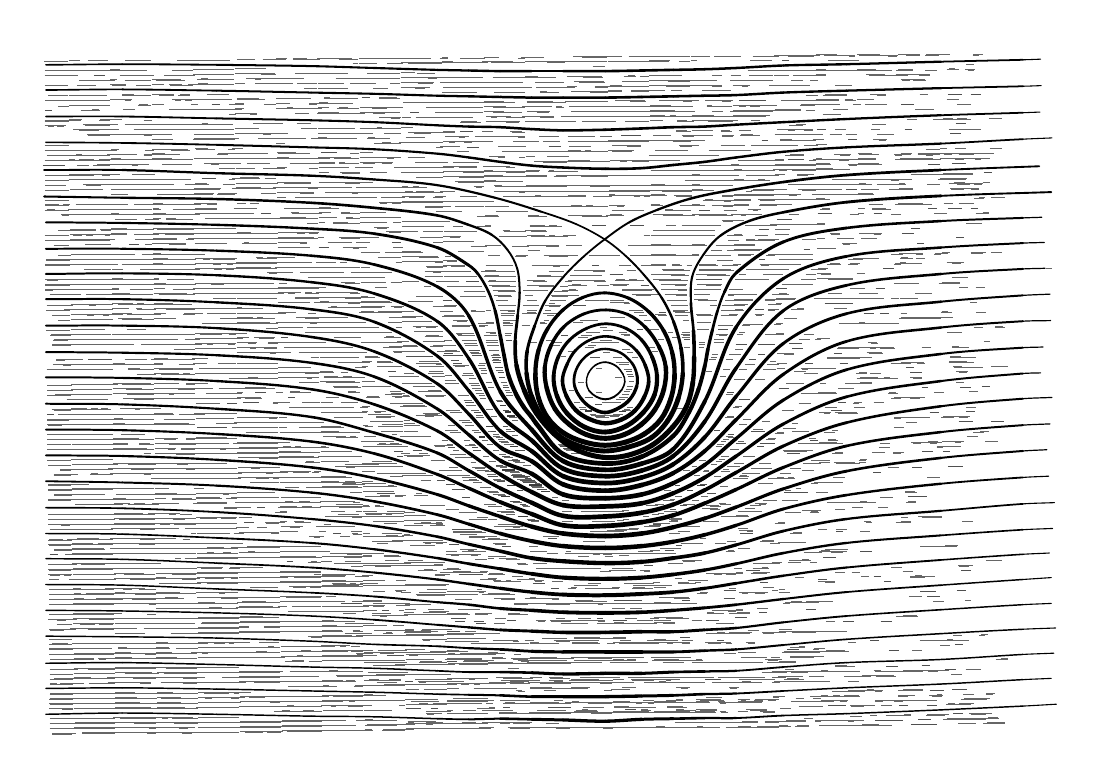
\begin{tikzpicture}[x=.08mm,y=-.08mm,line cap=round,line join=round]
\path[use as bounding box] (0,0) rectangle (1680,1150);

% Horizontal lithographic shading, separated from the contour lines.
% Each segment is editable in the same source-coordinate system.
\draw[black!60,line width=0.072mm,line cap=butt]
  (1251,43) -- (1285,43)
  (1317,43) -- (1353,43)
  (1382,43) -- (1416,43)
  (1426,43) -- (1464,43)
  (1501,43) -- (1517,43)
  (1185,44) -- (1258,44)
  (1264,44) -- (1314,44)
  (1320,44) -- (1381,44)
  (1395,44) -- (1417,44)
  (1425,44) -- (1447,44)
  (1500,44) -- (1511,44)
  (987,45) -- (1045,45)
  (1053,45) -- (1084,45)
  (1090,45) -- (1133,45)
  (1151,45) -- (1192,45)
  (1207,45) -- (1248,45)
  (1304,45) -- (1314,45)
  (1366,45) -- (1380,45)
  (866,46) -- (944,46)
  (954,46) -- (992,46)
  (999,46) -- (1052,46)
  (1091,46) -- (1118,46)
  (658,47) -- (667,47)
  (724,47) -- (749,47)
  (783,47) -- (819,47)
  (880,47) -- (920,47)
  (592,48) -- (641,48)
  (654,48) -- (668,48)
  (686,48) -- (726,48)
  (779,48) -- (789,48)
  (394,49) -- (411,49)
  (421,49) -- (443,49)
  (460,49) -- (515,49)
  (526,49) -- (596,49)
  (606,49) -- (640,49)
  (332,50) -- (361,50)
  (373,50) -- (410,50)
  (421,50) -- (464,50)
  (494,50) -- (525,50)
  (155,51) -- (167,51)
  (259,51) -- (321,51)
  (1271,51) -- (1319,51)
  (65,52) -- (83,52)
  (95,52) -- (127,52)
  (157,52) -- (196,52)
  (237,52) -- (262,52)
  (987,52) -- (1019,52)
  (1053,52) -- (1063,52)
  (1147,52) -- (1181,52)
  (26,53) -- (64,53)
  (855,53) -- (904,53)
  (921,53) -- (1018,53)
  (1034,53) -- (1052,53)
  (658,54) -- (675,54)
  (722,54) -- (771,54)
  (790,54) -- (920,54)
  (592,55) -- (730,55)
  (736,55) -- (789,55)
  (825,55) -- (853,55)
  (526,56) -- (555,56)
  (571,56) -- (596,56)
  (604,56) -- (657,56)
  (516,57) -- (525,57)
  (1490,58) -- (1503,58)
  (897,62) -- (916,62)
  (329,65) -- (378,65)
  (1463,65) -- (1472,65)
  (131,66) -- (147,66)
  (263,66) -- (328,66)
  (1252,66) -- (1268,66)
  (1317,66) -- (1346,66)
  (1382,66) -- (1406,66)
  (1459,66) -- (1478,66)
  (1488,66) -- (1504,66)
  (65,67) -- (190,67);
\draw[black!60,line width=0.072mm,line cap=butt]
  (229,67) -- (262,67)
  (1185,67) -- (1372,67)
  (1379,67) -- (1405,67)
  (1425,67) -- (1444,67)
  (1492,67) -- (1503,67)
  (27,68) -- (66,68)
  (87,68) -- (130,68)
  (1143,68) -- (1200,68)
  (1206,68) -- (1219,68)
  (1226,68) -- (1250,68)
  (1301,68) -- (1316,68)
  (1345,68) -- (1371,68)
  (592,71) -- (615,71)
  (424,72) -- (436,72)
  (460,72) -- (500,72)
  (539,72) -- (591,72)
  (618,72) -- (647,72)
  (329,73) -- (393,73)
  (424,73) -- (459,73)
  (476,73) -- (509,73)
  (263,74) -- (328,74)
  (370,74) -- (394,74)
  (1251,74) -- (1268,74)
  (1331,74) -- (1361,74)
  (1378,74) -- (1432,74)
  (65,75) -- (80,75)
  (146,75) -- (201,75)
  (217,75) -- (266,75)
  (1119,75) -- (1131,75)
  (1145,75) -- (1172,75)
  (1185,75) -- (1208,75)
  (1215,75) -- (1268,75)
  (1335,75) -- (1398,75)
  (1415,75) -- (1432,75)
  (27,76) -- (66,76)
  (187,76) -- (196,76)
  (953,76) -- (964,76)
  (987,76) -- (1038,76)
  (1086,76) -- (1102,76)
  (1116,76) -- (1133,76)
  (1146,76) -- (1184,76)
  (1227,76) -- (1246,76)
  (790,77) -- (810,77)
  (856,77) -- (912,77)
  (946,77) -- (965,77)
  (972,77) -- (986,77)
  (658,78) -- (720,78)
  (738,78) -- (838,78)
  (881,78) -- (913,78)
  (592,79) -- (723,79)
  (771,79) -- (789,79)
  (395,80) -- (439,80)
  (489,80) -- (591,80)
  (635,80) -- (650,80)
  (275,81) -- (287,81)
  (347,81) -- (394,81)
  (404,81) -- (416,81)
  (423,81) -- (439,81)
  (495,81) -- (525,81)
  (131,82) -- (142,82)
  (197,82) -- (244,82)
  (269,82) -- (328,82)
  (361,82) -- (370,82)
  (1386,82) -- (1425,82)
  (82,83) -- (139,83)
  (154,83) -- (196,83)
  (203,83) -- (249,83)
  (1119,83) -- (1131,83)
  (1153,83) -- (1173,83)
  (1212,83) -- (1231,83)
  (1242,83) -- (1254,83)
  (1388,83) -- (1400,83)
  (1406,83) -- (1426,83)
  (100,84) -- (112,84)
  (987,84) -- (1095,84);
\draw[black!60,line width=0.072mm,line cap=butt]
  (1115,84) -- (1184,84)
  (867,85) -- (915,85)
  (944,85) -- (986,85)
  (1016,85) -- (1052,85)
  (658,86) -- (786,86)
  (806,86) -- (851,86)
  (876,86) -- (916,86)
  (592,87) -- (645,87)
  (655,87) -- (723,87)
  (765,87) -- (785,87)
  (395,88) -- (422,88)
  (428,88) -- (449,88)
  (461,88) -- (502,88)
  (512,88) -- (553,88)
  (575,88) -- (591,88)
  (619,88) -- (643,88)
  (270,89) -- (287,89)
  (329,89) -- (345,89)
  (361,89) -- (398,89)
  (428,89) -- (460,89)
  (512,89) -- (524,89)
  (131,90) -- (156,90)
  (197,90) -- (217,90)
  (225,90) -- (245,90)
  (255,90) -- (328,90)
  (78,91) -- (108,91)
  (134,91) -- (156,91)
  (172,91) -- (196,91)
  (226,91) -- (262,91)
  (1185,91) -- (1242,91)
  (1282,91) -- (1308,91)
  (27,92) -- (64,92)
  (924,92) -- (943,92)
  (987,92) -- (1102,92)
  (1119,92) -- (1146,92)
  (1177,92) -- (1198,92)
  (1204,92) -- (1240,92)
  (856,93) -- (872,93)
  (900,93) -- (986,93)
  (1014,93) -- (1052,93)
  (1086,93) -- (1103,93)
  (1134,93) -- (1143,93)
  (660,94) -- (697,94)
  (720,94) -- (800,94)
  (807,94) -- (869,94)
  (900,94) -- (921,94)
  (592,95) -- (639,95)
  (661,95) -- (723,95)
  (758,95) -- (789,95)
  (827,95) -- (847,95)
  (461,96) -- (509,96)
  (549,96) -- (572,96)
  (615,96) -- (630,96)
  (439,97) -- (460,97)
  (491,97) -- (509,97)
  (922,100) -- (943,100)
  (958,100) -- (1012,100)
  (1021,100) -- (1039,100)
  (1071,100) -- (1117,100)
  (813,101) -- (824,101)
  (863,101) -- (943,101)
  (958,101) -- (987,101)
  (658,102) -- (713,102)
  (740,102) -- (790,102)
  (813,102) -- (843,102)
  (893,102) -- (921,102)
  (697,103) -- (714,103)
  (284,105) -- (296,105)
  (150,106) -- (168,106)
  (197,106) -- (233,106)
  (242,106) -- (258,106)
  (285,106) -- (319,106)
  (1265,106) -- (1301,106)
  (1338,106) -- (1362,106)
  (1416,106) -- (1430,106);
\draw[black!60,line width=0.072mm,line cap=butt]
  (65,107) -- (126,107)
  (150,107) -- (196,107)
  (209,107) -- (233,107)
  (239,107) -- (258,107)
  (1235,107) -- (1254,107)
  (1262,107) -- (1301,107)
  (1348,107) -- (1363,107)
  (32,108) -- (64,108)
  (471,111) -- (480,111)
  (558,111) -- (586,111)
  (332,112) -- (367,112)
  (395,112) -- (450,112)
  (470,112) -- (524,112)
  (558,112) -- (591,112)
  (265,113) -- (325,113)
  (333,113) -- (376,113)
  (1317,113) -- (1326,113)
  (1459,113) -- (1478,113)
  (131,114) -- (165,114)
  (229,114) -- (324,114)
  (1251,114) -- (1288,114)
  (1297,114) -- (1310,114)
  (1317,114) -- (1344,114)
  (1466,114) -- (1476,114)
  (28,115) -- (43,115)
  (66,115) -- (130,115)
  (154,115) -- (164,115)
  (234,115) -- (244,115)
  (250,115) -- (261,115)
  (1054,115) -- (1064,115)
  (1196,115) -- (1288,115)
  (1297,115) -- (1315,115)
  (28,116) -- (65,116)
  (933,116) -- (980,116)
  (1003,116) -- (1065,116)
  (1076,116) -- (1120,116)
  (724,117) -- (756,117)
  (792,117) -- (834,117)
  (853,117) -- (921,117)
  (957,117) -- (981,117)
  (1040,117) -- (1055,117)
  (1102,117) -- (1117,117)
  (658,118) -- (773,118)
  (793,118) -- (855,118)
  (463,119) -- (476,119)
  (596,119) -- (657,119)
  (329,120) -- (343,120)
  (395,120) -- (416,120)
  (447,120) -- (517,120)
  (320,121) -- (343,121)
  (375,121) -- (395,121)
  (447,121) -- (459,121)
  (1476,121) -- (1497,121)
  (176,122) -- (191,122)
  (197,122) -- (217,122)
  (260,122) -- (270,122)
  (1227,122) -- (1290,122)
  (1311,122) -- (1323,122)
  (1329,122) -- (1364,122)
  (66,123) -- (130,123)
  (175,123) -- (196,123)
  (988,123) -- (1022,123)
  (1078,123) -- (1087,123)
  (1119,123) -- (1190,123)
  (1226,123) -- (1250,123)
  (48,124) -- (65,124)
  (862,124) -- (890,124)
  (922,124) -- (1057,124)
  (1078,124) -- (1118,124)
  (1130,124) -- (1140,124)
  (1147,124) -- (1162,124)
  (724,125) -- (760,125)
  (785,125) -- (832,125)
  (839,125) -- (848,125)
  (860,125) -- (923,125);
\draw[black!60,line width=0.072mm,line cap=butt]
  (968,125) -- (981,125)
  (634,126) -- (723,126)
  (739,126) -- (790,126)
  (839,126) -- (851,126)
  (411,127) -- (422,127)
  (461,127) -- (478,127)
  (494,127) -- (508,127)
  (527,127) -- (596,127)
  (633,127) -- (657,127)
  (329,128) -- (343,128)
  (395,128) -- (467,128)
  (491,128) -- (526,128)
  (547,128) -- (570,128)
  (263,129) -- (341,129)
  (102,130) -- (114,130)
  (151,130) -- (171,130)
  (225,130) -- (262,130)
  (318,130) -- (327,130)
  (1186,130) -- (1227,130)
  (1279,130) -- (1303,130)
  (1409,130) -- (1439,130)
  (84,131) -- (115,131)
  (988,131) -- (1027,131)
  (1120,131) -- (1227,131)
  (1235,131) -- (1250,131)
  (864,132) -- (875,132)
  (922,132) -- (1059,132)
  (1087,132) -- (1104,132)
  (1115,132) -- (1183,132)
  (724,133) -- (756,133)
  (793,133) -- (829,133)
  (863,133) -- (923,133)
  (950,133) -- (987,133)
  (655,134) -- (723,134)
  (739,134) -- (785,134)
  (808,134) -- (828,134)
  (461,135) -- (494,135)
  (527,135) -- (591,135)
  (647,135) -- (657,135)
  (329,136) -- (364,136)
  (424,136) -- (447,136)
  (460,136) -- (535,136)
  (549,136) -- (568,136)
  (320,137) -- (330,137)
  (353,137) -- (364,137)
  (1262,138) -- (1291,138)
  (988,139) -- (1012,139)
  (1019,139) -- (1029,139)
  (1054,139) -- (1090,139)
  (1120,139) -- (1178,139)
  (870,140) -- (893,140)
  (922,140) -- (1172,140)
  (728,141) -- (767,141)
  (785,141) -- (835,141)
  (847,141) -- (923,141)
  (949,141) -- (978,141)
  (594,142) -- (608,142)
  (616,142) -- (707,142)
  (736,142) -- (745,142)
  (759,142) -- (789,142)
  (814,142) -- (835,142)
  (558,143) -- (593,143)
  (616,143) -- (658,143)
  (576,144) -- (591,144)
  (1453,144) -- (1469,144)
  (1475,144) -- (1491,144)
  (1526,144) -- (1547,144)
  (1438,145) -- (1498,145)
  (66,146) -- (86,146)
  (115,146) -- (150,146)
  (1396,146) -- (1412,146)
  (1439,146) -- (1448,146)
  (1457,146) -- (1467,146)
  (27,147) -- (85,147)
  (114,147) -- (131,147);
\draw[black!60,line width=0.072mm,line cap=butt]
  (184,147) -- (197,147)
  (988,147) -- (1009,147)
  (1031,147) -- (1047,147)
  (1054,147) -- (1127,147)
  (1148,147) -- (1162,147)
  (27,148) -- (65,148)
  (790,148) -- (799,148)
  (856,148) -- (871,148)
  (880,148) -- (914,148)
  (921,148) -- (934,148)
  (949,148) -- (987,148)
  (1031,148) -- (1058,148)
  (1080,148) -- (1119,148)
  (688,149) -- (713,149)
  (727,149) -- (781,149)
  (791,149) -- (867,149)
  (884,149) -- (921,149)
  (687,150) -- (719,150)
  (760,150) -- (780,150)
  (395,151) -- (405,151)
  (276,152) -- (286,152)
  (358,152) -- (394,152)
  (427,152) -- (449,152)
  (132,153) -- (141,153)
  (198,153) -- (251,153)
  (263,153) -- (326,153)
  (1341,153) -- (1354,153)
  (88,154) -- (143,154)
  (154,154) -- (221,154)
  (227,154) -- (262,154)
  (1219,154) -- (1236,154)
  (1341,154) -- (1362,154)
  (27,155) -- (61,155)
  (91,155) -- (131,155)
  (1209,155) -- (1231,155)
  (32,156) -- (41,156)
  (47,156) -- (57,156)
  (554,158) -- (563,158)
  (593,158) -- (611,158)
  (434,159) -- (447,159)
  (461,159) -- (519,159)
  (527,159) -- (592,159)
  (329,160) -- (367,160)
  (435,160) -- (460,160)
  (508,160) -- (519,160)
  (132,161) -- (145,161)
  (198,161) -- (328,161)
  (1462,161) -- (1514,161)
  (72,162) -- (145,162)
  (168,162) -- (197,162)
  (206,162) -- (226,162)
  (233,162) -- (263,162)
  (1190,162) -- (1247,162)
  (1282,162) -- (1299,162)
  (1339,162) -- (1353,162)
  (1464,162) -- (1483,162)
  (1497,162) -- (1512,162)
  (82,163) -- (114,163)
  (1030,163) -- (1047,163)
  (1054,163) -- (1088,163)
  (1101,163) -- (1115,163)
  (1129,163) -- (1148,163)
  (1207,163) -- (1218,163)
  (1232,163) -- (1247,163)
  (1029,164) -- (1053,164)
  (1101,164) -- (1118,164)
  (659,165) -- (678,165)
  (722,165) -- (738,165)
  (766,165) -- (785,165)
  (604,166) -- (678,166)
  (769,166) -- (789,166)
  (395,167) -- (414,167)
  (461,167) -- (549,167)
  (566,167) -- (592,167)
  (614,167) -- (640,167);
\draw[black!60,line width=0.072mm,line cap=butt]
  (329,168) -- (396,168)
  (403,168) -- (413,168)
  (502,168) -- (526,168)
  (198,169) -- (229,169)
  (264,169) -- (328,169)
  (374,169) -- (387,169)
  (1252,169) -- (1263,169)
  (1273,169) -- (1290,169)
  (94,170) -- (198,170)
  (206,170) -- (229,170)
  (1132,170) -- (1152,170)
  (1186,170) -- (1263,170)
  (1273,170) -- (1293,170)
  (1299,170) -- (1316,170)
  (1349,170) -- (1375,170)
  (95,171) -- (131,171)
  (184,171) -- (197,171)
  (993,171) -- (1022,171)
  (1038,171) -- (1088,171)
  (1102,171) -- (1122,171)
  (1131,171) -- (1163,171)
  (725,172) -- (752,172)
  (814,172) -- (830,172)
  (857,172) -- (901,172)
  (909,172) -- (928,172)
  (1040,172) -- (1058,172)
  (1102,172) -- (1119,172)
  (663,173) -- (700,173)
  (710,173) -- (790,173)
  (812,173) -- (844,173)
  (875,173) -- (885,173)
  (910,173) -- (921,173)
  (461,174) -- (475,174)
  (540,174) -- (551,174)
  (600,174) -- (630,174)
  (684,174) -- (694,174)
  (779,174) -- (789,174)
  (395,175) -- (442,175)
  (450,175) -- (523,175)
  (539,175) -- (575,175)
  (264,176) -- (335,176)
  (366,176) -- (394,176)
  (510,176) -- (523,176)
  (198,177) -- (231,177)
  (263,177) -- (329,177)
  (1194,177) -- (1214,177)
  (1246,177) -- (1264,177)
  (1342,177) -- (1364,177)
  (998,178) -- (1007,178)
  (1194,178) -- (1251,178)
  (1351,178) -- (1363,178)
  (922,179) -- (1075,179)
  (1209,179) -- (1224,179)
  (725,180) -- (736,180)
  (791,180) -- (811,180)
  (818,180) -- (830,180)
  (857,180) -- (987,180)
  (1024,180) -- (1053,180)
  (659,181) -- (738,181)
  (771,181) -- (811,181)
  (819,181) -- (845,181)
  (901,181) -- (920,181)
  (563,182) -- (577,182)
  (589,182) -- (660,182)
  (669,182) -- (679,182)
  (693,182) -- (706,182)
  (395,183) -- (409,183)
  (550,183) -- (592,183)
  (1252,185) -- (1269,185)
  (1054,186) -- (1063,186)
  (1121,186) -- (1139,186)
  (1151,186) -- (1223,186)
  (1233,186) -- (1255,186)
  (27,187) -- (65,187)
  (928,187) -- (973,187);
\draw[black!60,line width=0.072mm,line cap=butt]
  (1034,187) -- (1065,187)
  (1100,187) -- (1138,187)
  (1149,187) -- (1185,187)
  (860,188) -- (895,188)
  (951,188) -- (973,188)
  (1036,188) -- (1054,188)
  (655,189) -- (687,189)
  (747,189) -- (791,189)
  (649,190) -- (660,190)
  (1527,191) -- (1547,191)
  (266,192) -- (286,192)
  (325,192) -- (342,192)
  (1449,192) -- (1459,192)
  (1472,192) -- (1490,192)
  (1527,192) -- (1543,192)
  (132,193) -- (145,193)
  (198,193) -- (255,193)
  (267,193) -- (298,193)
  (318,193) -- (329,193)
  (1426,193) -- (1448,193)
  (66,194) -- (142,194)
  (186,194) -- (201,194)
  (228,194) -- (258,194)
  (996,194) -- (1027,194)
  (1120,194) -- (1148,194)
  (27,195) -- (65,195)
  (857,195) -- (878,195)
  (884,195) -- (895,195)
  (922,195) -- (962,195)
  (998,195) -- (1048,195)
  (1081,195) -- (1123,195)
  (753,196) -- (778,196)
  (791,196) -- (921,196)
  (928,196) -- (960,196)
  (681,197) -- (700,197)
  (753,197) -- (793,197)
  (816,197) -- (841,197)
  (396,198) -- (426,198)
  (527,198) -- (549,198)
  (330,199) -- (382,199)
  (397,199) -- (448,199)
  (512,199) -- (526,199)
  (1449,199) -- (1478,199)
  (1503,199) -- (1534,199)
  (198,200) -- (218,200)
  (302,200) -- (332,200)
  (340,200) -- (353,200)
  (363,200) -- (382,200)
  (1318,200) -- (1341,200)
  (1386,200) -- (1404,200)
  (1413,200) -- (1514,200)
  (77,201) -- (86,201)
  (126,201) -- (174,201)
  (184,201) -- (242,201)
  (301,201) -- (318,201)
  (1211,201) -- (1232,201)
  (1280,201) -- (1307,201)
  (1319,201) -- (1351,201)
  (1376,201) -- (1403,201)
  (1413,201) -- (1448,201)
  (1454,201) -- (1467,201)
  (1478,201) -- (1502,201)
  (30,202) -- (46,202)
  (52,202) -- (131,202)
  (184,202) -- (197,202)
  (988,202) -- (1035,202)
  (1054,202) -- (1095,202)
  (1203,202) -- (1232,202)
  (1290,202) -- (1305,202)
  (1377,202) -- (1388,202)
  (1426,202) -- (1438,202)
  (30,203) -- (65,203)
  (986,203) -- (1097,203)
  (732,204) -- (757,204)
  (791,204) -- (806,204);
\draw[black!60,line width=0.072mm,line cap=butt]
  (825,204) -- (859,204)
  (603,205) -- (630,205)
  (747,205) -- (757,205)
  (780,205) -- (790,205)
  (396,206) -- (415,206)
  (461,206) -- (513,206)
  (527,206) -- (592,206)
  (330,207) -- (480,207)
  (487,207) -- (526,207)
  (571,207) -- (581,207)
  (1513,207) -- (1527,207)
  (132,208) -- (148,208)
  (198,208) -- (229,208)
  (264,208) -- (330,208)
  (367,208) -- (395,208)
  (1252,208) -- (1261,208)
  (1318,208) -- (1347,208)
  (1385,208) -- (1438,208)
  (1448,208) -- (1525,208)
  (66,209) -- (75,209)
  (81,209) -- (106,209)
  (114,209) -- (263,209)
  (1186,209) -- (1200,209)
  (1246,209) -- (1347,209)
  (1377,209) -- (1450,209)
  (1472,209) -- (1486,209)
  (1504,209) -- (1513,209)
  (27,210) -- (131,210)
  (988,210) -- (1029,210)
  (1134,210) -- (1200,210)
  (1241,210) -- (1251,210)
  (1288,210) -- (1304,210)
  (28,211) -- (65,211)
  (857,211) -- (893,211)
  (924,211) -- (1035,211)
  (1128,211) -- (1163,211)
  (1176,211) -- (1185,211)
  (804,212) -- (925,212)
  (940,212) -- (951,212)
  (960,212) -- (987,212)
  (616,213) -- (668,213)
  (676,213) -- (716,213)
  (818,213) -- (856,213)
  (462,214) -- (488,214)
  (495,214) -- (504,214)
  (527,214) -- (580,214)
  (615,214) -- (658,214)
  (330,215) -- (339,215)
  (348,215) -- (384,215)
  (416,215) -- (488,215)
  (495,215) -- (526,215)
  (532,215) -- (552,215)
  (562,215) -- (578,215)
  (280,216) -- (335,216)
  (362,216) -- (384,216)
  (1252,216) -- (1273,216)
  (1318,216) -- (1351,216)
  (110,217) -- (193,217)
  (214,217) -- (261,217)
  (291,217) -- (303,217)
  (1117,217) -- (1130,217)
  (1186,217) -- (1276,217)
  (1303,217) -- (1356,217)
  (79,218) -- (98,218)
  (104,218) -- (131,218)
  (165,218) -- (175,218)
  (1077,218) -- (1251,218)
  (1304,218) -- (1316,218)
  (1066,219) -- (1126,219)
  (1140,219) -- (1170,219)
  (659,220) -- (713,220)
  (723,220) -- (766,220)
  (588,221) -- (677,221)
  (684,221) -- (714,221)
  (760,221) -- (774,221);
\draw[black!60,line width=0.072mm,line cap=butt]
  (396,222) -- (412,222)
  (462,222) -- (510,222)
  (520,222) -- (548,222)
  (582,222) -- (598,222)
  (626,222) -- (640,222)
  (330,223) -- (361,223)
  (374,223) -- (409,223)
  (446,223) -- (461,223)
  (304,224) -- (329,224)
  (376,224) -- (391,224)
  (1252,224) -- (1278,224)
  (1122,225) -- (1134,225)
  (1183,225) -- (1306,225)
  (999,226) -- (1187,226)
  (1193,226) -- (1205,226)
  (1213,226) -- (1251,226)
  (725,227) -- (739,227)
  (791,227) -- (813,227)
  (827,227) -- (836,227)
  (989,227) -- (1008,227)
  (1016,227) -- (1053,227)
  (1061,227) -- (1071,227)
  (1095,227) -- (1119,227)
  (659,228) -- (812,228)
  (826,228) -- (873,228)
  (593,229) -- (661,229)
  (691,229) -- (724,229)
  (759,229) -- (790,229)
  (462,230) -- (479,230)
  (496,230) -- (527,230)
  (543,230) -- (571,230)
  (499,231) -- (527,231)
  (1453,231) -- (1500,231)
  (132,232) -- (147,232)
  (1428,232) -- (1500,232)
  (66,233) -- (147,233)
  (166,233) -- (202,233)
  (1054,233) -- (1067,233)
  (1186,233) -- (1202,233)
  (1222,233) -- (1248,233)
  (1403,233) -- (1448,233)
  (28,234) -- (105,234)
  (118,234) -- (131,234)
  (923,234) -- (983,234)
  (989,234) -- (1129,234)
  (1141,234) -- (1192,234)
  (1222,234) -- (1239,234)
  (725,235) -- (754,235)
  (791,235) -- (824,235)
  (838,235) -- (992,235)
  (998,235) -- (1009,235)
  (1019,235) -- (1058,235)
  (1083,235) -- (1119,235)
  (1143,235) -- (1162,235)
  (659,236) -- (824,236)
  (835,236) -- (856,236)
  (879,236) -- (922,236)
  (617,237) -- (659,237)
  (685,237) -- (724,237)
  (337,238) -- (368,238)
  (325,239) -- (369,239)
  (376,239) -- (395,239)
  (1449,239) -- (1491,239)
  (132,240) -- (165,240)
  (171,240) -- (184,240)
  (198,240) -- (259,240)
  (319,240) -- (329,240)
  (1290,240) -- (1311,240)
  (1320,240) -- (1357,240)
  (1364,240) -- (1374,240)
  (1384,240) -- (1404,240)
  (1445,240) -- (1489,240)
  (65,241) -- (197,241)
  (226,241) -- (260,241)
  (1122,241) -- (1137,241);
\draw[black!60,line width=0.072mm,line cap=butt]
  (1160,241) -- (1170,241)
  (1277,241) -- (1383,241)
  (28,242) -- (66,242)
  (1045,242) -- (1178,242)
  (1370,242) -- (1383,242)
  (725,243) -- (743,243)
  (1043,243) -- (1063,243)
  (1071,243) -- (1119,243)
  (1129,243) -- (1142,243)
  (678,244) -- (787,244)
  (683,245) -- (724,245)
  (396,246) -- (449,246)
  (462,246) -- (549,246)
  (1470,246) -- (1488,246)
  (1516,246) -- (1528,246)
  (266,247) -- (285,247)
  (330,247) -- (398,247)
  (407,247) -- (449,247)
  (504,247) -- (527,247)
  (1319,247) -- (1331,247)
  (1384,247) -- (1393,247)
  (1462,247) -- (1516,247)
  (132,248) -- (162,248)
  (198,248) -- (231,248)
  (250,248) -- (288,248)
  (310,248) -- (329,248)
  (1238,248) -- (1341,248)
  (1348,248) -- (1394,248)
  (1428,248) -- (1449,248)
  (1475,248) -- (1496,248)
  (1503,248) -- (1515,248)
  (88,249) -- (197,249)
  (218,249) -- (233,249)
  (249,249) -- (263,249)
  (990,249) -- (1012,249)
  (1055,249) -- (1068,249)
  (1207,249) -- (1317,249)
  (1327,249) -- (1341,249)
  (1348,249) -- (1383,249)
  (28,250) -- (61,250)
  (92,250) -- (116,250)
  (857,250) -- (876,250)
  (923,250) -- (1120,250)
  (740,251) -- (753,251)
  (791,251) -- (987,251)
  (1023,251) -- (1054,251)
  (1076,251) -- (1119,251)
  (594,252) -- (604,252)
  (611,252) -- (622,252)
  (708,252) -- (724,252)
  (742,252) -- (856,252)
  (893,252) -- (924,252)
  (462,253) -- (473,253)
  (479,253) -- (488,253)
  (528,253) -- (564,253)
  (570,253) -- (634,253)
  (712,253) -- (721,253)
  (330,254) -- (371,254)
  (389,254) -- (515,254)
  (521,254) -- (592,254)
  (264,255) -- (307,255)
  (325,255) -- (395,255)
  (445,255) -- (461,255)
  (1384,255) -- (1406,255)
  (1465,255) -- (1511,255)
  (133,256) -- (306,256)
  (1228,256) -- (1237,256)
  (1252,256) -- (1293,256)
  (1323,256) -- (1352,256)
  (1368,256) -- (1406,256)
  (1466,256) -- (1487,256)
  (1498,256) -- (1510,256)
  (67,257) -- (119,257)
  (145,257) -- (197,257)
  (234,257) -- (260,257);
\draw[black!60,line width=0.072mm,line cap=butt]
  (1055,257) -- (1072,257)
  (1152,257) -- (1206,257)
  (1223,257) -- (1293,257)
  (1342,257) -- (1351,257)
  (1367,257) -- (1383,257)
  (28,258) -- (66,258)
  (923,258) -- (1089,258)
  (1148,258) -- (1185,258)
  (1230,258) -- (1251,258)
  (740,259) -- (758,259)
  (791,259) -- (838,259)
  (847,259) -- (988,259)
  (1007,259) -- (1054,259)
  (1140,259) -- (1150,259)
  (599,260) -- (611,260)
  (617,260) -- (645,260)
  (655,260) -- (679,260)
  (742,260) -- (871,260)
  (892,260) -- (922,260)
  (528,261) -- (660,261)
  (780,261) -- (790,261)
  (396,262) -- (454,262)
  (472,262) -- (593,262)
  (264,263) -- (296,263)
  (302,263) -- (333,263)
  (371,263) -- (395,263)
  (433,263) -- (454,263)
  (515,263) -- (525,263)
  (1318,263) -- (1342,263)
  (133,264) -- (159,264)
  (206,264) -- (295,264)
  (301,264) -- (329,264)
  (1186,264) -- (1228,264)
  (1245,264) -- (1343,264)
  (233,265) -- (260,265)
  (923,265) -- (932,265)
  (989,265) -- (1012,265)
  (1121,265) -- (1228,265)
  (1257,265) -- (1268,265)
  (1285,265) -- (1295,265)
  (1301,265) -- (1316,265)
  (806,266) -- (815,266)
  (857,266) -- (886,266)
  (923,266) -- (1015,266)
  (1026,266) -- (1054,266)
  (1103,266) -- (1185,266)
  (1208,266) -- (1221,266)
  (689,267) -- (708,267)
  (761,267) -- (783,267)
  (789,267) -- (886,267)
  (898,267) -- (927,267)
  (962,267) -- (972,267)
  (978,267) -- (988,267)
  (1029,267) -- (1054,267)
  (1103,267) -- (1120,267)
  (594,268) -- (631,268)
  (646,268) -- (664,268)
  (687,268) -- (714,268)
  (755,268) -- (790,268)
  (811,268) -- (856,268)
  (462,269) -- (498,269)
  (528,269) -- (555,269)
  (561,269) -- (599,269)
  (606,269) -- (629,269)
  (644,269) -- (659,269)
  (396,270) -- (410,270)
  (425,270) -- (527,270)
  (563,270) -- (593,270)
  (1511,270) -- (1520,270)
  (1529,270) -- (1552,270)
  (1252,271) -- (1266,271)
  (1503,271) -- (1518,271)
  (1188,272) -- (1241,272)
  (1249,272) -- (1274,272)
  (1076,273) -- (1088,273);
\draw[black!60,line width=0.072mm,line cap=butt]
  (1122,273) -- (1149,273)
  (1160,273) -- (1260,273)
  (27,274) -- (66,274)
  (1072,274) -- (1149,274)
  (1162,274) -- (1186,274)
  (660,275) -- (700,275)
  (725,275) -- (741,275)
  (1105,275) -- (1117,275)
  (594,276) -- (724,276)
  (558,277) -- (660,277)
  (560,278) -- (571,278)
  (579,278) -- (592,278)
  (1457,278) -- (1469,278)
  (199,279) -- (215,279)
  (264,279) -- (301,279)
  (333,279) -- (347,279)
  (353,279) -- (367,279)
  (1382,279) -- (1422,279)
  (1454,279) -- (1469,279)
  (1478,279) -- (1503,279)
  (87,280) -- (103,280)
  (113,280) -- (160,280)
  (169,280) -- (275,280)
  (284,280) -- (301,280)
  (1188,280) -- (1198,280)
  (1335,280) -- (1358,280)
  (1377,280) -- (1435,280)
  (28,281) -- (50,281)
  (56,281) -- (67,281)
  (76,281) -- (132,281)
  (170,281) -- (198,281)
  (989,281) -- (1004,281)
  (1055,281) -- (1068,281)
  (1122,281) -- (1145,281)
  (1162,281) -- (1213,281)
  (28,282) -- (66,282)
  (862,282) -- (880,282)
  (886,282) -- (898,282)
  (923,282) -- (949,282)
  (989,282) -- (1008,282)
  (1035,282) -- (1075,282)
  (1086,282) -- (1145,282)
  (1161,282) -- (1190,282)
  (726,283) -- (764,283)
  (803,283) -- (922,283)
  (936,283) -- (947,283)
  (1104,283) -- (1119,283)
  (631,284) -- (672,284)
  (679,284) -- (725,284)
  (836,284) -- (856,284)
  (462,285) -- (482,285)
  (630,285) -- (659,285)
  (330,286) -- (364,286)
  (407,286) -- (494,286)
  (199,287) -- (208,287)
  (265,287) -- (300,287)
  (327,287) -- (364,287)
  (1261,287) -- (1274,287)
  (1318,287) -- (1329,287)
  (1341,287) -- (1362,287)
  (73,288) -- (85,288)
  (133,288) -- (189,288)
  (199,288) -- (211,288)
  (230,288) -- (300,288)
  (1258,288) -- (1274,288)
  (1340,288) -- (1371,288)
  (30,289) -- (43,289)
  (64,289) -- (132,289)
  (171,289) -- (198,289)
  (247,289) -- (256,289)
  (1012,289) -- (1025,289)
  (1143,289) -- (1164,289)
  (27,290) -- (66,290)
  (927,290) -- (978,290)
  (1012,290) -- (1053,290);
\draw[black!60,line width=0.072mm,line cap=butt]
  (1105,290) -- (1126,290)
  (1151,290) -- (1160,290)
  (660,291) -- (690,291)
  (744,291) -- (795,291)
  (648,292) -- (662,292)
  (669,292) -- (689,292)
  (775,292) -- (790,292)
  (418,293) -- (430,293)
  (462,293) -- (481,293)
  (498,293) -- (512,293)
  (528,293) -- (569,293)
  (1516,293) -- (1526,293)
  (330,294) -- (359,294)
  (419,294) -- (468,294)
  (498,294) -- (527,294)
  (1450,294) -- (1460,294)
  (1505,294) -- (1526,294)
  (133,295) -- (145,295)
  (199,295) -- (220,295)
  (265,295) -- (339,295)
  (1318,295) -- (1327,295)
  (1439,295) -- (1460,295)
  (1505,295) -- (1515,295)
  (67,296) -- (98,296)
  (112,296) -- (274,296)
  (1211,296) -- (1225,296)
  (1305,296) -- (1319,296)
  (1371,296) -- (1386,296)
  (53,297) -- (132,297)
  (183,297) -- (198,297)
  (925,297) -- (944,297)
  (992,297) -- (1041,297)
  (1055,297) -- (1110,297)
  (1117,297) -- (1165,297)
  (1208,297) -- (1224,297)
  (54,298) -- (66,298)
  (726,298) -- (746,298)
  (795,298) -- (812,298)
  (857,298) -- (912,298)
  (918,298) -- (947,298)
  (1008,298) -- (1059,298)
  (1065,298) -- (1120,298)
  (1132,298) -- (1141,298)
  (714,299) -- (748,299)
  (794,299) -- (824,299)
  (880,299) -- (922,299)
  (716,300) -- (725,300)
  (400,301) -- (442,301)
  (462,301) -- (491,301)
  (506,301) -- (516,301)
  (528,301) -- (593,301)
  (331,302) -- (461,302)
  (506,302) -- (527,302)
  (199,303) -- (212,303)
  (220,303) -- (235,303)
  (282,303) -- (330,303)
  (374,303) -- (394,303)
  (139,304) -- (174,304)
  (187,304) -- (209,304)
  (220,304) -- (262,304)
  (1121,305) -- (1137,305)
  (1102,306) -- (1135,306)
  (660,307) -- (671,307)
  (1104,307) -- (1120,307)
  (594,308) -- (659,308)
  (462,309) -- (472,309)
  (485,309) -- (508,309)
  (528,309) -- (571,309)
  (580,309) -- (593,309)
  (444,310) -- (461,310)
  (485,310) -- (527,310)
  (1490,310) -- (1515,310)
  (1253,311) -- (1266,311)
  (1179,312) -- (1266,312)
  (1014,313) -- (1030,313);
\draw[black!60,line width=0.072mm,line cap=butt]
  (1038,313) -- (1050,313)
  (1056,313) -- (1100,313)
  (1139,313) -- (1190,313)
  (726,314) -- (735,314)
  (797,314) -- (821,314)
  (828,314) -- (840,314)
  (1038,314) -- (1056,314)
  (1068,314) -- (1099,314)
  (675,315) -- (691,315)
  (713,315) -- (736,315)
  (797,315) -- (849,315)
  (594,316) -- (661,316)
  (837,316) -- (847,316)
  (550,317) -- (574,317)
  (267,318) -- (279,318)
  (555,318) -- (570,318)
  (133,319) -- (157,319)
  (199,319) -- (330,319)
  (67,320) -- (109,320)
  (115,320) -- (200,320)
  (206,320) -- (264,320)
  (1187,320) -- (1211,320)
  (48,321) -- (109,321)
  (116,321) -- (132,321)
  (993,321) -- (1091,321)
  (51,322) -- (66,322)
  (754,322) -- (765,322)
  (789,322) -- (823,322)
  (1012,322) -- (1035,322)
  (1041,322) -- (1060,322)
  (1075,322) -- (1089,322)
  (661,323) -- (714,323)
  (756,323) -- (791,323)
  (799,323) -- (824,323)
  (569,324) -- (620,324)
  (628,324) -- (659,324)
  (333,325) -- (354,325)
  (397,325) -- (463,325)
  (574,325) -- (593,325)
  (265,326) -- (280,326)
  (286,326) -- (315,326)
  (321,326) -- (397,326)
  (428,326) -- (440,326)
  (446,326) -- (461,326)
  (133,327) -- (158,327)
  (199,327) -- (330,327)
  (1273,327) -- (1289,327)
  (1320,327) -- (1357,327)
  (67,328) -- (158,328)
  (169,328) -- (208,328)
  (218,328) -- (264,328)
  (1121,328) -- (1134,328)
  (1187,328) -- (1209,328)
  (1276,328) -- (1289,328)
  (1343,328) -- (1354,328)
  (27,329) -- (66,329)
  (72,329) -- (87,329)
  (93,329) -- (104,329)
  (122,329) -- (131,329)
  (989,329) -- (1091,329)
  (1111,329) -- (1136,329)
  (1155,329) -- (1175,329)
  (792,330) -- (822,330)
  (828,330) -- (837,330)
  (850,330) -- (870,330)
  (978,330) -- (988,330)
  (1002,330) -- (1054,330)
  (1076,330) -- (1091,330)
  (1110,330) -- (1120,330)
  (660,331) -- (688,331)
  (749,331) -- (792,331)
  (799,331) -- (857,331)
  (532,332) -- (546,332)
  (623,332) -- (659,332)
  (670,332) -- (687,332);
\draw[black!60,line width=0.072mm,line cap=butt]
  (397,333) -- (455,333)
  (461,333) -- (471,333)
  (495,333) -- (557,333)
  (331,334) -- (461,334)
  (498,334) -- (527,334)
  (1323,334) -- (1344,334)
  (199,335) -- (237,335)
  (255,335) -- (330,335)
  (1253,335) -- (1266,335)
  (1285,335) -- (1312,335)
  (1326,335) -- (1348,335)
  (67,336) -- (139,336)
  (171,336) -- (237,336)
  (252,336) -- (264,336)
  (1140,336) -- (1154,336)
  (1160,336) -- (1192,336)
  (1230,336) -- (1252,336)
  (28,337) -- (131,337)
  (1112,337) -- (1130,337)
  (1140,337) -- (1186,337)
  (38,338) -- (48,338)
  (660,339) -- (709,339)
  (528,340) -- (544,340)
  (644,340) -- (659,340)
  (343,341) -- (352,341)
  (397,341) -- (444,341)
  (476,341) -- (515,341)
  (522,341) -- (543,341)
  (286,342) -- (295,342)
  (340,342) -- (396,342)
  (433,342) -- (443,342)
  (198,343) -- (251,343)
  (265,343) -- (317,343)
  (1293,343) -- (1316,343)
  (91,344) -- (132,344)
  (186,344) -- (198,344)
  (225,344) -- (251,344)
  (989,344) -- (1021,344)
  (1055,344) -- (1076,344)
  (1121,344) -- (1155,344)
  (1295,344) -- (1306,344)
  (41,345) -- (66,345)
  (859,345) -- (879,345)
  (954,345) -- (1078,345)
  (1092,345) -- (1154,345)
  (726,346) -- (751,346)
  (792,346) -- (844,346)
  (855,346) -- (880,346)
  (953,346) -- (967,346)
  (973,346) -- (989,346)
  (1104,346) -- (1114,346)
  (703,347) -- (729,347)
  (769,347) -- (796,347)
  (823,347) -- (844,347)
  (528,348) -- (539,348)
  (582,348) -- (596,348)
  (397,349) -- (448,349)
  (500,349) -- (527,349)
  (580,349) -- (593,349)
  (516,350) -- (526,350)
  (1253,350) -- (1279,350)
  (1254,351) -- (1284,351)
  (1121,352) -- (1165,352)
  (1085,353) -- (1103,353)
  (1110,353) -- (1163,353)
  (794,354) -- (813,354)
  (1111,354) -- (1120,354)
  (594,355) -- (625,355)
  (683,355) -- (725,355)
  (529,356) -- (559,356)
  (568,356) -- (628,356)
  (1530,356) -- (1546,356)
  (538,357) -- (558,357)
  (567,357) -- (593,357)
  (1451,357) -- (1464,357);
\draw[black!60,line width=0.072mm,line cap=butt]
  (1497,357) -- (1522,357)
  (199,358) -- (211,358)
  (1383,358) -- (1421,358)
  (1440,358) -- (1461,358)
  (1498,358) -- (1516,358)
  (133,359) -- (171,359)
  (182,359) -- (281,359)
  (1187,359) -- (1202,359)
  (1208,359) -- (1246,359)
  (1371,359) -- (1390,359)
  (1410,359) -- (1421,359)
  (1439,359) -- (1450,359)
  (68,360) -- (132,360)
  (161,360) -- (171,360)
  (181,360) -- (198,360)
  (239,360) -- (262,360)
  (990,360) -- (1030,360)
  (1055,360) -- (1066,360)
  (1128,360) -- (1153,360)
  (1175,360) -- (1243,360)
  (1374,360) -- (1384,360)
  (48,361) -- (69,361)
  (858,361) -- (874,361)
  (891,361) -- (917,361)
  (923,361) -- (941,361)
  (956,361) -- (1065,361)
  (1075,361) -- (1116,361)
  (1128,361) -- (1148,361)
  (1172,361) -- (1186,361)
  (731,362) -- (750,362)
  (775,362) -- (794,362)
  (819,362) -- (873,362)
  (892,362) -- (923,362)
  (964,362) -- (989,362)
  (1040,362) -- (1054,362)
  (1104,362) -- (1116,362)
  (594,363) -- (652,363)
  (663,363) -- (672,363)
  (774,363) -- (791,363)
  (827,363) -- (857,363)
  (556,364) -- (593,364)
  (622,364) -- (653,364)
  (363,365) -- (374,365)
  (380,365) -- (424,365)
  (1386,365) -- (1398,365)
  (199,366) -- (223,366)
  (265,366) -- (333,366)
  (364,366) -- (396,366)
  (1310,366) -- (1352,366)
  (1385,366) -- (1405,366)
  (1411,366) -- (1425,366)
  (89,367) -- (100,367)
  (133,367) -- (268,367)
  (278,367) -- (289,367)
  (295,367) -- (329,367)
  (1193,367) -- (1247,367)
  (1302,367) -- (1326,367)
  (29,368) -- (132,368)
  (174,368) -- (198,368)
  (240,368) -- (249,368)
  (1196,368) -- (1219,368)
  (1229,368) -- (1244,368)
  (29,369) -- (67,369)
  (1094,369) -- (1120,369)
  (660,370) -- (681,370)
  (595,371) -- (660,371)
  (666,371) -- (681,371)
  (397,372) -- (419,372)
  (463,372) -- (489,372)
  (584,372) -- (594,372)
  (646,372) -- (659,372)
  (331,373) -- (452,373)
  (458,373) -- (487,373)
  (496,373) -- (507,373)
  (1385,373) -- (1395,373);
\draw[black!60,line width=0.072mm,line cap=butt]
  (1459,373) -- (1487,373)
  (199,374) -- (215,374)
  (265,374) -- (396,374)
  (1274,374) -- (1289,374)
  (1305,374) -- (1321,374)
  (1377,374) -- (1420,374)
  (1468,374) -- (1482,374)
  (68,375) -- (90,375)
  (115,375) -- (143,375)
  (149,375) -- (267,375)
  (294,375) -- (307,375)
  (316,375) -- (326,375)
  (1187,375) -- (1227,375)
  (1269,375) -- (1291,375)
  (1303,375) -- (1318,375)
  (1376,375) -- (1387,375)
  (28,376) -- (133,376)
  (176,376) -- (197,376)
  (990,376) -- (1013,376)
  (1023,376) -- (1035,376)
  (1065,376) -- (1092,376)
  (1119,376) -- (1132,376)
  (1162,376) -- (1226,376)
  (28,377) -- (67,377)
  (733,377) -- (745,377)
  (800,377) -- (809,377)
  (939,377) -- (958,377)
  (973,377) -- (1013,377)
  (1023,377) -- (1038,377)
  (1046,377) -- (1055,377)
  (1066,377) -- (1096,377)
  (1103,377) -- (1128,377)
  (1164,377) -- (1177,377)
  (660,378) -- (694,378)
  (727,378) -- (771,378)
  (800,378) -- (859,378)
  (941,378) -- (950,378)
  (979,378) -- (989,378)
  (633,379) -- (666,379)
  (672,379) -- (694,379)
  (834,379) -- (845,379)
  (463,380) -- (504,380)
  (529,380) -- (544,380)
  (634,380) -- (659,380)
  (331,381) -- (386,381)
  (393,381) -- (528,381)
  (265,382) -- (396,382)
  (1254,382) -- (1271,382)
  (1617,382) -- (1626,382)
  (134,383) -- (152,383)
  (179,383) -- (273,383)
  (296,383) -- (308,383)
  (315,383) -- (328,383)
  (1183,383) -- (1208,383)
  (1243,383) -- (1268,383)
  (90,384) -- (133,384)
  (181,384) -- (198,384)
  (1007,384) -- (1042,384)
  (1065,384) -- (1117,384)
  (1141,384) -- (1188,384)
  (726,385) -- (743,385)
  (868,385) -- (916,385)
  (951,385) -- (965,385)
  (1008,385) -- (1052,385)
  (1065,385) -- (1121,385)
  (661,386) -- (703,386)
  (720,386) -- (774,386)
  (827,386) -- (851,386)
  (898,386) -- (916,386)
  (630,387) -- (670,387)
  (764,387) -- (774,387)
  (397,388) -- (417,388)
  (463,388) -- (502,388)
  (526,388) -- (579,388)
  (644,388) -- (656,388);
\draw[black!60,line width=0.072mm,line cap=butt]
  (380,389) -- (421,389)
  (432,389) -- (472,389)
  (485,389) -- (502,389)
  (513,389) -- (528,389)
  (383,390) -- (396,390)
  (1253,390) -- (1276,390)
  (1316,390) -- (1329,390)
  (1171,391) -- (1199,391)
  (1235,391) -- (1252,391)
  (1259,391) -- (1276,391)
  (990,392) -- (1043,392)
  (1061,392) -- (1109,392)
  (1129,392) -- (1140,392)
  (1168,392) -- (1186,392)
  (726,393) -- (748,393)
  (809,393) -- (830,393)
  (861,393) -- (911,393)
  (1021,393) -- (1050,393)
  (1078,393) -- (1115,393)
  (661,394) -- (714,394)
  (725,394) -- (775,394)
  (809,394) -- (848,394)
  (630,395) -- (660,395)
  (677,395) -- (688,395)
  (463,396) -- (518,396)
  (525,396) -- (568,396)
  (1477,396) -- (1488,396)
  (445,397) -- (462,397)
  (499,397) -- (528,397)
  (1467,397) -- (1493,397)
  (134,398) -- (152,398)
  (200,398) -- (209,398)
  (1253,398) -- (1310,398)
  (68,399) -- (209,399)
  (221,399) -- (264,399)
  (1228,399) -- (1252,399)
  (1271,399) -- (1310,399)
  (28,400) -- (133,400)
  (185,400) -- (195,400)
  (934,400) -- (949,400)
  (955,400) -- (968,400)
  (993,400) -- (1037,400)
  (1123,400) -- (1177,400)
  (30,401) -- (48,401)
  (733,401) -- (743,401)
  (792,401) -- (821,401)
  (857,401) -- (916,401)
  (933,401) -- (979,401)
  (1002,401) -- (1048,401)
  (661,402) -- (684,402)
  (730,402) -- (776,402)
  (802,402) -- (825,402)
  (853,402) -- (864,402)
  (899,402) -- (918,402)
  (595,403) -- (621,403)
  (649,403) -- (683,403)
  (497,404) -- (520,404)
  (529,404) -- (569,404)
  (576,404) -- (594,404)
  (1451,404) -- (1480,404)
  (331,405) -- (391,405)
  (399,405) -- (411,405)
  (503,405) -- (528,405)
  (1385,405) -- (1415,405)
  (1446,405) -- (1480,405)
  (200,406) -- (220,406)
  (265,406) -- (334,406)
  (345,406) -- (391,406)
  (1375,406) -- (1414,406)
  (68,407) -- (85,407)
  (91,407) -- (268,407)
  (291,407) -- (311,407)
  (1197,407) -- (1247,407)
  (28,408) -- (133,408)
  (186,408) -- (199,408);
\draw[black!60,line width=0.072mm,line cap=butt]
  (864,408) -- (878,408)
  (924,408) -- (954,408)
  (1005,408) -- (1047,408)
  (1063,408) -- (1102,408)
  (28,409) -- (67,409)
  (733,409) -- (766,409)
  (792,409) -- (835,409)
  (858,409) -- (888,409)
  (904,409) -- (923,409)
  (929,409) -- (952,409)
  (1028,409) -- (1045,409)
  (1077,409) -- (1101,409)
  (665,410) -- (722,410)
  (737,410) -- (776,410)
  (811,410) -- (836,410)
  (845,410) -- (857,410)
  (629,411) -- (640,411)
  (397,412) -- (474,412)
  (551,412) -- (570,412)
  (1479,412) -- (1493,412)
  (1505,412) -- (1519,412)
  (327,413) -- (462,413)
  (1319,413) -- (1329,413)
  (134,414) -- (145,414)
  (200,414) -- (218,414)
  (262,414) -- (335,414)
  (374,414) -- (393,414)
  (1306,414) -- (1327,414)
  (68,415) -- (145,415)
  (162,415) -- (199,415)
  (230,415) -- (265,415)
  (1122,415) -- (1136,415)
  (28,416) -- (133,416)
  (859,416) -- (870,416)
  (944,416) -- (995,416)
  (1006,416) -- (1047,416)
  (1058,416) -- (1101,416)
  (1114,416) -- (1136,416)
  (28,417) -- (40,417)
  (738,417) -- (773,417)
  (787,417) -- (826,417)
  (849,417) -- (873,417)
  (944,417) -- (991,417)
  (1033,417) -- (1047,417)
  (692,418) -- (726,418)
  (746,418) -- (776,418)
  (836,418) -- (857,418)
  (397,420) -- (434,420)
  (441,420) -- (451,420)
  (457,420) -- (524,420)
  (331,421) -- (407,421)
  (413,421) -- (424,421)
  (441,421) -- (462,421)
  (512,421) -- (528,421)
  (1319,421) -- (1350,421)
  (1409,421) -- (1436,421)
  (134,422) -- (162,422)
  (200,422) -- (253,422)
  (262,422) -- (330,422)
  (373,422) -- (396,422)
  (1193,422) -- (1206,422)
  (1270,422) -- (1292,422)
  (1327,422) -- (1350,422)
  (1413,422) -- (1434,422)
  (68,423) -- (85,423)
  (93,423) -- (199,423)
  (208,423) -- (265,423)
  (1122,423) -- (1157,423)
  (1182,423) -- (1208,423)
  (35,424) -- (78,424)
  (95,424) -- (133,424)
  (959,424) -- (1002,424)
  (1011,424) -- (1047,424)
  (1058,424) -- (1084,424)
  (1111,424) -- (1158,424);
\draw[black!60,line width=0.072mm,line cap=butt]
  (741,425) -- (768,425)
  (790,425) -- (803,425)
  (831,425) -- (875,425)
  (965,425) -- (989,425)
  (1030,425) -- (1047,425)
  (1111,425) -- (1121,425)
  (686,426) -- (728,426)
  (747,426) -- (769,426)
  (833,426) -- (857,426)
  (529,427) -- (540,427)
  (617,427) -- (660,427)
  (424,428) -- (552,428)
  (332,429) -- (396,429)
  (424,429) -- (462,429)
  (504,429) -- (529,429)
  (1254,429) -- (1289,429)
  (1320,429) -- (1359,429)
  (1385,429) -- (1413,429)
  (295,430) -- (331,430)
  (384,430) -- (396,430)
  (1188,430) -- (1220,430)
  (1248,430) -- (1319,430)
  (1334,430) -- (1359,430)
  (1371,430) -- (1384,430)
  (1058,431) -- (1080,431)
  (1122,431) -- (1151,431)
  (1170,431) -- (1218,431)
  (886,432) -- (903,432)
  (924,432) -- (947,432)
  (1015,432) -- (1047,432)
  (1064,432) -- (1095,432)
  (1107,432) -- (1152,432)
  (1170,432) -- (1187,432)
  (744,433) -- (762,433)
  (793,433) -- (808,433)
  (829,433) -- (855,433)
  (885,433) -- (923,433)
  (1108,433) -- (1121,433)
  (606,434) -- (643,434)
  (464,435) -- (478,435)
  (529,435) -- (575,435)
  (603,435) -- (644,435)
  (397,436) -- (448,436)
  (455,436) -- (578,436)
  (924,436) -- (955,436)
  (1496,436) -- (1507,436)
  (509,437) -- (527,437)
  (828,437) -- (837,437)
  (946,437) -- (957,437)
  (134,438) -- (167,438)
  (174,438) -- (185,438)
  (200,438) -- (230,438)
  (1188,438) -- (1198,438)
  (68,439) -- (135,439)
  (143,439) -- (261,439)
  (1122,439) -- (1144,439)
  (1176,439) -- (1196,439)
  (30,440) -- (72,440)
  (97,440) -- (108,440)
  (793,440) -- (804,440)
  (1021,440) -- (1048,440)
  (1083,440) -- (1095,440)
  (1103,440) -- (1139,440)
  (661,441) -- (681,441)
  (747,441) -- (775,441)
  (787,441) -- (811,441)
  (822,441) -- (847,441)
  (643,442) -- (680,442)
  (827,442) -- (845,442)
  (481,443) -- (491,443)
  (529,443) -- (568,443)
  (576,443) -- (597,443)
  (643,443) -- (661,443)
  (332,444) -- (341,444)
  (476,444) -- (563,444);
\draw[black!60,line width=0.072mm,line cap=butt]
  (582,444) -- (594,444)
  (266,445) -- (374,445)
  (1281,445) -- (1291,445)
  (134,446) -- (161,446)
  (172,446) -- (182,446)
  (200,446) -- (331,446)
  (1222,446) -- (1233,446)
  (1280,446) -- (1301,446)
  (58,447) -- (135,447)
  (173,447) -- (203,447)
  (219,447) -- (265,447)
  (1123,447) -- (1136,447)
  (1176,447) -- (1192,447)
  (1212,447) -- (1233,447)
  (29,448) -- (67,448)
  (955,448) -- (977,448)
  (1025,448) -- (1048,448)
  (1101,448) -- (1137,448)
  (1176,448) -- (1186,448)
  (703,449) -- (712,449)
  (727,449) -- (736,449)
  (750,449) -- (773,449)
  (793,449) -- (808,449)
  (821,449) -- (831,449)
  (1109,449) -- (1120,449)
  (595,450) -- (612,450)
  (654,450) -- (675,450)
  (704,450) -- (726,450)
  (762,450) -- (774,450)
  (529,451) -- (550,451)
  (556,451) -- (614,451)
  (1025,451) -- (1044,451)
  (1451,451) -- (1461,451)
  (398,452) -- (426,452)
  (526,452) -- (594,452)
  (793,452) -- (807,452)
  (963,452) -- (979,452)
  (1028,452) -- (1051,452)
  (1450,452) -- (1468,452)
  (1506,452) -- (1521,452)
  (332,453) -- (410,453)
  (445,453) -- (457,453)
  (751,453) -- (773,453)
  (785,453) -- (809,453)
  (818,453) -- (841,453)
  (1386,453) -- (1396,453)
  (134,454) -- (166,454)
  (200,454) -- (220,454)
  (248,454) -- (279,454)
  (285,454) -- (331,454)
  (68,455) -- (151,455)
  (157,455) -- (212,455)
  (247,455) -- (265,455)
  (996,455) -- (1014,455)
  (1061,455) -- (1085,455)
  (1114,455) -- (1127,455)
  (1154,455) -- (1169,455)
  (39,456) -- (67,456)
  (94,456) -- (105,456)
  (120,456) -- (129,456)
  (971,456) -- (983,456)
  (1001,456) -- (1015,456)
  (1027,456) -- (1049,456)
  (1063,456) -- (1088,456)
  (1100,456) -- (1126,456)
  (1157,456) -- (1166,456)
  (661,457) -- (693,457)
  (751,457) -- (772,457)
  (825,457) -- (836,457)
  (595,458) -- (628,458)
  (658,458) -- (694,458)
  (464,459) -- (495,459)
  (573,459) -- (617,459)
  (1452,459) -- (1469,459)
  (332,460) -- (358,460);
\draw[black!60,line width=0.072mm,line cap=butt]
  (364,460) -- (374,460)
  (426,460) -- (508,460)
  (576,460) -- (593,460)
  (925,460) -- (949,460)
  (1386,460) -- (1469,460)
  (326,461) -- (392,461)
  (441,461) -- (463,461)
  (1384,461) -- (1450,461)
  (144,462) -- (182,462)
  (200,462) -- (235,462)
  (305,462) -- (330,462)
  (1201,462) -- (1221,462)
  (68,463) -- (135,463)
  (149,463) -- (201,463)
  (48,464) -- (67,464)
  (877,464) -- (905,464)
  (978,464) -- (989,464)
  (1041,464) -- (1050,464)
  (676,465) -- (699,465)
  (754,465) -- (776,465)
  (819,465) -- (828,465)
  (595,466) -- (642,466)
  (681,466) -- (698,466)
  (464,467) -- (508,467)
  (525,467) -- (537,467)
  (572,467) -- (594,467)
  (1062,467) -- (1085,467)
  (332,468) -- (385,468)
  (395,468) -- (528,468)
  (727,468) -- (741,468)
  (754,468) -- (765,468)
  (813,468) -- (822,468)
  (866,468) -- (882,468)
  (1062,468) -- (1072,468)
  (1320,468) -- (1329,468)
  (277,469) -- (397,469)
  (448,469) -- (460,469)
  (715,469) -- (740,469)
  (755,469) -- (771,469)
  (813,469) -- (825,469)
  (1288,469) -- (1384,469)
  (286,470) -- (295,470)
  (301,470) -- (331,470)
  (1188,470) -- (1199,470)
  (1292,470) -- (1319,470)
  (1355,470) -- (1383,470)
  (1135,471) -- (1168,471)
  (1185,471) -- (1196,471)
  (1096,472) -- (1119,472)
  (1134,472) -- (1147,472)
  (673,473) -- (705,473)
  (717,473) -- (731,473)
  (755,473) -- (771,473)
  (784,473) -- (798,473)
  (611,474) -- (652,474)
  (674,474) -- (702,474)
  (717,474) -- (726,474)
  (1536,474) -- (1548,474)
  (464,475) -- (501,475)
  (529,475) -- (556,475)
  (584,475) -- (594,475)
  (616,475) -- (625,475)
  (633,475) -- (648,475)
  (1535,475) -- (1551,475)
  (398,476) -- (437,476)
  (444,476) -- (558,476)
  (908,476) -- (919,476)
  (1502,476) -- (1516,476)
  (378,477) -- (397,477)
  (68,479) -- (123,479)
  (158,479) -- (188,479)
  (988,479) -- (1002,479)
  (1063,479) -- (1082,479)
  (29,480) -- (67,480)
  (914,480) -- (930,480);
\draw[black!60,line width=0.072mm,line cap=butt]
  (614,482) -- (660,482)
  (464,483) -- (519,483)
  (528,483) -- (578,483)
  (938,483) -- (948,483)
  (1016,483) -- (1025,483)
  (1129,483) -- (1139,483)
  (1460,483) -- (1483,483)
  (440,484) -- (467,484)
  (477,484) -- (488,484)
  (496,484) -- (529,484)
  (727,484) -- (744,484)
  (886,484) -- (908,484)
  (938,484) -- (951,484)
  (1039,484) -- (1051,484)
  (1460,484) -- (1476,484)
  (266,485) -- (348,485)
  (680,485) -- (708,485)
  (734,485) -- (744,485)
  (757,485) -- (769,485)
  (1188,485) -- (1200,485)
  (70,486) -- (80,486)
  (134,486) -- (265,486)
  (273,486) -- (308,486)
  (319,486) -- (331,486)
  (681,486) -- (690,486)
  (1173,486) -- (1200,486)
  (1232,486) -- (1248,486)
  (37,487) -- (133,487)
  (162,487) -- (179,487)
  (185,487) -- (199,487)
  (942,487) -- (956,487)
  (1037,487) -- (1051,487)
  (1092,487) -- (1111,487)
  (1126,487) -- (1136,487)
  (1171,487) -- (1187,487)
  (36,488) -- (68,488)
  (727,488) -- (745,488)
  (758,488) -- (768,488)
  (879,488) -- (896,488)
  (946,488) -- (957,488)
  (1041,488) -- (1051,488)
  (1098,488) -- (1110,488)
  (633,489) -- (653,489)
  (683,489) -- (710,489)
  (724,489) -- (738,489)
  (569,490) -- (581,490)
  (630,490) -- (660,490)
  (486,491) -- (529,491)
  (566,491) -- (593,491)
  (1023,491) -- (1032,491)
  (1038,491) -- (1051,491)
  (332,492) -- (352,492)
  (360,492) -- (392,492)
  (493,492) -- (529,492)
  (874,492) -- (889,492)
  (266,493) -- (342,493)
  (367,493) -- (391,493)
  (1253,493) -- (1274,493)
  (70,494) -- (112,494)
  (127,494) -- (239,494)
  (249,494) -- (274,494)
  (1224,494) -- (1242,494)
  (1250,494) -- (1260,494)
  (41,495) -- (133,495)
  (1001,495) -- (1010,495)
  (1090,495) -- (1106,495)
  (40,496) -- (64,496)
  (727,496) -- (746,496)
  (908,496) -- (928,496)
  (661,497) -- (673,497)
  (689,497) -- (713,497)
  (823,497) -- (832,497)
  (912,497) -- (921,497)
  (586,498) -- (606,498)
  (627,498) -- (663,498);
\draw[black!60,line width=0.072mm,line cap=butt]
  (1518,498) -- (1528,498)
  (398,499) -- (433,499)
  (529,499) -- (595,499)
  (925,499) -- (939,499)
  (1065,499) -- (1076,499)
  (1089,499) -- (1105,499)
  (332,500) -- (364,500)
  (382,500) -- (473,500)
  (727,500) -- (747,500)
  (798,500) -- (808,500)
  (835,500) -- (848,500)
  (895,500) -- (924,500)
  (1334,500) -- (1349,500)
  (266,501) -- (331,501)
  (350,501) -- (363,501)
  (381,501) -- (397,501)
  (692,501) -- (714,501)
  (1339,501) -- (1350,501)
  (74,502) -- (88,502)
  (135,502) -- (168,502)
  (180,502) -- (277,502)
  (284,502) -- (294,502)
  (318,502) -- (329,502)
  (39,503) -- (139,503)
  (180,503) -- (199,503)
  (240,503) -- (251,503)
  (1065,503) -- (1075,503)
  (39,504) -- (68,504)
  (662,504) -- (673,504)
  (729,504) -- (748,504)
  (890,504) -- (903,504)
  (596,505) -- (618,505)
  (644,505) -- (680,505)
  (694,505) -- (715,505)
  (834,505) -- (845,505)
  (574,506) -- (619,506)
  (639,506) -- (660,506)
  (1468,506) -- (1478,506)
  (407,507) -- (452,507)
  (461,507) -- (510,507)
  (564,507) -- (594,507)
  (987,507) -- (996,507)
  (1042,507) -- (1051,507)
  (1065,507) -- (1074,507)
  (1467,507) -- (1495,507)
  (332,508) -- (396,508)
  (409,508) -- (463,508)
  (478,508) -- (494,508)
  (500,508) -- (516,508)
  (884,508) -- (899,508)
  (1287,508) -- (1375,508)
  (1419,508) -- (1434,508)
  (266,509) -- (331,509)
  (353,509) -- (363,509)
  (375,509) -- (396,509)
  (1285,509) -- (1319,509)
  (1337,509) -- (1346,509)
  (1353,509) -- (1377,509)
  (232,510) -- (265,510)
  (1123,510) -- (1136,510)
  (944,511) -- (957,511)
  (662,512) -- (682,512)
  (732,512) -- (749,512)
  (596,513) -- (630,513)
  (650,513) -- (687,513)
  (857,513) -- (866,513)
  (580,514) -- (631,514)
  (651,514) -- (661,514)
  (991,514) -- (1001,514)
  (398,515) -- (418,515)
  (430,515) -- (538,515)
  (581,515) -- (595,515)
  (952,515) -- (961,515)
  (332,516) -- (417,516)
  (431,516) -- (463,516);
\draw[black!60,line width=0.072mm,line cap=butt]
  (702,516) -- (717,516)
  (914,516) -- (924,516)
  (1332,516) -- (1357,516)
  (384,517) -- (395,517)
  (703,517) -- (720,517)
  (1190,517) -- (1217,517)
  (1335,517) -- (1358,517)
  (1123,518) -- (1133,518)
  (1201,518) -- (1216,518)
  (738,519) -- (748,519)
  (1086,519) -- (1096,519)
  (1113,519) -- (1130,519)
  (735,520) -- (750,520)
  (535,522) -- (556,522)
  (846,522) -- (855,522)
  (1464,522) -- (1482,522)
  (464,523) -- (526,523)
  (535,523) -- (559,523)
  (930,523) -- (943,523)
  (960,523) -- (969,523)
  (1085,523) -- (1094,523)
  (1325,523) -- (1340,523)
  (1464,523) -- (1506,523)
  (449,524) -- (463,524)
  (493,524) -- (502,524)
  (509,524) -- (526,524)
  (1269,524) -- (1340,524)
  (201,525) -- (222,525)
  (261,525) -- (287,525)
  (1269,525) -- (1321,525)
  (69,526) -- (88,526)
  (154,526) -- (189,526)
  (195,526) -- (265,526)
  (45,527) -- (87,527)
  (739,527) -- (748,527)
  (1081,527) -- (1093,527)
  (1109,527) -- (1119,527)
  (45,528) -- (60,528)
  (737,528) -- (751,528)
  (621,529) -- (653,529)
  (530,530) -- (546,530)
  (555,530) -- (576,530)
  (621,530) -- (650,530)
  (1178,530) -- (1188,530)
  (1463,530) -- (1491,530)
  (492,531) -- (544,531)
  (555,531) -- (580,531)
  (934,531) -- (954,531)
  (1386,531) -- (1423,531)
  (1462,531) -- (1502,531)
  (332,532) -- (397,532)
  (1377,532) -- (1403,532)
  (1412,532) -- (1424,532)
  (135,533) -- (155,533)
  (201,533) -- (215,533)
  (263,533) -- (284,533)
  (302,533) -- (331,533)
  (387,533) -- (396,533)
  (617,533) -- (656,533)
  (717,533) -- (727,533)
  (1189,533) -- (1206,533)
  (1370,533) -- (1385,533)
  (69,534) -- (215,534)
  (240,534) -- (266,534)
  (648,534) -- (657,534)
  (1138,534) -- (1154,534)
  (1174,534) -- (1193,534)
  (40,535) -- (79,535)
  (86,535) -- (131,535)
  (939,535) -- (955,535)
  (56,536) -- (68,536)
  (676,536) -- (700,536)
  (715,536) -- (726,536)
  (622,537) -- (660,537)
  (678,537) -- (695,537);
\draw[black!60,line width=0.072mm,line cap=butt]
  (1535,537) -- (1553,537)
  (530,538) -- (540,538)
  (555,538) -- (595,538)
  (645,538) -- (661,538)
  (1469,538) -- (1484,538)
  (1530,538) -- (1557,538)
  (398,539) -- (449,539)
  (520,539) -- (537,539)
  (1470,539) -- (1516,539)
  (328,540) -- (397,540)
  (716,540) -- (727,540)
  (903,540) -- (912,540)
  (1255,540) -- (1284,540)
  (159,541) -- (179,541)
  (201,541) -- (262,541)
  (272,541) -- (331,541)
  (1189,541) -- (1202,541)
  (1227,541) -- (1255,541)
  (1265,541) -- (1280,541)
  (69,542) -- (135,542)
  (159,542) -- (200,542)
  (209,542) -- (263,542)
  (1129,542) -- (1142,542)
  (1167,542) -- (1188,542)
  (1230,542) -- (1239,542)
  (30,543) -- (68,543)
  (947,543) -- (959,543)
  (1104,543) -- (1115,543)
  (719,544) -- (729,544)
  (744,544) -- (755,544)
  (637,545) -- (659,545)
  (1077,545) -- (1087,545)
  (1217,545) -- (1235,545)
  (464,546) -- (485,546)
  (1474,546) -- (1493,546)
  (398,547) -- (486,547)
  (497,547) -- (508,547)
  (1320,547) -- (1333,547)
  (1478,547) -- (1491,547)
  (327,548) -- (397,548)
  (440,548) -- (463,548)
  (691,548) -- (707,548)
  (719,548) -- (729,548)
  (1315,548) -- (1332,548)
  (1338,548) -- (1354,548)
  (201,549) -- (241,549)
  (247,549) -- (257,549)
  (266,549) -- (331,549)
  (598,549) -- (614,549)
  (636,549) -- (661,549)
  (1233,549) -- (1254,549)
  (173,550) -- (204,550)
  (211,550) -- (266,550)
  (951,551) -- (961,551)
  (662,552) -- (674,552)
  (690,552) -- (709,552)
  (596,553) -- (622,553)
  (642,553) -- (662,553)
  (471,554) -- (493,554)
  (500,554) -- (515,554)
  (573,554) -- (603,554)
  (1099,554) -- (1108,554)
  (349,555) -- (365,555)
  (398,555) -- (463,555)
  (470,555) -- (536,555)
  (933,555) -- (943,555)
  (1321,555) -- (1350,555)
  (1359,555) -- (1369,555)
  (1401,555) -- (1420,555)
  (328,556) -- (397,556)
  (443,556) -- (452,556)
  (701,556) -- (712,556)
  (1316,556) -- (1381,556)
  (1406,556) -- (1419,556)
  (319,557) -- (332,557);
\draw[black!60,line width=0.072mm,line cap=butt]
  (1368,557) -- (1377,557)
  (1122,558) -- (1138,558)
  (1155,558) -- (1170,558)
  (662,560) -- (680,560)
  (464,562) -- (519,562)
  (530,562) -- (551,562)
  (954,562) -- (963,562)
  (431,563) -- (463,563)
  (473,563) -- (528,563)
  (728,563) -- (737,563)
  (751,563) -- (761,563)
  (874,563) -- (883,563)
  (1321,563) -- (1341,563)
  (1474,563) -- (1487,563)
  (662,564) -- (684,564)
  (700,564) -- (716,564)
  (1258,564) -- (1268,564)
  (1298,564) -- (1341,564)
  (135,565) -- (195,565)
  (201,565) -- (241,565)
  (251,565) -- (286,565)
  (594,565) -- (642,565)
  (1204,565) -- (1233,565)
  (1300,565) -- (1319,565)
  (69,566) -- (143,566)
  (149,566) -- (200,566)
  (251,566) -- (265,566)
  (31,567) -- (71,567)
  (703,568) -- (718,568)
  (754,568) -- (763,568)
  (611,569) -- (647,569)
  (485,570) -- (524,570)
  (530,570) -- (576,570)
  (952,570) -- (961,570)
  (345,571) -- (379,571)
  (487,571) -- (529,571)
  (731,571) -- (741,571)
  (267,572) -- (292,572)
  (303,572) -- (392,572)
  (706,572) -- (720,572)
  (1287,572) -- (1312,572)
  (135,573) -- (181,573)
  (201,573) -- (294,573)
  (305,573) -- (332,573)
  (69,574) -- (134,574)
  (156,574) -- (200,574)
  (239,574) -- (265,574)
  (950,574) -- (960,574)
  (31,575) -- (72,575)
  (757,575) -- (766,575)
  (859,575) -- (868,575)
  (636,576) -- (656,576)
  (710,576) -- (722,576)
  (576,577) -- (585,577)
  (620,577) -- (657,577)
  (417,578) -- (433,578)
  (509,578) -- (521,578)
  (575,578) -- (592,578)
  (946,578) -- (957,578)
  (1495,578) -- (1509,578)
  (333,579) -- (342,579)
  (394,579) -- (405,579)
  (416,579) -- (449,579)
  (509,579) -- (527,579)
  (760,579) -- (769,579)
  (902,579) -- (912,579)
  (1255,579) -- (1284,579)
  (1367,579) -- (1378,579)
  (1439,579) -- (1455,579)
  (283,580) -- (340,580)
  (711,580) -- (724,580)
  (1228,580) -- (1285,580)
  (1366,580) -- (1381,580)
  (135,581) -- (265,581)
  (285,581) -- (311,581);
\draw[black!60,line width=0.072mm,line cap=butt]
  (317,581) -- (331,581)
  (576,581) -- (599,581)
  (1227,581) -- (1253,581)
  (44,582) -- (134,582)
  (158,582) -- (200,582)
  (224,582) -- (233,582)
  (568,582) -- (595,582)
  (944,582) -- (954,582)
  (1108,582) -- (1119,582)
  (31,583) -- (68,583)
  (760,583) -- (770,583)
  (596,584) -- (605,584)
  (631,584) -- (664,584)
  (683,584) -- (700,584)
  (716,584) -- (726,584)
  (539,585) -- (557,585)
  (578,585) -- (607,585)
  (633,585) -- (661,585)
  (473,586) -- (491,586)
  (537,586) -- (560,586)
  (583,586) -- (595,586)
  (939,586) -- (953,586)
  (333,587) -- (371,587)
  (482,587) -- (495,587)
  (1376,587) -- (1425,587)
  (201,588) -- (213,588)
  (267,588) -- (338,588)
  (345,588) -- (372,588)
  (718,588) -- (727,588)
  (1371,588) -- (1387,588)
  (1401,588) -- (1416,588)
  (151,589) -- (282,589)
  (291,589) -- (317,589)
  (62,590) -- (128,590)
  (168,590) -- (200,590)
  (934,590) -- (949,590)
  (744,591) -- (753,591)
  (692,592) -- (706,592)
  (399,594) -- (412,594)
  (465,594) -- (484,594)
  (498,594) -- (520,594)
  (868,594) -- (877,594)
  (913,594) -- (942,594)
  (390,595) -- (417,595)
  (436,595) -- (464,595)
  (498,595) -- (524,595)
  (912,595) -- (925,595)
  (1312,595) -- (1325,595)
  (1343,595) -- (1360,595)
  (267,596) -- (305,596)
  (389,596) -- (398,596)
  (596,596) -- (626,596)
  (1224,596) -- (1244,596)
  (1310,596) -- (1320,596)
  (575,597) -- (627,597)
  (1225,597) -- (1239,597)
  (696,599) -- (711,599)
  (596,600) -- (631,600)
  (531,601) -- (543,601)
  (591,601) -- (634,601)
  (1123,601) -- (1134,601)
  (415,602) -- (446,602)
  (455,602) -- (518,602)
  (528,602) -- (540,602)
  (875,602) -- (886,602)
  (952,602) -- (961,602)
  (1120,602) -- (1130,602)
  (1490,602) -- (1505,602)
  (416,603) -- (425,603)
  (431,603) -- (464,603)
  (1265,603) -- (1285,603)
  (1312,603) -- (1329,603)
  (1031,604) -- (1041,604)
  (69,605) -- (94,605)
  (100,605) -- (111,605);
\draw[black!60,line width=0.072mm,line cap=butt]
  (117,605) -- (128,605)
  (147,605) -- (211,605)
  (38,606) -- (132,606)
  (170,606) -- (179,606)
  (728,606) -- (738,606)
  (877,606) -- (888,606)
  (947,606) -- (957,606)
  (41,607) -- (68,607)
  (664,607) -- (686,607)
  (704,607) -- (717,607)
  (943,607) -- (958,607)
  (1198,608) -- (1217,608)
  (531,609) -- (541,609)
  (550,609) -- (569,609)
  (466,610) -- (539,610)
  (552,610) -- (561,610)
  (671,611) -- (690,611)
  (1257,611) -- (1275,611)
  (1281,611) -- (1316,611)
  (201,612) -- (231,612)
  (264,612) -- (332,612)
  (627,612) -- (655,612)
  (1264,612) -- (1273,612)
  (1287,612) -- (1318,612)
  (70,613) -- (85,613)
  (91,613) -- (110,613)
  (116,613) -- (232,613)
  (241,613) -- (281,613)
  (541,613) -- (577,613)
  (630,613) -- (652,613)
  (48,614) -- (134,614)
  (185,614) -- (199,614)
  (541,614) -- (567,614)
  (893,614) -- (903,614)
  (929,614) -- (945,614)
  (712,615) -- (723,615)
  (895,615) -- (910,615)
  (925,615) -- (939,615)
  (616,616) -- (657,616)
  (897,616) -- (940,616)
  (553,617) -- (583,617)
  (630,617) -- (645,617)
  (736,617) -- (745,617)
  (900,617) -- (917,617)
  (924,617) -- (938,617)
  (1110,617) -- (1122,617)
  (1453,617) -- (1496,617)
  (399,618) -- (411,618)
  (486,618) -- (532,618)
  (553,618) -- (577,618)
  (902,618) -- (923,618)
  (1107,618) -- (1121,618)
  (1389,618) -- (1433,618)
  (1450,618) -- (1471,618)
  (1478,618) -- (1492,618)
  (333,619) -- (398,619)
  (518,619) -- (529,619)
  (712,619) -- (725,619)
  (764,619) -- (777,619)
  (1376,619) -- (1396,619)
  (1402,619) -- (1433,619)
  (137,620) -- (151,620)
  (267,620) -- (328,620)
  (383,620) -- (396,620)
  (1376,620) -- (1386,620)
  (70,621) -- (200,621)
  (216,621) -- (266,621)
  (1135,621) -- (1148,621)
  (31,622) -- (134,622)
  (31,623) -- (66,623)
  (684,623) -- (702,623)
  (597,624) -- (607,624)
  (769,624) -- (779,624)
  (544,625) -- (596,625)
  (1166,625) -- (1178,625);
\draw[black!60,line width=0.072mm,line cap=butt]
  (399,626) -- (470,626)
  (1395,626) -- (1412,626)
  (328,627) -- (403,627)
  (689,627) -- (706,627)
  (136,628) -- (154,628)
  (201,628) -- (256,628)
  (299,628) -- (332,628)
  (597,628) -- (615,628)
  (1213,628) -- (1223,628)
  (70,629) -- (266,629)
  (562,629) -- (596,629)
  (1129,629) -- (1142,629)
  (31,630) -- (74,630)
  (81,630) -- (135,630)
  (33,631) -- (55,631)
  (667,631) -- (678,631)
  (695,631) -- (709,631)
  (532,632) -- (541,632)
  (597,632) -- (623,632)
  (465,633) -- (497,633)
  (536,633) -- (548,633)
  (556,633) -- (596,633)
  (399,634) -- (411,634)
  (431,634) -- (502,634)
  (324,635) -- (398,635)
  (1375,635) -- (1391,635)
  (1199,636) -- (1219,636)
  (1152,637) -- (1167,637)
  (759,638) -- (768,638)
  (663,639) -- (683,639)
  (705,639) -- (716,639)
  (1277,639) -- (1286,639)
  (561,640) -- (570,640)
  (597,640) -- (619,640)
  (730,640) -- (742,640)
  (759,640) -- (770,640)
  (1214,640) -- (1241,640)
  (465,641) -- (494,641)
  (565,641) -- (596,641)
  (1512,641) -- (1526,641)
  (400,642) -- (528,642)
  (1501,642) -- (1518,642)
  (346,643) -- (398,643)
  (425,643) -- (434,643)
  (443,643) -- (464,643)
  (670,643) -- (688,643)
  (709,643) -- (719,643)
  (1189,643) -- (1201,643)
  (1264,643) -- (1282,643)
  (1186,644) -- (1201,644)
  (70,645) -- (135,645)
  (148,645) -- (186,645)
  (578,645) -- (587,645)
  (31,646) -- (135,646)
  (739,646) -- (748,646)
  (769,647) -- (779,647)
  (591,648) -- (640,648)
  (739,648) -- (750,648)
  (1491,648) -- (1500,648)
  (469,649) -- (505,649)
  (512,649) -- (522,649)
  (534,649) -- (553,649)
  (1108,649) -- (1120,649)
  (1492,649) -- (1508,649)
  (490,650) -- (524,650)
  (743,650) -- (755,650)
  (1111,650) -- (1121,650)
  (267,651) -- (317,651)
  (136,652) -- (176,652)
  (202,652) -- (239,652)
  (251,652) -- (332,652)
  (1175,652) -- (1188,652)
  (1240,652) -- (1251,652)
  (70,653) -- (201,653)
  (217,653) -- (236,653);
\draw[black!60,line width=0.072mm,line cap=butt]
  (251,653) -- (266,653)
  (1104,653) -- (1114,653)
  (1172,653) -- (1187,653)
  (31,654) -- (76,654)
  (100,654) -- (133,654)
  (747,654) -- (758,654)
  (1271,654) -- (1284,654)
  (657,655) -- (668,655)
  (693,655) -- (702,655)
  (721,655) -- (730,655)
  (1270,655) -- (1287,655)
  (749,656) -- (762,656)
  (1128,656) -- (1137,656)
  (1456,656) -- (1485,656)
  (1520,656) -- (1541,656)
  (529,657) -- (582,657)
  (1100,657) -- (1109,657)
  (1430,657) -- (1445,657)
  (1452,657) -- (1487,657)
  (333,658) -- (417,658)
  (751,658) -- (764,658)
  (1256,658) -- (1285,658)
  (1403,658) -- (1451,658)
  (1472,658) -- (1481,658)
  (268,659) -- (319,659)
  (326,659) -- (398,659)
  (1224,659) -- (1295,659)
  (1353,659) -- (1369,659)
  (1406,659) -- (1418,659)
  (1433,659) -- (1443,659)
  (136,660) -- (160,660)
  (177,660) -- (194,660)
  (202,660) -- (319,660)
  (557,660) -- (569,660)
  (575,660) -- (590,660)
  (1223,660) -- (1255,660)
  (70,661) -- (159,661)
  (177,661) -- (201,661)
  (224,661) -- (267,661)
  (555,661) -- (594,661)
  (842,661) -- (851,661)
  (1094,661) -- (1105,661)
  (31,662) -- (69,662)
  (665,662) -- (675,662)
  (701,662) -- (710,662)
  (729,662) -- (738,662)
  (756,662) -- (772,662)
  (645,663) -- (675,663)
  (695,663) -- (711,663)
  (844,663) -- (854,663)
  (564,664) -- (603,664)
  (646,664) -- (662,664)
  (1459,664) -- (1473,664)
  (405,665) -- (418,665)
  (424,665) -- (434,665)
  (465,665) -- (474,665)
  (532,665) -- (596,665)
  (1092,665) -- (1102,665)
  (1443,665) -- (1481,665)
  (335,666) -- (478,666)
  (1352,666) -- (1369,666)
  (1443,666) -- (1453,666)
  (268,667) -- (398,667)
  (136,668) -- (189,668)
  (202,668) -- (235,668)
  (243,668) -- (331,668)
  (70,669) -- (201,669)
  (222,669) -- (234,669)
  (243,669) -- (266,669)
  (306,669) -- (315,669)
  (852,669) -- (863,669)
  (1115,669) -- (1129,669)
  (31,670) -- (71,670)
  (87,670) -- (121,670)
  (676,671) -- (685,671);
\draw[black!60,line width=0.072mm,line cap=butt]
  (739,671) -- (749,671)
  (854,671) -- (866,671)
  (1199,671) -- (1247,671)
  (1200,672) -- (1237,672)
  (399,673) -- (434,673)
  (465,673) -- (515,673)
  (333,674) -- (464,674)
  (1281,674) -- (1294,674)
  (1340,674) -- (1361,674)
  (1374,674) -- (1391,674)
  (268,675) -- (398,675)
  (598,675) -- (607,675)
  (622,675) -- (636,675)
  (863,675) -- (875,675)
  (1277,675) -- (1294,675)
  (1374,675) -- (1386,675)
  (184,676) -- (195,676)
  (202,676) -- (333,676)
  (593,676) -- (607,676)
  (624,676) -- (633,676)
  (236,677) -- (265,677)
  (670,678) -- (696,678)
  (749,678) -- (760,678)
  (597,679) -- (639,679)
  (602,680) -- (627,680)
  (1103,680) -- (1113,680)
  (1136,680) -- (1155,680)
  (399,681) -- (454,681)
  (461,681) -- (530,681)
  (723,681) -- (732,681)
  (1100,681) -- (1114,681)
  (1139,681) -- (1148,681)
  (334,682) -- (463,682)
  (679,682) -- (705,682)
  (756,682) -- (770,682)
  (367,683) -- (398,683)
  (68,685) -- (135,685)
  (769,685) -- (778,685)
  (1097,685) -- (1107,685)
  (1322,685) -- (1332,685)
  (31,686) -- (69,686)
  (762,686) -- (779,686)
  (1068,686) -- (1077,686)
  (1256,686) -- (1273,686)
  (1319,686) -- (1331,686)
  (641,687) -- (662,687)
  (1065,687) -- (1074,687)
  (1244,687) -- (1256,687)
  (546,688) -- (574,688)
  (1093,688) -- (1103,688)
  (442,689) -- (454,689)
  (465,689) -- (510,689)
  (546,689) -- (578,689)
  (732,689) -- (743,689)
  (771,689) -- (782,689)
  (441,690) -- (464,690)
  (703,690) -- (712,690)
  (773,690) -- (789,690)
  (1256,690) -- (1274,690)
  (1280,690) -- (1313,690)
  (1320,690) -- (1331,690)
  (268,691) -- (299,691)
  (1231,691) -- (1260,691)
  (1283,691) -- (1321,691)
  (136,692) -- (317,692)
  (531,692) -- (586,692)
  (1121,692) -- (1137,692)
  (1161,692) -- (1180,692)
  (70,693) -- (144,693)
  (160,693) -- (204,693)
  (237,693) -- (254,693)
  (503,693) -- (557,693)
  (1085,693) -- (1095,693)
  (32,694) -- (69,694)
  (786,695) -- (799,695);
\draw[black!60,line width=0.072mm,line cap=butt]
  (531,696) -- (596,696)
  (1054,696) -- (1063,696)
  (1113,696) -- (1131,696)
  (488,697) -- (553,697)
  (559,697) -- (580,697)
  (744,697) -- (761,697)
  (1110,697) -- (1124,697)
  (334,698) -- (400,698)
  (506,698) -- (520,698)
  (669,698) -- (683,698)
  (705,698) -- (727,698)
  (750,698) -- (761,698)
  (1365,698) -- (1384,698)
  (202,699) -- (223,699)
  (268,699) -- (333,699)
  (355,699) -- (369,699)
  (710,699) -- (726,699)
  (1159,699) -- (1171,699)
  (1211,699) -- (1228,699)
  (128,700) -- (271,700)
  (292,700) -- (303,700)
  (309,700) -- (323,700)
  (1148,700) -- (1181,700)
  (51,701) -- (135,701)
  (164,701) -- (201,701)
  (251,701) -- (266,701)
  (1104,701) -- (1114,701)
  (52,702) -- (69,702)
  (658,702) -- (689,702)
  (713,702) -- (732,702)
  (1041,702) -- (1051,702)
  (1073,702) -- (1082,702)
  (1233,702) -- (1246,702)
  (653,703) -- (662,703)
  (1229,703) -- (1248,703)
  (531,704) -- (551,704)
  (1072,704) -- (1081,704)
  (1100,704) -- (1115,704)
  (400,705) -- (449,705)
  (455,705) -- (465,705)
  (726,705) -- (738,705)
  (757,705) -- (780,705)
  (1104,705) -- (1113,705)
  (334,706) -- (413,706)
  (421,706) -- (446,706)
  (452,706) -- (463,706)
  (766,706) -- (781,706)
  (202,707) -- (223,707)
  (268,707) -- (340,707)
  (378,707) -- (390,707)
  (595,707) -- (632,707)
  (1194,707) -- (1212,707)
  (100,708) -- (111,708)
  (130,708) -- (267,708)
  (554,708) -- (596,708)
  (1134,708) -- (1163,708)
  (41,709) -- (80,709)
  (99,709) -- (135,709)
  (184,709) -- (195,709)
  (729,709) -- (744,709)
  (769,709) -- (785,709)
  (41,710) -- (69,710)
  (666,710) -- (702,710)
  (594,711) -- (643,711)
  (1058,711) -- (1067,711)
  (1131,711) -- (1142,711)
  (466,712) -- (506,712)
  (575,712) -- (596,712)
  (1090,712) -- (1101,712)
  (1129,712) -- (1145,712)
  (400,713) -- (515,713)
  (691,713) -- (707,713)
  (1428,713) -- (1449,713)
  (334,714) -- (405,714)
  (412,714) -- (429,714);
\draw[black!60,line width=0.072mm,line cap=butt]
  (437,714) -- (465,714)
  (690,714) -- (711,714)
  (770,714) -- (794,714)
  (1190,714) -- (1200,714)
  (1207,714) -- (1216,714)
  (1279,714) -- (1297,714)
  (1433,714) -- (1448,714)
  (202,715) -- (236,715)
  (266,715) -- (339,715)
  (362,715) -- (383,715)
  (390,715) -- (399,715)
  (1124,715) -- (1143,715)
  (1178,715) -- (1218,715)
  (196,716) -- (267,716)
  (1119,716) -- (1144,716)
  (1176,716) -- (1188,716)
  (700,717) -- (714,717)
  (739,717) -- (751,717)
  (777,717) -- (801,717)
  (629,718) -- (638,718)
  (691,718) -- (716,718)
  (624,719) -- (641,719)
  (741,719) -- (758,719)
  (466,720) -- (494,720)
  (504,720) -- (520,720)
  (531,720) -- (549,720)
  (784,720) -- (807,720)
  (400,721) -- (530,721)
  (1259,721) -- (1286,721)
  (353,722) -- (399,722)
  (451,722) -- (465,722)
  (707,722) -- (722,722)
  (1248,722) -- (1294,722)
  (1163,723) -- (1184,723)
  (1244,723) -- (1255,723)
  (500,724) -- (522,724)
  (531,724) -- (569,724)
  (805,724) -- (814,724)
  (1160,724) -- (1184,724)
  (33,725) -- (98,725)
  (499,725) -- (536,725)
  (33,726) -- (69,726)
  (572,727) -- (582,727)
  (467,728) -- (524,728)
  (532,728) -- (586,728)
  (799,728) -- (817,728)
  (1099,728) -- (1112,728)
  (409,729) -- (430,729)
  (442,729) -- (531,729)
  (718,729) -- (735,729)
  (801,729) -- (820,729)
  (718,730) -- (728,730)
  (809,730) -- (819,730)
  (136,731) -- (154,731)
  (160,731) -- (173,731)
  (202,731) -- (223,731)
  (264,731) -- (280,731)
  (1219,731) -- (1228,731)
  (71,732) -- (201,732)
  (215,732) -- (224,732)
  (32,733) -- (135,733)
  (33,734) -- (70,734)
  (1010,735) -- (1022,735)
  (1202,735) -- (1212,735)
  (532,736) -- (582,736)
  (729,736) -- (747,736)
  (1393,736) -- (1408,736)
  (512,737) -- (531,737)
  (732,737) -- (749,737)
  (1256,737) -- (1270,737)
  (1393,737) -- (1412,737)
  (332,738) -- (392,738)
  (1252,738) -- (1269,738)
  (202,739) -- (237,739)
  (268,739) -- (333,739);
\draw[black!60,line width=0.072mm,line cap=butt]
  (617,739) -- (626,739)
  (71,740) -- (120,740)
  (140,740) -- (267,740)
  (310,740) -- (320,740)
  (42,741) -- (123,741)
  (738,741) -- (757,741)
  (42,742) -- (70,742)
  (614,742) -- (636,742)
  (747,742) -- (759,742)
  (560,743) -- (575,743)
  (583,743) -- (600,743)
  (615,743) -- (627,743)
  (535,744) -- (575,744)
  (583,744) -- (596,744)
  (1028,744) -- (1039,744)
  (1069,744) -- (1080,744)
  (334,745) -- (388,745)
  (402,745) -- (465,745)
  (832,745) -- (842,745)
  (1353,745) -- (1373,745)
  (268,746) -- (305,746)
  (323,746) -- (399,746)
  (1358,746) -- (1371,746)
  (136,747) -- (156,747)
  (202,747) -- (220,747)
  (229,747) -- (261,747)
  (267,747) -- (309,747)
  (315,747) -- (333,747)
  (71,748) -- (201,748)
  (229,748) -- (267,748)
  (32,749) -- (136,749)
  (1019,749) -- (1028,749)
  (33,750) -- (68,750)
  (1016,750) -- (1026,750)
  (1198,750) -- (1223,750)
  (849,751) -- (859,751)
  (1008,751) -- (1022,751)
  (1055,751) -- (1066,751)
  (1167,751) -- (1189,751)
  (409,752) -- (422,752)
  (431,752) -- (448,752)
  (464,752) -- (519,752)
  (1322,752) -- (1332,752)
  (1398,752) -- (1411,752)
  (334,753) -- (372,753)
  (379,753) -- (465,753)
  (517,753) -- (528,753)
  (770,753) -- (784,753)
  (1269,753) -- (1307,753)
  (1314,753) -- (1346,753)
  (1395,753) -- (1411,753)
  (269,754) -- (317,754)
  (329,754) -- (399,754)
  (1270,754) -- (1321,754)
  (137,755) -- (162,755)
  (168,755) -- (186,755)
  (198,755) -- (241,755)
  (263,755) -- (316,755)
  (1098,755) -- (1108,755)
  (1155,755) -- (1174,755)
  (75,756) -- (151,756)
  (159,756) -- (208,756)
  (489,756) -- (532,756)
  (729,756) -- (743,756)
  (996,756) -- (1005,756)
  (1042,756) -- (1060,756)
  (1099,756) -- (1117,756)
  (1161,756) -- (1172,756)
  (725,757) -- (742,757)
  (996,757) -- (1010,757)
  (1041,757) -- (1052,757)
  (623,758) -- (663,758)
  (981,758) -- (1000,758)
  (532,759) -- (542,759)
  (551,759) -- (560,759);
\draw[black!60,line width=0.072mm,line cap=butt]
  (785,759) -- (794,759)
  (1077,759) -- (1098,759)
  (1147,759) -- (1164,759)
  (401,760) -- (427,760)
  (435,760) -- (452,760)
  (464,760) -- (543,760)
  (552,760) -- (565,760)
  (731,760) -- (753,760)
  (786,760) -- (798,760)
  (1083,760) -- (1100,760)
  (336,761) -- (354,761)
  (398,761) -- (465,761)
  (495,761) -- (531,761)
  (1309,761) -- (1326,761)
  (1350,761) -- (1365,761)
  (312,762) -- (355,762)
  (1311,762) -- (1321,762)
  (311,763) -- (333,763)
  (1071,763) -- (1096,763)
  (1138,763) -- (1154,763)
  (1083,764) -- (1099,764)
  (664,765) -- (685,765)
  (759,765) -- (770,765)
  (1282,765) -- (1298,765)
  (943,766) -- (955,766)
  (1229,766) -- (1260,766)
  (532,767) -- (555,767)
  (571,767) -- (599,767)
  (919,767) -- (946,767)
  (1010,767) -- (1031,767)
  (1127,767) -- (1165,767)
  (1243,767) -- (1254,767)
  (400,768) -- (411,768)
  (482,768) -- (503,768)
  (522,768) -- (531,768)
  (745,768) -- (772,768)
  (849,768) -- (864,768)
  (878,768) -- (926,768)
  (393,769) -- (412,769)
  (684,769) -- (714,769)
  (752,769) -- (773,769)
  (598,770) -- (615,770)
  (1202,770) -- (1227,770)
  (1242,770) -- (1257,770)
  (137,771) -- (183,771)
  (191,771) -- (242,771)
  (536,771) -- (598,771)
  (1000,771) -- (1010,771)
  (71,772) -- (202,772)
  (225,772) -- (235,772)
  (242,772) -- (261,772)
  (492,772) -- (526,772)
  (537,772) -- (563,772)
  (569,772) -- (578,772)
  (760,772) -- (773,772)
  (33,773) -- (108,773)
  (503,773) -- (516,773)
  (763,773) -- (773,773)
  (991,773) -- (1002,773)
  (598,774) -- (632,774)
  (1125,774) -- (1144,774)
  (532,775) -- (598,775)
  (1100,775) -- (1145,775)
  (472,776) -- (561,776)
  (977,776) -- (987,776)
  (1112,776) -- (1122,776)
  (1414,776) -- (1452,776)
  (335,777) -- (349,777)
  (515,777) -- (531,777)
  (713,777) -- (730,777)
  (1387,777) -- (1398,777)
  (1419,777) -- (1452,777)
  (268,778) -- (333,778)
  (342,778) -- (356,778)
  (137,779) -- (267,779);
\draw[black!60,line width=0.072mm,line cap=butt]
  (274,779) -- (301,779)
  (307,779) -- (331,779)
  (1022,779) -- (1039,779)
  (63,780) -- (139,780)
  (145,780) -- (202,780)
  (230,780) -- (250,780)
  (730,780) -- (745,780)
  (1018,780) -- (1039,780)
  (33,781) -- (72,781)
  (81,781) -- (95,781)
  (700,781) -- (729,781)
  (792,781) -- (805,781)
  (945,781) -- (955,781)
  (598,782) -- (663,782)
  (935,782) -- (946,782)
  (1022,782) -- (1032,782)
  (549,783) -- (597,783)
  (849,783) -- (858,783)
  (919,783) -- (933,783)
  (1018,783) -- (1033,783)
  (1072,783) -- (1098,783)
  (1484,783) -- (1501,783)
  (401,784) -- (412,784)
  (423,784) -- (439,784)
  (568,784) -- (579,784)
  (799,784) -- (812,784)
  (857,784) -- (866,784)
  (896,784) -- (919,784)
  (1328,784) -- (1339,784)
  (1386,784) -- (1403,784)
  (377,785) -- (409,785)
  (424,785) -- (449,785)
  (625,785) -- (640,785)
  (649,785) -- (658,785)
  (1191,785) -- (1203,785)
  (1331,785) -- (1340,785)
  (1378,785) -- (1402,785)
  (269,786) -- (333,786)
  (378,786) -- (399,786)
  (613,786) -- (659,786)
  (1186,786) -- (1203,786)
  (137,787) -- (333,787)
  (565,787) -- (586,787)
  (993,787) -- (1019,787)
  (71,788) -- (202,788)
  (210,788) -- (226,788)
  (233,788) -- (268,788)
  (470,788) -- (482,788)
  (746,788) -- (768,788)
  (33,789) -- (77,789)
  (101,789) -- (136,789)
  (648,789) -- (660,789)
  (762,789) -- (776,789)
  (53,790) -- (67,790)
  (598,790) -- (628,790)
  (639,790) -- (663,790)
  (987,790) -- (1005,790)
  (466,791) -- (502,791)
  (981,791) -- (1004,791)
  (1058,791) -- (1068,791)
  (402,792) -- (437,792)
  (458,792) -- (519,792)
  (740,792) -- (787,792)
  (979,792) -- (992,792)
  (1041,792) -- (1058,792)
  (331,793) -- (351,793)
  (364,793) -- (380,793)
  (416,793) -- (432,793)
  (770,793) -- (782,793)
  (203,794) -- (226,794)
  (269,794) -- (333,794)
  (1133,794) -- (1144,794)
  (132,795) -- (241,795)
  (250,795) -- (272,795)
  (955,795) -- (971,795);
\draw[black!60,line width=0.072mm,line cap=butt]
  (1127,795) -- (1144,795)
  (61,796) -- (136,796)
  (178,796) -- (202,796)
  (757,796) -- (793,796)
  (945,796) -- (969,796)
  (1258,796) -- (1268,796)
  (35,797) -- (70,797)
  (781,797) -- (792,797)
  (933,797) -- (967,797)
  (1255,797) -- (1269,797)
  (1283,797) -- (1300,797)
  (919,798) -- (952,798)
  (1129,798) -- (1151,798)
  (893,799) -- (946,799)
  (1032,799) -- (1052,799)
  (1142,799) -- (1151,799)
  (400,800) -- (429,800)
  (462,800) -- (474,800)
  (514,800) -- (531,800)
  (675,800) -- (722,800)
  (1322,800) -- (1338,800)
  (335,801) -- (399,801)
  (675,801) -- (727,801)
  (1215,801) -- (1229,801)
  (269,802) -- (321,802)
  (327,802) -- (343,802)
  (387,802) -- (399,802)
  (572,802) -- (582,802)
  (1018,802) -- (1027,802)
  (1211,802) -- (1229,802)
  (259,803) -- (268,803)
  (515,803) -- (525,803)
  (532,803) -- (544,803)
  (562,803) -- (594,803)
  (1019,803) -- (1036,803)
  (516,804) -- (531,804)
  (690,804) -- (713,804)
  (598,805) -- (607,805)
  (687,805) -- (712,805)
  (569,806) -- (588,806)
  (595,806) -- (611,806)
  (496,807) -- (508,807)
  (532,807) -- (597,807)
  (730,807) -- (742,807)
  (818,807) -- (832,807)
  (447,808) -- (471,808)
  (497,808) -- (511,808)
  (701,808) -- (745,808)
  (818,808) -- (843,808)
  (454,809) -- (464,809)
  (700,809) -- (726,809)
  (200,810) -- (211,810)
  (1068,810) -- (1077,810)
  (78,811) -- (113,811)
  (131,811) -- (236,811)
  (730,811) -- (750,811)
  (34,812) -- (56,812)
  (63,812) -- (136,812)
  (178,812) -- (202,812)
  (246,812) -- (257,812)
  (722,812) -- (762,812)
  (33,813) -- (70,813)
  (598,813) -- (649,813)
  (579,814) -- (609,814)
  (615,814) -- (660,814)
  (1166,814) -- (1185,814)
  (547,815) -- (596,815)
  (882,815) -- (916,815)
  (1110,815) -- (1124,815)
  (1163,815) -- (1185,815)
  (895,816) -- (916,816)
  (628,817) -- (666,817)
  (1191,817) -- (1236,817)
  (149,818) -- (162,818)
  (203,818) -- (231,818);
\draw[black!60,line width=0.072mm,line cap=butt]
  (269,818) -- (342,818)
  (559,818) -- (569,818)
  (630,818) -- (640,818)
  (648,818) -- (660,818)
  (1056,818) -- (1071,818)
  (1094,818) -- (1106,818)
  (1179,818) -- (1195,818)
  (71,819) -- (103,819)
  (111,819) -- (271,819)
  (554,819) -- (572,819)
  (739,819) -- (759,819)
  (1037,819) -- (1072,819)
  (1091,819) -- (1108,819)
  (33,820) -- (136,820)
  (176,820) -- (202,820)
  (742,820) -- (759,820)
  (34,821) -- (69,821)
  (609,821) -- (647,821)
  (607,822) -- (629,822)
  (1457,822) -- (1477,822)
  (406,823) -- (420,823)
  (796,823) -- (810,823)
  (1417,823) -- (1431,823)
  (1446,823) -- (1476,823)
  (348,824) -- (465,824)
  (1417,824) -- (1452,824)
  (284,825) -- (312,825)
  (322,825) -- (400,825)
  (138,826) -- (171,826)
  (203,826) -- (334,826)
  (1008,826) -- (1037,826)
  (1127,826) -- (1147,826)
  (71,827) -- (121,827)
  (131,827) -- (268,827)
  (1004,827) -- (1037,827)
  (42,828) -- (122,828)
  (686,828) -- (714,828)
  (1265,828) -- (1303,828)
  (42,829) -- (70,829)
  (699,829) -- (709,829)
  (1260,829) -- (1273,829)
  (988,830) -- (1004,830)
  (1112,830) -- (1122,830)
  (466,831) -- (480,831)
  (798,831) -- (824,831)
  (854,831) -- (863,831)
  (969,831) -- (992,831)
  (1108,831) -- (1123,831)
  (350,832) -- (361,832)
  (401,832) -- (467,832)
  (664,832) -- (681,832)
  (690,832) -- (727,832)
  (1257,832) -- (1301,832)
  (284,833) -- (296,833)
  (310,833) -- (322,833)
  (335,833) -- (400,833)
  (1232,833) -- (1261,833)
  (1275,833) -- (1295,833)
  (137,834) -- (149,834)
  (203,834) -- (261,834)
  (269,834) -- (334,834)
  (532,834) -- (557,834)
  (862,834) -- (890,834)
  (928,834) -- (1029,834)
  (71,835) -- (268,835)
  (480,835) -- (565,835)
  (824,835) -- (842,835)
  (853,835) -- (944,835)
  (952,835) -- (992,835)
  (1010,835) -- (1027,835)
  (60,836) -- (136,836)
  (507,836) -- (531,836)
  (664,836) -- (720,836)
  (897,836) -- (908,836)
  (914,836) -- (927,836);
\draw[black!60,line width=0.072mm,line cap=butt]
  (672,837) -- (685,837)
  (703,837) -- (715,837)
  (532,838) -- (546,838)
  (565,838) -- (590,838)
  (939,838) -- (954,838)
  (401,839) -- (458,839)
  (467,839) -- (547,839)
  (566,839) -- (593,839)
  (731,839) -- (760,839)
  (874,839) -- (891,839)
  (916,839) -- (930,839)
  (336,840) -- (467,840)
  (502,840) -- (531,840)
  (269,841) -- (400,841)
  (234,842) -- (243,842)
  (249,842) -- (262,842)
  (268,842) -- (334,842)
  (253,843) -- (268,843)
  (730,843) -- (740,843)
  (748,843) -- (777,843)
  (710,844) -- (729,844)
  (759,844) -- (781,844)
  (1229,844) -- (1240,844)
  (603,845) -- (627,845)
  (1209,845) -- (1243,845)
  (1521,845) -- (1545,845)
  (567,846) -- (589,846)
  (1039,846) -- (1071,846)
  (1526,846) -- (1546,846)
  (449,847) -- (459,847)
  (465,847) -- (483,847)
  (503,847) -- (529,847)
  (1041,847) -- (1059,847)
  (445,848) -- (466,848)
  (598,849) -- (662,849)
  (1181,849) -- (1197,849)
  (1207,849) -- (1228,849)
  (1242,849) -- (1253,849)
  (137,850) -- (162,850)
  (169,850) -- (211,850)
  (533,850) -- (609,850)
  (1016,850) -- (1041,850)
  (1152,850) -- (1195,850)
  (71,851) -- (202,851)
  (487,851) -- (532,851)
  (777,851) -- (791,851)
  (803,851) -- (824,851)
  (33,852) -- (78,852)
  (84,852) -- (122,852)
  (645,852) -- (659,852)
  (778,852) -- (794,852)
  (597,853) -- (659,853)
  (533,854) -- (597,854)
  (1477,854) -- (1500,854)
  (513,855) -- (532,855)
  (552,855) -- (577,855)
  (1478,855) -- (1495,855)
  (335,856) -- (349,856)
  (1371,856) -- (1388,856)
  (269,857) -- (310,857)
  (321,857) -- (374,857)
  (1165,857) -- (1176,857)
  (137,858) -- (188,858)
  (198,858) -- (269,858)
  (275,858) -- (309,858)
  (320,858) -- (337,858)
  (862,858) -- (910,858)
  (928,858) -- (961,858)
  (1121,858) -- (1134,858)
  (1151,858) -- (1177,858)
  (72,859) -- (211,859)
  (217,859) -- (268,859)
  (665,859) -- (684,859)
  (807,859) -- (865,859)
  (878,859) -- (910,859);
\draw[black!60,line width=0.072mm,line cap=butt]
  (33,860) -- (136,860)
  (629,860) -- (643,860)
  (660,860) -- (688,860)
  (34,861) -- (69,861)
  (619,861) -- (650,861)
  (923,862) -- (966,862)
  (972,862) -- (988,862)
  (401,863) -- (465,863)
  (676,863) -- (703,863)
  (718,863) -- (730,863)
  (908,863) -- (926,863)
  (979,863) -- (988,863)
  (1389,863) -- (1406,863)
  (335,864) -- (466,864)
  (656,864) -- (729,864)
  (1282,864) -- (1297,864)
  (1308,864) -- (1322,864)
  (269,865) -- (400,865)
  (654,865) -- (663,865)
  (1125,865) -- (1136,865)
  (1151,865) -- (1178,865)
  (137,866) -- (185,866)
  (203,866) -- (334,866)
  (733,866) -- (754,866)
  (1077,866) -- (1136,866)
  (1148,866) -- (1174,866)
  (72,867) -- (141,867)
  (153,867) -- (202,867)
  (229,867) -- (268,867)
  (467,867) -- (519,867)
  (730,867) -- (757,867)
  (1090,867) -- (1102,867)
  (1108,867) -- (1124,867)
  (33,868) -- (71,868)
  (78,868) -- (105,868)
  (455,868) -- (466,868)
  (646,868) -- (671,868)
  (35,869) -- (52,869)
  (58,869) -- (69,869)
  (646,869) -- (663,869)
  (467,870) -- (505,870)
  (531,870) -- (549,870)
  (1409,870) -- (1419,870)
  (401,871) -- (504,871)
  (520,871) -- (542,871)
  (769,871) -- (787,871)
  (1323,871) -- (1335,871)
  (1401,871) -- (1440,871)
  (319,872) -- (328,872)
  (335,872) -- (414,872)
  (423,872) -- (466,872)
  (1223,872) -- (1232,872)
  (1401,872) -- (1424,872)
  (204,873) -- (220,873)
  (269,873) -- (334,873)
  (340,873) -- (400,873)
  (1218,873) -- (1231,873)
  (137,874) -- (274,874)
  (281,874) -- (312,874)
  (322,874) -- (334,874)
  (730,874) -- (745,874)
  (796,874) -- (805,874)
  (1027,874) -- (1038,874)
  (66,875) -- (141,875)
  (163,875) -- (202,875)
  (245,875) -- (268,875)
  (719,875) -- (744,875)
  (777,875) -- (805,875)
  (34,876) -- (50,876)
  (718,876) -- (727,876)
  (780,876) -- (795,876)
  (591,877) -- (601,877)
  (1059,877) -- (1080,877)
  (467,878) -- (506,878)
  (533,878) -- (567,878);
\draw[black!60,line width=0.072mm,line cap=butt]
  (585,878) -- (598,878)
  (739,878) -- (751,878)
  (759,878) -- (768,878)
  (804,878) -- (820,878)
  (1049,878) -- (1059,878)
  (1067,878) -- (1080,878)
  (401,879) -- (532,879)
  (741,879) -- (783,879)
  (806,879) -- (817,879)
  (832,879) -- (850,879)
  (1255,879) -- (1281,879)
  (335,880) -- (466,880)
  (1266,880) -- (1282,880)
  (269,881) -- (363,881)
  (371,881) -- (400,881)
  (992,881) -- (1004,881)
  (1033,881) -- (1050,881)
  (1060,881) -- (1069,881)
  (209,882) -- (275,882)
  (284,882) -- (334,882)
  (483,882) -- (505,882)
  (511,882) -- (522,882)
  (528,882) -- (556,882)
  (889,882) -- (910,882)
  (947,882) -- (994,882)
  (1033,882) -- (1061,882)
  (484,883) -- (532,883)
  (599,884) -- (669,884)
  (543,885) -- (556,885)
  (567,885) -- (664,885)
  (961,885) -- (975,885)
  (986,885) -- (1023,885)
  (467,886) -- (526,886)
  (533,886) -- (598,886)
  (867,886) -- (906,886)
  (962,886) -- (993,886)
  (1011,886) -- (1022,886)
  (415,887) -- (532,887)
  (353,888) -- (397,888)
  (422,888) -- (442,888)
  (448,888) -- (465,888)
  (863,889) -- (872,889)
  (928,889) -- (940,889)
  (961,889) -- (980,889)
  (994,889) -- (1013,889)
  (1168,889) -- (1185,889)
  (72,890) -- (85,890)
  (122,890) -- (186,890)
  (857,890) -- (871,890)
  (885,890) -- (939,890)
  (960,890) -- (993,890)
  (1114,890) -- (1125,890)
  (47,891) -- (137,891)
  (152,891) -- (166,891)
  (176,891) -- (203,891)
  (713,891) -- (722,891)
  (34,892) -- (71,892)
  (634,892) -- (666,892)
  (1192,892) -- (1203,892)
  (583,893) -- (601,893)
  (1182,893) -- (1191,893)
  (549,894) -- (568,894)
  (585,894) -- (594,894)
  (665,895) -- (727,895)
  (599,896) -- (608,896)
  (622,896) -- (664,896)
  (716,896) -- (725,896)
  (1192,896) -- (1211,896)
  (138,897) -- (155,897)
  (204,897) -- (242,897)
  (267,897) -- (334,897)
  (592,897) -- (601,897)
  (1068,897) -- (1080,897)
  (1129,897) -- (1175,897)
  (73,898) -- (85,898);
\draw[black!60,line width=0.072mm,line cap=butt]
  (92,898) -- (268,898)
  (304,898) -- (313,898)
  (730,898) -- (765,898)
  (1062,898) -- (1079,898)
  (1134,898) -- (1144,898)
  (1154,898) -- (1170,898)
  (35,899) -- (137,899)
  (171,899) -- (203,899)
  (665,899) -- (715,899)
  (722,899) -- (774,899)
  (34,900) -- (71,900)
  (617,900) -- (715,900)
  (618,901) -- (663,901)
  (1399,902) -- (1420,902)
  (401,903) -- (468,903)
  (474,903) -- (490,903)
  (1409,903) -- (1420,903)
  (335,904) -- (400,904)
  (410,904) -- (465,904)
  (218,905) -- (238,905)
  (269,905) -- (335,905)
  (366,905) -- (378,905)
  (385,905) -- (399,905)
  (797,905) -- (807,905)
  (1002,905) -- (1050,905)
  (74,906) -- (89,906)
  (109,906) -- (248,906)
  (307,906) -- (334,906)
  (741,906) -- (773,906)
  (789,906) -- (844,906)
  (1026,906) -- (1051,906)
  (37,907) -- (152,907)
  (165,907) -- (203,907)
  (679,907) -- (705,907)
  (752,907) -- (774,907)
  (833,907) -- (844,907)
  (34,908) -- (71,908)
  (533,909) -- (563,909)
  (869,909) -- (898,909)
  (1488,909) -- (1498,909)
  (467,910) -- (504,910)
  (515,910) -- (563,910)
  (870,910) -- (919,910)
  (1438,910) -- (1454,910)
  (340,911) -- (379,911)
  (401,911) -- (469,911)
  (518,911) -- (532,911)
  (907,911) -- (916,911)
  (1212,911) -- (1230,911)
  (1236,911) -- (1279,911)
  (270,912) -- (298,912)
  (333,912) -- (400,912)
  (994,912) -- (1021,912)
  (1203,912) -- (1257,912)
  (138,913) -- (159,913)
  (204,913) -- (251,913)
  (267,913) -- (334,913)
  (549,913) -- (607,913)
  (797,913) -- (818,913)
  (862,913) -- (1062,913)
  (1199,913) -- (1210,913)
  (72,914) -- (269,914)
  (550,914) -- (591,914)
  (772,914) -- (964,914)
  (973,914) -- (993,914)
  (1011,914) -- (1020,914)
  (1038,914) -- (1060,914)
  (34,915) -- (137,915)
  (192,915) -- (203,915)
  (772,915) -- (795,915)
  (823,915) -- (861,915)
  (905,915) -- (914,915)
  (34,916) -- (71,916)
  (599,916) -- (640,916)
  (533,917) -- (567,917);
\draw[black!60,line width=0.072mm,line cap=butt]
  (585,917) -- (607,917)
  (467,918) -- (542,918)
  (548,918) -- (566,918)
  (336,919) -- (390,919)
  (397,919) -- (411,919)
  (420,919) -- (466,919)
  (288,920) -- (309,920)
  (330,920) -- (400,920)
  (204,921) -- (260,921)
  (269,921) -- (334,921)
  (928,921) -- (949,921)
  (957,921) -- (975,921)
  (1158,921) -- (1175,921)
  (210,922) -- (269,922)
  (683,923) -- (718,923)
  (599,924) -- (617,924)
  (636,924) -- (661,924)
  (1125,924) -- (1136,924)
  (533,925) -- (555,925)
  (589,925) -- (598,925)
  (1087,925) -- (1136,925)
  (436,926) -- (450,926)
  (467,926) -- (534,926)
  (1112,926) -- (1124,926)
  (413,927) -- (468,927)
  (516,927) -- (532,927)
  (637,927) -- (669,927)
  (597,928) -- (613,928)
  (628,928) -- (664,928)
  (1079,928) -- (1089,928)
  (1126,928) -- (1147,928)
  (547,929) -- (576,929)
  (724,929) -- (736,929)
  (1078,929) -- (1105,929)
  (1113,929) -- (1146,929)
  (72,930) -- (149,930)
  (501,930) -- (521,930)
  (549,930) -- (562,930)
  (665,930) -- (699,930)
  (710,930) -- (737,930)
  (763,930) -- (781,930)
  (1085,930) -- (1095,930)
  (1113,930) -- (1125,930)
  (34,931) -- (137,931)
  (190,931) -- (203,931)
  (605,931) -- (623,931)
  (646,931) -- (702,931)
  (710,931) -- (730,931)
  (763,931) -- (794,931)
  (35,932) -- (46,932)
  (54,932) -- (75,932)
  (597,932) -- (669,932)
  (547,933) -- (603,933)
  (1389,933) -- (1412,933)
  (559,934) -- (570,934)
  (1379,934) -- (1414,934)
  (337,935) -- (374,935)
  (1380,935) -- (1392,935)
  (270,936) -- (399,936)
  (994,936) -- (1040,936)
  (138,937) -- (183,937)
  (204,937) -- (335,937)
  (743,937) -- (754,937)
  (839,937) -- (848,937)
  (874,937) -- (895,937)
  (948,937) -- (968,937)
  (988,937) -- (1003,937)
  (1014,937) -- (1050,937)
  (72,938) -- (203,938)
  (217,938) -- (269,938)
  (742,938) -- (759,938)
  (839,938) -- (853,938)
  (33,939) -- (78,939)
  (97,939) -- (137,939)
  (46,940) -- (61,940);
\draw[black!60,line width=0.072mm,line cap=butt]
  (866,940) -- (876,940)
  (994,940) -- (1021,940)
  (1060,940) -- (1070,940)
  (467,941) -- (486,941)
  (807,941) -- (823,941)
  (829,941) -- (916,941)
  (967,941) -- (993,941)
  (1000,941) -- (1020,941)
  (1054,941) -- (1070,941)
  (402,942) -- (519,942)
  (810,942) -- (821,942)
  (831,942) -- (862,942)
  (905,942) -- (916,942)
  (1269,942) -- (1279,942)
  (337,943) -- (466,943)
  (1268,943) -- (1282,943)
  (276,944) -- (401,944)
  (931,944) -- (946,944)
  (994,944) -- (1027,944)
  (138,945) -- (266,945)
  (275,945) -- (335,945)
  (533,945) -- (550,945)
  (743,945) -- (754,945)
  (848,945) -- (890,945)
  (904,945) -- (999,945)
  (1009,945) -- (1027,945)
  (1093,945) -- (1121,945)
  (72,946) -- (137,946)
  (147,946) -- (207,946)
  (228,946) -- (266,946)
  (504,946) -- (532,946)
  (741,946) -- (757,946)
  (846,946) -- (862,946)
  (870,946) -- (890,946)
  (904,946) -- (927,946)
  (46,947) -- (71,947)
  (83,947) -- (107,947)
  (113,947) -- (136,947)
  (467,949) -- (491,949)
  (533,949) -- (570,949)
  (580,949) -- (598,949)
  (402,950) -- (533,950)
  (336,951) -- (351,951)
  (375,951) -- (466,951)
  (270,952) -- (351,952)
  (375,952) -- (401,952)
  (138,953) -- (174,953)
  (200,953) -- (335,953)
  (67,954) -- (174,954)
  (184,954) -- (203,954)
  (219,954) -- (269,954)
  (34,955) -- (76,955)
  (95,955) -- (137,955)
  (599,955) -- (614,955)
  (626,955) -- (673,955)
  (1192,955) -- (1213,955)
  (35,956) -- (57,956)
  (580,956) -- (613,956)
  (624,956) -- (640,956)
  (1143,956) -- (1161,956)
  (468,957) -- (499,957)
  (516,957) -- (527,957)
  (550,957) -- (597,957)
  (402,958) -- (501,958)
  (517,958) -- (533,958)
  (695,958) -- (712,958)
  (1258,958) -- (1301,958)
  (336,959) -- (467,959)
  (599,959) -- (652,959)
  (1192,959) -- (1270,959)
  (1276,959) -- (1298,959)
  (270,960) -- (401,960)
  (569,960) -- (579,960)
  (598,960) -- (641,960)
  (1095,960) -- (1107,960);
\draw[black!60,line width=0.072mm,line cap=butt]
  (1113,960) -- (1150,960)
  (1166,960) -- (1204,960)
  (1213,960) -- (1252,960)
  (138,961) -- (185,961)
  (227,961) -- (335,961)
  (504,961) -- (547,961)
  (564,961) -- (580,961)
  (731,961) -- (750,961)
  (1077,961) -- (1147,961)
  (1167,961) -- (1185,961)
  (170,962) -- (186,962)
  (243,962) -- (258,962)
  (503,962) -- (532,962)
  (665,962) -- (739,962)
  (600,963) -- (709,963)
  (1514,963) -- (1525,963)
  (543,964) -- (661,964)
  (1511,964) -- (1520,964)
  (468,965) -- (515,965)
  (521,965) -- (598,965)
  (1469,965) -- (1483,965)
  (445,966) -- (532,966)
  (450,967) -- (467,967)
  (868,968) -- (908,968)
  (929,968) -- (950,968)
  (817,969) -- (856,969)
  (867,969) -- (950,969)
  (665,970) -- (727,970)
  (841,970) -- (855,970)
  (34,971) -- (71,971)
  (626,971) -- (665,971)
  (995,971) -- (1013,971)
  (1460,971) -- (1469,971)
  (627,972) -- (639,972)
  (863,972) -- (904,972)
  (941,972) -- (958,972)
  (983,972) -- (1033,972)
  (1039,972) -- (1053,972)
  (1452,972) -- (1494,972)
  (738,973) -- (779,973)
  (789,973) -- (804,973)
  (835,973) -- (907,973)
  (983,973) -- (994,973)
  (1040,973) -- (1056,973)
  (1416,973) -- (1467,973)
  (663,974) -- (716,974)
  (770,974) -- (780,974)
  (839,974) -- (861,974)
  (336,975) -- (353,975)
  (995,975) -- (1008,975)
  (1015,975) -- (1024,975)
  (1303,975) -- (1315,975)
  (204,976) -- (222,976)
  (270,976) -- (340,976)
  (368,976) -- (399,976)
  (798,976) -- (812,976)
  (864,976) -- (905,976)
  (929,976) -- (1051,976)
  (1076,976) -- (1117,976)
  (1140,976) -- (1155,976)
  (77,977) -- (87,977)
  (106,977) -- (115,977)
  (122,977) -- (287,977)
  (296,977) -- (313,977)
  (319,977) -- (328,977)
  (731,977) -- (790,977)
  (797,977) -- (844,977)
  (864,977) -- (908,977)
  (920,977) -- (932,977)
  (939,977) -- (1002,977)
  (1015,977) -- (1025,977)
  (1038,977) -- (1051,977)
  (1080,977) -- (1100,977)
  (1108,977) -- (1118,977)
  (1144,977) -- (1154,977);
\draw[black!60,line width=0.072mm,line cap=butt]
  (39,978) -- (64,978)
  (70,978) -- (137,978)
  (172,978) -- (192,978)
  (237,978) -- (269,978)
  (703,978) -- (735,978)
  (769,978) -- (796,978)
  (827,978) -- (844,978)
  (34,979) -- (70,979)
  (1452,980) -- (1464,980)
  (466,981) -- (511,981)
  (1449,981) -- (1459,981)
  (382,982) -- (391,982)
  (402,982) -- (488,982)
  (496,982) -- (506,982)
  (513,982) -- (528,982)
  (1224,982) -- (1234,982)
  (336,983) -- (401,983)
  (1211,983) -- (1234,983)
  (143,984) -- (157,984)
  (204,984) -- (225,984)
  (270,984) -- (335,984)
  (73,985) -- (103,985)
  (110,985) -- (134,985)
  (144,985) -- (226,985)
  (236,985) -- (270,985)
  (34,986) -- (134,986)
  (184,986) -- (203,986)
  (1248,986) -- (1265,986)
  (34,987) -- (72,987)
  (599,987) -- (631,987)
  (1247,987) -- (1257,987)
  (534,988) -- (548,988)
  (556,988) -- (602,988)
  (434,989) -- (449,989)
  (468,989) -- (546,989)
  (564,989) -- (577,989)
  (666,989) -- (685,989)
  (1268,989) -- (1297,989)
  (1404,989) -- (1419,989)
  (363,990) -- (380,990)
  (402,990) -- (508,990)
  (514,990) -- (533,990)
  (639,990) -- (699,990)
  (1200,990) -- (1304,990)
  (336,991) -- (401,991)
  (599,991) -- (664,991)
  (1140,991) -- (1156,991)
  (1198,991) -- (1258,991)
  (138,992) -- (164,992)
  (204,992) -- (229,992)
  (259,992) -- (335,992)
  (375,992) -- (387,992)
  (534,992) -- (599,992)
  (731,992) -- (747,992)
  (1128,992) -- (1155,992)
  (73,993) -- (269,993)
  (277,993) -- (286,993)
  (522,993) -- (549,993)
  (559,993) -- (581,993)
  (668,993) -- (678,993)
  (686,993) -- (757,993)
  (1106,993) -- (1125,993)
  (34,994) -- (137,994)
  (187,994) -- (203,994)
  (523,994) -- (532,994)
  (658,994) -- (744,994)
  (772,994) -- (783,994)
  (34,995) -- (72,995)
  (600,995) -- (677,995)
  (535,996) -- (555,996)
  (605,996) -- (619,996)
  (427,997) -- (437,997)
  (468,997) -- (554,997)
  (402,998) -- (533,998)
  (1211,998) -- (1264,998);
\draw[black!60,line width=0.072mm,line cap=butt]
  (336,999) -- (408,999)
  (929,999) -- (939,999)
  (953,999) -- (965,999)
  (995,999) -- (1031,999)
  (1132,999) -- (1174,999)
  (1180,999) -- (1194,999)
  (1211,999) -- (1248,999)
  (139,1000) -- (166,1000)
  (204,1000) -- (237,1000)
  (270,1000) -- (340,1000)
  (737,1000) -- (754,1000)
  (797,1000) -- (841,1000)
  (863,1000) -- (978,1000)
  (989,1000) -- (1053,1000)
  (1136,1000) -- (1174,1000)
  (73,1001) -- (105,1001)
  (112,1001) -- (269,1001)
  (665,1001) -- (721,1001)
  (737,1001) -- (760,1001)
  (767,1001) -- (867,1001)
  (889,1001) -- (928,1001)
  (1545,1001) -- (1557,1001)
  (37,1002) -- (105,1002)
  (114,1002) -- (125,1002)
  (606,1002) -- (623,1002)
  (629,1002) -- (645,1002)
  (662,1002) -- (722,1002)
  (770,1002) -- (795,1002)
  (1537,1002) -- (1556,1002)
  (36,1003) -- (72,1003)
  (600,1003) -- (645,1003)
  (929,1003) -- (946,1003)
  (952,1003) -- (965,1003)
  (995,1003) -- (1034,1003)
  (1061,1003) -- (1071,1003)
  (1171,1003) -- (1197,1003)
  (534,1004) -- (599,1004)
  (731,1004) -- (741,1004)
  (797,1004) -- (843,1004)
  (867,1004) -- (966,1004)
  (991,1004) -- (1072,1004)
  (1175,1004) -- (1191,1004)
  (420,1005) -- (438,1005)
  (468,1005) -- (548,1005)
  (693,1005) -- (741,1005)
  (778,1005) -- (813,1005)
  (819,1005) -- (856,1005)
  (876,1005) -- (885,1005)
  (896,1005) -- (928,1005)
  (409,1006) -- (438,1006)
  (446,1006) -- (467,1006)
  (623,1006) -- (657,1006)
  (691,1006) -- (730,1006)
  (783,1006) -- (796,1006)
  (1192,1006) -- (1220,1006)
  (590,1007) -- (602,1007)
  (621,1007) -- (665,1007)
  (867,1007) -- (896,1007)
  (929,1007) -- (975,1007)
  (1008,1007) -- (1039,1007)
  (1061,1007) -- (1083,1007)
  (1127,1007) -- (1168,1007)
  (1174,1007) -- (1220,1007)
  (534,1008) -- (599,1008)
  (731,1008) -- (771,1008)
  (792,1008) -- (911,1008)
  (924,1008) -- (985,1008)
  (1009,1008) -- (1042,1008)
  (1055,1008) -- (1168,1008)
  (1175,1008) -- (1191,1008)
  (668,1009) -- (862,1009)
  (600,1010) -- (678,1010)
  (684,1010) -- (730,1010)
  (583,1011) -- (665,1011)
  (548,1012) -- (599,1012);
\draw[black!60,line width=0.072mm,line cap=butt]
  (1282,1013) -- (1301,1013)
  (1282,1014) -- (1313,1014)
  (270,1015) -- (298,1015)
  (138,1016) -- (335,1016)
  (73,1017) -- (204,1017)
  (219,1017) -- (269,1017)
  (762,1017) -- (780,1017)
  (35,1018) -- (80,1018)
  (95,1018) -- (138,1018)
  (1503,1018) -- (1514,1018)
  (49,1019) -- (71,1019)
  (1203,1019) -- (1216,1019)
  (1489,1019) -- (1514,1019)
  (478,1020) -- (493,1020)
  (1260,1020) -- (1270,1020)
  (1343,1020) -- (1355,1020)
  (1390,1020) -- (1462,1020)
  (418,1021) -- (533,1021)
  (1230,1021) -- (1239,1021)
  (1256,1021) -- (1322,1021)
  (1345,1021) -- (1422,1021)
  (1429,1021) -- (1445,1021)
  (336,1022) -- (405,1022)
  (416,1022) -- (467,1022)
  (1181,1022) -- (1263,1022)
  (1278,1022) -- (1294,1022)
  (1300,1022) -- (1322,1022)
  (271,1023) -- (401,1023)
  (554,1023) -- (603,1023)
  (1165,1023) -- (1206,1023)
  (1212,1023) -- (1239,1023)
  (139,1024) -- (197,1024)
  (205,1024) -- (335,1024)
  (541,1024) -- (597,1024)
  (73,1025) -- (138,1025)
  (154,1025) -- (208,1025)
  (216,1025) -- (269,1025)
  (35,1026) -- (72,1026)
  (600,1026) -- (672,1026)
  (1473,1026) -- (1483,1026)
  (553,1027) -- (635,1027)
  (1466,1027) -- (1484,1027)
  (490,1028) -- (599,1028)
  (1324,1028) -- (1376,1028)
  (402,1029) -- (461,1029)
  (491,1029) -- (533,1029)
  (1249,1029) -- (1264,1029)
  (1296,1029) -- (1339,1029)
  (1346,1029) -- (1378,1029)
  (336,1030) -- (434,1030)
  (440,1030) -- (462,1030)
  (1191,1030) -- (1231,1030)
  (1240,1030) -- (1257,1030)
  (1297,1030) -- (1310,1030)
  (139,1031) -- (157,1031)
  (271,1031) -- (282,1031)
  (309,1031) -- (401,1031)
  (799,1031) -- (811,1031)
  (978,1031) -- (1042,1031)
  (1048,1031) -- (1090,1031)
  (1098,1031) -- (1108,1031)
  (1116,1031) -- (1170,1031)
  (1182,1031) -- (1204,1031)
  (73,1032) -- (100,1032)
  (126,1032) -- (281,1032)
  (309,1032) -- (335,1032)
  (744,1032) -- (784,1032)
  (797,1032) -- (817,1032)
  (828,1032) -- (850,1032)
  (877,1032) -- (941,1032)
  (953,1032) -- (994,1032)
  (1029,1032) -- (1060,1032)
  (1070,1032) -- (1090,1032)
  (1096,1032) -- (1128,1032)
  (1156,1032) -- (1167,1032);
\draw[black!60,line width=0.072mm,line cap=butt]
  (42,1033) -- (138,1033)
  (167,1033) -- (204,1033)
  (247,1033) -- (269,1033)
  (666,1033) -- (731,1033)
  (755,1033) -- (802,1033)
  (829,1033) -- (861,1033)
  (1206,1033) -- (1224,1033)
  (35,1034) -- (72,1034)
  (615,1034) -- (674,1034)
  (701,1034) -- (710,1034)
  (1001,1034) -- (1023,1034)
  (1154,1034) -- (1163,1034)
  (1171,1034) -- (1180,1034)
  (1201,1034) -- (1233,1034)
  (542,1035) -- (557,1035)
  (574,1035) -- (593,1035)
  (615,1035) -- (640,1035)
  (863,1035) -- (907,1035)
  (929,1035) -- (947,1035)
  (958,1035) -- (1035,1035)
  (1130,1035) -- (1187,1035)
  (468,1036) -- (500,1036)
  (506,1036) -- (520,1036)
  (534,1036) -- (592,1036)
  (752,1036) -- (814,1036)
  (827,1036) -- (850,1036)
  (860,1036) -- (930,1036)
  (959,1036) -- (994,1036)
  (1013,1036) -- (1022,1036)
  (402,1037) -- (521,1037)
  (666,1037) -- (692,1037)
  (766,1037) -- (796,1037)
  (836,1037) -- (850,1037)
  (1214,1037) -- (1235,1037)
  (1241,1037) -- (1274,1037)
  (1303,1037) -- (1320,1037)
  (336,1038) -- (470,1038)
  (620,1038) -- (669,1038)
  (1002,1038) -- (1013,1038)
  (1134,1038) -- (1149,1038)
  (1185,1038) -- (1258,1038)
  (1304,1038) -- (1316,1038)
  (271,1039) -- (346,1039)
  (360,1039) -- (401,1039)
  (557,1039) -- (586,1039)
  (621,1039) -- (632,1039)
  (863,1039) -- (918,1039)
  (925,1039) -- (963,1039)
  (980,1039) -- (1076,1039)
  (1086,1039) -- (1117,1039)
  (1123,1039) -- (1166,1039)
  (1182,1039) -- (1195,1039)
  (127,1040) -- (196,1040)
  (211,1040) -- (335,1040)
  (554,1040) -- (585,1040)
  (732,1040) -- (788,1040)
  (794,1040) -- (961,1040)
  (979,1040) -- (995,1040)
  (1001,1040) -- (1073,1040)
  (1088,1040) -- (1138,1040)
  (36,1041) -- (46,1041)
  (52,1041) -- (89,1041)
  (97,1041) -- (138,1041)
  (179,1041) -- (195,1041)
  (246,1041) -- (269,1041)
  (666,1041) -- (759,1041)
  (765,1041) -- (797,1041)
  (814,1041) -- (862,1041)
  (909,1041) -- (928,1041)
  (35,1042) -- (72,1042)
  (600,1042) -- (682,1042)
  (688,1042) -- (700,1042)
  (709,1042) -- (718,1042)
  (566,1043) -- (663,1043)
  (469,1044) -- (478,1044);
\draw[black!60,line width=0.072mm,line cap=butt]
  (519,1044) -- (599,1044)
  (413,1045) -- (491,1045)
  (518,1045) -- (533,1045)
  (413,1046) -- (467,1046)
  (798,1047) -- (833,1047)
  (863,1047) -- (892,1047)
  (944,1047) -- (966,1047)
  (1029,1047) -- (1052,1047)
  (1114,1047) -- (1130,1047)
  (668,1048) -- (681,1048)
  (731,1048) -- (777,1048)
  (798,1048) -- (889,1048)
  (1037,1048) -- (1048,1048)
  (1115,1048) -- (1126,1048)
  (666,1049) -- (685,1049)
  (708,1049) -- (731,1049)
  (757,1049) -- (766,1049)
  (846,1049) -- (859,1049)
  (600,1050) -- (622,1050)
  (629,1050) -- (665,1050)
  (926,1051) -- (957,1051)
  (1332,1051) -- (1344,1051)
  (1390,1051) -- (1422,1051)
  (776,1052) -- (785,1052)
  (819,1052) -- (839,1052)
  (915,1052) -- (928,1052)
  (1303,1052) -- (1358,1052)
  (1382,1052) -- (1422,1052)
  (778,1053) -- (789,1053)
  (1277,1053) -- (1329,1053)
  (1345,1053) -- (1357,1053)
  (139,1055) -- (170,1055)
  (205,1055) -- (231,1055)
  (271,1055) -- (355,1055)
  (73,1056) -- (271,1056)
  (280,1056) -- (320,1056)
  (327,1056) -- (336,1056)
  (36,1057) -- (138,1057)
  (182,1057) -- (191,1057)
  (246,1057) -- (269,1057)
  (1522,1057) -- (1535,1057)
  (35,1058) -- (72,1058)
  (1485,1058) -- (1501,1058)
  (1521,1058) -- (1532,1058)
  (534,1059) -- (549,1059)
  (1443,1059) -- (1452,1059)
  (1488,1059) -- (1502,1059)
  (468,1060) -- (569,1060)
  (1259,1060) -- (1271,1060)
  (1279,1060) -- (1289,1060)
  (1296,1060) -- (1320,1060)
  (1382,1060) -- (1408,1060)
  (1431,1060) -- (1453,1060)
  (402,1061) -- (478,1061)
  (484,1061) -- (533,1061)
  (1193,1061) -- (1203,1061)
  (1243,1061) -- (1322,1061)
  (1382,1061) -- (1397,1061)
  (1435,1061) -- (1452,1061)
  (337,1062) -- (420,1062)
  (429,1062) -- (440,1062)
  (446,1062) -- (467,1062)
  (1184,1062) -- (1201,1062)
  (1242,1062) -- (1259,1062)
  (1286,1062) -- (1295,1062)
  (139,1063) -- (174,1063)
  (205,1063) -- (243,1063)
  (271,1063) -- (345,1063)
  (351,1063) -- (376,1063)
  (1077,1063) -- (1103,1063)
  (1183,1063) -- (1192,1063)
  (73,1064) -- (205,1064)
  (211,1064) -- (270,1064)
  (281,1064) -- (292,1064)
  (323,1064) -- (335,1064);
\draw[black!60,line width=0.072mm,line cap=butt]
  (35,1065) -- (138,1065)
  (259,1065) -- (269,1065)
  (675,1065) -- (731,1065)
  (1219,1065) -- (1233,1065)
  (1247,1065) -- (1259,1065)
  (1487,1065) -- (1527,1065)
  (34,1066) -- (72,1066)
  (599,1066) -- (651,1066)
  (1029,1066) -- (1040,1066)
  (1061,1066) -- (1100,1066)
  (1127,1066) -- (1146,1066)
  (1154,1066) -- (1193,1066)
  (1481,1066) -- (1523,1066)
  (534,1067) -- (599,1067)
  (751,1067) -- (763,1067)
  (977,1067) -- (994,1067)
  (1014,1067) -- (1041,1067)
  (1067,1067) -- (1106,1067)
  (1132,1067) -- (1141,1067)
  (1153,1067) -- (1168,1067)
  (1175,1067) -- (1188,1067)
  (1391,1067) -- (1443,1067)
  (468,1068) -- (546,1068)
  (552,1068) -- (570,1068)
  (666,1068) -- (740,1068)
  (750,1068) -- (798,1068)
  (836,1068) -- (850,1068)
  (1259,1068) -- (1302,1068)
  (1345,1068) -- (1442,1068)
  (403,1069) -- (501,1069)
  (510,1069) -- (520,1069)
  (629,1069) -- (653,1069)
  (665,1069) -- (731,1069)
  (1212,1069) -- (1280,1069)
  (1289,1069) -- (1301,1069)
  (1345,1069) -- (1358,1069)
  (1375,1069) -- (1390,1069)
  (337,1070) -- (409,1070)
  (453,1070) -- (466,1070)
  (608,1070) -- (653,1070)
  (864,1070) -- (876,1070)
  (929,1070) -- (956,1070)
  (995,1070) -- (1030,1070)
  (1061,1070) -- (1081,1070)
  (1096,1070) -- (1107,1070)
  (1127,1070) -- (1167,1070)
  (1212,1070) -- (1258,1070)
  (139,1071) -- (178,1071)
  (205,1071) -- (244,1071)
  (271,1071) -- (338,1071)
  (384,1071) -- (401,1071)
  (757,1071) -- (773,1071)
  (798,1071) -- (844,1071)
  (853,1071) -- (1084,1071)
  (1097,1071) -- (1166,1071)
  (73,1072) -- (270,1072)
  (666,1072) -- (721,1072)
  (728,1072) -- (739,1072)
  (755,1072) -- (863,1072)
  (889,1072) -- (928,1072)
  (966,1072) -- (976,1072)
  (984,1072) -- (994,1072)
  (1099,1072) -- (1109,1072)
  (34,1073) -- (138,1073)
  (181,1073) -- (190,1073)
  (622,1073) -- (636,1073)
  (643,1073) -- (721,1073)
  (784,1073) -- (797,1073)
  (844,1073) -- (862,1073)
  (1461,1073) -- (1472,1073)
  (1479,1073) -- (1502,1073)
  (35,1074) -- (72,1074)
  (600,1074) -- (665,1074)
  (1458,1074) -- (1497,1074)
  (534,1075) -- (547,1075);
\draw[black!60,line width=0.072mm,line cap=butt]
  (590,1075) -- (599,1075)
  (1325,1075) -- (1343,1075)
  (412,1076) -- (423,1076)
  (466,1076) -- (546,1076)
  (1306,1076) -- (1345,1076)
  (1355,1076) -- (1372,1076)
  (345,1077) -- (356,1077)
  (373,1077) -- (385,1077)
  (397,1077) -- (467,1077)
  (481,1077) -- (490,1077)
  (508,1077) -- (533,1077)
  (1224,1077) -- (1262,1077)
  (1307,1077) -- (1328,1077)
  (335,1078) -- (402,1078)
  (457,1078) -- (466,1078)
  (931,1078) -- (955,1078)
  (1015,1078) -- (1041,1078)
  (1225,1078) -- (1252,1078)
  (139,1079) -- (195,1079)
  (205,1079) -- (249,1079)
  (268,1079) -- (336,1079)
  (732,1079) -- (742,1079)
  (881,1079) -- (915,1079)
  (931,1079) -- (998,1079)
  (1015,1079) -- (1046,1079)
  (73,1080) -- (270,1080)
  (713,1080) -- (742,1080)
  (1195,1080) -- (1207,1080)
  (34,1081) -- (72,1081)
  (102,1081) -- (138,1081)
  (719,1081) -- (731,1081)
  (1194,1081) -- (1212,1081)
  (55,1082) -- (72,1082)
  (880,1082) -- (889,1082)
  (974,1082) -- (985,1082)
  (1030,1082) -- (1042,1082)
  (1061,1082) -- (1095,1082)
  (1141,1082) -- (1174,1082)
  (534,1083) -- (579,1083)
  (732,1083) -- (770,1083)
  (809,1083) -- (853,1083)
  (870,1083) -- (904,1083)
  (973,1083) -- (990,1083)
  (1030,1083) -- (1061,1083)
  (1067,1083) -- (1094,1083)
  (1147,1083) -- (1174,1083)
  (403,1084) -- (416,1084)
  (437,1084) -- (455,1084)
  (469,1084) -- (533,1084)
  (666,1084) -- (675,1084)
  (691,1084) -- (711,1084)
  (722,1084) -- (743,1084)
  (755,1084) -- (768,1084)
  (814,1084) -- (823,1084)
  (830,1084) -- (854,1084)
  (402,1085) -- (468,1085)
  (632,1085) -- (672,1085)
  (391,1086) -- (402,1086)
  (632,1086) -- (643,1086)
  (651,1086) -- (664,1086)
  (867,1086) -- (906,1086)
  (930,1086) -- (986,1086)
  (995,1086) -- (1051,1086)
  (1060,1086) -- (1091,1086)
  (1099,1086) -- (1109,1086)
  (1127,1086) -- (1144,1086)
  (1163,1086) -- (1187,1086)
  (749,1087) -- (777,1087)
  (796,1087) -- (1093,1087)
  (1100,1087) -- (1112,1087)
  (1168,1087) -- (1187,1087)
  (666,1088) -- (730,1088)
  (749,1088) -- (863,1088)
  (894,1088) -- (928,1088)
  (1522,1088) -- (1531,1088);
\draw[black!60,line width=0.072mm,line cap=butt]
  (633,1089) -- (658,1089)
  (667,1089) -- (694,1089)
  (700,1089) -- (713,1089)
  (720,1089) -- (730,1089)
  (1495,1089) -- (1527,1089)
  (634,1090) -- (645,1090)
  (1391,1090) -- (1402,1090)
  (1428,1090) -- (1462,1090)
  (1497,1090) -- (1521,1090)
  (1362,1091) -- (1402,1091)
  (1426,1091) -- (1456,1091)
  (1338,1092) -- (1349,1092)
  (1364,1092) -- (1390,1092)
  (1306,1093) -- (1324,1093)
  (271,1094) -- (299,1094)
  (136,1095) -- (263,1095)
  (270,1095) -- (336,1095)
  (1525,1095) -- (1541,1095)
  (50,1096) -- (60,1096)
  (67,1096) -- (138,1096)
  (147,1096) -- (204,1096)
  (213,1096) -- (223,1096)
  (229,1096) -- (270,1096)
  (1233,1096) -- (1246,1096)
  (1490,1096) -- (1510,1096)
  (1516,1096) -- (1542,1096)
  (35,1097) -- (73,1097)
  (1459,1097) -- (1536,1097)
  (535,1098) -- (549,1098)
  (1453,1098) -- (1521,1098)
  (479,1099) -- (504,1099)
  (524,1099) -- (586,1099)
  (1261,1099) -- (1327,1099)
  (403,1100) -- (505,1100)
  (522,1100) -- (534,1100)
  (1204,1100) -- (1236,1100)
  (1250,1100) -- (1324,1100)
  (337,1101) -- (468,1101)
  (603,1101) -- (649,1101)
  (1134,1101) -- (1159,1101)
  (1170,1101) -- (1236,1101)
  (1250,1101) -- (1260,1101)
  (1303,1101) -- (1312,1101)
  (205,1102) -- (224,1102)
  (271,1102) -- (402,1102)
  (604,1102) -- (614,1102)
  (632,1102) -- (659,1102)
  (1027,1102) -- (1159,1102)
  (1170,1102) -- (1192,1102)
  (75,1103) -- (336,1103)
  (689,1103) -- (712,1103)
  (721,1103) -- (800,1103)
  (1027,1103) -- (1060,1103)
  (1070,1103) -- (1128,1103)
  (1146,1103) -- (1155,1103)
  (1523,1103) -- (1551,1103)
  (38,1104) -- (138,1104)
  (169,1104) -- (204,1104)
  (233,1104) -- (270,1104)
  (666,1104) -- (731,1104)
  (750,1104) -- (765,1104)
  (771,1104) -- (798,1104)
  (823,1104) -- (843,1104)
  (1489,1104) -- (1506,1104)
  (1517,1104) -- (1551,1104)
  (35,1105) -- (73,1105)
  (600,1105) -- (665,1105)
  (1477,1105) -- (1506,1105)
  (538,1106) -- (615,1106)
  (633,1106) -- (644,1106)
  (1325,1106) -- (1351,1106)
  (469,1107) -- (511,1107)
  (536,1107) -- (586,1107)
  (1259,1107) -- (1372,1107)
  (403,1108) -- (521,1108);
\draw[black!60,line width=0.072mm,line cap=butt]
  (1193,1108) -- (1207,1108)
  (1221,1108) -- (1241,1108)
  (1257,1108) -- (1369,1108)
  (337,1109) -- (468,1109)
  (997,1109) -- (1011,1109)
  (1063,1109) -- (1072,1109)
  (1127,1109) -- (1149,1109)
  (1158,1109) -- (1212,1109)
  (1218,1109) -- (1240,1109)
  (139,1110) -- (159,1110)
  (205,1110) -- (228,1110)
  (271,1110) -- (402,1110)
  (798,1110) -- (815,1110)
  (864,1110) -- (908,1110)
  (926,1110) -- (1099,1110)
  (1108,1110) -- (1192,1110)
  (74,1111) -- (266,1111)
  (274,1111) -- (323,1111)
  (716,1111) -- (741,1111)
  (762,1111) -- (871,1111)
  (877,1111) -- (995,1111)
  (1019,1111) -- (1062,1111)
  (1079,1111) -- (1099,1111)
  (1108,1111) -- (1128,1111)
  (1136,1111) -- (1151,1111)
  (35,1112) -- (138,1112)
  (193,1112) -- (204,1112)
  (240,1112) -- (254,1112)
  (661,1112) -- (736,1112)
  (765,1112) -- (797,1112)
  (838,1112) -- (861,1112)
  (913,1112) -- (929,1112)
  (35,1113) -- (73,1113)
  (600,1113) -- (665,1113)
  (699,1113) -- (717,1113)
  (535,1114) -- (547,1114)
  (564,1114) -- (613,1114)
  (469,1115) -- (548,1115)
  (563,1115) -- (599,1115)
  (403,1116) -- (534,1116)
  (337,1117) -- (405,1117)
  (411,1117) -- (468,1117)
  (139,1118) -- (165,1118)
  (205,1118) -- (235,1118)
  (271,1118) -- (336,1118)
  (345,1118) -- (374,1118)
  (380,1118) -- (402,1118)
  (87,1119) -- (328,1119)
  (39,1120) -- (76,1120)
  (87,1120) -- (138,1120)
  (190,1120) -- (204,1120)
  (245,1120) -- (261,1120)
  (39,1121) -- (71,1121);
\draw[black!69,line width=0.124mm,line cap=butt]
  (1198,51.5) -- (1208,51.5)
  (105,75.5) -- (122,75.5)
  (1461,105.5) -- (1484,105.5)
  (1497,105.5) -- (1513,105.5)
  (530,111.5) -- (544,111.5)
  (1130,115.5) -- (1172,115.5)
  (292,121.5) -- (306,121.5)
  (1387,121.5) -- (1407,121.5)
  (28,131.5) -- (38,131.5)
  (607,134.5) -- (621,134.5)
  (1473,152.5) -- (1490,152.5)
  (1253,161.5) -- (1268,161.5)
  (1392,161.5) -- (1404,161.5)
  (686,165.5) -- (707,165.5)
  (1465,168.5) -- (1481,168.5)
  (942,171.5) -- (974,171.5)
  (1303,177.5) -- (1316,177.5)
  (1165,178.5) -- (1175,178.5)
  (827,188.5) -- (846,188.5)
  (697,189.5) -- (717,189.5)
  (466,198.5) -- (491,198.5)
  (1207,209.5) -- (1232,209.5)
  (1468,215.5) -- (1489,215.5)
  (1429,216.5) -- (1449,216.5)
  (24,218.5) -- (60,218.5)
  (1518,230.5) -- (1531,230.5)
  (276,239.5) -- (299,239.5)
  (1299,256.5) -- (1317,256.5)
  (1461,286.5) -- (1483,286.5)
  (1497,286.5) -- (1508,286.5)
  (1430,287.5) -- (1444,287.5)
  (1066,289.5) -- (1083,289.5)
  (371,294.5) -- (387,294.5)
  (1254,295.5) -- (1277,295.5)
  (1343,295.5) -- (1356,295.5)
  (1190,304.5) -- (1213,304.5)
  (957,313.5) -- (978,313.5)
  (896,314.5) -- (918,314.5)
  (1402,318.5) -- (1416,318.5)
  (1161,320.5) -- (1177,320.5)
  (1388,326.5) -- (1407,326.5)
  (1474,333.5) -- (1487,333.5)
  (578,340.5) -- (593,340.5)
  (1412,342.5) -- (1423,342.5)
  (161,343.5) -- (176,343.5)
  (462,348.5) -- (479,348.5)
  (1232,351.5) -- (1242,351.5)
  (1161,368.5) -- (1170,368.5)
  (896,377.5) -- (907,377.5)
  (1358,382.5) -- (1375,382.5)
  (924,392.5) -- (945,392.5)
  (1061,400.5) -- (1102,400.5)
  (696,402.5) -- (717,402.5)
  (973,408.5) -- (986,408.5)
  (1346,413.5) -- (1361,413.5)
  (1188,414.5) -- (1205,414.5)
  (659,433.5) -- (674,433.5)
  (1265,437.5) -- (1310,437.5)
  (866,440.5) -- (886,440.5)
  (1154,447.5) -- (1169,447.5)
  (1002,451.5) -- (1013,451.5)
  (1327,453.5) -- (1344,453.5)
  (1353,453.5) -- (1368,453.5)
  (968,479.5) -- (977,479.5)
  (1096,479.5) -- (1112,479.5)
  (847,488.5) -- (858,488.5)
  (402,491.5) -- (413,491.5)
  (1042,495.5) -- (1051,495.5)
  (759,496.5) -- (769,496.5)
  (1209,501.5) -- (1229,501.5)
  (1124,502.5) -- (1142,502.5)
  (1159,502.5) -- (1187,502.5)
  (1214,509.5) -- (1231,509.5)
  (700,512.5) -- (718,512.5)
  (661,516.5) -- (675,516.5);
\draw[black!69,line width=0.124mm,line cap=butt]
  (1280,516.5) -- (1293,516.5)
  (1160,518.5) -- (1171,518.5)
  (660,520.5) -- (691,520.5)
  (706,520.5) -- (721,520.5)
  (601,521.5) -- (643,521.5)
  (737,523.5) -- (751,523.5)
  (893,523.5) -- (909,523.5)
  (96,526.5) -- (134,526.5)
  (1145,526.5) -- (1156,526.5)
  (672,528.5) -- (685,528.5)
  (739,531.5) -- (752,531.5)
  (676,532.5) -- (690,532.5)
  (1289,532.5) -- (1302,532.5)
  (1234,533.5) -- (1246,533.5)
  (742,539.5) -- (754,539.5)
  (1394,539.5) -- (1407,539.5)
  (572,546.5) -- (585,546.5)
  (950,546.5) -- (960,546.5)
  (746,547.5) -- (756,547.5)
  (1401,547.5) -- (1419,547.5)
  (953,554.5) -- (962,554.5)
  (749,555.5) -- (758,555.5)
  (1515,569.5) -- (1528,569.5)
  (755,570.5) -- (764,570.5)
  (1480,570.5) -- (1497,570.5)
  (1419,571.5) -- (1429,571.5)
  (1192,572.5) -- (1208,572.5)
  (1110,578.5) -- (1122,578.5)
  (361,579.5) -- (379,579.5)
  (414,586.5) -- (425,586.5)
  (884,586.5) -- (897,586.5)
  (1130,589.5) -- (1147,589.5)
  (745,593.5) -- (754,593.5)
  (342,595.5) -- (367,595.5)
  (694,595.5) -- (708,595.5)
  (1286,595.5) -- (1299,595.5)
  (317,596.5) -- (332,596.5)
  (901,598.5) -- (911,598.5)
  (755,607.5) -- (764,607.5)
  (1276,607.5) -- (1293,607.5)
  (1490,609.5) -- (1504,609.5)
  (1432,610.5) -- (1446,610.5)
  (709,611.5) -- (719,611.5)
  (31,614.5) -- (41,614.5)
  (1529,624.5) -- (1550,624.5)
  (1478,625.5) -- (1501,625.5)
  (754,633.5) -- (763,633.5)
  (269,635.5) -- (316,635.5)
  (1090,639.5) -- (1099,639.5)
  (1148,640.5) -- (1170,640.5)
  (735,641.5) -- (744,641.5)
  (764,641.5) -- (773,641.5)
  (1111,645.5) -- (1122,645.5)
  (1242,655.5) -- (1254,655.5)
  (1124,660.5) -- (1141,660.5)
  (1162,660.5) -- (1187,660.5)
  (1158,664.5) -- (1169,664.5)
  (845,665.5) -- (856,665.5)
  (667,666.5) -- (678,666.5)
  (706,666.5) -- (715,666.5)
  (850,667.5) -- (859,667.5)
  (707,670.5) -- (720,670.5)
  (611,671.5) -- (626,671.5)
  (774,671.5) -- (790,671.5)
  (582,672.5) -- (596,672.5)
  (1453,672.5) -- (1464,672.5)
  (1420,673.5) -- (1437,673.5)
  (1205,675.5) -- (1226,675.5)
  (587,680.5) -- (596,680.5)
  (753,680.5) -- (765,680.5)
  (767,687.5) -- (782,687.5)
  (743,695.5) -- (754,695.5)
  (1461,696.5) -- (1485,696.5)
  (1404,697.5) -- (1420,697.5)
  (1342,705.5) -- (1355,705.5);
\draw[black!69,line width=0.124mm,line cap=butt]
  (767,710.5) -- (789,710.5)
  (730,712.5) -- (746,712.5)
  (771,712.5) -- (797,712.5)
  (789,715.5) -- (799,715.5)
  (650,718.5) -- (662,718.5)
  (781,718.5) -- (805,718.5)
  (745,720.5) -- (757,720.5)
  (787,721.5) -- (809,721.5)
  (1067,724.5) -- (1078,724.5)
  (664,725.5) -- (678,725.5)
  (1027,726.5) -- (1036,726.5)
  (673,733.5) -- (695,733.5)
  (809,733.5) -- (825,733.5)
  (777,735.5) -- (786,735.5)
  (1201,738.5) -- (1239,738.5)
  (554,739.5) -- (583,739.5)
  (1079,739.5) -- (1093,739.5)
  (1397,744.5) -- (1427,744.5)
  (690,745.5) -- (702,745.5)
  (765,751.5) -- (782,751.5)
  (782,757.5) -- (791,757.5)
  (1036,758.5) -- (1047,758.5)
  (364,761.5) -- (376,761.5)
  (1020,765.5) -- (1030,765.5)
  (794,782.5) -- (811,782.5)
  (344,785.5) -- (360,785.5)
  (993,788.5) -- (1006,788.5)
  (674,796.5) -- (710,796.5)
  (1284,800.5) -- (1295,800.5)
  (1131,802.5) -- (1152,802.5)
  (485,803.5) -- (498,803.5)
  (826,811.5) -- (840,811.5)
  (669,820.5) -- (685,820.5)
  (1029,822.5) -- (1038,822.5)
  (753,823.5) -- (768,823.5)
  (1011,830.5) -- (1026,830.5)
  (1322,831.5) -- (1340,831.5)
  (35,836.5) -- (48,836.5)
  (1263,840.5) -- (1284,840.5)
  (411,847.5) -- (421,847.5)
  (979,854.5) -- (993,854.5)
  (1141,861.5) -- (1163,861.5)
  (1482,861.5) -- (1497,861.5)
  (684,867.5) -- (723,867.5)
  (1343,871.5) -- (1355,871.5)
  (1255,875.5) -- (1269,875.5)
  (1360,879.5) -- (1371,879.5)
  (1162,881.5) -- (1175,881.5)
  (802,882.5) -- (822,882.5)
  (831,890.5) -- (844,890.5)
  (1105,893.5) -- (1125,893.5)
  (1475,893.5) -- (1490,893.5)
  (1417,894.5) -- (1442,894.5)
  (1428,902.5) -- (1449,902.5)
  (1105,905.5) -- (1123,905.5)
  (931,909.5) -- (976,909.5)
  (1039,909.5) -- (1051,909.5)
  (498,914.5) -- (530,914.5)
  (1236,923.5) -- (1252,923.5)
  (563,925.5) -- (573,925.5)
  (1161,928.5) -- (1174,928.5)
  (1123,936.5) -- (1142,936.5)
  (904,937.5) -- (914,937.5)
  (672,938.5) -- (696,938.5)
  (930,940.5) -- (951,940.5)
  (1077,940.5) -- (1098,940.5)
  (761,941.5) -- (775,941.5)
  (678,942.5) -- (695,942.5)
  (708,942.5) -- (724,942.5)
  (1295,942.5) -- (1312,942.5)
  (1354,942.5) -- (1372,942.5)
  (712,946.5) -- (727,946.5)
  (666,958.5) -- (686,958.5)
  (1036,968.5) -- (1051,968.5)
  (1095,972.5) -- (1105,972.5);
\draw[black!69,line width=0.124mm,line cap=butt]
  (1338,973.5) -- (1351,973.5)
  (1472,979.5) -- (1485,979.5)
  (1206,986.5) -- (1225,986.5)
  (1367,989.5) -- (1383,989.5)
  (570,996.5) -- (597,996.5)
  (665,1005.5) -- (681,1005.5)
  (1419,1012.5) -- (1432,1012.5)
  (1363,1013.5) -- (1382,1013.5)
  (1456,1018.5) -- (1474,1018.5)
  (1075,1035.5) -- (1100,1035.5)
  (599,1038.5) -- (612,1038.5)
  (1468,1050.5) -- (1491,1050.5)
  (1432,1051.5) -- (1455,1051.5)
  (1384,1075.5) -- (1398,1075.5)
  (1427,1075.5) -- (1443,1075.5)
  (1271,1076.5) -- (1299,1076.5)
  (755,1079.5) -- (765,1079.5)
  (826,1079.5) -- (863,1079.5)
  (600,1081.5) -- (625,1081.5)
  (640,1081.5) -- (651,1081.5)
  (949,1082.5) -- (965,1082.5)
  (1469,1089.5) -- (1485,1089.5)
  (1414,1098.5) -- (1434,1098.5)
  (1345,1099.5) -- (1389,1099.5)
  (1402,1106.5) -- (1443,1106.5);
\draw[black!77,line width=0.180mm,line cap=butt]
  (750,600) -- (759,600)
  (885,608.5) -- (896,608.5)
  (939,609) -- (950,609)
  (757,610) -- (767,610)
  (761,616.5) -- (773,616.5)
  (728,633) -- (738,633)
  (717,650) -- (726,650)
  (766,665) -- (778,665)
  (753,702.5) -- (774,702.5)
  (796,726) -- (816,726)
  (1063,727) -- (1075,727)
  (761,727) -- (773,727)
  (1047,734.5) -- (1057,734.5)
  (815,736) -- (829,736)
  (752,744) -- (766,744)
  (778,776) -- (794,776);

% Contour 1, open.
\draw[line width=0.208mm] (29.0,59.0) .. controls (69.3,58.7) and (109.7,58.0) .. (150.0,58.0);
\draw[line width=0.232mm] (150.0,58.0) .. controls (200.0,58.0) and (250.0,58.5) .. (300.0,59.0);
\draw[line width=0.256mm] (300.0,59.0) .. controls (350.0,59.5) and (400.0,60.0) .. (450.0,61.0);
\draw[line width=0.264mm] (450.0,61.0) .. controls (483.3,61.7) and (516.7,63.0) .. (550.0,64.0);
\draw[line width=0.272mm] (550.0,64.0) .. controls (583.3,65.0) and (616.7,66.1) .. (650.0,67.0);
\draw[line width=0.288mm] (650.0,67.0) .. controls (666.7,67.4) and (683.3,67.7) .. (700.0,68.0);
\draw[line width=0.304mm] (700.0,68.0) .. controls (716.7,68.3) and (733.3,68.8) .. (750.0,69.0);
\draw[line width=0.316mm] (750.0,69.0) .. controls (766.7,69.2) and (783.3,69.0) .. (800.0,69.0);
\draw[line width=0.320mm] (800.0,69.0) .. controls (816.7,69.0) and (833.3,69.0) .. (850.0,69.0);
\draw[line width=0.324mm] (850.0,69.0) .. controls (872.3,69.0) and (894.7,69.2) .. (917.0,69.0);
\draw[line width=0.332mm] (917.0,69.0) .. controls (936.3,68.8) and (955.7,68.4) .. (975.0,68.0);
\draw[line width=0.332mm] (975.0,68.0) .. controls (991.7,67.7) and (1008.3,67.3) .. (1025.0,67.0);
\draw[line width=0.324mm] (1025.0,67.0) .. controls (1041.7,66.7) and (1058.3,66.5) .. (1075.0,66.0);
\draw[line width=0.320mm] (1075.0,66.0) .. controls (1091.7,65.5) and (1108.3,64.8) .. (1125.0,64.0);
\draw[line width=0.308mm] (1125.0,64.0) .. controls (1150.0,62.8) and (1175.0,60.9) .. (1200.0,60.0);
\draw[line width=0.300mm] (1200.0,60.0) .. controls (1233.3,58.9) and (1266.7,58.8) .. (1300.0,58.0);
\draw[line width=0.288mm] (1300.0,58.0) .. controls (1350.0,56.8) and (1400.0,55.3) .. (1450.0,54.0);
\draw[line width=0.224mm] (1450.0,54.0) .. controls (1493.3,52.9) and (1536.7,52.1) .. (1580.0,51.0);
\draw[line width=0.136mm] (1580.0,51.0) .. controls (1589.3,50.8) and (1598.7,50.3) .. (1608.0,50.0);

% Contour 2, open.
\draw[line width=0.208mm] (29.0,99.0) .. controls (69.3,98.7) and (109.7,97.9) .. (150.0,98.0);
\draw[line width=0.232mm] (150.0,98.0) .. controls (200.0,98.2) and (250.0,99.2) .. (300.0,100.0);
\draw[line width=0.256mm] (300.0,100.0) .. controls (350.0,100.8) and (400.0,102.0) .. (450.0,103.0);
\draw[line width=0.264mm] (450.0,103.0) .. controls (483.3,103.7) and (516.7,104.2) .. (550.0,105.0);
\draw[line width=0.272mm] (550.0,105.0) .. controls (583.3,105.8) and (616.7,107.1) .. (650.0,108.0);
\draw[line width=0.288mm] (650.0,108.0) .. controls (666.7,108.4) and (683.3,108.7) .. (700.0,109.0);
\draw[line width=0.304mm] (700.0,109.0) .. controls (716.7,109.3) and (733.3,109.7) .. (750.0,110.0);
\draw[line width=0.316mm] (750.0,110.0) .. controls (766.7,110.3) and (783.3,110.8) .. (800.0,111.0);
\draw[line width=0.320mm] (800.0,111.0) .. controls (816.7,111.2) and (833.3,111.0) .. (850.0,111.0);
\draw[line width=0.324mm] (850.0,111.0) .. controls (872.3,111.0) and (894.7,111.2) .. (917.0,111.0);
\draw[line width=0.332mm] (917.0,111.0) .. controls (936.3,110.8) and (955.7,110.4) .. (975.0,110.0);
\draw[line width=0.332mm] (975.0,110.0) .. controls (991.7,109.7) and (1008.3,109.3) .. (1025.0,109.0);
\draw[line width=0.324mm] (1025.0,109.0) .. controls (1041.7,108.7) and (1058.3,108.3) .. (1075.0,108.0);
\draw[line width=0.320mm] (1075.0,108.0) .. controls (1091.7,107.7) and (1108.3,107.7) .. (1125.0,107.0);
\draw[line width=0.308mm] (1125.0,107.0) .. controls (1150.0,106.0) and (1175.0,104.0) .. (1200.0,103.0);
\draw[line width=0.300mm] (1200.0,103.0) .. controls (1233.3,101.7) and (1266.7,100.9) .. (1300.0,100.0);
\draw[line width=0.288mm] (1300.0,100.0) .. controls (1350.0,98.6) and (1400.0,97.3) .. (1450.0,96.0);
\draw[line width=0.224mm] (1450.0,96.0) .. controls (1493.3,94.9) and (1536.7,94.1) .. (1580.0,93.0);
\draw[line width=0.136mm] (1580.0,93.0) .. controls (1589.7,92.8) and (1599.3,92.3) .. (1609.0,92.0);

% Contour 3, open.
\draw[line width=0.208mm] (29.0,141.0) .. controls (69.3,141.0) and (109.7,140.6) .. (150.0,141.0);
\draw[line width=0.232mm] (150.0,141.0) .. controls (200.0,141.6) and (250.0,143.0) .. (300.0,144.0);
\draw[line width=0.256mm] (300.0,144.0) .. controls (350.0,145.0) and (400.0,145.8) .. (450.0,147.0);
\draw[line width=0.264mm] (450.0,147.0) .. controls (483.3,147.8) and (516.7,148.7) .. (550.0,150.0);
\draw[line width=0.272mm] (550.0,150.0) .. controls (583.3,151.3) and (616.7,153.4) .. (650.0,155.0);
\draw[line width=0.288mm] (650.0,155.0) .. controls (666.7,155.8) and (683.3,156.5) .. (700.0,157.0);
\draw[line width=0.304mm] (700.0,157.0) .. controls (716.7,157.5) and (733.3,157.3) .. (750.0,158.0);
\draw[line width=0.316mm] (750.0,158.0) .. controls (766.7,158.7) and (783.3,160.2) .. (800.0,161.0);
\draw[line width=0.320mm] (800.0,161.0) .. controls (816.7,161.8) and (833.3,162.9) .. (850.0,163.0);
\draw[line width=0.324mm] (850.0,163.0) .. controls (872.3,163.2) and (894.7,162.5) .. (917.0,162.0);
\draw[line width=0.332mm] (917.0,162.0) .. controls (936.3,161.5) and (955.7,160.7) .. (975.0,160.0);
\draw[line width=0.332mm] (975.0,160.0) .. controls (991.7,159.4) and (1008.3,158.5) .. (1025.0,158.0);
\draw[line width=0.324mm] (1025.0,158.0) .. controls (1041.7,157.5) and (1058.3,157.7) .. (1075.0,157.0);
\draw[line width=0.320mm] (1075.0,157.0) .. controls (1091.7,156.3) and (1108.3,154.9) .. (1125.0,154.0);
\draw[line width=0.308mm] (1125.0,154.0) .. controls (1150.0,152.6) and (1175.0,151.3) .. (1200.0,150.0);
\draw[line width=0.300mm] (1200.0,150.0) .. controls (1233.3,148.3) and (1266.7,146.5) .. (1300.0,145.0);
\draw[line width=0.288mm] (1300.0,145.0) .. controls (1350.0,142.8) and (1400.0,140.8) .. (1450.0,139.0);
\draw[line width=0.224mm] (1450.0,139.0) .. controls (1493.3,137.5) and (1536.7,136.4) .. (1580.0,135.0);
\draw[line width=0.136mm] (1580.0,135.0) .. controls (1589.0,134.7) and (1598.0,134.3) .. (1607.0,134.0);

% Contour 4, open.
\draw[line width=0.208mm] (29.0,182.0) .. controls (69.3,182.3) and (109.7,182.4) .. (150.0,183.0);
\draw[line width=0.232mm] (150.0,183.0) .. controls (200.0,183.7) and (250.0,184.8) .. (300.0,186.0);
\draw[line width=0.256mm] (300.0,186.0) .. controls (350.0,187.2) and (400.0,188.6) .. (450.0,190.0);
\draw[line width=0.264mm] (450.0,190.0) .. controls (483.3,190.9) and (516.7,191.3) .. (550.0,193.0);
\draw[line width=0.272mm] (550.0,193.0) .. controls (583.4,194.7) and (616.7,197.1) .. (650.0,200.0);
\draw[line width=0.288mm] (650.0,200.0) .. controls (666.7,201.4) and (683.4,203.8) .. (700.0,206.0);
\draw[line width=0.304mm] (700.0,206.0) .. controls (716.7,208.2) and (733.3,210.8) .. (750.0,213.0);
\draw[line width=0.316mm] (750.0,213.0) .. controls (766.6,215.2) and (783.3,217.5) .. (800.0,219.0);
\draw[line width=0.320mm] (800.0,219.0) .. controls (816.6,220.5) and (833.3,221.3) .. (850.0,222.0);
\draw[line width=0.324mm] (850.0,222.0) .. controls (872.3,223.0) and (894.7,223.8) .. (917.0,224.0);
\draw[line width=0.332mm] (917.0,224.0) .. controls (936.3,224.2) and (955.7,224.1) .. (975.0,223.0);
\draw[line width=0.332mm] (975.0,223.0) .. controls (991.7,222.1) and (1008.3,219.7) .. (1025.0,218.0);
\draw[line width=0.324mm] (1025.0,218.0) .. controls (1041.7,216.3) and (1058.4,215.0) .. (1075.0,213.0);
\draw[line width=0.320mm] (1075.0,213.0) .. controls (1091.7,211.0) and (1108.3,208.1) .. (1125.0,206.0);
\draw[line width=0.308mm] (1125.0,206.0) .. controls (1150.0,202.8) and (1174.9,199.3) .. (1200.0,197.0);
\draw[line width=0.300mm] (1200.0,197.0) .. controls (1233.3,194.0) and (1266.6,191.7) .. (1300.0,190.0);
\draw[line width=0.288mm] (1300.0,190.0) .. controls (1350.0,187.4) and (1400.0,186.3) .. (1450.0,184.0);
\draw[line width=0.224mm] (1450.0,184.0) .. controls (1493.3,182.0) and (1536.7,179.2) .. (1580.0,177.0);
\draw[line width=0.136mm] (1580.0,177.0) .. controls (1595.3,176.2) and (1610.7,175.7) .. (1626.0,175.0);

% Contour 5, crossing and return loop.
\draw[line width=0.236mm] (26.0,226.0) .. controls (67.3,226.0) and (108.7,225.2) .. (150.0,226.0);
\draw[line width=0.284mm] (150.0,226.0) .. controls (200.0,226.9) and (250.0,229.5) .. (300.0,231.0);
\draw[line width=0.296mm] (300.0,231.0) .. controls (350.0,232.5) and (400.0,233.0) .. (450.0,235.0);
\draw[line width=0.288mm] (450.0,235.0) .. controls (483.4,236.3) and (516.7,238.5) .. (550.0,241.0);
\draw[line width=0.280mm] (550.0,241.0) .. controls (583.4,243.5) and (617.0,245.0) .. (650.0,250.0);
\draw[line width=0.280mm] (650.0,250.0) .. controls (681.0,254.7) and (711.6,262.3) .. (742.0,270.0);
\draw[line width=0.260mm] (742.0,270.0) .. controls (766.6,276.3) and (790.8,284.1) .. (815.0,292.0);
\draw[line width=0.224mm] (815.0,292.0) .. controls (833.8,298.1) and (852.9,304.1) .. (871.0,312.0);
\draw[line width=0.208mm] (871.0,312.0) .. controls (886.5,318.8) and (901.7,326.9) .. (916.0,336.0);
\draw[line width=0.220mm] (916.0,336.0) .. controls (927.7,343.5) and (938.6,352.6) .. (949.0,362.0);
\draw[line width=0.236mm] (949.0,362.0) .. controls (959.3,371.3) and (968.9,381.5) .. (978.0,392.0);
\draw[line width=0.260mm] (978.0,392.0) .. controls (987.9,403.5) and (997.9,415.2) .. (1006.0,428.0);
\draw[line width=0.308mm] (1006.0,428.0) .. controls (1013.6,439.9) and (1019.9,452.9) .. (1025.0,466.0);
\draw[line width=0.388mm] (1025.0,466.0) .. controls (1030.2,479.5) and (1034.4,493.7) .. (1037.0,508.0);
\draw[line width=0.464mm] (1037.0,508.0) .. controls (1039.4,521.4) and (1040.7,535.4) .. (1040.0,549.0);
\draw[line width=0.552mm] (1040.0,549.0) .. controls (1039.3,562.1) and (1037.0,575.5) .. (1033.0,588.0);
\draw[line width=0.620mm] (1033.0,588.0) .. controls (1029.0,600.5) and (1023.4,613.2) .. (1016.0,624.0);
\draw[line width=0.620mm] (1016.0,624.0) .. controls (1009.0,634.2) and (1000.2,644.2) .. (990.0,651.0);
\draw[line width=0.620mm] (990.0,651.0) .. controls (979.2,658.2) and (965.7,662.4) .. (953.0,666.0);
\draw[line width=0.620mm] (953.0,666.0) .. controls (940.7,669.4) and (927.6,672.2) .. (915.0,672.0);
\draw[line width=0.616mm] (915.0,672.0) .. controls (902.6,671.8) and (889.8,669.0) .. (878.0,665.0);
\draw[line width=0.620mm] (878.0,665.0) .. controls (865.4,660.7) and (852.5,654.9) .. (842.0,647.0);
\draw[line width=0.624mm] (842.0,647.0) .. controls (832.2,639.6) and (824.0,629.3) .. (817.0,619.0);
\draw[line width=0.616mm] (817.0,619.0) .. controls (810.0,608.6) and (804.2,596.8) .. (800.0,585.0);
\draw[line width=0.548mm] (800.0,585.0) .. controls (795.9,573.5) and (793.2,561.1) .. (792.0,549.0);
\draw[line width=0.456mm] (792.0,549.0) .. controls (790.8,537.1) and (791.0,524.7) .. (793.0,513.0);
\draw[line width=0.376mm] (793.0,513.0) .. controls (795.3,499.4) and (800.3,486.1) .. (805.0,473.0);
\draw[line width=0.300mm] (805.0,473.0) .. controls (809.9,459.4) and (814.7,445.4) .. (822.0,433.0);
\draw[line width=0.264mm] (822.0,433.0) .. controls (830.0,419.4) and (840.6,407.0) .. (851.0,395.0);
\draw[line width=0.244mm] (851.0,395.0) .. controls (860.9,383.7) and (871.8,373.1) .. (883.0,363.0);
\draw[line width=0.228mm] (883.0,363.0) .. controls (893.5,353.5) and (904.6,344.5) .. (916.0,336.0);
\draw[line width=0.240mm] (916.0,336.0) .. controls (928.6,326.5) and (941.3,316.7) .. (955.0,309.0);
\draw[line width=0.272mm] (955.0,309.0) .. controls (969.3,301.0) and (984.7,295.0) .. (1000.0,289.0);
\draw[line width=0.296mm] (1000.0,289.0) .. controls (1016.4,282.6) and (1033.1,276.7) .. (1050.0,272.0);
\draw[line width=0.312mm] (1050.0,272.0) .. controls (1066.4,267.4) and (1083.2,264.0) .. (1100.0,261.0);
\draw[line width=0.324mm] (1100.0,261.0) .. controls (1133.2,255.0) and (1166.6,249.5) .. (1200.0,245.0);
\draw[line width=0.344mm] (1200.0,245.0) .. controls (1233.2,240.5) and (1266.6,236.5) .. (1300.0,234.0);
\draw[line width=0.344mm] (1300.0,234.0) .. controls (1349.9,230.2) and (1400.0,228.3) .. (1450.0,226.0);
\draw[line width=0.236mm] (1450.0,226.0) .. controls (1502.0,223.6) and (1554.0,222.0) .. (1606.0,220.0);

% Contour 6, outside the neck.
\draw[line width=0.260mm] (26.0,268.0) .. controls (67.3,268.7) and (108.7,269.4) .. (150.0,270.0);
\draw[line width=0.296mm] (150.0,270.0) .. controls (200.0,270.7) and (250.0,270.7) .. (300.0,272.0);
\draw[line width=0.312mm] (300.0,272.0) .. controls (350.0,273.3) and (400.0,275.2) .. (450.0,278.0);
\draw[line width=0.332mm] (450.0,278.0) .. controls (483.4,279.9) and (516.7,282.7) .. (550.0,286.0);
\draw[line width=0.336mm] (550.0,286.0) .. controls (583.4,289.3) and (617.1,292.1) .. (650.0,298.0);
\draw[line width=0.320mm] (650.0,298.0) .. controls (667.1,301.1) and (683.6,307.2) .. (700.0,313.0);
\draw[line width=0.292mm] (700.0,313.0) .. controls (712.6,317.5) and (725.9,321.8) .. (737.0,329.0);
\draw[line width=0.256mm] (737.0,329.0) .. controls (746.6,335.2) and (755.1,343.9) .. (762.0,353.0);
\draw[line width=0.240mm] (762.0,353.0) .. controls (768.5,361.6) and (774.1,371.7) .. (777.0,382.0);
\draw[line width=0.256mm] (777.0,382.0) .. controls (780.4,394.0) and (780.8,407.3) .. (781.0,420.0);
\draw[line width=0.292mm] (781.0,420.0) .. controls (781.2,432.0) and (779.1,444.0) .. (778.0,456.0);
\draw[line width=0.364mm] (778.0,456.0) .. controls (776.8,469.7) and (774.3,483.3) .. (774.0,497.0);
\draw[line width=0.468mm] (774.0,497.0) .. controls (773.7,510.0) and (773.7,523.3) .. (776.0,536.0);
\draw[line width=0.564mm] (776.0,536.0) .. controls (778.4,549.3) and (782.8,562.5) .. (788.0,575.0);
\draw[line width=0.624mm] (788.0,575.0) .. controls (793.2,587.5) and (799.4,599.9) .. (807.0,611.0);
\draw[line width=0.644mm] (807.0,611.0) .. controls (815.4,623.2) and (825.1,635.0) .. (836.0,645.0);
\draw[line width=0.644mm] (836.0,645.0) .. controls (846.5,654.6) and (858.3,663.9) .. (871.0,670.0);
\draw[line width=0.636mm] (871.0,670.0) .. controls (883.9,676.2) and (898.8,680.4) .. (913.0,682.0);
\draw[line width=0.636mm] (913.0,682.0) .. controls (925.8,683.4) and (939.5,682.0) .. (952.0,679.0);
\draw[line width=0.644mm] (952.0,679.0) .. controls (965.5,675.7) and (979.2,670.3) .. (991.0,663.0);
\draw[line width=0.644mm] (991.0,663.0) .. controls (1003.2,655.3) and (1014.4,644.9) .. (1024.0,634.0);
\draw[line width=0.636mm] (1024.0,634.0) .. controls (1032.7,624.2) and (1040.6,612.9) .. (1046.0,601.0);
\draw[line width=0.612mm] (1046.0,601.0) .. controls (1051.3,589.2) and (1054.0,575.9) .. (1056.0,563.0);
\draw[line width=0.556mm] (1056.0,563.0) .. controls (1058.0,549.9) and (1057.8,536.3) .. (1058.0,523.0);
\draw[line width=0.456mm] (1058.0,523.0) .. controls (1058.2,509.0) and (1057.8,495.0) .. (1057.0,481.0);
\draw[line width=0.336mm] (1057.0,481.0) .. controls (1056.1,466.3) and (1053.3,451.7) .. (1053.0,437.0);
\draw[line width=0.268mm] (1053.0,437.0) .. controls (1052.7,423.0) and (1051.6,408.3) .. (1055.0,395.0);
\draw[line width=0.256mm] (1055.0,395.0) .. controls (1058.2,382.6) and (1065.6,370.7) .. (1073.0,360.0);
\draw[line width=0.268mm] (1073.0,360.0) .. controls (1080.6,349.0) and (1089.3,337.8) .. (1100.0,330.0);
\draw[line width=0.296mm] (1100.0,330.0) .. controls (1113.3,320.2) and (1129.3,312.8) .. (1145.0,307.0);
\draw[line width=0.316mm] (1145.0,307.0) .. controls (1162.6,300.5) and (1181.4,296.6) .. (1200.0,293.0);
\draw[line width=0.344mm] (1200.0,293.0) .. controls (1233.1,286.6) and (1266.5,280.5) .. (1300.0,277.0);
\draw[line width=0.364mm] (1300.0,277.0) .. controls (1349.8,271.8) and (1400.0,269.5) .. (1450.0,267.0);
\draw[line width=0.240mm] (1450.0,267.0) .. controls (1508.3,264.1) and (1566.7,263.0) .. (1625.0,261.0);

% Contour 7, open.
\draw[line width=0.252mm] (29.0,309.0) .. controls (69.3,309.3) and (109.7,309.4) .. (150.0,310.0);
\draw[line width=0.272mm] (150.0,310.0) .. controls (200.0,310.7) and (250.0,311.5) .. (300.0,313.0);
\draw[line width=0.300mm] (300.0,313.0) .. controls (350.0,314.5) and (400.0,316.2) .. (450.0,319.0);
\draw[line width=0.324mm] (450.0,319.0) .. controls (483.4,320.9) and (517.0,322.1) .. (550.0,327.0);
\draw[line width=0.356mm] (550.0,327.0) .. controls (583.7,332.1) and (617.9,338.3) .. (650.0,349.0);
\draw[line width=0.388mm] (650.0,349.0) .. controls (667.9,355.0) and (684.0,366.7) .. (700.0,377.0);
\draw[line width=0.360mm] (700.0,377.0) .. controls (705.7,380.7) and (710.9,385.6) .. (715.0,391.0);
\draw[line width=0.320mm] (715.0,391.0) .. controls (721.2,399.3) and (726.6,408.6) .. (731.0,418.0);
\draw[line width=0.332mm] (731.0,418.0) .. controls (735.6,427.9) and (739.1,438.4) .. (742.0,449.0);
\draw[line width=0.404mm] (742.0,449.0) .. controls (745.5,461.8) and (747.4,475.0) .. (750.0,488.0);
\draw[line width=0.456mm] (750.0,488.0) .. controls (752.1,498.3) and (753.9,508.7) .. (756.0,519.0);
\draw[line width=0.476mm] (756.0,519.0) .. controls (758.2,529.7) and (759.8,540.6) .. (763.0,551.0);
\draw[line width=0.524mm] (763.0,551.0) .. controls (766.1,561.3) and (770.3,571.3) .. (775.0,581.0);
\draw[line width=0.556mm] (775.0,581.0) .. controls (778.7,588.7) and (783.2,596.0) .. (788.0,603.0);
\draw[line width=0.552mm] (788.0,603.0) .. controls (791.6,608.3) and (796.1,612.9) .. (800.0,618.0);
\draw[line width=0.560mm] (800.0,618.0) .. controls (802.5,621.2) and (804.4,624.9) .. (807.0,628.0);
\draw[line width=0.580mm] (807.0,628.0) .. controls (821.0,644.6) and (832.1,666.6) .. (850.0,677.0);
\draw[line width=0.592mm] (850.0,677.0) .. controls (868.8,687.9) and (894.6,691.3) .. (917.0,692.0);
\draw[line width=0.596mm] (917.0,692.0) .. controls (936.3,692.6) and (957.1,688.3) .. (975.0,681.0);
\draw[line width=0.556mm] (975.0,681.0) .. controls (993.1,673.6) and (1010.8,661.5) .. (1025.0,648.0);
\draw[line width=0.544mm] (1025.0,648.0) .. controls (1035.8,637.8) and (1042.8,623.3) .. (1050.0,610.0);
\draw[line width=0.532mm] (1050.0,610.0) .. controls (1056.2,598.6) and (1060.8,586.3) .. (1065.0,574.0);
\draw[line width=0.496mm] (1065.0,574.0) .. controls (1069.1,561.9) and (1072.1,549.4) .. (1075.0,537.0);
\draw[line width=0.460mm] (1075.0,537.0) .. controls (1077.1,528.1) and (1078.1,519.0) .. (1080.0,510.0);
\draw[line width=0.400mm] (1080.0,510.0) .. controls (1082.1,500.0) and (1084.5,490.0) .. (1087.0,480.0);
\draw[line width=0.344mm] (1087.0,480.0) .. controls (1089.5,470.0) and (1091.9,459.9) .. (1095.0,450.0);
\draw[line width=0.308mm] (1095.0,450.0) .. controls (1098.2,439.9) and (1101.3,429.5) .. (1106.0,420.0);
\draw[line width=0.364mm] (1106.0,420.0) .. controls (1111.3,409.2) and (1116.0,396.7) .. (1125.0,389.0);
\draw[line width=0.404mm] (1125.0,389.0) .. controls (1147.3,370.0) and (1172.8,351.0) .. (1200.0,340.0);
\draw[line width=0.364mm] (1200.0,340.0) .. controls (1231.1,327.4) and (1266.2,322.5) .. (1300.0,318.0);
\draw[line width=0.324mm] (1300.0,318.0) .. controls (1349.6,311.5) and (1400.0,309.9) .. (1450.0,307.0);
\draw[line width=0.252mm] (1450.0,307.0) .. controls (1493.3,304.5) and (1536.7,303.6) .. (1580.0,302.0);
\draw[line width=0.152mm] (1580.0,302.0) .. controls (1590.0,301.6) and (1600.0,301.3) .. (1610.0,301.0);

% Contour 8, open.
\draw[line width=0.252mm] (29.0,351.0) .. controls (69.3,351.0) and (109.7,350.6) .. (150.0,351.0);
\draw[line width=0.272mm] (150.0,351.0) .. controls (200.0,351.6) and (250.0,352.2) .. (300.0,354.0);
\draw[line width=0.300mm] (300.0,354.0) .. controls (350.0,355.8) and (400.2,357.6) .. (450.0,362.0);
\draw[line width=0.324mm] (450.0,362.0) .. controls (483.5,364.9) and (517.5,368.0) .. (550.0,376.0);
\draw[line width=0.356mm] (550.0,376.0) .. controls (584.1,384.4) and (619.5,394.5) .. (650.0,411.0);
\draw[line width=0.388mm] (650.0,411.0) .. controls (669.5,421.5) and (688.6,438.0) .. (700.0,457.0);
\draw[line width=0.432mm] (700.0,457.0) .. controls (721.9,493.3) and (729.3,539.4) .. (750.0,577.0);
\draw[line width=0.500mm] (750.0,577.0) .. controls (762.6,599.8) and (782.4,618.5) .. (800.0,638.0);
\draw[line width=0.556mm] (800.0,638.0) .. controls (815.8,655.5) and (830.2,677.2) .. (850.0,688.0);
\draw[line width=0.592mm] (850.0,688.0) .. controls (869.2,698.5) and (894.6,701.3) .. (917.0,702.0);
\draw[line width=0.596mm] (917.0,702.0) .. controls (936.3,702.6) and (956.4,697.7) .. (975.0,692.0);
\draw[line width=0.556mm] (975.0,692.0) .. controls (992.4,686.7) and (1012.4,681.4) .. (1025.0,669.0);
\draw[line width=0.508mm] (1025.0,669.0) .. controls (1045.8,648.4) and (1061.2,619.8) .. (1075.0,593.0);
\draw[line width=0.460mm] (1075.0,593.0) .. controls (1094.5,555.2) and (1102.3,510.4) .. (1125.0,475.0);
\draw[line width=0.404mm] (1125.0,475.0) .. controls (1144.0,445.4) and (1170.6,416.8) .. (1200.0,398.0);
\draw[line width=0.364mm] (1200.0,398.0) .. controls (1229.0,379.5) and (1265.6,369.7) .. (1300.0,363.0);
\draw[line width=0.324mm] (1300.0,363.0) .. controls (1348.9,353.4) and (1399.9,352.8) .. (1450.0,349.0);
\draw[line width=0.252mm] (1450.0,349.0) .. controls (1493.3,345.8) and (1536.7,344.1) .. (1580.0,342.0);
\draw[line width=0.152mm] (1580.0,342.0) .. controls (1591.3,341.4) and (1602.7,341.3) .. (1614.0,341.0);

% Contour 9, open.
\draw[line width=0.252mm] (29.0,391.0) .. controls (69.3,390.7) and (109.7,389.7) .. (150.0,390.0);
\draw[line width=0.272mm] (150.0,390.0) .. controls (200.0,390.4) and (250.1,390.7) .. (300.0,393.0);
\draw[line width=0.300mm] (300.0,393.0) .. controls (350.1,395.3) and (400.3,398.2) .. (450.0,404.0);
\draw[line width=0.324mm] (450.0,404.0) .. controls (483.6,407.9) and (517.9,412.0) .. (550.0,422.0);
\draw[line width=0.356mm] (550.0,422.0) .. controls (584.5,432.7) and (620.7,445.9) .. (650.0,466.0);
\draw[line width=0.388mm] (650.0,466.0) .. controls (670.7,480.2) and (685.6,503.7) .. (700.0,525.0);
\draw[line width=0.432mm] (700.0,525.0) .. controls (719.0,553.1) and (729.6,587.5) .. (750.0,614.0);
\draw[line width=0.500mm] (750.0,614.0) .. controls (762.9,630.8) and (783.7,640.9) .. (800.0,655.0);
\draw[line width=0.556mm] (800.0,655.0) .. controls (817.0,669.6) and (830.6,690.6) .. (850.0,700.0);
\draw[line width=0.592mm] (850.0,700.0) .. controls (869.6,709.6) and (894.6,711.5) .. (917.0,712.0);
\draw[line width=0.596mm] (917.0,712.0) .. controls (936.3,712.5) and (956.4,708.5) .. (975.0,703.0);
\draw[line width=0.556mm] (975.0,703.0) .. controls (992.4,697.8) and (1010.8,691.1) .. (1025.0,680.0);
\draw[line width=0.508mm] (1025.0,680.0) .. controls (1044.2,665.1) and (1060.7,645.1) .. (1075.0,625.0);
\draw[line width=0.460mm] (1075.0,625.0) .. controls (1094.0,598.4) and (1106.0,566.7) .. (1125.0,540.0);
\draw[line width=0.404mm] (1125.0,540.0) .. controls (1147.7,508.1) and (1169.5,471.8) .. (1200.0,449.0);
\draw[line width=0.364mm] (1200.0,449.0) .. controls (1227.8,428.2) and (1265.3,417.0) .. (1300.0,409.0);
\draw[line width=0.324mm] (1300.0,409.0) .. controls (1348.7,397.7) and (1399.9,395.7) .. (1450.0,391.0);
\draw[line width=0.252mm] (1450.0,391.0) .. controls (1493.2,387.0) and (1536.7,385.4) .. (1580.0,383.0);
\draw[line width=0.152mm] (1580.0,383.0) .. controls (1591.7,382.4) and (1603.3,382.3) .. (1615.0,382.0);

% Contour 10, open.
\draw[line width=0.252mm] (29.0,431.0) .. controls (69.3,431.0) and (109.7,430.3) .. (150.0,431.0);
\draw[line width=0.272mm] (150.0,431.0) .. controls (200.0,431.9) and (250.1,433.3) .. (300.0,436.0);
\draw[line width=0.300mm] (300.0,436.0) .. controls (350.1,438.7) and (400.3,440.8) .. (450.0,447.0);
\draw[line width=0.324mm] (450.0,447.0) .. controls (483.7,451.2) and (518.5,455.3) .. (550.0,467.0);
\draw[line width=0.356mm] (550.0,467.0) .. controls (585.1,480.0) and (619.8,499.0) .. (650.0,521.0);
\draw[line width=0.388mm] (650.0,521.0) .. controls (669.8,535.4) and (684.1,557.0) .. (700.0,576.0);
\draw[line width=0.432mm] (700.0,576.0) .. controls (717.4,596.7) and (730.7,621.5) .. (750.0,640.0);
\draw[line width=0.500mm] (750.0,640.0) .. controls (764.1,653.5) and (784.0,660.5) .. (800.0,672.0);
\draw[line width=0.556mm] (800.0,672.0) .. controls (817.3,684.5) and (831.1,703.7) .. (850.0,712.0);
\draw[line width=0.592mm] (850.0,712.0) .. controls (870.1,720.7) and (894.7,722.6) .. (917.0,723.0);
\draw[line width=0.596mm] (917.0,723.0) .. controls (936.3,723.3) and (956.3,719.2) .. (975.0,714.0);
\draw[line width=0.556mm] (975.0,714.0) .. controls (992.3,709.2) and (1010.0,702.6) .. (1025.0,693.0);
\draw[line width=0.508mm] (1025.0,693.0) .. controls (1043.3,681.3) and (1060.1,666.0) .. (1075.0,650.0);
\draw[line width=0.460mm] (1075.0,650.0) .. controls (1093.5,630.0) and (1107.4,605.9) .. (1125.0,585.0);
\draw[line width=0.404mm] (1125.0,585.0) .. controls (1149.1,556.3) and (1170.6,523.0) .. (1200.0,501.0);
\draw[line width=0.364mm] (1200.0,501.0) .. controls (1228.9,479.4) and (1264.8,463.3) .. (1300.0,454.0);
\draw[line width=0.324mm] (1300.0,454.0) .. controls (1348.1,441.3) and (1399.9,440.2) .. (1450.0,435.0);
\draw[line width=0.252mm] (1450.0,435.0) .. controls (1493.2,430.5) and (1536.6,428.0) .. (1580.0,425.0);
\draw[line width=0.152mm] (1580.0,425.0) .. controls (1594.3,424.0) and (1608.7,423.7) .. (1623.0,423.0);

% Contour 11, open.
\draw[line width=0.252mm] (29.0,473.0) .. controls (69.3,473.0) and (109.7,472.4) .. (150.0,473.0);
\draw[line width=0.272mm] (150.0,473.0) .. controls (200.0,473.7) and (250.1,474.0) .. (300.0,477.0);
\draw[line width=0.300mm] (300.0,477.0) .. controls (350.1,480.0) and (400.4,483.7) .. (450.0,491.0);
\draw[line width=0.324mm] (450.0,491.0) .. controls (483.8,496.0) and (518.2,502.2) .. (550.0,514.0);
\draw[line width=0.356mm] (550.0,514.0) .. controls (584.8,526.9) and (619.1,544.6) .. (650.0,565.0);
\draw[line width=0.388mm] (650.0,565.0) .. controls (669.1,577.6) and (683.7,596.6) .. (700.0,613.0);
\draw[line width=0.432mm] (700.0,613.0) .. controls (717.1,630.3) and (730.9,651.7) .. (750.0,666.0);
\draw[line width=0.500mm] (750.0,666.0) .. controls (764.3,676.7) and (784.4,678.8) .. (800.0,688.0);
\draw[line width=0.556mm] (800.0,688.0) .. controls (817.7,698.5) and (831.3,717.5) .. (850.0,725.0);
\draw[line width=0.592mm] (850.0,725.0) .. controls (870.3,733.2) and (894.7,734.8) .. (917.0,735.0);
\draw[line width=0.596mm] (917.0,735.0) .. controls (936.3,735.2) and (956.2,730.9) .. (975.0,726.0);
\draw[line width=0.556mm] (975.0,726.0) .. controls (992.2,721.5) and (1009.4,715.4) .. (1025.0,707.0);
\draw[line width=0.508mm] (1025.0,707.0) .. controls (1042.8,697.4) and (1059.6,685.1) .. (1075.0,672.0);
\draw[line width=0.460mm] (1075.0,672.0) .. controls (1092.9,656.8) and (1108.1,638.5) .. (1125.0,622.0);
\draw[line width=0.404mm] (1125.0,622.0) .. controls (1149.8,597.8) and (1172.0,569.8) .. (1200.0,550.0);
\draw[line width=0.364mm] (1200.0,550.0) .. controls (1230.3,528.5) and (1264.5,508.5) .. (1300.0,498.0);
\draw[line width=0.324mm] (1300.0,498.0) .. controls (1347.8,483.9) and (1399.8,481.7) .. (1450.0,476.0);
\draw[line width=0.252mm] (1450.0,476.0) .. controls (1493.2,471.1) and (1536.6,468.7) .. (1580.0,466.0);
\draw[line width=0.152mm] (1580.0,466.0) .. controls (1594.6,465.1) and (1609.3,465.3) .. (1624.0,465.0);

% Contour 12, open.
\draw[line width=0.252mm] (29.0,515.0) .. controls (69.3,515.3) and (109.7,515.3) .. (150.0,516.0);
\draw[line width=0.272mm] (150.0,516.0) .. controls (200.0,516.9) and (250.1,517.3) .. (300.0,520.0);
\draw[line width=0.300mm] (300.0,520.0) .. controls (350.1,522.7) and (400.4,525.3) .. (450.0,532.0);
\draw[line width=0.324mm] (450.0,532.0) .. controls (483.7,536.6) and (518.2,542.4) .. (550.0,554.0);
\draw[line width=0.356mm] (550.0,554.0) .. controls (584.9,566.7) and (618.3,585.5) .. (650.0,605.0);
\draw[line width=0.388mm] (650.0,605.0) .. controls (668.3,616.2) and (683.3,632.3) .. (700.0,646.0);
\draw[line width=0.432mm] (700.0,646.0) .. controls (716.7,659.7) and (731.9,675.8) .. (750.0,687.0);
\draw[line width=0.500mm] (750.0,687.0) .. controls (765.2,696.4) and (784.2,699.4) .. (800.0,708.0);
\draw[line width=0.556mm] (800.0,708.0) .. controls (817.5,717.4) and (831.6,734.9) .. (850.0,741.0);
\draw[line width=0.592mm] (850.0,741.0) .. controls (870.6,747.9) and (894.7,747.0) .. (917.0,747.0);
\draw[line width=0.596mm] (917.0,747.0) .. controls (936.3,747.0) and (956.2,745.2) .. (975.0,741.0);
\draw[line width=0.556mm] (975.0,741.0) .. controls (992.2,737.2) and (1009.0,730.5) .. (1025.0,723.0);
\draw[line width=0.508mm] (1025.0,723.0) .. controls (1042.4,714.8) and (1059.3,705.1) .. (1075.0,694.0);
\draw[line width=0.460mm] (1075.0,694.0) .. controls (1092.7,681.4) and (1108.2,665.8) .. (1125.0,652.0);
\draw[line width=0.404mm] (1125.0,652.0) .. controls (1149.9,631.5) and (1172.8,607.9) .. (1200.0,591.0);
\draw[line width=0.364mm] (1200.0,591.0) .. controls (1231.2,571.6) and (1264.9,553.3) .. (1300.0,543.0);
\draw[line width=0.324mm] (1300.0,543.0) .. controls (1348.2,528.9) and (1399.8,524.3) .. (1450.0,518.0);
\draw[line width=0.252mm] (1450.0,518.0) .. controls (1493.1,512.6) and (1536.6,510.9) .. (1580.0,508.0);
\draw[line width=0.152mm] (1580.0,508.0) .. controls (1590.6,507.3) and (1601.3,507.3) .. (1612.0,507.0);

% Contour 13, open.
\draw[line width=0.252mm] (29.0,555.0) .. controls (69.3,555.3) and (109.7,555.1) .. (150.0,556.0);
\draw[line width=0.272mm] (150.0,556.0) .. controls (200.0,557.1) and (250.1,558.0) .. (300.0,561.0);
\draw[line width=0.300mm] (300.0,561.0) .. controls (350.1,564.0) and (400.5,566.7) .. (450.0,574.0);
\draw[line width=0.324mm] (450.0,574.0) .. controls (483.8,579.0) and (517.6,587.3) .. (550.0,598.0);
\draw[line width=0.356mm] (550.0,598.0) .. controls (584.2,609.3) and (618.0,623.6) .. (650.0,640.0);
\draw[line width=0.388mm] (650.0,640.0) .. controls (668.0,649.2) and (683.3,663.4) .. (700.0,675.0);
\draw[line width=0.432mm] (700.0,675.0) .. controls (716.6,686.4) and (732.9,698.4) .. (750.0,709.0);
\draw[line width=0.500mm] (750.0,709.0) .. controls (766.2,719.1) and (782.9,728.6) .. (800.0,737.0);
\draw[line width=0.556mm] (800.0,737.0) .. controls (816.2,744.9) and (832.6,754.6) .. (850.0,758.0);
\draw[line width=0.592mm] (850.0,758.0) .. controls (871.6,762.2) and (894.7,760.5) .. (917.0,760.0);
\draw[line width=0.596mm] (917.0,760.0) .. controls (936.4,759.5) and (956.1,758.7) .. (975.0,755.0);
\draw[line width=0.556mm] (975.0,755.0) .. controls (992.1,751.7) and (1008.9,745.6) .. (1025.0,739.0);
\draw[line width=0.508mm] (1025.0,739.0) .. controls (1042.2,732.0) and (1059.0,723.4) .. (1075.0,714.0);
\draw[line width=0.460mm] (1075.0,714.0) .. controls (1092.3,703.8) and (1108.3,691.3) .. (1125.0,680.0);
\draw[line width=0.404mm] (1125.0,680.0) .. controls (1150.0,663.0) and (1173.5,643.2) .. (1200.0,629.0);
\draw[line width=0.364mm] (1200.0,629.0) .. controls (1231.8,611.9) and (1265.2,595.5) .. (1300.0,586.0);
\draw[line width=0.324mm] (1300.0,586.0) .. controls (1348.6,572.8) and (1399.8,567.6) .. (1450.0,561.0);
\draw[line width=0.252mm] (1450.0,561.0) .. controls (1493.1,555.3) and (1536.6,552.6) .. (1580.0,549.0);
\draw[line width=0.152mm] (1580.0,549.0) .. controls (1589.3,548.2) and (1598.7,548.3) .. (1608.0,548.0);

% Contour 14, open.
\draw[line width=0.252mm] (29.0,597.0) .. controls (69.3,597.3) and (109.7,596.8) .. (150.0,598.0);
\draw[line width=0.272mm] (150.0,598.0) .. controls (200.0,599.5) and (250.1,601.7) .. (300.0,605.0);
\draw[line width=0.300mm] (300.0,605.0) .. controls (350.1,608.3) and (400.5,610.5) .. (450.0,618.0);
\draw[line width=0.324mm] (450.0,618.0) .. controls (483.9,623.1) and (517.0,633.6) .. (550.0,643.0);
\draw[line width=0.356mm] (550.0,643.0) .. controls (583.6,652.6) and (617.7,662.1) .. (650.0,675.0);
\draw[line width=0.388mm] (650.0,675.0) .. controls (667.7,682.1) and (683.3,693.7) .. (700.0,703.0);
\draw[line width=0.432mm] (700.0,703.0) .. controls (716.7,712.3) and (733.0,722.3) .. (750.0,731.0);
\draw[line width=0.500mm] (750.0,731.0) .. controls (766.3,739.3) and (783.2,746.6) .. (800.0,754.0);
\draw[line width=0.556mm] (800.0,754.0) .. controls (816.5,761.3) and (832.6,771.7) .. (850.0,775.0);
\draw[line width=0.592mm] (850.0,775.0) .. controls (871.6,779.1) and (894.7,776.9) .. (917.0,776.0);
\draw[line width=0.596mm] (917.0,776.0) .. controls (936.4,775.2) and (955.9,773.4) .. (975.0,770.0);
\draw[line width=0.556mm] (975.0,770.0) .. controls (991.9,767.0) and (1008.9,762.8) .. (1025.0,757.0);
\draw[line width=0.508mm] (1025.0,757.0) .. controls (1042.2,750.8) and (1058.7,742.3) .. (1075.0,734.0);
\draw[line width=0.460mm] (1075.0,734.0) .. controls (1092.0,725.3) and (1108.3,715.3) .. (1125.0,706.0);
\draw[line width=0.404mm] (1125.0,706.0) .. controls (1150.0,692.0) and (1174.0,675.8) .. (1200.0,664.0);
\draw[line width=0.364mm] (1200.0,664.0) .. controls (1232.3,649.4) and (1265.7,635.6) .. (1300.0,627.0);
\draw[line width=0.324mm] (1300.0,627.0) .. controls (1349.0,614.6) and (1399.8,607.8) .. (1450.0,601.0);
\draw[line width=0.252mm] (1450.0,601.0) .. controls (1493.1,595.2) and (1536.6,592.4) .. (1580.0,589.0);
\draw[line width=0.152mm] (1580.0,589.0) .. controls (1595.3,587.8) and (1610.7,587.7) .. (1626.0,587.0);

% Contour 15, open.
\draw[line width=0.252mm] (29.0,638.0) .. controls (69.3,638.3) and (109.7,638.0) .. (150.0,639.0);
\draw[line width=0.272mm] (150.0,639.0) .. controls (200.0,640.3) and (250.1,642.0) .. (300.0,645.0);
\draw[line width=0.300mm] (300.0,645.0) .. controls (350.1,648.0) and (400.3,650.8) .. (450.0,657.0);
\draw[line width=0.324mm] (450.0,657.0) .. controls (483.6,661.2) and (517.2,667.5) .. (550.0,676.0);
\draw[line width=0.356mm] (550.0,676.0) .. controls (583.9,684.8) and (617.1,696.9) .. (650.0,709.0);
\draw[line width=0.388mm] (650.0,709.0) .. controls (667.1,715.3) and (683.3,723.7) .. (700.0,731.0);
\draw[line width=0.432mm] (700.0,731.0) .. controls (716.7,738.3) and (733.2,746.1) .. (750.0,753.0);
\draw[line width=0.500mm] (750.0,753.0) .. controls (766.5,759.8) and (783.3,765.8) .. (800.0,772.0);
\draw[line width=0.556mm] (800.0,772.0) .. controls (816.6,778.1) and (832.8,787.2) .. (850.0,790.0);
\draw[line width=0.592mm] (850.0,790.0) .. controls (871.8,793.5) and (894.7,791.9) .. (917.0,791.0);
\draw[line width=0.596mm] (917.0,791.0) .. controls (936.4,790.2) and (955.8,788.0) .. (975.0,785.0);
\draw[line width=0.556mm] (975.0,785.0) .. controls (991.8,782.4) and (1008.7,778.9) .. (1025.0,774.0);
\draw[line width=0.508mm] (1025.0,774.0) .. controls (1042.0,768.9) and (1058.5,761.8) .. (1075.0,755.0);
\draw[line width=0.460mm] (1075.0,755.0) .. controls (1091.8,748.1) and (1108.4,740.6) .. (1125.0,733.0);
\draw[line width=0.404mm] (1125.0,733.0) .. controls (1150.1,721.6) and (1174.4,708.1) .. (1200.0,698.0);
\draw[line width=0.364mm] (1200.0,698.0) .. controls (1232.7,685.1) and (1265.8,671.7) .. (1300.0,664.0);
\draw[line width=0.324mm] (1300.0,664.0) .. controls (1349.1,653.0) and (1399.8,647.9) .. (1450.0,642.0);
\draw[line width=0.252mm] (1450.0,642.0) .. controls (1493.2,636.9) and (1536.6,634.3) .. (1580.0,631.0);
\draw[line width=0.152mm] (1580.0,631.0) .. controls (1594.3,629.9) and (1608.7,629.7) .. (1623.0,629.0);

% Contour 16, open.
\draw[line width=0.252mm] (29.0,679.0) .. controls (69.3,679.3) and (109.7,679.0) .. (150.0,680.0);
\draw[line width=0.272mm] (150.0,680.0) .. controls (200.0,681.3) and (250.1,683.0) .. (300.0,686.0);
\draw[line width=0.300mm] (300.0,686.0) .. controls (350.1,689.0) and (400.2,692.2) .. (450.0,698.0);
\draw[line width=0.324mm] (450.0,698.0) .. controls (483.6,701.9) and (517.0,707.9) .. (550.0,715.0);
\draw[line width=0.356mm] (550.0,715.0) .. controls (583.6,722.2) and (617.0,731.3) .. (650.0,741.0);
\draw[line width=0.388mm] (650.0,741.0) .. controls (667.0,746.0) and (683.3,753.1) .. (700.0,759.0);
\draw[line width=0.432mm] (700.0,759.0) .. controls (716.6,764.8) and (733.3,770.5) .. (750.0,776.0);
\draw[line width=0.500mm] (750.0,776.0) .. controls (766.6,781.5) and (783.1,787.4) .. (800.0,792.0);
\draw[line width=0.556mm] (800.0,792.0) .. controls (816.5,796.4) and (833.1,800.8) .. (850.0,803.0);
\draw[line width=0.592mm] (850.0,803.0) .. controls (872.1,805.8) and (894.7,807.0) .. (917.0,807.0);
\draw[line width=0.596mm] (917.0,807.0) .. controls (936.3,807.0) and (955.8,805.5) .. (975.0,803.0);
\draw[line width=0.556mm] (975.0,803.0) .. controls (991.8,800.8) and (1008.5,797.0) .. (1025.0,793.0);
\draw[line width=0.508mm] (1025.0,793.0) .. controls (1041.8,789.0) and (1058.5,784.3) .. (1075.0,779.0);
\draw[line width=0.460mm] (1075.0,779.0) .. controls (1091.9,773.6) and (1108.4,767.2) .. (1125.0,761.0);
\draw[line width=0.404mm] (1125.0,761.0) .. controls (1150.1,751.6) and (1174.5,740.3) .. (1200.0,732.0);
\draw[line width=0.364mm] (1200.0,732.0) .. controls (1232.9,721.3) and (1266.1,710.6) .. (1300.0,704.0);
\draw[line width=0.324mm] (1300.0,704.0) .. controls (1349.4,694.3) and (1399.9,688.7) .. (1450.0,683.0);
\draw[line width=0.252mm] (1450.0,683.0) .. controls (1493.2,678.1) and (1536.6,675.4) .. (1580.0,672.0);
\draw[line width=0.152mm] (1580.0,672.0) .. controls (1592.6,671.0) and (1605.3,670.7) .. (1618.0,670.0);

% Contour 17, open.
\draw[line width=0.230mm] (29.0,720.0) .. controls (69.3,720.7) and (109.7,721.0) .. (150.0,722.0);
\draw[line width=0.250mm] (150.0,722.0) .. controls (200.0,723.3) and (250.1,724.3) .. (300.0,727.0);
\draw[line width=0.278mm] (300.0,727.0) .. controls (350.1,729.7) and (400.1,733.0) .. (450.0,738.0);
\draw[line width=0.302mm] (450.0,738.0) .. controls (483.5,741.3) and (516.9,746.2) .. (550.0,752.0);
\draw[line width=0.334mm] (550.0,752.0) .. controls (583.5,757.9) and (616.9,765.1) .. (650.0,773.0);
\draw[line width=0.366mm] (650.0,773.0) .. controls (666.9,777.1) and (683.3,783.0) .. (700.0,788.0);
\draw[line width=0.410mm] (700.0,788.0) .. controls (716.7,793.0) and (733.2,798.5) .. (750.0,803.0);
\draw[line width=0.478mm] (750.0,803.0) .. controls (766.5,807.5) and (783.2,811.6) .. (800.0,815.0);
\draw[line width=0.534mm] (800.0,815.0) .. controls (816.5,818.3) and (833.2,821.4) .. (850.0,823.0);
\draw[line width=0.570mm] (850.0,823.0) .. controls (872.2,825.1) and (894.7,826.0) .. (917.0,826.0);
\draw[line width=0.574mm] (917.0,826.0) .. controls (936.3,826.0) and (955.7,824.8) .. (975.0,823.0);
\draw[line width=0.534mm] (975.0,823.0) .. controls (991.7,821.4) and (1008.4,819.0) .. (1025.0,816.0);
\draw[line width=0.486mm] (1025.0,816.0) .. controls (1041.8,813.0) and (1058.5,809.3) .. (1075.0,805.0);
\draw[line width=0.438mm] (1075.0,805.0) .. controls (1091.8,800.6) and (1108.5,795.4) .. (1125.0,790.0);
\draw[line width=0.382mm] (1125.0,790.0) .. controls (1150.1,781.8) and (1174.5,771.0) .. (1200.0,764.0);
\draw[line width=0.342mm] (1200.0,764.0) .. controls (1232.9,755.0) and (1266.3,747.4) .. (1300.0,742.0);
\draw[line width=0.302mm] (1300.0,742.0) .. controls (1349.7,734.1) and (1399.9,729.0) .. (1450.0,724.0);
\draw[line width=0.230mm] (1450.0,724.0) .. controls (1493.2,719.7) and (1536.6,717.0) .. (1580.0,714.0);
\draw[line width=0.141mm] (1580.0,714.0) .. controls (1593.6,713.0) and (1607.3,712.7) .. (1621.0,712.0);

% Contour 18, open.
\draw[line width=0.209mm] (29.0,762.0) .. controls (69.3,762.3) and (109.7,762.0) .. (150.0,763.0);
\draw[line width=0.229mm] (150.0,763.0) .. controls (200.0,764.3) and (250.0,766.2) .. (300.0,769.0);
\draw[line width=0.257mm] (300.0,769.0) .. controls (350.0,771.8) and (400.1,775.6) .. (450.0,780.0);
\draw[line width=0.281mm] (450.0,780.0) .. controls (483.4,782.9) and (516.8,786.4) .. (550.0,791.0);
\draw[line width=0.313mm] (550.0,791.0) .. controls (583.5,795.7) and (616.8,801.6) .. (650.0,808.0);
\draw[line width=0.345mm] (650.0,808.0) .. controls (666.8,811.3) and (683.3,816.2) .. (700.0,820.0);
\draw[line width=0.389mm] (700.0,820.0) .. controls (716.6,823.8) and (733.3,827.3) .. (750.0,831.0);
\draw[line width=0.457mm] (750.0,831.0) .. controls (766.7,834.7) and (783.2,839.3) .. (800.0,842.0);
\draw[line width=0.513mm] (800.0,842.0) .. controls (816.5,844.6) and (833.3,845.9) .. (850.0,847.0);
\draw[line width=0.549mm] (850.0,847.0) .. controls (872.3,848.5) and (894.7,849.8) .. (917.0,850.0);
\draw[line width=0.553mm] (917.0,850.0) .. controls (936.3,850.2) and (955.7,849.4) .. (975.0,848.0);
\draw[line width=0.513mm] (975.0,848.0) .. controls (991.7,846.8) and (1008.4,844.3) .. (1025.0,842.0);
\draw[line width=0.465mm] (1025.0,842.0) .. controls (1041.7,839.7) and (1058.5,837.5) .. (1075.0,834.0);
\draw[line width=0.417mm] (1075.0,834.0) .. controls (1091.8,830.5) and (1108.4,825.6) .. (1125.0,821.0);
\draw[line width=0.361mm] (1125.0,821.0) .. controls (1150.1,814.0) and (1174.7,804.9) .. (1200.0,799.0);
\draw[line width=0.321mm] (1200.0,799.0) .. controls (1233.0,791.3) and (1266.4,784.3) .. (1300.0,780.0);
\draw[line width=0.281mm] (1300.0,780.0) .. controls (1349.7,773.6) and (1400.0,771.3) .. (1450.0,767.0);
\draw[line width=0.218mm] (1450.0,767.0) .. controls (1493.3,763.3) and (1536.6,759.1) .. (1580.0,756.0);
\draw[line width=0.140mm] (1580.0,756.0) .. controls (1596.6,754.8) and (1613.3,754.7) .. (1630.0,754.0);

% Contour 19, open.
\draw[line width=0.188mm] (29.0,803.0) .. controls (69.3,803.3) and (109.7,803.0) .. (150.0,804.0);
\draw[line width=0.207mm] (150.0,804.0) .. controls (200.0,805.3) and (250.0,807.7) .. (300.0,810.0);
\draw[line width=0.235mm] (300.0,810.0) .. controls (350.0,812.3) and (400.1,814.4) .. (450.0,818.0);
\draw[line width=0.259mm] (450.0,818.0) .. controls (483.4,820.4) and (516.7,824.0) .. (550.0,828.0);
\draw[line width=0.291mm] (550.0,828.0) .. controls (583.4,832.0) and (616.7,836.9) .. (650.0,842.0);
\draw[line width=0.323mm] (650.0,842.0) .. controls (666.7,844.6) and (683.3,848.2) .. (700.0,851.0);
\draw[line width=0.367mm] (700.0,851.0) .. controls (716.6,853.8) and (733.3,856.3) .. (750.0,859.0);
\draw[line width=0.435mm] (750.0,859.0) .. controls (766.7,861.7) and (783.3,864.7) .. (800.0,867.0);
\draw[line width=0.491mm] (800.0,867.0) .. controls (816.6,869.3) and (833.3,871.9) .. (850.0,873.0);
\draw[line width=0.527mm] (850.0,873.0) .. controls (872.3,874.5) and (894.7,875.0) .. (917.0,875.0);
\draw[line width=0.531mm] (917.0,875.0) .. controls (936.3,875.0) and (955.7,874.3) .. (975.0,873.0);
\draw[line width=0.491mm] (975.0,873.0) .. controls (991.7,871.9) and (1008.4,870.0) .. (1025.0,868.0);
\draw[line width=0.443mm] (1025.0,868.0) .. controls (1041.7,866.0) and (1058.4,863.8) .. (1075.0,861.0);
\draw[line width=0.395mm] (1075.0,861.0) .. controls (1091.7,858.2) and (1108.4,854.6) .. (1125.0,851.0);
\draw[line width=0.339mm] (1125.0,851.0) .. controls (1150.1,845.6) and (1174.8,838.7) .. (1200.0,834.0);
\draw[line width=0.299mm] (1200.0,834.0) .. controls (1233.2,827.7) and (1266.5,821.8) .. (1300.0,818.0);
\draw[line width=0.259mm] (1300.0,818.0) .. controls (1349.8,812.4) and (1400.0,809.8) .. (1450.0,806.0);
\draw[line width=0.208mm] (1450.0,806.0) .. controls (1493.3,802.8) and (1536.6,799.7) .. (1580.0,797.0);
\draw[line width=0.140mm] (1580.0,797.0) .. controls (1595.6,796.0) and (1611.3,795.7) .. (1627.0,795.0);

% Contour 20, open.
\draw[line width=0.184mm] (29.0,843.0) .. controls (69.3,843.3) and (109.7,843.0) .. (150.0,844.0);
\draw[line width=0.193mm] (150.0,844.0) .. controls (200.0,845.3) and (250.0,847.8) .. (300.0,850.0);
\draw[line width=0.214mm] (300.0,850.0) .. controls (350.0,852.2) and (400.0,854.0) .. (450.0,857.0);
\draw[line width=0.238mm] (450.0,857.0) .. controls (483.4,859.0) and (516.7,861.8) .. (550.0,865.0);
\draw[line width=0.270mm] (550.0,865.0) .. controls (583.4,868.2) and (616.7,872.0) .. (650.0,876.0);
\draw[line width=0.302mm] (650.0,876.0) .. controls (666.7,878.0) and (683.3,880.7) .. (700.0,883.0);
\draw[line width=0.346mm] (700.0,883.0) .. controls (716.7,885.3) and (733.3,887.8) .. (750.0,890.0);
\draw[line width=0.414mm] (750.0,890.0) .. controls (766.6,892.2) and (783.3,894.3) .. (800.0,896.0);
\draw[line width=0.470mm] (800.0,896.0) .. controls (816.6,897.7) and (833.3,899.3) .. (850.0,900.0);
\draw[line width=0.506mm] (850.0,900.0) .. controls (872.3,901.0) and (894.7,901.2) .. (917.0,901.0);
\draw[line width=0.510mm] (917.0,901.0) .. controls (936.3,900.8) and (955.7,899.9) .. (975.0,899.0);
\draw[line width=0.470mm] (975.0,899.0) .. controls (991.7,898.2) and (1008.4,897.5) .. (1025.0,896.0);
\draw[line width=0.422mm] (1025.0,896.0) .. controls (1041.7,894.5) and (1058.4,892.3) .. (1075.0,890.0);
\draw[line width=0.374mm] (1075.0,890.0) .. controls (1091.7,887.7) and (1108.3,884.7) .. (1125.0,882.0);
\draw[line width=0.318mm] (1125.0,882.0) .. controls (1150.0,878.0) and (1174.9,873.6) .. (1200.0,870.0);
\draw[line width=0.278mm] (1200.0,870.0) .. controls (1233.3,865.2) and (1266.6,860.3) .. (1300.0,857.0);
\draw[line width=0.238mm] (1300.0,857.0) .. controls (1349.9,852.0) and (1400.0,848.8) .. (1450.0,845.0);
\draw[line width=0.197mm] (1450.0,845.0) .. controls (1493.3,841.8) and (1536.7,838.8) .. (1580.0,836.0);
\draw[line width=0.140mm] (1580.0,836.0) .. controls (1594.0,835.1) and (1608.0,834.7) .. (1622.0,834.0);

% Contour 21, open.
\draw[line width=0.184mm] (29.0,884.0) .. controls (69.3,884.3) and (109.7,884.0) .. (150.0,885.0);
\draw[line width=0.184mm] (150.0,885.0) .. controls (200.0,886.3) and (250.0,889.0) .. (300.0,891.0);
\draw[line width=0.194mm] (300.0,891.0) .. controls (350.0,893.0) and (400.0,894.6) .. (450.0,897.0);
\draw[line width=0.216mm] (450.0,897.0) .. controls (483.4,898.6) and (516.7,900.5) .. (550.0,903.0);
\draw[line width=0.248mm] (550.0,903.0) .. controls (583.4,905.5) and (616.7,909.1) .. (650.0,912.0);
\draw[line width=0.280mm] (650.0,912.0) .. controls (666.7,913.4) and (683.4,914.3) .. (700.0,916.0);
\draw[line width=0.324mm] (700.0,916.0) .. controls (716.7,917.7) and (733.3,920.5) .. (750.0,922.0);
\draw[line width=0.392mm] (750.0,922.0) .. controls (766.6,923.5) and (783.3,924.0) .. (800.0,925.0);
\draw[line width=0.448mm] (800.0,925.0) .. controls (816.7,926.0) and (833.3,927.4) .. (850.0,928.0);
\draw[line width=0.484mm] (850.0,928.0) .. controls (872.3,928.8) and (894.7,929.0) .. (917.0,929.0);
\draw[line width=0.488mm] (917.0,929.0) .. controls (936.3,929.0) and (955.7,928.7) .. (975.0,928.0);
\draw[line width=0.448mm] (975.0,928.0) .. controls (991.7,927.4) and (1008.3,926.2) .. (1025.0,925.0);
\draw[line width=0.400mm] (1025.0,925.0) .. controls (1041.7,923.8) and (1058.3,922.5) .. (1075.0,921.0);
\draw[line width=0.352mm] (1075.0,921.0) .. controls (1091.7,919.5) and (1108.4,917.9) .. (1125.0,916.0);
\draw[line width=0.296mm] (1125.0,916.0) .. controls (1150.0,913.2) and (1175.0,909.9) .. (1200.0,907.0);
\draw[line width=0.256mm] (1200.0,907.0) .. controls (1233.3,903.2) and (1266.6,898.9) .. (1300.0,896.0);
\draw[line width=0.216mm] (1300.0,896.0) .. controls (1349.9,891.6) and (1400.0,888.6) .. (1450.0,885.0);
\draw[line width=0.186mm] (1450.0,885.0) .. controls (1493.3,881.9) and (1536.7,879.0) .. (1580.0,876.0);
\draw[line width=0.140mm] (1580.0,876.0) .. controls (1595.0,875.0) and (1610.0,874.0) .. (1625.0,873.0);

% Contour 22, open.
\draw[line width=0.184mm] (29.0,925.0) .. controls (69.3,925.3) and (109.7,925.4) .. (150.0,926.0);
\draw[line width=0.184mm] (150.0,926.0) .. controls (200.0,926.7) and (250.0,927.7) .. (300.0,929.0);
\draw[line width=0.184mm] (300.0,929.0) .. controls (350.0,930.3) and (400.0,931.8) .. (450.0,934.0);
\draw[line width=0.195mm] (450.0,934.0) .. controls (483.4,935.5) and (516.7,937.7) .. (550.0,940.0);
\draw[line width=0.226mm] (550.0,940.0) .. controls (583.4,942.3) and (616.7,945.3) .. (650.0,948.0);
\draw[line width=0.258mm] (650.0,948.0) .. controls (666.7,949.3) and (683.3,950.7) .. (700.0,952.0);
\draw[line width=0.302mm] (700.0,952.0) .. controls (716.7,953.3) and (733.3,955.0) .. (750.0,956.0);
\draw[line width=0.370mm] (750.0,956.0) .. controls (766.6,957.0) and (783.3,957.3) .. (800.0,958.0);
\draw[line width=0.426mm] (800.0,958.0) .. controls (816.7,958.7) and (833.3,959.7) .. (850.0,960.0);
\draw[line width=0.462mm] (850.0,960.0) .. controls (872.3,960.4) and (894.7,960.2) .. (917.0,960.0);
\draw[line width=0.466mm] (917.0,960.0) .. controls (936.3,959.8) and (955.7,959.2) .. (975.0,959.0);
\draw[line width=0.426mm] (975.0,959.0) .. controls (991.7,958.8) and (1008.3,959.5) .. (1025.0,959.0);
\draw[line width=0.378mm] (1025.0,959.0) .. controls (1041.7,958.5) and (1058.3,957.0) .. (1075.0,956.0);
\draw[line width=0.330mm] (1075.0,956.0) .. controls (1091.7,955.0) and (1108.4,954.6) .. (1125.0,953.0);
\draw[line width=0.274mm] (1125.0,953.0) .. controls (1150.1,950.6) and (1175.0,946.7) .. (1200.0,944.0);
\draw[line width=0.234mm] (1200.0,944.0) .. controls (1233.3,940.4) and (1266.6,936.7) .. (1300.0,934.0);
\draw[line width=0.203mm] (1300.0,934.0) .. controls (1349.9,930.0) and (1400.0,927.2) .. (1450.0,924.0);
\draw[line width=0.184mm] (1450.0,924.0) .. controls (1493.3,921.2) and (1536.7,918.5) .. (1580.0,916.0);
\draw[line width=0.140mm] (1580.0,916.0) .. controls (1595.0,915.1) and (1610.0,914.7) .. (1625.0,914.0);

% Contour 23, open.
\draw[line width=0.184mm] (29.0,966.0) .. controls (69.3,966.3) and (109.7,966.6) .. (150.0,967.0);
\draw[line width=0.184mm] (150.0,967.0) .. controls (200.0,967.6) and (250.0,967.8) .. (300.0,969.0);
\draw[line width=0.184mm] (300.0,969.0) .. controls (350.0,970.2) and (400.0,972.0) .. (450.0,974.0);
\draw[line width=0.184mm] (450.0,974.0) .. controls (483.3,975.3) and (516.7,977.7) .. (550.0,979.0);
\draw[line width=0.205mm] (550.0,979.0) .. controls (583.3,980.3) and (616.7,980.7) .. (650.0,982.0);
\draw[line width=0.237mm] (650.0,982.0) .. controls (666.7,982.7) and (683.3,984.2) .. (700.0,985.0);
\draw[line width=0.281mm] (700.0,985.0) .. controls (716.7,985.8) and (733.3,986.2) .. (750.0,987.0);
\draw[line width=0.349mm] (750.0,987.0) .. controls (766.7,987.8) and (783.3,989.3) .. (800.0,990.0);
\draw[line width=0.405mm] (800.0,990.0) .. controls (816.7,990.7) and (833.3,990.9) .. (850.0,991.0);
\draw[line width=0.441mm] (850.0,991.0) .. controls (872.3,991.2) and (894.7,991.0) .. (917.0,991.0);
\draw[line width=0.445mm] (917.0,991.0) .. controls (936.3,991.0) and (955.7,991.0) .. (975.0,991.0);
\draw[line width=0.405mm] (975.0,991.0) .. controls (991.7,991.0) and (1008.3,991.3) .. (1025.0,991.0);
\draw[line width=0.357mm] (1025.0,991.0) .. controls (1041.7,990.7) and (1058.3,989.7) .. (1075.0,989.0);
\draw[line width=0.309mm] (1075.0,989.0) .. controls (1091.7,988.3) and (1108.4,988.2) .. (1125.0,987.0);
\draw[line width=0.253mm] (1125.0,987.0) .. controls (1150.0,985.2) and (1175.0,982.3) .. (1200.0,980.0);
\draw[line width=0.213mm] (1200.0,980.0) .. controls (1233.3,977.0) and (1266.6,973.4) .. (1300.0,971.0);
\draw[line width=0.192mm] (1300.0,971.0) .. controls (1350.0,967.4) and (1400.0,964.9) .. (1450.0,962.0);
\draw[line width=0.184mm] (1450.0,962.0) .. controls (1493.3,959.5) and (1536.7,957.1) .. (1580.0,955.0);
\draw[line width=0.140mm] (1580.0,955.0) .. controls (1597.3,954.1) and (1614.7,953.7) .. (1632.0,953.0);

% Contour 24, open.
\draw[line width=0.184mm] (29.0,1009.0) .. controls (69.3,1008.7) and (109.7,1007.7) .. (150.0,1008.0);
\draw[line width=0.184mm] (150.0,1008.0) .. controls (200.0,1008.4) and (250.0,1009.8) .. (300.0,1011.0);
\draw[line width=0.184mm] (300.0,1011.0) .. controls (350.0,1012.2) and (400.0,1013.8) .. (450.0,1015.0);
\draw[line width=0.184mm] (450.0,1015.0) .. controls (483.3,1015.8) and (516.7,1016.0) .. (550.0,1017.0);
\draw[line width=0.194mm] (550.0,1017.0) .. controls (583.3,1018.0) and (616.7,1019.7) .. (650.0,1021.0);
\draw[line width=0.215mm] (650.0,1021.0) .. controls (666.7,1021.7) and (683.3,1022.7) .. (700.0,1023.0);
\draw[line width=0.259mm] (700.0,1023.0) .. controls (716.7,1023.3) and (733.3,1022.8) .. (750.0,1023.0);
\draw[line width=0.327mm] (750.0,1023.0) .. controls (766.7,1023.2) and (783.3,1023.5) .. (800.0,1024.0);
\draw[line width=0.383mm] (800.0,1024.0) .. controls (816.7,1024.5) and (833.3,1025.9) .. (850.0,1026.0);
\draw[line width=0.419mm] (850.0,1026.0) .. controls (872.3,1026.2) and (894.7,1025.2) .. (917.0,1025.0);
\draw[line width=0.423mm] (917.0,1025.0) .. controls (936.3,1024.8) and (955.7,1025.4) .. (975.0,1025.0);
\draw[line width=0.383mm] (975.0,1025.0) .. controls (991.7,1024.7) and (1008.3,1023.5) .. (1025.0,1023.0);
\draw[line width=0.335mm] (1025.0,1023.0) .. controls (1041.7,1022.5) and (1058.3,1022.3) .. (1075.0,1022.0);
\draw[line width=0.287mm] (1075.0,1022.0) .. controls (1091.7,1021.7) and (1108.4,1021.9) .. (1125.0,1021.0);
\draw[line width=0.231mm] (1125.0,1021.0) .. controls (1150.0,1019.6) and (1175.0,1016.9) .. (1200.0,1015.0);
\draw[line width=0.194mm] (1200.0,1015.0) .. controls (1233.3,1012.5) and (1266.6,1009.6) .. (1300.0,1008.0);
\draw[line width=0.184mm] (1300.0,1008.0) .. controls (1350.0,1005.6) and (1400.0,1005.3) .. (1450.0,1003.0);
\draw[line width=0.184mm] (1450.0,1003.0) .. controls (1493.4,1001.0) and (1536.7,997.4) .. (1580.0,995.0);
\draw[line width=0.140mm] (1580.0,995.0) .. controls (1596.3,994.1) and (1612.7,993.7) .. (1629.0,993.0);

% Contour 25, open.
\draw[line width=0.184mm] (29.0,1049.0) .. controls (69.3,1048.7) and (109.7,1047.9) .. (150.0,1048.0);
\draw[line width=0.184mm] (150.0,1048.0) .. controls (200.0,1048.2) and (250.0,1049.2) .. (300.0,1050.0);
\draw[line width=0.184mm] (300.0,1050.0) .. controls (350.0,1050.8) and (400.0,1052.0) .. (450.0,1053.0);
\draw[line width=0.184mm] (450.0,1053.0) .. controls (483.3,1053.7) and (516.7,1054.2) .. (550.0,1055.0);
\draw[line width=0.192mm] (550.0,1055.0) .. controls (583.3,1055.8) and (616.7,1057.1) .. (650.0,1058.0);
\draw[line width=0.212mm] (650.0,1058.0) .. controls (666.7,1058.4) and (683.3,1058.7) .. (700.0,1059.0);
\draw[line width=0.256mm] (700.0,1059.0) .. controls (716.7,1059.3) and (733.3,1059.5) .. (750.0,1060.0);
\draw[line width=0.324mm] (750.0,1060.0) .. controls (766.7,1060.5) and (783.3,1061.7) .. (800.0,1062.0);
\draw[line width=0.380mm] (800.0,1062.0) .. controls (816.7,1062.3) and (833.3,1062.0) .. (850.0,1062.0);
\draw[line width=0.416mm] (850.0,1062.0) .. controls (872.3,1062.0) and (894.7,1062.2) .. (917.0,1062.0);
\draw[line width=0.420mm] (917.0,1062.0) .. controls (936.3,1061.8) and (955.7,1061.4) .. (975.0,1061.0);
\draw[line width=0.380mm] (975.0,1061.0) .. controls (991.7,1060.7) and (1008.3,1060.5) .. (1025.0,1060.0);
\draw[line width=0.332mm] (1025.0,1060.0) .. controls (1041.7,1059.5) and (1058.3,1058.5) .. (1075.0,1058.0);
\draw[line width=0.284mm] (1075.0,1058.0) .. controls (1091.7,1057.5) and (1108.3,1057.7) .. (1125.0,1057.0);
\draw[line width=0.228mm] (1125.0,1057.0) .. controls (1150.0,1056.0) and (1175.0,1054.3) .. (1200.0,1053.0);
\draw[line width=0.192mm] (1200.0,1053.0) .. controls (1233.3,1051.3) and (1266.7,1049.5) .. (1300.0,1048.0);
\draw[line width=0.184mm] (1300.0,1048.0) .. controls (1350.0,1045.8) and (1400.0,1044.3) .. (1450.0,1042.0);
\draw[line width=0.184mm] (1450.0,1042.0) .. controls (1493.3,1040.0) and (1536.7,1037.2) .. (1580.0,1035.0);
\draw[line width=0.140mm] (1580.0,1035.0) .. controls (1595.0,1034.2) and (1610.0,1033.7) .. (1625.0,1033.0);

% Contour 26, open.
\draw[line width=0.184mm] (29.0,1090.0) .. controls (69.3,1089.3) and (109.7,1088.0) .. (150.0,1088.0);
\draw[line width=0.184mm] (150.0,1088.0) .. controls (200.0,1088.0) and (250.0,1089.2) .. (300.0,1090.0);
\draw[line width=0.184mm] (300.0,1090.0) .. controls (350.0,1090.8) and (400.0,1092.2) .. (450.0,1093.0);
\draw[line width=0.184mm] (450.0,1093.0) .. controls (483.3,1093.5) and (516.7,1093.3) .. (550.0,1094.0);
\draw[line width=0.192mm] (550.0,1094.0) .. controls (583.3,1094.7) and (616.7,1096.1) .. (650.0,1097.0);
\draw[line width=0.212mm] (650.0,1097.0) .. controls (666.7,1097.4) and (683.3,1098.0) .. (700.0,1098.0);
\draw[line width=0.256mm] (700.0,1098.0) .. controls (716.7,1098.0) and (733.3,1097.0) .. (750.0,1097.0);
\draw[line width=0.324mm] (750.0,1097.0) .. controls (766.7,1097.0) and (783.3,1097.7) .. (800.0,1098.0);
\draw[line width=0.380mm] (800.0,1098.0) .. controls (816.7,1098.3) and (833.3,1098.6) .. (850.0,1099.0);
\draw[line width=0.416mm] (850.0,1099.0) .. controls (872.3,1099.6) and (894.7,1101.2) .. (917.0,1101.0);
\draw[line width=0.420mm] (917.0,1101.0) .. controls (936.3,1100.8) and (955.7,1098.7) .. (975.0,1098.0);
\draw[line width=0.380mm] (975.0,1098.0) .. controls (991.7,1097.4) and (1008.3,1097.3) .. (1025.0,1097.0);
\draw[line width=0.332mm] (1025.0,1097.0) .. controls (1041.7,1096.7) and (1058.3,1096.2) .. (1075.0,1096.0);
\draw[line width=0.284mm] (1075.0,1096.0) .. controls (1091.7,1095.8) and (1108.3,1096.5) .. (1125.0,1096.0);
\draw[line width=0.228mm] (1125.0,1096.0) .. controls (1150.0,1095.2) and (1175.0,1093.0) .. (1200.0,1092.0);
\draw[line width=0.192mm] (1200.0,1092.0) .. controls (1233.3,1090.7) and (1266.7,1090.2) .. (1300.0,1089.0);
\draw[line width=0.184mm] (1300.0,1089.0) .. controls (1350.0,1087.2) and (1400.0,1085.1) .. (1450.0,1083.0);
\draw[line width=0.184mm] (1450.0,1083.0) .. controls (1493.3,1081.1) and (1536.7,1079.1) .. (1580.0,1077.0);
\draw[line width=0.140mm] (1580.0,1077.0) .. controls (1597.7,1076.1) and (1615.3,1075.0) .. (1633.0,1074.0);

% Inner contour 1, closed.
\draw[line width=0.220mm] (917.0,531.0) .. controls (922.7,531.2) and (929.2,533.7) .. (934.0,537.0);
\draw[line width=0.208mm] (934.0,537.0) .. controls (938.5,540.1) and (942.3,545.2) .. (945.0,550.0);
\draw[line width=0.188mm] (945.0,550.0) .. controls (947.0,553.5) and (948.3,558.1) .. (948.0,562.0);
\draw[line width=0.200mm] (948.0,562.0) .. controls (947.6,566.4) and (945.6,571.3) .. (943.0,575.0);
\draw[line width=0.228mm] (943.0,575.0) .. controls (939.9,579.3) and (935.6,583.4) .. (931.0,586.0);
\draw[line width=0.244mm] (931.0,586.0) .. controls (926.9,588.4) and (921.7,590.0) .. (917.0,590.0);
\draw[line width=0.244mm] (917.0,590.0) .. controls (912.3,590.0) and (907.2,588.3) .. (903.0,586.0);
\draw[line width=0.220mm] (903.0,586.0) .. controls (898.5,583.6) and (893.9,580.1) .. (891.0,576.0);
\draw[line width=0.184mm] (891.0,576.0) .. controls (888.5,572.4) and (887.2,567.4) .. (887.0,563.0);
\draw[line width=0.176mm] (887.0,563.0) .. controls (886.8,558.4) and (887.9,553.1) .. (890.0,549.0);
\draw[line width=0.192mm] (890.0,549.0) .. controls (892.5,544.1) and (896.5,539.0) .. (901.0,536.0);
\draw[line width=0.208mm] (901.0,536.0) .. controls (905.5,533.0) and (911.7,530.8) .. (917.0,531.0);

% Inner contour 2, closed.
\draw[line width=0.300mm] (917.0,510.0) .. controls (925.0,510.2) and (933.9,512.3) .. (941.0,516.0);
\draw[line width=0.312mm] (941.0,516.0) .. controls (947.9,519.6) and (954.2,525.8) .. (959.0,532.0);
\draw[line width=0.344mm] (959.0,532.0) .. controls (962.9,537.1) and (965.6,543.7) .. (967.0,550.0);
\draw[line width=0.384mm] (967.0,550.0) .. controls (968.3,556.1) and (968.6,563.1) .. (967.0,569.0);
\draw[line width=0.424mm] (967.0,569.0) .. controls (965.0,576.4) and (960.9,584.1) .. (956.0,590.0);
\draw[line width=0.452mm] (956.0,590.0) .. controls (951.3,595.7) and (944.6,600.5) .. (938.0,604.0);
\draw[line width=0.456mm] (938.0,604.0) .. controls (931.3,607.5) and (923.3,611.2) .. (916.0,611.0);
\draw[line width=0.448mm] (916.0,611.0) .. controls (908.6,610.8) and (900.5,607.0) .. (894.0,603.0);
\draw[line width=0.420mm] (894.0,603.0) .. controls (887.9,599.3) and (882.3,593.8) .. (878.0,588.0);
\draw[line width=0.380mm] (878.0,588.0) .. controls (873.6,582.1) and (869.6,575.0) .. (868.0,568.0);
\draw[line width=0.348mm] (868.0,568.0) .. controls (866.6,561.7) and (867.2,554.3) .. (869.0,548.0);
\draw[line width=0.328mm] (869.0,548.0) .. controls (870.9,541.3) and (874.6,534.4) .. (879.0,529.0);
\draw[line width=0.316mm] (879.0,529.0) .. controls (883.6,523.4) and (889.6,518.2) .. (896.0,515.0);
\draw[line width=0.304mm] (896.0,515.0) .. controls (902.3,511.9) and (910.0,509.8) .. (917.0,510.0);

% Inner contour 3, closed.
\draw[line width=0.328mm] (917.0,490.0) .. controls (926.0,490.0) and (935.8,492.3) .. (944.0,496.0);
\draw[line width=0.356mm] (944.0,496.0) .. controls (952.1,499.6) and (960.0,505.5) .. (966.0,512.0);
\draw[line width=0.396mm] (966.0,512.0) .. controls (972.0,518.5) and (976.7,526.8) .. (980.0,535.0);
\draw[line width=0.440mm] (980.0,535.0) .. controls (983.3,543.1) and (986.2,552.4) .. (986.0,561.0);
\draw[line width=0.480mm] (986.0,561.0) .. controls (985.8,569.4) and (982.6,578.3) .. (979.0,586.0);
\draw[line width=0.516mm] (979.0,586.0) .. controls (975.3,593.9) and (970.2,601.8) .. (964.0,608.0);
\draw[line width=0.544mm] (964.0,608.0) .. controls (958.2,613.8) and (950.6,618.8) .. (943.0,622.0);
\draw[line width=0.552mm] (943.0,622.0) .. controls (934.9,625.4) and (925.6,628.2) .. (917.0,628.0);
\draw[line width=0.548mm] (917.0,628.0) .. controls (908.3,627.8) and (899.1,624.6) .. (891.0,621.0);
\draw[line width=0.544mm] (891.0,621.0) .. controls (883.4,617.6) and (875.7,612.9) .. (870.0,607.0);
\draw[line width=0.512mm] (870.0,607.0) .. controls (863.7,600.6) and (858.6,592.3) .. (855.0,584.0);
\draw[line width=0.464mm] (855.0,584.0) .. controls (851.6,576.3) and (848.7,567.3) .. (849.0,559.0);
\draw[line width=0.424mm] (849.0,559.0) .. controls (849.3,550.3) and (853.3,541.2) .. (857.0,533.0);
\draw[line width=0.376mm] (857.0,533.0) .. controls (860.3,525.5) and (864.4,517.9) .. (870.0,512.0);
\draw[line width=0.340mm] (870.0,512.0) .. controls (876.1,505.5) and (883.9,499.8) .. (892.0,496.0);
\draw[line width=0.324mm] (892.0,496.0) .. controls (899.6,492.4) and (908.6,490.0) .. (917.0,490.0);

% Inner contour 4, closed.
\draw[line width=0.352mm] (918.0,470.0) .. controls (928.3,470.0) and (939.5,472.8) .. (949.0,477.0);
\draw[line width=0.384mm] (949.0,477.0) .. controls (958.2,481.1) and (967.1,487.6) .. (974.0,495.0);
\draw[line width=0.432mm] (974.0,495.0) .. controls (981.1,502.6) and (986.8,512.4) .. (991.0,522.0);
\draw[line width=0.492mm] (991.0,522.0) .. controls (995.1,531.4) and (998.3,541.9) .. (999.0,552.0);
\draw[line width=0.544mm] (999.0,552.0) .. controls (999.7,562.2) and (998.5,573.4) .. (995.0,583.0);
\draw[line width=0.580mm] (995.0,583.0) .. controls (991.5,592.8) and (985.0,602.2) .. (978.0,610.0);
\draw[line width=0.600mm] (978.0,610.0) .. controls (970.3,618.5) and (961.1,626.7) .. (951.0,632.0);
\draw[line width=0.608mm] (951.0,632.0) .. controls (940.7,637.4) and (928.4,641.7) .. (917.0,642.0);
\draw[line width=0.604mm] (917.0,642.0) .. controls (906.1,642.3) and (893.9,638.9) .. (884.0,634.0);
\draw[line width=0.588mm] (884.0,634.0) .. controls (873.6,628.9) and (863.7,620.7) .. (856.0,612.0);
\draw[line width=0.560mm] (856.0,612.0) .. controls (849.0,604.1) and (843.5,594.0) .. (840.0,584.0);
\draw[line width=0.520mm] (840.0,584.0) .. controls (836.5,574.3) and (834.5,563.2) .. (835.0,553.0);
\draw[line width=0.468mm] (835.0,553.0) .. controls (835.5,542.2) and (838.6,530.9) .. (843.0,521.0);
\draw[line width=0.408mm] (843.0,521.0) .. controls (847.2,511.5) and (853.6,502.2) .. (861.0,495.0);
\draw[line width=0.364mm] (861.0,495.0) .. controls (868.6,487.6) and (878.3,481.3) .. (888.0,477.0);
\draw[line width=0.344mm] (888.0,477.0) .. controls (897.3,472.9) and (908.0,470.0) .. (918.0,470.0);

% Inner contour 5, closed.
\draw[line width=0.360mm] (918.0,448.0) .. controls (929.4,448.2) and (941.6,450.5) .. (952.0,455.0);
\draw[line width=0.396mm] (952.0,455.0) .. controls (962.3,459.5) and (972.1,466.9) .. (980.0,475.0);
\draw[line width=0.448mm] (980.0,475.0) .. controls (988.7,483.9) and (996.3,494.9) .. (1002.0,506.0);
\draw[line width=0.512mm] (1002.0,506.0) .. controls (1007.3,516.2) and (1011.7,527.7) .. (1013.0,539.0);
\draw[line width=0.564mm] (1013.0,539.0) .. controls (1014.3,550.4) and (1012.8,562.8) .. (1010.0,574.0);
\draw[line width=0.600mm] (1010.0,574.0) .. controls (1007.2,585.1) and (1002.2,596.3) .. (996.0,606.0);
\draw[line width=0.620mm] (996.0,606.0) .. controls (990.2,615.0) and (982.3,623.2) .. (974.0,630.0);
\draw[line width=0.624mm] (974.0,630.0) .. controls (966.0,636.5) and (956.6,642.3) .. (947.0,646.0);
\draw[line width=0.624mm] (947.0,646.0) .. controls (937.6,649.6) and (927.0,652.0) .. (917.0,652.0);
\draw[line width=0.620mm] (917.0,652.0) .. controls (907.0,652.0) and (896.4,649.6) .. (887.0,646.0);
\draw[line width=0.612mm] (887.0,646.0) .. controls (877.4,642.3) and (868.0,636.6) .. (860.0,630.0);
\draw[line width=0.600mm] (860.0,630.0) .. controls (851.3,622.9) and (842.9,614.5) .. (837.0,605.0);
\draw[line width=0.580mm] (837.0,605.0) .. controls (830.9,595.1) and (826.8,583.4) .. (824.0,572.0);
\draw[line width=0.540mm] (824.0,572.0) .. controls (821.4,561.4) and (819.9,549.8) .. (821.0,539.0);
\draw[line width=0.484mm] (821.0,539.0) .. controls (822.2,527.1) and (825.8,514.8) .. (831.0,504.0);
\draw[line width=0.424mm] (831.0,504.0) .. controls (836.2,493.1) and (843.3,482.2) .. (852.0,474.0);
\draw[line width=0.376mm] (852.0,474.0) .. controls (861.0,465.5) and (872.5,458.5) .. (884.0,454.0);
\draw[line width=0.352mm] (884.0,454.0) .. controls (894.5,449.9) and (906.7,447.8) .. (918.0,448.0);

% Inner contour 6, closed.
\draw[line width=0.372mm] (916.0,421.0) .. controls (928.3,421.2) and (941.6,424.2) .. (953.0,429.0);
\draw[line width=0.404mm] (953.0,429.0) .. controls (964.6,433.9) and (975.7,441.5) .. (985.0,450.0);
\draw[line width=0.444mm] (985.0,450.0) .. controls (994.4,458.5) and (1002.6,469.1) .. (1009.0,480.0);
\draw[line width=0.496mm] (1009.0,480.0) .. controls (1015.3,490.7) and (1020.0,502.9) .. (1023.0,515.0);
\draw[line width=0.552mm] (1023.0,515.0) .. controls (1026.0,526.9) and (1027.3,539.7) .. (1027.0,552.0);
\draw[line width=0.596mm] (1027.0,552.0) .. controls (1026.7,564.4) and (1024.7,577.2) .. (1021.0,589.0);
\draw[line width=0.624mm] (1021.0,589.0) .. controls (1017.4,600.5) and (1012.2,612.4) .. (1005.0,622.0);
\draw[line width=0.632mm] (1005.0,622.0) .. controls (998.2,631.1) and (988.6,638.8) .. (979.0,645.0);
\draw[line width=0.632mm] (979.0,645.0) .. controls (969.9,650.8) and (959.4,655.0) .. (949.0,658.0);
\draw[line width=0.632mm] (949.0,658.0) .. controls (938.4,661.0) and (927.0,663.2) .. (916.0,663.0);
\draw[line width=0.632mm] (916.0,663.0) .. controls (904.3,662.8) and (892.2,660.4) .. (881.0,657.0);
\draw[line width=0.632mm] (881.0,657.0) .. controls (870.2,653.7) and (859.3,649.2) .. (850.0,643.0);
\draw[line width=0.628mm] (850.0,643.0) .. controls (840.9,636.9) and (832.3,628.9) .. (826.0,620.0);
\draw[line width=0.616mm] (826.0,620.0) .. controls (819.3,610.6) and (814.2,599.2) .. (811.0,588.0);
\draw[line width=0.588mm] (811.0,588.0) .. controls (807.5,575.9) and (806.0,562.7) .. (806.0,550.0);
\draw[line width=0.540mm] (806.0,550.0) .. controls (806.0,537.3) and (807.7,524.2) .. (811.0,512.0);
\draw[line width=0.484mm] (811.0,512.0) .. controls (814.3,499.9) and (819.4,487.7) .. (826.0,477.0);
\draw[line width=0.436mm] (826.0,477.0) .. controls (832.8,466.0) and (841.3,455.5) .. (851.0,447.0);
\draw[line width=0.396mm] (851.0,447.0) .. controls (860.0,439.1) and (870.9,432.4) .. (882.0,428.0);
\draw[line width=0.368mm] (882.0,428.0) .. controls (892.6,423.8) and (904.7,420.8) .. (916.0,421.0);

\end{tikzpicture}
}
\end{center}
\noindent\textit{Gauss Werke Band V Seite 176}\par
\clearpage
\thispagestyle{empty}\SourceLeaf{182}\null
\clearpage
